\PassOptionsToPackage{unicode=true}{hyperref} % options for packages loaded elsewhere
\PassOptionsToPackage{hyphens}{url}
%
\documentclass[]{book}
\usepackage{lmodern}
\usepackage{amssymb,amsmath}
\usepackage{ifxetex,ifluatex}
\usepackage{fixltx2e} % provides \textsubscript
\ifnum 0\ifxetex 1\fi\ifluatex 1\fi=0 % if pdftex
  \usepackage[T1]{fontenc}
  \usepackage[utf8]{inputenc}
  \usepackage{textcomp} % provides euro and other symbols
\else % if luatex or xelatex
  \usepackage{unicode-math}
  \defaultfontfeatures{Ligatures=TeX,Scale=MatchLowercase}
\fi
% use upquote if available, for straight quotes in verbatim environments
\IfFileExists{upquote.sty}{\usepackage{upquote}}{}
% use microtype if available
\IfFileExists{microtype.sty}{%
\usepackage[]{microtype}
\UseMicrotypeSet[protrusion]{basicmath} % disable protrusion for tt fonts
}{}
\IfFileExists{parskip.sty}{%
\usepackage{parskip}
}{% else
\setlength{\parindent}{0pt}
\setlength{\parskip}{6pt plus 2pt minus 1pt}
}
\usepackage{hyperref}
\hypersetup{
            pdftitle={Diagnosing Island Supplemental Material},
            pdfauthor={Jose Guadalupe Hernandez},
            pdfborder={0 0 0},
            breaklinks=true}
\urlstyle{same}  % don't use monospace font for urls
\usepackage{color}
\usepackage{fancyvrb}
\newcommand{\VerbBar}{|}
\newcommand{\VERB}{\Verb[commandchars=\\\{\}]}
\DefineVerbatimEnvironment{Highlighting}{Verbatim}{commandchars=\\\{\}}
% Add ',fontsize=\small' for more characters per line
\usepackage{framed}
\definecolor{shadecolor}{RGB}{248,248,248}
\newenvironment{Shaded}{\begin{snugshade}}{\end{snugshade}}
\newcommand{\AlertTok}[1]{\textcolor[rgb]{0.94,0.16,0.16}{#1}}
\newcommand{\AnnotationTok}[1]{\textcolor[rgb]{0.56,0.35,0.01}{\textbf{\textit{#1}}}}
\newcommand{\AttributeTok}[1]{\textcolor[rgb]{0.77,0.63,0.00}{#1}}
\newcommand{\BaseNTok}[1]{\textcolor[rgb]{0.00,0.00,0.81}{#1}}
\newcommand{\BuiltInTok}[1]{#1}
\newcommand{\CharTok}[1]{\textcolor[rgb]{0.31,0.60,0.02}{#1}}
\newcommand{\CommentTok}[1]{\textcolor[rgb]{0.56,0.35,0.01}{\textit{#1}}}
\newcommand{\CommentVarTok}[1]{\textcolor[rgb]{0.56,0.35,0.01}{\textbf{\textit{#1}}}}
\newcommand{\ConstantTok}[1]{\textcolor[rgb]{0.00,0.00,0.00}{#1}}
\newcommand{\ControlFlowTok}[1]{\textcolor[rgb]{0.13,0.29,0.53}{\textbf{#1}}}
\newcommand{\DataTypeTok}[1]{\textcolor[rgb]{0.13,0.29,0.53}{#1}}
\newcommand{\DecValTok}[1]{\textcolor[rgb]{0.00,0.00,0.81}{#1}}
\newcommand{\DocumentationTok}[1]{\textcolor[rgb]{0.56,0.35,0.01}{\textbf{\textit{#1}}}}
\newcommand{\ErrorTok}[1]{\textcolor[rgb]{0.64,0.00,0.00}{\textbf{#1}}}
\newcommand{\ExtensionTok}[1]{#1}
\newcommand{\FloatTok}[1]{\textcolor[rgb]{0.00,0.00,0.81}{#1}}
\newcommand{\FunctionTok}[1]{\textcolor[rgb]{0.00,0.00,0.00}{#1}}
\newcommand{\ImportTok}[1]{#1}
\newcommand{\InformationTok}[1]{\textcolor[rgb]{0.56,0.35,0.01}{\textbf{\textit{#1}}}}
\newcommand{\KeywordTok}[1]{\textcolor[rgb]{0.13,0.29,0.53}{\textbf{#1}}}
\newcommand{\NormalTok}[1]{#1}
\newcommand{\OperatorTok}[1]{\textcolor[rgb]{0.81,0.36,0.00}{\textbf{#1}}}
\newcommand{\OtherTok}[1]{\textcolor[rgb]{0.56,0.35,0.01}{#1}}
\newcommand{\PreprocessorTok}[1]{\textcolor[rgb]{0.56,0.35,0.01}{\textit{#1}}}
\newcommand{\RegionMarkerTok}[1]{#1}
\newcommand{\SpecialCharTok}[1]{\textcolor[rgb]{0.00,0.00,0.00}{#1}}
\newcommand{\SpecialStringTok}[1]{\textcolor[rgb]{0.31,0.60,0.02}{#1}}
\newcommand{\StringTok}[1]{\textcolor[rgb]{0.31,0.60,0.02}{#1}}
\newcommand{\VariableTok}[1]{\textcolor[rgb]{0.00,0.00,0.00}{#1}}
\newcommand{\VerbatimStringTok}[1]{\textcolor[rgb]{0.31,0.60,0.02}{#1}}
\newcommand{\WarningTok}[1]{\textcolor[rgb]{0.56,0.35,0.01}{\textbf{\textit{#1}}}}
\usepackage{longtable,booktabs}
% Fix footnotes in tables (requires footnote package)
\IfFileExists{footnote.sty}{\usepackage{footnote}\makesavenoteenv{longtable}}{}
\usepackage{graphicx,grffile}
\makeatletter
\def\maxwidth{\ifdim\Gin@nat@width>\linewidth\linewidth\else\Gin@nat@width\fi}
\def\maxheight{\ifdim\Gin@nat@height>\textheight\textheight\else\Gin@nat@height\fi}
\makeatother
% Scale images if necessary, so that they will not overflow the page
% margins by default, and it is still possible to overwrite the defaults
% using explicit options in \includegraphics[width, height, ...]{}
\setkeys{Gin}{width=\maxwidth,height=\maxheight,keepaspectratio}
\setlength{\emergencystretch}{3em}  % prevent overfull lines
\providecommand{\tightlist}{%
  \setlength{\itemsep}{0pt}\setlength{\parskip}{0pt}}
\setcounter{secnumdepth}{5}
% Redefines (sub)paragraphs to behave more like sections
\ifx\paragraph\undefined\else
\let\oldparagraph\paragraph
\renewcommand{\paragraph}[1]{\oldparagraph{#1}\mbox{}}
\fi
\ifx\subparagraph\undefined\else
\let\oldsubparagraph\subparagraph
\renewcommand{\subparagraph}[1]{\oldsubparagraph{#1}\mbox{}}
\fi

% set default figure placement to htbp
\makeatletter
\def\fps@figure{htbp}
\makeatother

\usepackage[]{natbib}
\bibliographystyle{apalike}

\title{Diagnosing Island Supplemental Material}
\author{Jose Guadalupe Hernandez}
\date{2023-02-01}

\begin{document}
\maketitle

{
\setcounter{tocdepth}{1}
\tableofcontents
}
\hypertarget{introduction}{%
\chapter{Introduction}\label{introduction}}

This is the supplemental material associated with the 6th chapter in my dissertation.

\hypertarget{computer-setup}{%
\section{Computer Setup}\label{computer-setup}}

These analyses were conducted in the following computing environment:

\begin{Shaded}
\begin{Highlighting}[]
\KeywordTok{print}\NormalTok{(version)}
\end{Highlighting}
\end{Shaded}

\begin{verbatim}
##                _                                          
## platform       x86_64-pc-linux-gnu                        
## arch           x86_64                                     
## os             linux-gnu                                  
## system         x86_64, linux-gnu                          
## status         Patched                                    
## major          4                                          
## minor          2.2                                        
## year           2022                                       
## month          11                                         
## day            10                                         
## svn rev        83330                                      
## language       R                                          
## version.string R version 4.2.2 Patched (2022-11-10 r83330)
## nickname       Innocent and Trusting
\end{verbatim}

\hypertarget{experimental-setup}{%
\section{Experimental setup}\label{experimental-setup}}

Setting up required variables variables.

\begin{Shaded}
\begin{Highlighting}[]
\CommentTok{# libraries we are using}
\KeywordTok{library}\NormalTok{(ggplot2)}
\KeywordTok{library}\NormalTok{(cowplot)}
\KeywordTok{library}\NormalTok{(dplyr)}
\end{Highlighting}
\end{Shaded}

\begin{verbatim}
## 
## Attaching package: 'dplyr'
\end{verbatim}

\begin{verbatim}
## The following objects are masked from 'package:stats':
## 
##     filter, lag
\end{verbatim}

\begin{verbatim}
## The following objects are masked from 'package:base':
## 
##     intersect, setdiff, setequal, union
\end{verbatim}

\begin{Shaded}
\begin{Highlighting}[]
\KeywordTok{library}\NormalTok{(PupillometryR)}
\end{Highlighting}
\end{Shaded}

\begin{verbatim}
## Loading required package: rlang
\end{verbatim}

\begin{Shaded}
\begin{Highlighting}[]
\NormalTok{p_theme <-}\StringTok{ }\KeywordTok{theme}\NormalTok{(}
  \DataTypeTok{text =} \KeywordTok{element_text}\NormalTok{(}\DataTypeTok{size =} \DecValTok{28}\NormalTok{),}
  \DataTypeTok{plot.title =} \KeywordTok{element_text}\NormalTok{( }\DataTypeTok{face =} \StringTok{"bold"}\NormalTok{, }\DataTypeTok{size =} \DecValTok{22}\NormalTok{, }\DataTypeTok{hjust =} \FloatTok{0.5}\NormalTok{),}
  \DataTypeTok{panel.border =} \KeywordTok{element_blank}\NormalTok{(),}
  \DataTypeTok{panel.grid.minor =} \KeywordTok{element_blank}\NormalTok{(),}
  \DataTypeTok{legend.title=}\KeywordTok{element_text}\NormalTok{(}\DataTypeTok{size=}\DecValTok{18}\NormalTok{),}
  \DataTypeTok{legend.text=}\KeywordTok{element_text}\NormalTok{(}\DataTypeTok{size=}\DecValTok{14}\NormalTok{),}
  \DataTypeTok{axis.title =} \KeywordTok{element_text}\NormalTok{(}\DataTypeTok{size=}\DecValTok{18}\NormalTok{),}
  \DataTypeTok{axis.text =} \KeywordTok{element_text}\NormalTok{(}\DataTypeTok{size=}\DecValTok{16}\NormalTok{),}
  \DataTypeTok{legend.position=}\StringTok{"bottom"}\NormalTok{,}
  \DataTypeTok{panel.background =} \KeywordTok{element_rect}\NormalTok{(}\DataTypeTok{fill =} \StringTok{"#f1f2f5"}\NormalTok{,}
                                  \DataTypeTok{colour =} \StringTok{"white"}\NormalTok{,}
                                  \DataTypeTok{size =} \FloatTok{0.5}\NormalTok{, }\DataTypeTok{linetype =} \StringTok{"solid"}\NormalTok{)}
\NormalTok{)}
\end{Highlighting}
\end{Shaded}

\begin{verbatim}
## Warning: The `size` argument of `element_rect()` is deprecated as of ggplot2 3.4.0.
## i Please use the `linewidth` argument instead.
\end{verbatim}

\begin{Shaded}
\begin{Highlighting}[]
\CommentTok{# default variables}

\NormalTok{MODEL =}\StringTok{ }\KeywordTok{c}\NormalTok{(}\StringTok{'EA'}\NormalTok{,}\StringTok{'IS'}\NormalTok{,}\StringTok{'NMIS'}\NormalTok{)}
\NormalTok{EXPERIMENTS =}\StringTok{ }\KeywordTok{c}\NormalTok{(}\StringTok{'BASE-EXPERIMENTS/'}\NormalTok{,}\StringTok{'MI50/'}\NormalTok{,}\StringTok{'MI5000/'}\NormalTok{)}
\NormalTok{SCHEME =}\StringTok{ }\KeywordTok{c}\NormalTok{(}\StringTok{'TRUNCATION'}\NormalTok{,}\StringTok{'TOURNAMENT'}\NormalTok{,}\StringTok{'LEXICASE'}\NormalTok{)}
\NormalTok{DIAGNOSTIC =}\StringTok{ }\KeywordTok{c}\NormalTok{(}\StringTok{'EXPLOITATION_RATE'}\NormalTok{, }\StringTok{'ORDERED_EXPLOITATION'}\NormalTok{, }\StringTok{'CONTRADICTORY_OBJECTIVES'}\NormalTok{, }\StringTok{'MULTIPATH_EXPLORATION'}\NormalTok{)}
\NormalTok{DIMENSIONALITY =}\StringTok{ }\DecValTok{100}
\NormalTok{cb_palette <-}\StringTok{ }\KeywordTok{c}\NormalTok{(}\StringTok{'#D81B60'}\NormalTok{,}\StringTok{'#1E88E5'}\NormalTok{,}\StringTok{'#FFC107'}\NormalTok{)}
\NormalTok{SHAPE =}\StringTok{ }\KeywordTok{c}\NormalTok{(}\DecValTok{15}\NormalTok{,}\DecValTok{16}\NormalTok{,}\DecValTok{17}\NormalTok{)}
\NormalTok{TSIZE =}\StringTok{ }\DecValTok{20}
\NormalTok{GENERATIONS =}\StringTok{ }\DecValTok{50000}

\CommentTok{# data related}
\NormalTok{DATA_DIR =}\StringTok{ '/opt/Diagnosing-Island-Structures/DATA-FINAL/'}

\CommentTok{# go through each diagnostic and collect over time data for cross comparison (cc)}
\NormalTok{base_over_time =}\StringTok{ }\KeywordTok{data.frame}\NormalTok{()}
\NormalTok{mi50_over_time =}\StringTok{ }\KeywordTok{data.frame}\NormalTok{()}
\NormalTok{mi5000_over_time =}\StringTok{ }\KeywordTok{data.frame}\NormalTok{()}
\KeywordTok{print}\NormalTok{(}\StringTok{'over time data'}\NormalTok{)}
\end{Highlighting}
\end{Shaded}

\begin{verbatim}
## [1] "over time data"
\end{verbatim}

\begin{Shaded}
\begin{Highlighting}[]
\ControlFlowTok{for}\NormalTok{(model }\ControlFlowTok{in}\NormalTok{ MODEL)}
\NormalTok{\{}
  \KeywordTok{print}\NormalTok{(model)}
  \ControlFlowTok{for}\NormalTok{(scheme }\ControlFlowTok{in}\NormalTok{ SCHEME)}
\NormalTok{  \{}
\NormalTok{    base_dir =}\StringTok{ }\KeywordTok{paste}\NormalTok{(DATA_DIR,EXPERIMENTS[}\DecValTok{1}\NormalTok{],model,}\StringTok{'/over-time-'}\NormalTok{,scheme, }\StringTok{'.csv'}\NormalTok{, }\DataTypeTok{sep =} \StringTok{""}\NormalTok{, }\DataTypeTok{collapse =} \OtherTok{NULL}\NormalTok{)}
\NormalTok{    base_over_time =}\StringTok{ }\KeywordTok{rbind}\NormalTok{(base_over_time, }\KeywordTok{read.csv}\NormalTok{(base_dir, }\DataTypeTok{header =} \OtherTok{TRUE}\NormalTok{, }\DataTypeTok{stringsAsFactors =} \OtherTok{FALSE}\NormalTok{))}

\NormalTok{    mi50_dir =}\StringTok{ }\KeywordTok{paste}\NormalTok{(DATA_DIR,EXPERIMENTS[}\DecValTok{2}\NormalTok{],model,}\StringTok{'/over-time-'}\NormalTok{,scheme, }\StringTok{'.csv'}\NormalTok{, }\DataTypeTok{sep =} \StringTok{""}\NormalTok{, }\DataTypeTok{collapse =} \OtherTok{NULL}\NormalTok{)}
\NormalTok{    mi50_over_time =}\StringTok{ }\KeywordTok{rbind}\NormalTok{(mi50_over_time, }\KeywordTok{read.csv}\NormalTok{(mi50_dir, }\DataTypeTok{header =} \OtherTok{TRUE}\NormalTok{, }\DataTypeTok{stringsAsFactors =} \OtherTok{FALSE}\NormalTok{))}

\NormalTok{    mi5000_dir =}\StringTok{ }\KeywordTok{paste}\NormalTok{(DATA_DIR,EXPERIMENTS[}\DecValTok{3}\NormalTok{],model,}\StringTok{'/over-time-'}\NormalTok{,scheme, }\StringTok{'.csv'}\NormalTok{, }\DataTypeTok{sep =} \StringTok{""}\NormalTok{, }\DataTypeTok{collapse =} \OtherTok{NULL}\NormalTok{)}
\NormalTok{    mi5000_over_time =}\StringTok{ }\KeywordTok{rbind}\NormalTok{(mi5000_over_time, }\KeywordTok{read.csv}\NormalTok{(mi5000_dir, }\DataTypeTok{header =} \OtherTok{TRUE}\NormalTok{, }\DataTypeTok{stringsAsFactors =} \OtherTok{FALSE}\NormalTok{))}

\NormalTok{  \}}
\NormalTok{\}}
\end{Highlighting}
\end{Shaded}

\begin{verbatim}
## [1] "EA"
## [1] "IS"
## [1] "NMIS"
\end{verbatim}

\begin{Shaded}
\begin{Highlighting}[]
\KeywordTok{colnames}\NormalTok{(base_over_time)[}\KeywordTok{colnames}\NormalTok{(base_over_time) }\OperatorTok{==}\StringTok{ "SEL"}\NormalTok{] =}\StringTok{ 'Selection}\CharTok{\textbackslash{}n}\StringTok{Scheme'}
\NormalTok{base_over_time}\OperatorTok{$}\NormalTok{Structure <-}\StringTok{ }\KeywordTok{factor}\NormalTok{(base_over_time}\OperatorTok{$}\NormalTok{Structure, }\DataTypeTok{levels =}\NormalTok{ MODEL)}
\NormalTok{base_over_time}\OperatorTok{$}\NormalTok{sel_pre =}\StringTok{ }\NormalTok{base_over_time}\OperatorTok{$}\NormalTok{sel_pre }\OperatorTok{*}\StringTok{ }\FloatTok{-1.0}

\KeywordTok{colnames}\NormalTok{(mi50_over_time)[}\KeywordTok{colnames}\NormalTok{(mi50_over_time) }\OperatorTok{==}\StringTok{ "SEL"}\NormalTok{] =}\StringTok{ 'Selection}\CharTok{\textbackslash{}n}\StringTok{Scheme'}
\NormalTok{mi50_over_time}\OperatorTok{$}\NormalTok{Structure <-}\StringTok{ }\KeywordTok{factor}\NormalTok{(mi50_over_time}\OperatorTok{$}\NormalTok{Structure, }\DataTypeTok{levels =}\NormalTok{ MODEL)}
\NormalTok{mi50_over_time}\OperatorTok{$}\NormalTok{sel_pre =}\StringTok{ }\NormalTok{mi50_over_time}\OperatorTok{$}\NormalTok{sel_pre }\OperatorTok{*}\StringTok{ }\FloatTok{-1.0}

\KeywordTok{colnames}\NormalTok{(mi5000_over_time)[}\KeywordTok{colnames}\NormalTok{(mi5000_over_time) }\OperatorTok{==}\StringTok{ "SEL"}\NormalTok{] =}\StringTok{ 'Selection}\CharTok{\textbackslash{}n}\StringTok{Scheme'}
\NormalTok{mi5000_over_time}\OperatorTok{$}\NormalTok{Structure <-}\StringTok{ }\KeywordTok{factor}\NormalTok{(mi5000_over_time}\OperatorTok{$}\NormalTok{Structure, }\DataTypeTok{levels =}\NormalTok{ MODEL)}
\NormalTok{mi5000_over_time}\OperatorTok{$}\NormalTok{sel_pre =}\StringTok{ }\NormalTok{mi5000_over_time}\OperatorTok{$}\NormalTok{sel_pre }\OperatorTok{*}\StringTok{ }\FloatTok{-1.0}


\CommentTok{# go through each diagnostic and collect best over time for cross comparison (cc)}
\NormalTok{base_best =}\StringTok{ }\KeywordTok{data.frame}\NormalTok{()}
\NormalTok{mi50_best =}\StringTok{ }\KeywordTok{data.frame}\NormalTok{()}
\NormalTok{mi5000_best =}\StringTok{ }\KeywordTok{data.frame}\NormalTok{()}
\KeywordTok{print}\NormalTok{(}\StringTok{'best data'}\NormalTok{)}
\end{Highlighting}
\end{Shaded}

\begin{verbatim}
## [1] "best data"
\end{verbatim}

\begin{Shaded}
\begin{Highlighting}[]
\ControlFlowTok{for}\NormalTok{(model }\ControlFlowTok{in}\NormalTok{ MODEL)}
\NormalTok{\{}
  \KeywordTok{print}\NormalTok{(model)}
  \ControlFlowTok{for}\NormalTok{(scheme }\ControlFlowTok{in}\NormalTok{ SCHEME)}
\NormalTok{  \{}
\NormalTok{    base_dir =}\StringTok{ }\KeywordTok{paste}\NormalTok{(DATA_DIR,EXPERIMENTS[}\DecValTok{1}\NormalTok{],model,}\StringTok{'/best-'}\NormalTok{,scheme, }\StringTok{'.csv'}\NormalTok{, }\DataTypeTok{sep =} \StringTok{""}\NormalTok{, }\DataTypeTok{collapse =} \OtherTok{NULL}\NormalTok{)}
\NormalTok{    base_best =}\StringTok{ }\KeywordTok{rbind}\NormalTok{(base_best, }\KeywordTok{read.csv}\NormalTok{(base_dir, }\DataTypeTok{header =} \OtherTok{TRUE}\NormalTok{, }\DataTypeTok{stringsAsFactors =} \OtherTok{FALSE}\NormalTok{))}

\NormalTok{    mi50_dir =}\StringTok{ }\KeywordTok{paste}\NormalTok{(DATA_DIR,EXPERIMENTS[}\DecValTok{2}\NormalTok{],model,}\StringTok{'/best-'}\NormalTok{,scheme, }\StringTok{'.csv'}\NormalTok{, }\DataTypeTok{sep =} \StringTok{""}\NormalTok{, }\DataTypeTok{collapse =} \OtherTok{NULL}\NormalTok{)}
\NormalTok{    mi50_best =}\StringTok{ }\KeywordTok{rbind}\NormalTok{(mi50_best, }\KeywordTok{read.csv}\NormalTok{(mi50_dir, }\DataTypeTok{header =} \OtherTok{TRUE}\NormalTok{, }\DataTypeTok{stringsAsFactors =} \OtherTok{FALSE}\NormalTok{))}

\NormalTok{    mi5000_dir =}\StringTok{ }\KeywordTok{paste}\NormalTok{(DATA_DIR,EXPERIMENTS[}\DecValTok{3}\NormalTok{],model,}\StringTok{'/best-'}\NormalTok{,scheme, }\StringTok{'.csv'}\NormalTok{, }\DataTypeTok{sep =} \StringTok{""}\NormalTok{, }\DataTypeTok{collapse =} \OtherTok{NULL}\NormalTok{)}
\NormalTok{    mi5000_best =}\StringTok{ }\KeywordTok{rbind}\NormalTok{(mi5000_best, }\KeywordTok{read.csv}\NormalTok{(mi5000_dir, }\DataTypeTok{header =} \OtherTok{TRUE}\NormalTok{, }\DataTypeTok{stringsAsFactors =} \OtherTok{FALSE}\NormalTok{))}
\NormalTok{  \}}
\NormalTok{\}}
\end{Highlighting}
\end{Shaded}

\begin{verbatim}
## [1] "EA"
## [1] "IS"
## [1] "NMIS"
\end{verbatim}

\begin{Shaded}
\begin{Highlighting}[]
\KeywordTok{colnames}\NormalTok{(base_best)[}\KeywordTok{colnames}\NormalTok{(base_best) }\OperatorTok{==}\StringTok{ "SEL"}\NormalTok{] =}\StringTok{ 'Selection}\CharTok{\textbackslash{}n}\StringTok{Scheme'}
\NormalTok{base_best}\OperatorTok{$}\NormalTok{Structure <-}\StringTok{ }\KeywordTok{factor}\NormalTok{(base_best}\OperatorTok{$}\NormalTok{Structure, }\DataTypeTok{levels =}\NormalTok{ MODEL)}

\KeywordTok{colnames}\NormalTok{(mi50_best)[}\KeywordTok{colnames}\NormalTok{(mi50_best) }\OperatorTok{==}\StringTok{ "SEL"}\NormalTok{] =}\StringTok{ 'Selection}\CharTok{\textbackslash{}n}\StringTok{Scheme'}
\NormalTok{mi50_best}\OperatorTok{$}\NormalTok{Structure <-}\StringTok{ }\KeywordTok{factor}\NormalTok{(mi50_best}\OperatorTok{$}\NormalTok{Structure, }\DataTypeTok{levels =}\NormalTok{ MODEL)}

\KeywordTok{colnames}\NormalTok{(mi5000_best)[}\KeywordTok{colnames}\NormalTok{(mi5000_best) }\OperatorTok{==}\StringTok{ "SEL"}\NormalTok{] =}\StringTok{ 'Selection}\CharTok{\textbackslash{}n}\StringTok{Scheme'}
\NormalTok{mi5000_best}\OperatorTok{$}\NormalTok{Structure <-}\StringTok{ }\KeywordTok{factor}\NormalTok{(mi5000_best}\OperatorTok{$}\NormalTok{Structure, }\DataTypeTok{levels =}\NormalTok{ MODEL)}

\CommentTok{# get generation a satisfactory solution is found for cross comparison (cc)}
\NormalTok{base_ssf =}\StringTok{ }\KeywordTok{data.frame}\NormalTok{()}
\NormalTok{mi50_ssf =}\StringTok{ }\KeywordTok{data.frame}\NormalTok{()}
\NormalTok{mi5000_ssf =}\StringTok{ }\KeywordTok{data.frame}\NormalTok{()}
\KeywordTok{print}\NormalTok{(}\StringTok{'ssf data'}\NormalTok{)}
\end{Highlighting}
\end{Shaded}

\begin{verbatim}
## [1] "ssf data"
\end{verbatim}

\begin{Shaded}
\begin{Highlighting}[]
\ControlFlowTok{for}\NormalTok{(model }\ControlFlowTok{in}\NormalTok{ MODEL)}
\NormalTok{\{}
  \KeywordTok{print}\NormalTok{(model)}
  \ControlFlowTok{for}\NormalTok{(scheme }\ControlFlowTok{in}\NormalTok{ SCHEME)}
\NormalTok{  \{}
\NormalTok{    base_dir =}\StringTok{ }\KeywordTok{paste}\NormalTok{(DATA_DIR,EXPERIMENTS[}\DecValTok{1}\NormalTok{],model,}\StringTok{'/ssf-'}\NormalTok{,scheme, }\StringTok{'.csv'}\NormalTok{, }\DataTypeTok{sep =} \StringTok{""}\NormalTok{, }\DataTypeTok{collapse =} \OtherTok{NULL}\NormalTok{)}
\NormalTok{    base_ssf =}\StringTok{ }\KeywordTok{rbind}\NormalTok{(base_ssf, }\KeywordTok{read.csv}\NormalTok{(base_dir, }\DataTypeTok{header =} \OtherTok{TRUE}\NormalTok{, }\DataTypeTok{stringsAsFactors =} \OtherTok{FALSE}\NormalTok{))}

\NormalTok{    mi50_dir =}\StringTok{ }\KeywordTok{paste}\NormalTok{(DATA_DIR,EXPERIMENTS[}\DecValTok{2}\NormalTok{],model,}\StringTok{'/ssf-'}\NormalTok{,scheme, }\StringTok{'.csv'}\NormalTok{, }\DataTypeTok{sep =} \StringTok{""}\NormalTok{, }\DataTypeTok{collapse =} \OtherTok{NULL}\NormalTok{)}
\NormalTok{    mi50_ssf =}\StringTok{ }\KeywordTok{rbind}\NormalTok{(mi50_ssf, }\KeywordTok{read.csv}\NormalTok{(mi50_dir, }\DataTypeTok{header =} \OtherTok{TRUE}\NormalTok{, }\DataTypeTok{stringsAsFactors =} \OtherTok{FALSE}\NormalTok{))}

\NormalTok{    mi5000_dir =}\StringTok{ }\KeywordTok{paste}\NormalTok{(DATA_DIR,EXPERIMENTS[}\DecValTok{3}\NormalTok{],model,}\StringTok{'/ssf-'}\NormalTok{,scheme, }\StringTok{'.csv'}\NormalTok{, }\DataTypeTok{sep =} \StringTok{""}\NormalTok{, }\DataTypeTok{collapse =} \OtherTok{NULL}\NormalTok{)}
\NormalTok{    mi5000_ssf =}\StringTok{ }\KeywordTok{rbind}\NormalTok{(mi5000_ssf, }\KeywordTok{read.csv}\NormalTok{(mi5000_dir, }\DataTypeTok{header =} \OtherTok{TRUE}\NormalTok{, }\DataTypeTok{stringsAsFactors =} \OtherTok{FALSE}\NormalTok{))}
\NormalTok{  \}}
\NormalTok{\}}
\end{Highlighting}
\end{Shaded}

\begin{verbatim}
## [1] "EA"
## [1] "IS"
## [1] "NMIS"
\end{verbatim}

\begin{Shaded}
\begin{Highlighting}[]
\KeywordTok{colnames}\NormalTok{(base_ssf)[}\KeywordTok{colnames}\NormalTok{(base_ssf) }\OperatorTok{==}\StringTok{ "SEL"}\NormalTok{] =}\StringTok{ 'Selection}\CharTok{\textbackslash{}n}\StringTok{Scheme'}
\NormalTok{base_ssf}\OperatorTok{$}\NormalTok{Structure <-}\StringTok{ }\KeywordTok{factor}\NormalTok{(base_ssf}\OperatorTok{$}\NormalTok{Structure, }\DataTypeTok{levels =}\NormalTok{ MODEL)}

\KeywordTok{colnames}\NormalTok{(mi50_ssf)[}\KeywordTok{colnames}\NormalTok{(mi50_ssf) }\OperatorTok{==}\StringTok{ "SEL"}\NormalTok{] =}\StringTok{ 'Selection}\CharTok{\textbackslash{}n}\StringTok{Scheme'}
\NormalTok{mi50_ssf}\OperatorTok{$}\NormalTok{Structure <-}\StringTok{ }\KeywordTok{factor}\NormalTok{(mi50_ssf}\OperatorTok{$}\NormalTok{Structure, }\DataTypeTok{levels =}\NormalTok{ MODEL)}

\KeywordTok{colnames}\NormalTok{(mi5000_ssf)[}\KeywordTok{colnames}\NormalTok{(mi5000_ssf) }\OperatorTok{==}\StringTok{ "SEL"}\NormalTok{] =}\StringTok{ 'Selection}\CharTok{\textbackslash{}n}\StringTok{Scheme'}
\NormalTok{mi5000_ssf}\OperatorTok{$}\NormalTok{Structure <-}\StringTok{ }\KeywordTok{factor}\NormalTok{(mi5000_ssf}\OperatorTok{$}\NormalTok{Structure, }\DataTypeTok{levels =}\NormalTok{ MODEL)}
\end{Highlighting}
\end{Shaded}

\hypertarget{exploitation-rate-results}{%
\chapter{Exploitation rate results}\label{exploitation-rate-results}}

Here we present the results for \textbf{best performances} found by each selection scheme replicate on the exploitation rate diagnostic with our base configurations.
For our base configuration, we assume that there are migrations every 500 generations, 4 islands, and a ring topology.
When migrations occur, we swap two individuals (same position on each island) and guarantee that no solution can return to the same island.
Best performance found refers to the largest average trait score found in a given population.
Note that performance values fall between 0.0 and 100.0.

\hypertarget{analysis-dependencies}{%
\section{Analysis dependencies}\label{analysis-dependencies}}

\begin{Shaded}
\begin{Highlighting}[]
\KeywordTok{library}\NormalTok{(ggplot2)}
\KeywordTok{library}\NormalTok{(cowplot)}
\KeywordTok{library}\NormalTok{(dplyr)}
\KeywordTok{library}\NormalTok{(PupillometryR)}
\end{Highlighting}
\end{Shaded}

\hypertarget{truncation-selection}{%
\section{Truncation selection}\label{truncation-selection}}

Here we analyze how the different population structures affect truncation selection (size 8) on the exploitation rate diagnostic.

\hypertarget{performance-over-time}{%
\subsection{Performance over time}\label{performance-over-time}}

\begin{Shaded}
\begin{Highlighting}[]
\NormalTok{lines =}\StringTok{ }\KeywordTok{filter}\NormalTok{(base_over_time, Diagnostic }\OperatorTok{==}\StringTok{ 'EXPLOITATION_RATE'} \OperatorTok{&}\StringTok{ `}\DataTypeTok{Selection}\CharTok{\textbackslash{}n}\DataTypeTok{Scheme}\StringTok{`} \OperatorTok{==}\StringTok{ 'TRUNCATION'}\NormalTok{) }\OperatorTok
\StringTok{  }\KeywordTok{group_by}\NormalTok{(Structure, Generations) }\OperatorTok
\StringTok{  }\NormalTok{dplyr}\OperatorTok{::}\KeywordTok{summarise}\NormalTok{(}
    \DataTypeTok{min =} \KeywordTok{min}\NormalTok{(pop_fit_max) }\OperatorTok{/}\StringTok{ }\NormalTok{DIMENSIONALITY,}
    \DataTypeTok{mean =} \KeywordTok{mean}\NormalTok{(pop_fit_max) }\OperatorTok{/}\StringTok{ }\NormalTok{DIMENSIONALITY,}
    \DataTypeTok{max =} \KeywordTok{max}\NormalTok{(pop_fit_max) }\OperatorTok{/}\StringTok{ }\NormalTok{DIMENSIONALITY}
\NormalTok{  )}
\KeywordTok{ggplot}\NormalTok{(lines, }\KeywordTok{aes}\NormalTok{(}\DataTypeTok{x=}\NormalTok{Generations, }\DataTypeTok{y=}\NormalTok{mean, }\DataTypeTok{group =}\NormalTok{ Structure, }\DataTypeTok{fill =}\NormalTok{ Structure, }\DataTypeTok{color =}\NormalTok{ Structure, }\DataTypeTok{shape =}\NormalTok{ Structure)) }\OperatorTok{+}
\StringTok{  }\KeywordTok{geom_ribbon}\NormalTok{(}\KeywordTok{aes}\NormalTok{(}\DataTypeTok{ymin =}\NormalTok{ min, }\DataTypeTok{ymax =}\NormalTok{ max), }\DataTypeTok{alpha =} \FloatTok{0.1}\NormalTok{) }\OperatorTok{+}
\StringTok{  }\KeywordTok{geom_line}\NormalTok{(}\DataTypeTok{size =} \FloatTok{0.5}\NormalTok{) }\OperatorTok{+}
\StringTok{  }\KeywordTok{geom_point}\NormalTok{(}\DataTypeTok{data =} \KeywordTok{filter}\NormalTok{(lines, Generations }\OperatorTok\StringTok{ }\DecValTok{2000} \OperatorTok{==}\StringTok{ }\DecValTok{0}\NormalTok{), }\DataTypeTok{size =} \FloatTok{2.5}\NormalTok{, }\DataTypeTok{stroke =} \FloatTok{2.0}\NormalTok{, }\DataTypeTok{alpha =} \FloatTok{1.0}\NormalTok{) }\OperatorTok{+}
\StringTok{  }\KeywordTok{scale_y_continuous}\NormalTok{(}
    \DataTypeTok{name=}\StringTok{"Average trait score"}\NormalTok{,}
    \DataTypeTok{limits=}\KeywordTok{c}\NormalTok{(}\OperatorTok{-}\DecValTok{1}\NormalTok{, }\DecValTok{101}\NormalTok{),}
    \DataTypeTok{breaks=}\KeywordTok{seq}\NormalTok{(}\DecValTok{0}\NormalTok{,}\DecValTok{100}\NormalTok{, }\DecValTok{20}\NormalTok{),}
    \DataTypeTok{labels=}\KeywordTok{c}\NormalTok{(}\StringTok{"0"}\NormalTok{, }\StringTok{"20"}\NormalTok{, }\StringTok{"40"}\NormalTok{, }\StringTok{"60"}\NormalTok{, }\StringTok{"80"}\NormalTok{, }\StringTok{"100"}\NormalTok{)}
\NormalTok{  ) }\OperatorTok{+}
\StringTok{  }\KeywordTok{scale_x_continuous}\NormalTok{(}
    \DataTypeTok{name=}\StringTok{"Generations"}\NormalTok{,}
    \DataTypeTok{limits=}\KeywordTok{c}\NormalTok{(}\DecValTok{0}\NormalTok{, }\DecValTok{50000}\NormalTok{),}
    \DataTypeTok{breaks=}\KeywordTok{c}\NormalTok{(}\DecValTok{0}\NormalTok{, }\DecValTok{10000}\NormalTok{, }\DecValTok{20000}\NormalTok{, }\DecValTok{30000}\NormalTok{, }\DecValTok{40000}\NormalTok{, }\DecValTok{50000}\NormalTok{),}
    \DataTypeTok{labels=}\KeywordTok{c}\NormalTok{(}\StringTok{"0e+4"}\NormalTok{, }\StringTok{"1e+4"}\NormalTok{, }\StringTok{"2e+4"}\NormalTok{, }\StringTok{"3e+4"}\NormalTok{, }\StringTok{"4e+4"}\NormalTok{, }\StringTok{"5e+4"}\NormalTok{)}

\NormalTok{  ) }\OperatorTok{+}
\StringTok{  }\KeywordTok{scale_shape_manual}\NormalTok{(}\DataTypeTok{values=}\NormalTok{SHAPE)}\OperatorTok{+}
\StringTok{  }\KeywordTok{scale_colour_manual}\NormalTok{(}\DataTypeTok{values =}\NormalTok{ cb_palette) }\OperatorTok{+}
\StringTok{  }\KeywordTok{scale_fill_manual}\NormalTok{(}\DataTypeTok{values =}\NormalTok{ cb_palette) }\OperatorTok{+}
\StringTok{  }\KeywordTok{ggtitle}\NormalTok{(}\StringTok{"Best performance over time"}\NormalTok{) }\OperatorTok{+}
\StringTok{  }\NormalTok{p_theme}
\end{Highlighting}
\end{Shaded}

\begin{verbatim}
## Warning: Using `size` aesthetic for lines was deprecated in ggplot2 3.4.0.
## i Please use `linewidth` instead.
\end{verbatim}

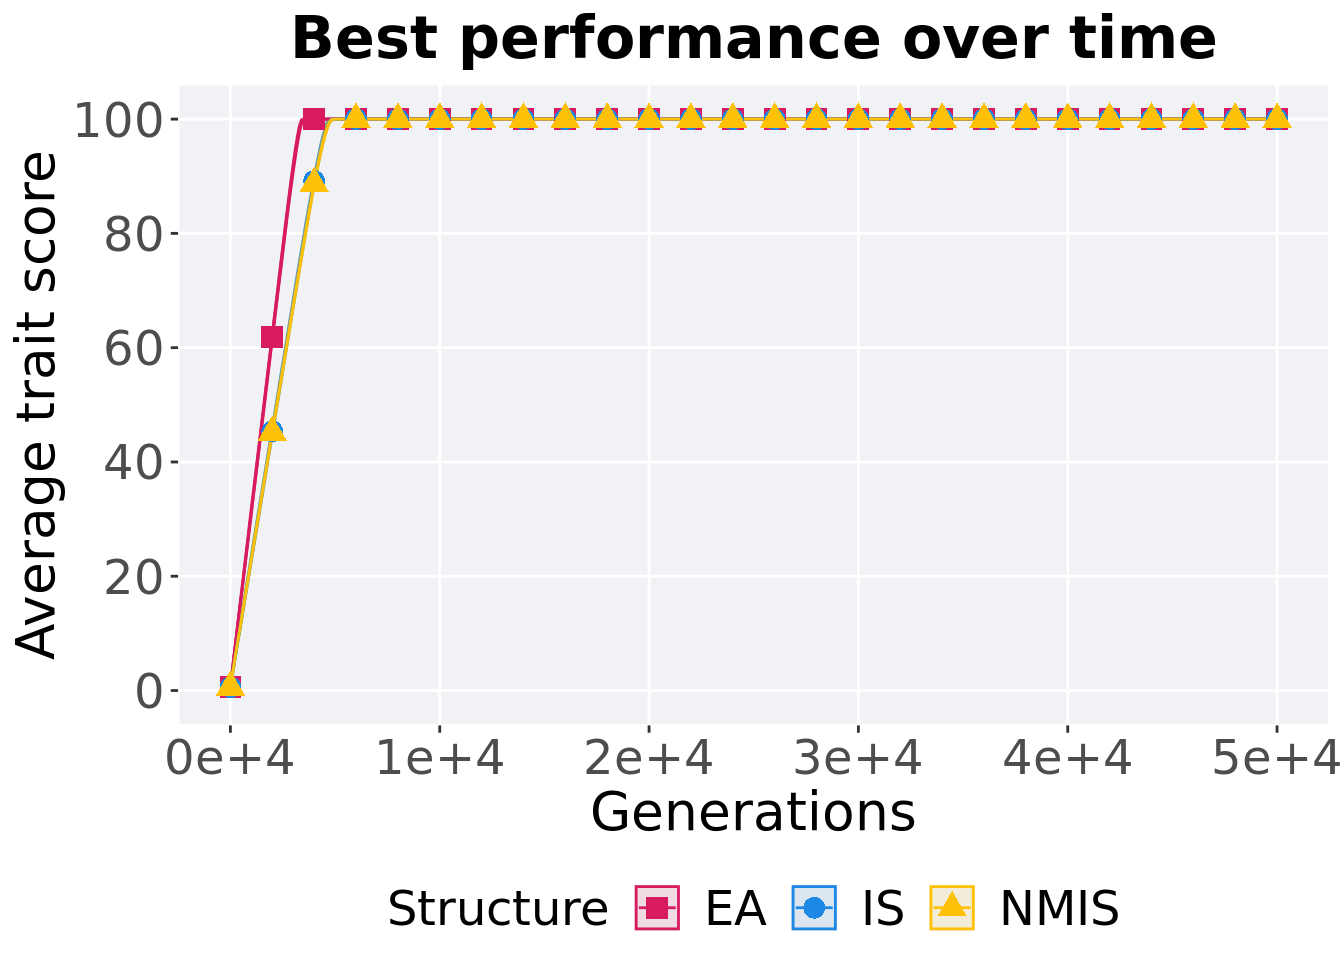
\includegraphics{demo_files/figure-latex/base-tru-exp-perf-1.pdf}

\hypertarget{generation-satisfactory-solution-found}{%
\subsection{Generation satisfactory solution found}\label{generation-satisfactory-solution-found}}

First generation a satisfactory solution is found throughout the 50,000 generations.

\begin{Shaded}
\begin{Highlighting}[]
\KeywordTok{filter}\NormalTok{(base_ssf, Diagnostic }\OperatorTok{==}\StringTok{ 'EXPLOITATION_RATE'} \OperatorTok{&}\StringTok{ `}\DataTypeTok{Selection}\CharTok{\textbackslash{}n}\DataTypeTok{Scheme}\StringTok{`} \OperatorTok{==}\StringTok{ 'TRUNCATION'}\NormalTok{) }\OperatorTok
\StringTok{  }\KeywordTok{ggplot}\NormalTok{(., }\KeywordTok{aes}\NormalTok{(}\DataTypeTok{x =}\NormalTok{ Structure, }\DataTypeTok{y =}\NormalTok{ Generations , }\DataTypeTok{color =}\NormalTok{ Structure, }\DataTypeTok{fill =}\NormalTok{ Structure, }\DataTypeTok{shape =}\NormalTok{ Structure)) }\OperatorTok{+}
\StringTok{  }\KeywordTok{geom_flat_violin}\NormalTok{(}\DataTypeTok{position =} \KeywordTok{position_nudge}\NormalTok{(}\DataTypeTok{x =} \FloatTok{.2}\NormalTok{, }\DataTypeTok{y =} \DecValTok{0}\NormalTok{), }\DataTypeTok{scale =} \StringTok{'width'}\NormalTok{, }\DataTypeTok{alpha =} \FloatTok{0.2}\NormalTok{) }\OperatorTok{+}
\StringTok{  }\KeywordTok{geom_point}\NormalTok{(}\DataTypeTok{position =} \KeywordTok{position_jitter}\NormalTok{(}\DataTypeTok{width =} \FloatTok{.1}\NormalTok{), }\DataTypeTok{size =} \FloatTok{1.5}\NormalTok{, }\DataTypeTok{alpha =} \FloatTok{1.0}\NormalTok{) }\OperatorTok{+}
\StringTok{  }\KeywordTok{geom_boxplot}\NormalTok{(}\DataTypeTok{color =} \StringTok{'black'}\NormalTok{, }\DataTypeTok{width =} \FloatTok{.2}\NormalTok{, }\DataTypeTok{outlier.shape =} \OtherTok{NA}\NormalTok{, }\DataTypeTok{alpha =} \FloatTok{0.0}\NormalTok{) }\OperatorTok{+}
\StringTok{  }\KeywordTok{scale_y_continuous}\NormalTok{(}
    \DataTypeTok{name=}\StringTok{"Generation"}
\NormalTok{  ) }\OperatorTok{+}
\StringTok{  }\KeywordTok{scale_x_discrete}\NormalTok{(}
    \DataTypeTok{name=}\StringTok{"Structure"}
\NormalTok{  )}\OperatorTok{+}
\StringTok{  }\KeywordTok{scale_shape_manual}\NormalTok{(}\DataTypeTok{values=}\NormalTok{SHAPE)}\OperatorTok{+}
\StringTok{  }\KeywordTok{scale_colour_manual}\NormalTok{(}\DataTypeTok{values =}\NormalTok{ cb_palette, ) }\OperatorTok{+}
\StringTok{  }\KeywordTok{scale_fill_manual}\NormalTok{(}\DataTypeTok{values =}\NormalTok{ cb_palette) }\OperatorTok{+}
\StringTok{  }\KeywordTok{ggtitle}\NormalTok{(}\StringTok{'Generation satisfactory solution found'}\NormalTok{)}\OperatorTok{+}
\StringTok{  }\NormalTok{p_theme }\OperatorTok{+}\StringTok{ }\KeywordTok{coord_flip}\NormalTok{()}
\end{Highlighting}
\end{Shaded}

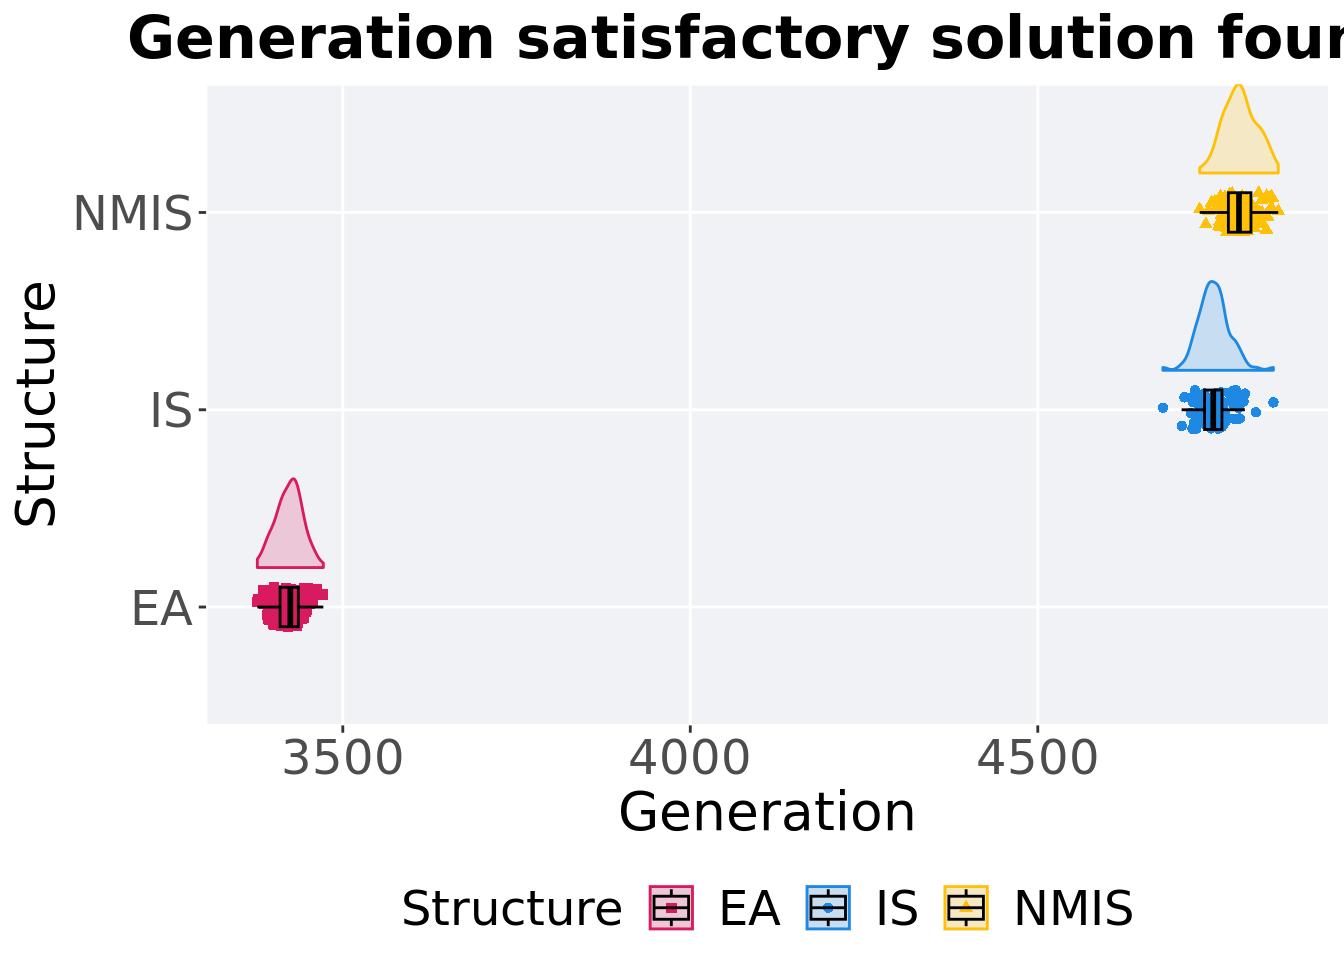
\includegraphics{demo_files/figure-latex/base-tru-exp-ssf-1.pdf}

\hypertarget{stats}{%
\subsection{Stats}\label{stats}}

Summary statistics for the first generation a satisfactory solution is found.

\begin{Shaded}
\begin{Highlighting}[]
\NormalTok{ssf =}\StringTok{ }\KeywordTok{filter}\NormalTok{(base_ssf, Diagnostic }\OperatorTok{==}\StringTok{ 'EXPLOITATION_RATE'} \OperatorTok{&}\StringTok{ `}\DataTypeTok{Selection}\CharTok{\textbackslash{}n}\DataTypeTok{Scheme}\StringTok{`} \OperatorTok{==}\StringTok{ 'TRUNCATION'} \OperatorTok{&}\StringTok{ }\NormalTok{Generations }\OperatorTok{<}\StringTok{ }\DecValTok{60000}\NormalTok{)}
\NormalTok{ssf }\OperatorTok
\StringTok{  }\KeywordTok{group_by}\NormalTok{(Structure) }\OperatorTok
\StringTok{  }\NormalTok{dplyr}\OperatorTok{::}\KeywordTok{summarise}\NormalTok{(}
    \DataTypeTok{count =} \KeywordTok{n}\NormalTok{(),}
    \DataTypeTok{na_cnt =} \KeywordTok{sum}\NormalTok{(}\KeywordTok{is.na}\NormalTok{(Generations)),}
    \DataTypeTok{min =} \KeywordTok{min}\NormalTok{(Generations, }\DataTypeTok{na.rm =} \OtherTok{TRUE}\NormalTok{),}
    \DataTypeTok{median =} \KeywordTok{median}\NormalTok{(Generations, }\DataTypeTok{na.rm =} \OtherTok{TRUE}\NormalTok{),}
    \DataTypeTok{mean =} \KeywordTok{mean}\NormalTok{(Generations, }\DataTypeTok{na.rm =} \OtherTok{TRUE}\NormalTok{),}
    \DataTypeTok{max =} \KeywordTok{max}\NormalTok{(Generations, }\DataTypeTok{na.rm =} \OtherTok{TRUE}\NormalTok{),}
    \DataTypeTok{IQR =} \KeywordTok{IQR}\NormalTok{(Generations, }\DataTypeTok{na.rm =} \OtherTok{TRUE}\NormalTok{)}
\NormalTok{  )}
\end{Highlighting}
\end{Shaded}

\begin{verbatim}
## # A tibble: 3 x 8
##   Structure count na_cnt   min median  mean   max   IQR
##   <fct>     <int>  <int> <int>  <dbl> <dbl> <int> <dbl>
## 1 EA          100      0  3377  3424. 3423.  3472  26.2
## 2 IS          100      0  4680  4752. 4754.  4839  25  
## 3 NMIS        100      0  4733  4790. 4791.  4846  32.5
\end{verbatim}

Kruskal--Wallis test provides evidence of difference among selection schemes.

\begin{Shaded}
\begin{Highlighting}[]
\KeywordTok{kruskal.test}\NormalTok{(Generations }\OperatorTok{~}\StringTok{ }\NormalTok{Structure, }\DataTypeTok{data =}\NormalTok{ ssf)}
\end{Highlighting}
\end{Shaded}

\begin{verbatim}
## 
##  Kruskal-Wallis rank sum test
## 
## data:  Generations by Structure
## Kruskal-Wallis chi-squared = 237.99, df = 2, p-value < 2.2e-16
\end{verbatim}

Results for post-hoc Wilcoxon rank-sum test with a Bonferroni correction.

\begin{Shaded}
\begin{Highlighting}[]
\KeywordTok{pairwise.wilcox.test}\NormalTok{(}\DataTypeTok{x =}\NormalTok{ ssf}\OperatorTok{$}\NormalTok{Generations, }\DataTypeTok{g =}\NormalTok{ ssf}\OperatorTok{$}\NormalTok{Structure, }\DataTypeTok{p.adjust.method =} \StringTok{"bonferroni"}\NormalTok{,}
                     \DataTypeTok{paired =} \OtherTok{FALSE}\NormalTok{, }\DataTypeTok{conf.int =} \OtherTok{FALSE}\NormalTok{, }\DataTypeTok{alternative =} \StringTok{'g'}\NormalTok{)}
\end{Highlighting}
\end{Shaded}

\begin{verbatim}
## 
##  Pairwise comparisons using Wilcoxon rank sum test with continuity correction 
## 
## data:  ssf$Generations and ssf$Structure 
## 
##      EA     IS    
## IS   <2e-16 -     
## NMIS <2e-16 <2e-16
## 
## P value adjustment method: bonferroni
\end{verbatim}

\hypertarget{tournament-selection}{%
\section{Tournament selection}\label{tournament-selection}}

Here we analyze how the different population structures affect tournament selection (size 8) on the exploitation rate diagnostic.

\hypertarget{performance-over-time-1}{%
\subsection{Performance over time}\label{performance-over-time-1}}

\begin{Shaded}
\begin{Highlighting}[]
\NormalTok{lines =}\StringTok{ }\KeywordTok{filter}\NormalTok{(base_over_time, Diagnostic }\OperatorTok{==}\StringTok{ 'EXPLOITATION_RATE'} \OperatorTok{&}\StringTok{ `}\DataTypeTok{Selection}\CharTok{\textbackslash{}n}\DataTypeTok{Scheme}\StringTok{`} \OperatorTok{==}\StringTok{ 'TOURNAMENT'}\NormalTok{) }\OperatorTok
\StringTok{  }\KeywordTok{group_by}\NormalTok{(Structure, Generations) }\OperatorTok
\StringTok{  }\NormalTok{dplyr}\OperatorTok{::}\KeywordTok{summarise}\NormalTok{(}
    \DataTypeTok{min =} \KeywordTok{min}\NormalTok{(pop_fit_max) }\OperatorTok{/}\StringTok{ }\NormalTok{DIMENSIONALITY,}
    \DataTypeTok{mean =} \KeywordTok{mean}\NormalTok{(pop_fit_max) }\OperatorTok{/}\StringTok{ }\NormalTok{DIMENSIONALITY,}
    \DataTypeTok{max =} \KeywordTok{max}\NormalTok{(pop_fit_max) }\OperatorTok{/}\StringTok{ }\NormalTok{DIMENSIONALITY}
\NormalTok{  )}
\KeywordTok{ggplot}\NormalTok{(lines, }\KeywordTok{aes}\NormalTok{(}\DataTypeTok{x=}\NormalTok{Generations, }\DataTypeTok{y=}\NormalTok{mean, }\DataTypeTok{group =}\NormalTok{ Structure, }\DataTypeTok{fill =}\NormalTok{ Structure, }\DataTypeTok{color =}\NormalTok{ Structure, }\DataTypeTok{shape =}\NormalTok{ Structure)) }\OperatorTok{+}
\StringTok{  }\KeywordTok{geom_ribbon}\NormalTok{(}\KeywordTok{aes}\NormalTok{(}\DataTypeTok{ymin =}\NormalTok{ min, }\DataTypeTok{ymax =}\NormalTok{ max), }\DataTypeTok{alpha =} \FloatTok{0.1}\NormalTok{) }\OperatorTok{+}
\StringTok{  }\KeywordTok{geom_line}\NormalTok{(}\DataTypeTok{size =} \FloatTok{0.5}\NormalTok{) }\OperatorTok{+}
\StringTok{  }\KeywordTok{geom_point}\NormalTok{(}\DataTypeTok{data =} \KeywordTok{filter}\NormalTok{(lines, Generations }\OperatorTok\StringTok{ }\DecValTok{2000} \OperatorTok{==}\StringTok{ }\DecValTok{0}\NormalTok{), }\DataTypeTok{size =} \FloatTok{2.5}\NormalTok{, }\DataTypeTok{stroke =} \FloatTok{2.0}\NormalTok{, }\DataTypeTok{alpha =} \FloatTok{1.0}\NormalTok{) }\OperatorTok{+}
\StringTok{  }\KeywordTok{scale_y_continuous}\NormalTok{(}
    \DataTypeTok{name=}\StringTok{"Average trait score"}\NormalTok{,}
    \DataTypeTok{limits=}\KeywordTok{c}\NormalTok{(}\OperatorTok{-}\DecValTok{1}\NormalTok{, }\DecValTok{101}\NormalTok{),}
    \DataTypeTok{breaks=}\KeywordTok{seq}\NormalTok{(}\DecValTok{0}\NormalTok{,}\DecValTok{100}\NormalTok{, }\DecValTok{20}\NormalTok{),}
    \DataTypeTok{labels=}\KeywordTok{c}\NormalTok{(}\StringTok{"0"}\NormalTok{, }\StringTok{"20"}\NormalTok{, }\StringTok{"40"}\NormalTok{, }\StringTok{"60"}\NormalTok{, }\StringTok{"80"}\NormalTok{, }\StringTok{"100"}\NormalTok{)}
\NormalTok{  ) }\OperatorTok{+}
\StringTok{  }\KeywordTok{scale_x_continuous}\NormalTok{(}
    \DataTypeTok{name=}\StringTok{"Generations"}\NormalTok{,}
    \DataTypeTok{limits=}\KeywordTok{c}\NormalTok{(}\DecValTok{0}\NormalTok{, }\DecValTok{50000}\NormalTok{),}
    \DataTypeTok{breaks=}\KeywordTok{c}\NormalTok{(}\DecValTok{0}\NormalTok{, }\DecValTok{10000}\NormalTok{, }\DecValTok{20000}\NormalTok{, }\DecValTok{30000}\NormalTok{, }\DecValTok{40000}\NormalTok{, }\DecValTok{50000}\NormalTok{),}
    \DataTypeTok{labels=}\KeywordTok{c}\NormalTok{(}\StringTok{"0e+4"}\NormalTok{, }\StringTok{"1e+4"}\NormalTok{, }\StringTok{"2e+4"}\NormalTok{, }\StringTok{"3e+4"}\NormalTok{, }\StringTok{"4e+4"}\NormalTok{, }\StringTok{"5e+4"}\NormalTok{)}

\NormalTok{  ) }\OperatorTok{+}
\StringTok{  }\KeywordTok{scale_shape_manual}\NormalTok{(}\DataTypeTok{values=}\NormalTok{SHAPE)}\OperatorTok{+}
\StringTok{  }\KeywordTok{scale_colour_manual}\NormalTok{(}\DataTypeTok{values =}\NormalTok{ cb_palette) }\OperatorTok{+}
\StringTok{  }\KeywordTok{scale_fill_manual}\NormalTok{(}\DataTypeTok{values =}\NormalTok{ cb_palette) }\OperatorTok{+}
\StringTok{  }\KeywordTok{ggtitle}\NormalTok{(}\StringTok{"Best performance over time"}\NormalTok{) }\OperatorTok{+}
\StringTok{  }\NormalTok{p_theme}
\end{Highlighting}
\end{Shaded}

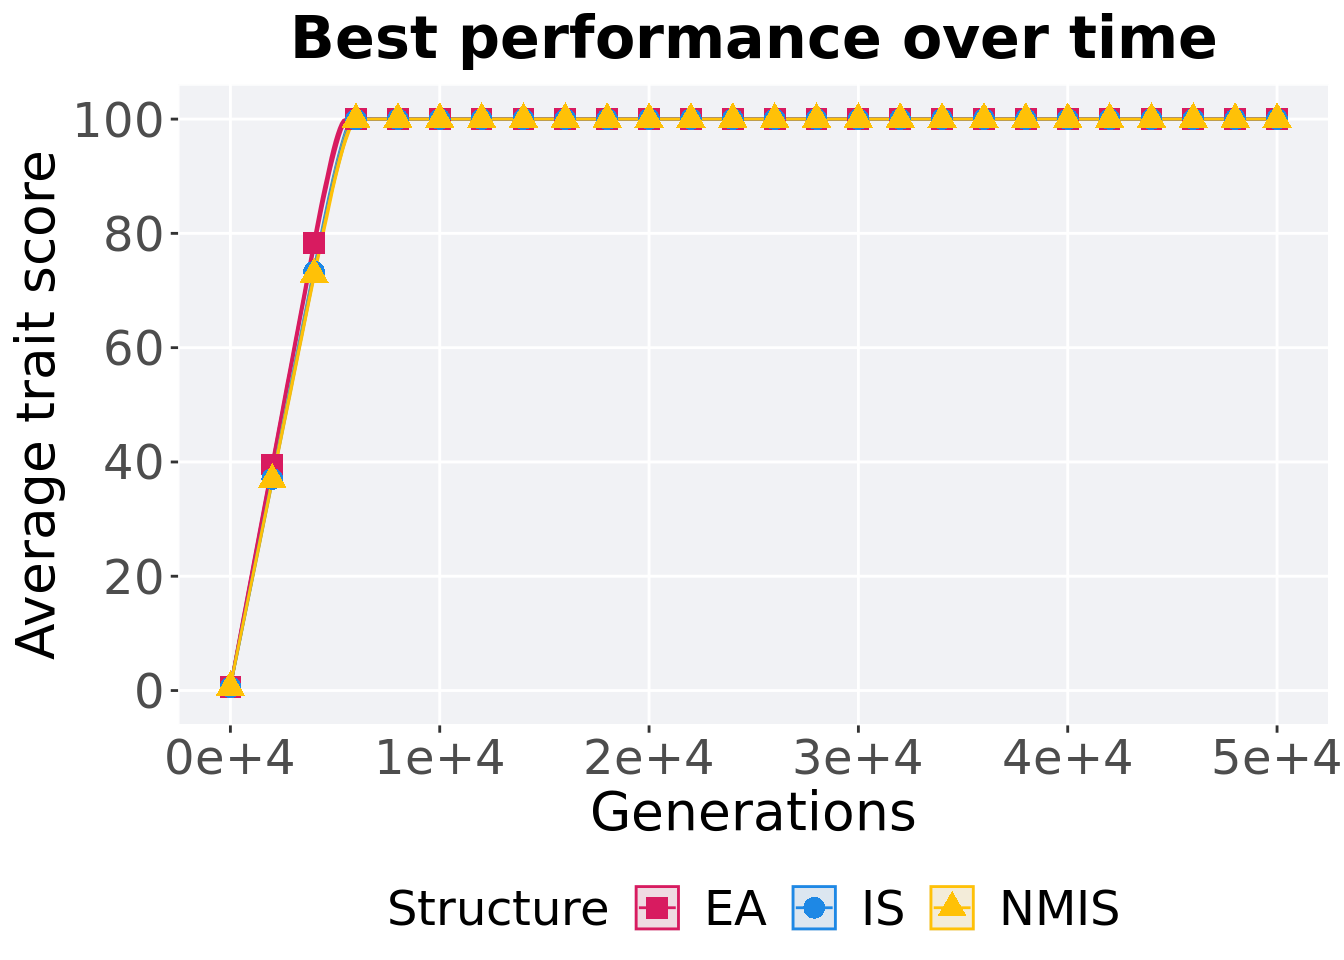
\includegraphics{demo_files/figure-latex/base-tor-exp-perf-1.pdf}

\hypertarget{generation-satisfactory-solution-found-1}{%
\subsection{Generation satisfactory solution found}\label{generation-satisfactory-solution-found-1}}

First generation a satisfactory solution is found throughout the 50,000 generations.

\begin{Shaded}
\begin{Highlighting}[]
\KeywordTok{filter}\NormalTok{(base_ssf, Diagnostic }\OperatorTok{==}\StringTok{ 'EXPLOITATION_RATE'} \OperatorTok{&}\StringTok{ `}\DataTypeTok{Selection}\CharTok{\textbackslash{}n}\DataTypeTok{Scheme}\StringTok{`} \OperatorTok{==}\StringTok{ 'TOURNAMENT'}\NormalTok{) }\OperatorTok
\StringTok{  }\KeywordTok{ggplot}\NormalTok{(., }\KeywordTok{aes}\NormalTok{(}\DataTypeTok{x =}\NormalTok{ Structure, }\DataTypeTok{y =}\NormalTok{ Generations , }\DataTypeTok{color =}\NormalTok{ Structure, }\DataTypeTok{fill =}\NormalTok{ Structure, }\DataTypeTok{shape =}\NormalTok{ Structure)) }\OperatorTok{+}
\StringTok{  }\KeywordTok{geom_flat_violin}\NormalTok{(}\DataTypeTok{position =} \KeywordTok{position_nudge}\NormalTok{(}\DataTypeTok{x =} \FloatTok{.2}\NormalTok{, }\DataTypeTok{y =} \DecValTok{0}\NormalTok{), }\DataTypeTok{scale =} \StringTok{'width'}\NormalTok{, }\DataTypeTok{alpha =} \FloatTok{0.2}\NormalTok{) }\OperatorTok{+}
\StringTok{  }\KeywordTok{geom_point}\NormalTok{(}\DataTypeTok{position =} \KeywordTok{position_jitter}\NormalTok{(}\DataTypeTok{width =} \FloatTok{.1}\NormalTok{), }\DataTypeTok{size =} \FloatTok{1.5}\NormalTok{, }\DataTypeTok{alpha =} \FloatTok{1.0}\NormalTok{) }\OperatorTok{+}
\StringTok{  }\KeywordTok{geom_boxplot}\NormalTok{(}\DataTypeTok{color =} \StringTok{'black'}\NormalTok{, }\DataTypeTok{width =} \FloatTok{.2}\NormalTok{, }\DataTypeTok{outlier.shape =} \OtherTok{NA}\NormalTok{, }\DataTypeTok{alpha =} \FloatTok{0.0}\NormalTok{) }\OperatorTok{+}
\StringTok{  }\KeywordTok{scale_y_continuous}\NormalTok{(}
    \DataTypeTok{name=}\StringTok{"Generation"}
\NormalTok{  ) }\OperatorTok{+}
\StringTok{  }\KeywordTok{scale_x_discrete}\NormalTok{(}
    \DataTypeTok{name=}\StringTok{"Structure"}
\NormalTok{  )}\OperatorTok{+}
\StringTok{  }\KeywordTok{scale_shape_manual}\NormalTok{(}\DataTypeTok{values=}\NormalTok{SHAPE)}\OperatorTok{+}
\StringTok{  }\KeywordTok{scale_colour_manual}\NormalTok{(}\DataTypeTok{values =}\NormalTok{ cb_palette, ) }\OperatorTok{+}
\StringTok{  }\KeywordTok{scale_fill_manual}\NormalTok{(}\DataTypeTok{values =}\NormalTok{ cb_palette) }\OperatorTok{+}
\StringTok{  }\KeywordTok{ggtitle}\NormalTok{(}\StringTok{'Generation satisfactory solution found'}\NormalTok{)}\OperatorTok{+}
\StringTok{  }\NormalTok{p_theme }\OperatorTok{+}\StringTok{ }\KeywordTok{coord_flip}\NormalTok{()}
\end{Highlighting}
\end{Shaded}

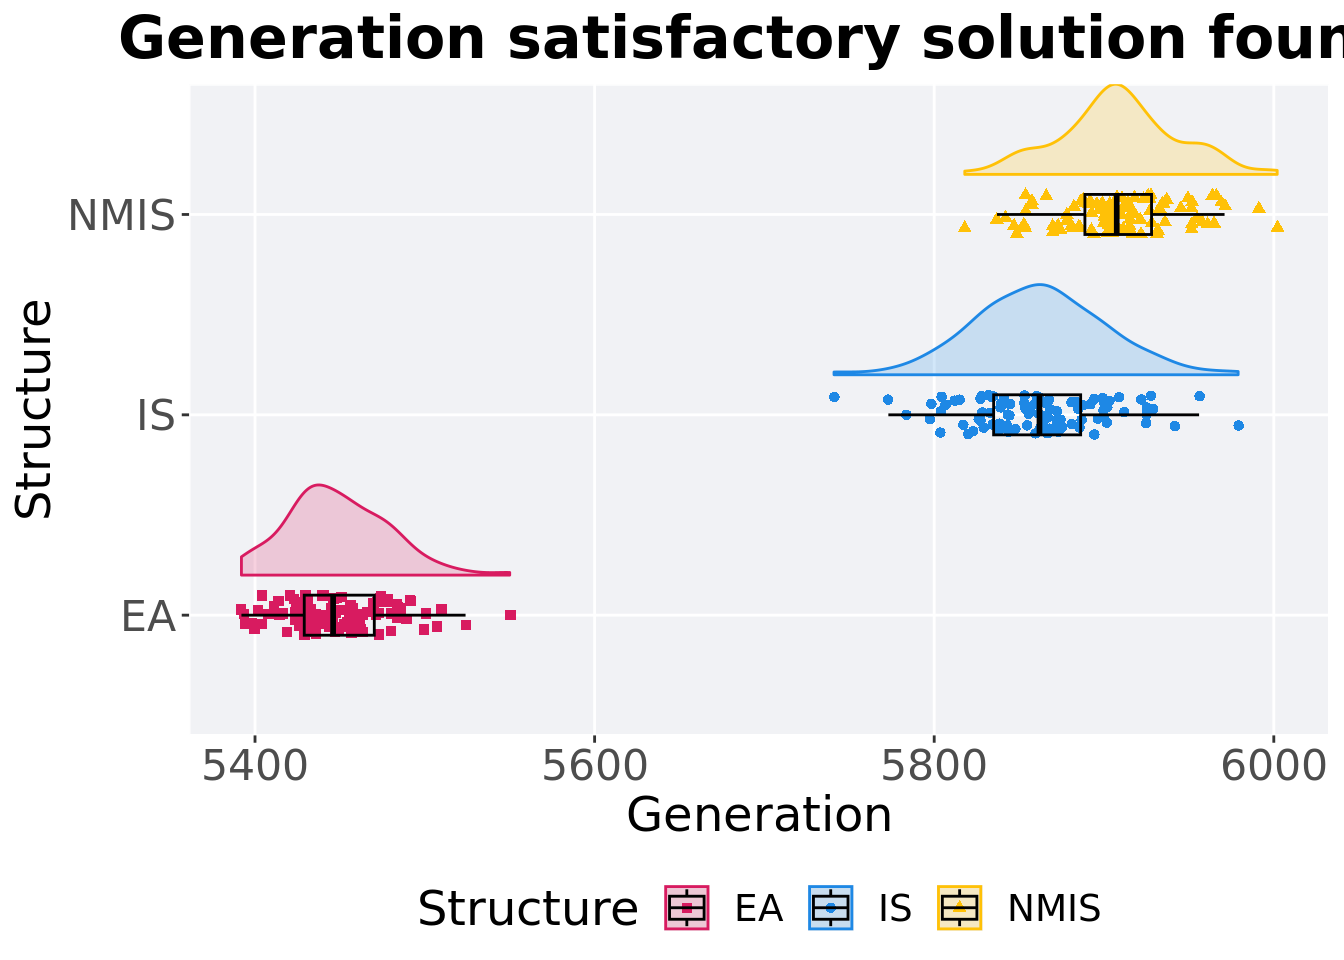
\includegraphics{demo_files/figure-latex/base-tor-exp-ssf-1.pdf}

\hypertarget{stats-1}{%
\subsection{Stats}\label{stats-1}}

Summary statistics for the first generation a satisfactory solution is found.

\begin{Shaded}
\begin{Highlighting}[]
\NormalTok{ssf =}\StringTok{ }\KeywordTok{filter}\NormalTok{(base_ssf, Diagnostic }\OperatorTok{==}\StringTok{ 'EXPLOITATION_RATE'} \OperatorTok{&}\StringTok{ `}\DataTypeTok{Selection}\CharTok{\textbackslash{}n}\DataTypeTok{Scheme}\StringTok{`} \OperatorTok{==}\StringTok{ 'TOURNAMENT'} \OperatorTok{&}\StringTok{ }\NormalTok{Generations }\OperatorTok{<}\StringTok{ }\DecValTok{60000}\NormalTok{)}
\NormalTok{ssf }\OperatorTok
\StringTok{  }\KeywordTok{group_by}\NormalTok{(Structure) }\OperatorTok
\StringTok{  }\NormalTok{dplyr}\OperatorTok{::}\KeywordTok{summarise}\NormalTok{(}
    \DataTypeTok{count =} \KeywordTok{n}\NormalTok{(),}
    \DataTypeTok{na_cnt =} \KeywordTok{sum}\NormalTok{(}\KeywordTok{is.na}\NormalTok{(Generations)),}
    \DataTypeTok{min =} \KeywordTok{min}\NormalTok{(Generations, }\DataTypeTok{na.rm =} \OtherTok{TRUE}\NormalTok{),}
    \DataTypeTok{median =} \KeywordTok{median}\NormalTok{(Generations, }\DataTypeTok{na.rm =} \OtherTok{TRUE}\NormalTok{),}
    \DataTypeTok{mean =} \KeywordTok{mean}\NormalTok{(Generations, }\DataTypeTok{na.rm =} \OtherTok{TRUE}\NormalTok{),}
    \DataTypeTok{max =} \KeywordTok{max}\NormalTok{(Generations, }\DataTypeTok{na.rm =} \OtherTok{TRUE}\NormalTok{),}
    \DataTypeTok{IQR =} \KeywordTok{IQR}\NormalTok{(Generations, }\DataTypeTok{na.rm =} \OtherTok{TRUE}\NormalTok{)}
\NormalTok{  )}
\end{Highlighting}
\end{Shaded}

\begin{verbatim}
## # A tibble: 3 x 8
##   Structure count na_cnt   min median  mean   max   IQR
##   <fct>     <int>  <int> <int>  <dbl> <dbl> <int> <dbl>
## 1 EA          100      0  5392  5446  5449.  5550  41.2
## 2 IS          100      0  5741  5862  5862.  5979  51.2
## 3 NMIS        100      0  5818  5908. 5909.  6002  39.2
\end{verbatim}

Kruskal--Wallis test provides evidence of difference among selection schemes.

\begin{Shaded}
\begin{Highlighting}[]
\KeywordTok{kruskal.test}\NormalTok{(Generations }\OperatorTok{~}\StringTok{ }\NormalTok{Structure, }\DataTypeTok{data =}\NormalTok{ ssf)}
\end{Highlighting}
\end{Shaded}

\begin{verbatim}
## 
##  Kruskal-Wallis rank sum test
## 
## data:  Generations by Structure
## Kruskal-Wallis chi-squared = 226.27, df = 2, p-value < 2.2e-16
\end{verbatim}

Results for post-hoc Wilcoxon rank-sum test with a Bonferroni correction.

\begin{Shaded}
\begin{Highlighting}[]
\KeywordTok{pairwise.wilcox.test}\NormalTok{(}\DataTypeTok{x =}\NormalTok{ ssf}\OperatorTok{$}\NormalTok{Generations, }\DataTypeTok{g =}\NormalTok{ ssf}\OperatorTok{$}\NormalTok{Structure, }\DataTypeTok{p.adjust.method =} \StringTok{"bonferroni"}\NormalTok{,}
                     \DataTypeTok{paired =} \OtherTok{FALSE}\NormalTok{, }\DataTypeTok{conf.int =} \OtherTok{FALSE}\NormalTok{, }\DataTypeTok{alternative =} \StringTok{'g'}\NormalTok{)}
\end{Highlighting}
\end{Shaded}

\begin{verbatim}
## 
##  Pairwise comparisons using Wilcoxon rank sum test with continuity correction 
## 
## data:  ssf$Generations and ssf$Structure 
## 
##      EA      IS     
## IS   < 2e-16 -      
## NMIS < 2e-16 1.1e-14
## 
## P value adjustment method: bonferroni
\end{verbatim}

\hypertarget{lexicase-selection}{%
\section{Lexicase selection}\label{lexicase-selection}}

Here we analyze how the different population structures affect standard lexicase selection on the exploitation rate diagnostic.

\hypertarget{performance-over-time-2}{%
\subsection{Performance over time}\label{performance-over-time-2}}

\begin{Shaded}
\begin{Highlighting}[]
\NormalTok{lines =}\StringTok{ }\KeywordTok{filter}\NormalTok{(base_over_time, Diagnostic }\OperatorTok{==}\StringTok{ 'EXPLOITATION_RATE'} \OperatorTok{&}\StringTok{ `}\DataTypeTok{Selection}\CharTok{\textbackslash{}n}\DataTypeTok{Scheme}\StringTok{`} \OperatorTok{==}\StringTok{ 'LEXICASE'}\NormalTok{) }\OperatorTok
\StringTok{  }\KeywordTok{group_by}\NormalTok{(Structure, Generations) }\OperatorTok
\StringTok{  }\NormalTok{dplyr}\OperatorTok{::}\KeywordTok{summarise}\NormalTok{(}
    \DataTypeTok{min =} \KeywordTok{min}\NormalTok{(pop_fit_max) }\OperatorTok{/}\StringTok{ }\NormalTok{DIMENSIONALITY,}
    \DataTypeTok{mean =} \KeywordTok{mean}\NormalTok{(pop_fit_max) }\OperatorTok{/}\StringTok{ }\NormalTok{DIMENSIONALITY,}
    \DataTypeTok{max =} \KeywordTok{max}\NormalTok{(pop_fit_max) }\OperatorTok{/}\StringTok{ }\NormalTok{DIMENSIONALITY}
\NormalTok{  )}
\KeywordTok{ggplot}\NormalTok{(lines, }\KeywordTok{aes}\NormalTok{(}\DataTypeTok{x=}\NormalTok{Generations, }\DataTypeTok{y=}\NormalTok{mean, }\DataTypeTok{group =}\NormalTok{ Structure, }\DataTypeTok{fill =}\NormalTok{ Structure, }\DataTypeTok{color =}\NormalTok{ Structure, }\DataTypeTok{shape =}\NormalTok{ Structure)) }\OperatorTok{+}
\StringTok{  }\KeywordTok{geom_ribbon}\NormalTok{(}\KeywordTok{aes}\NormalTok{(}\DataTypeTok{ymin =}\NormalTok{ min, }\DataTypeTok{ymax =}\NormalTok{ max), }\DataTypeTok{alpha =} \FloatTok{0.1}\NormalTok{) }\OperatorTok{+}
\StringTok{  }\KeywordTok{geom_line}\NormalTok{(}\DataTypeTok{size =} \FloatTok{0.5}\NormalTok{) }\OperatorTok{+}
\StringTok{  }\KeywordTok{geom_point}\NormalTok{(}\DataTypeTok{data =} \KeywordTok{filter}\NormalTok{(lines, Generations }\OperatorTok\StringTok{ }\DecValTok{2000} \OperatorTok{==}\StringTok{ }\DecValTok{0}\NormalTok{), }\DataTypeTok{size =} \FloatTok{2.5}\NormalTok{, }\DataTypeTok{stroke =} \FloatTok{2.0}\NormalTok{, }\DataTypeTok{alpha =} \FloatTok{1.0}\NormalTok{) }\OperatorTok{+}
\StringTok{  }\KeywordTok{scale_y_continuous}\NormalTok{(}
    \DataTypeTok{name=}\StringTok{"Average trait score"}\NormalTok{,}
    \DataTypeTok{limits=}\KeywordTok{c}\NormalTok{(}\OperatorTok{-}\DecValTok{1}\NormalTok{, }\DecValTok{101}\NormalTok{),}
    \DataTypeTok{breaks=}\KeywordTok{seq}\NormalTok{(}\DecValTok{0}\NormalTok{,}\DecValTok{100}\NormalTok{, }\DecValTok{20}\NormalTok{),}
    \DataTypeTok{labels=}\KeywordTok{c}\NormalTok{(}\StringTok{"0"}\NormalTok{, }\StringTok{"20"}\NormalTok{, }\StringTok{"40"}\NormalTok{, }\StringTok{"60"}\NormalTok{, }\StringTok{"80"}\NormalTok{, }\StringTok{"100"}\NormalTok{)}
\NormalTok{  ) }\OperatorTok{+}
\StringTok{  }\KeywordTok{scale_x_continuous}\NormalTok{(}
    \DataTypeTok{name=}\StringTok{"Generations"}\NormalTok{,}
    \DataTypeTok{limits=}\KeywordTok{c}\NormalTok{(}\DecValTok{0}\NormalTok{, }\DecValTok{50000}\NormalTok{),}
    \DataTypeTok{breaks=}\KeywordTok{c}\NormalTok{(}\DecValTok{0}\NormalTok{, }\DecValTok{10000}\NormalTok{, }\DecValTok{20000}\NormalTok{, }\DecValTok{30000}\NormalTok{, }\DecValTok{40000}\NormalTok{, }\DecValTok{50000}\NormalTok{),}
    \DataTypeTok{labels=}\KeywordTok{c}\NormalTok{(}\StringTok{"0e+4"}\NormalTok{, }\StringTok{"1e+4"}\NormalTok{, }\StringTok{"2e+4"}\NormalTok{, }\StringTok{"3e+4"}\NormalTok{, }\StringTok{"4e+4"}\NormalTok{, }\StringTok{"5e+4"}\NormalTok{)}

\NormalTok{  ) }\OperatorTok{+}
\StringTok{  }\KeywordTok{scale_shape_manual}\NormalTok{(}\DataTypeTok{values=}\NormalTok{SHAPE)}\OperatorTok{+}
\StringTok{  }\KeywordTok{scale_colour_manual}\NormalTok{(}\DataTypeTok{values =}\NormalTok{ cb_palette) }\OperatorTok{+}
\StringTok{  }\KeywordTok{scale_fill_manual}\NormalTok{(}\DataTypeTok{values =}\NormalTok{ cb_palette) }\OperatorTok{+}
\StringTok{  }\KeywordTok{ggtitle}\NormalTok{(}\StringTok{"Best performance over time"}\NormalTok{) }\OperatorTok{+}
\StringTok{  }\NormalTok{p_theme}
\end{Highlighting}
\end{Shaded}

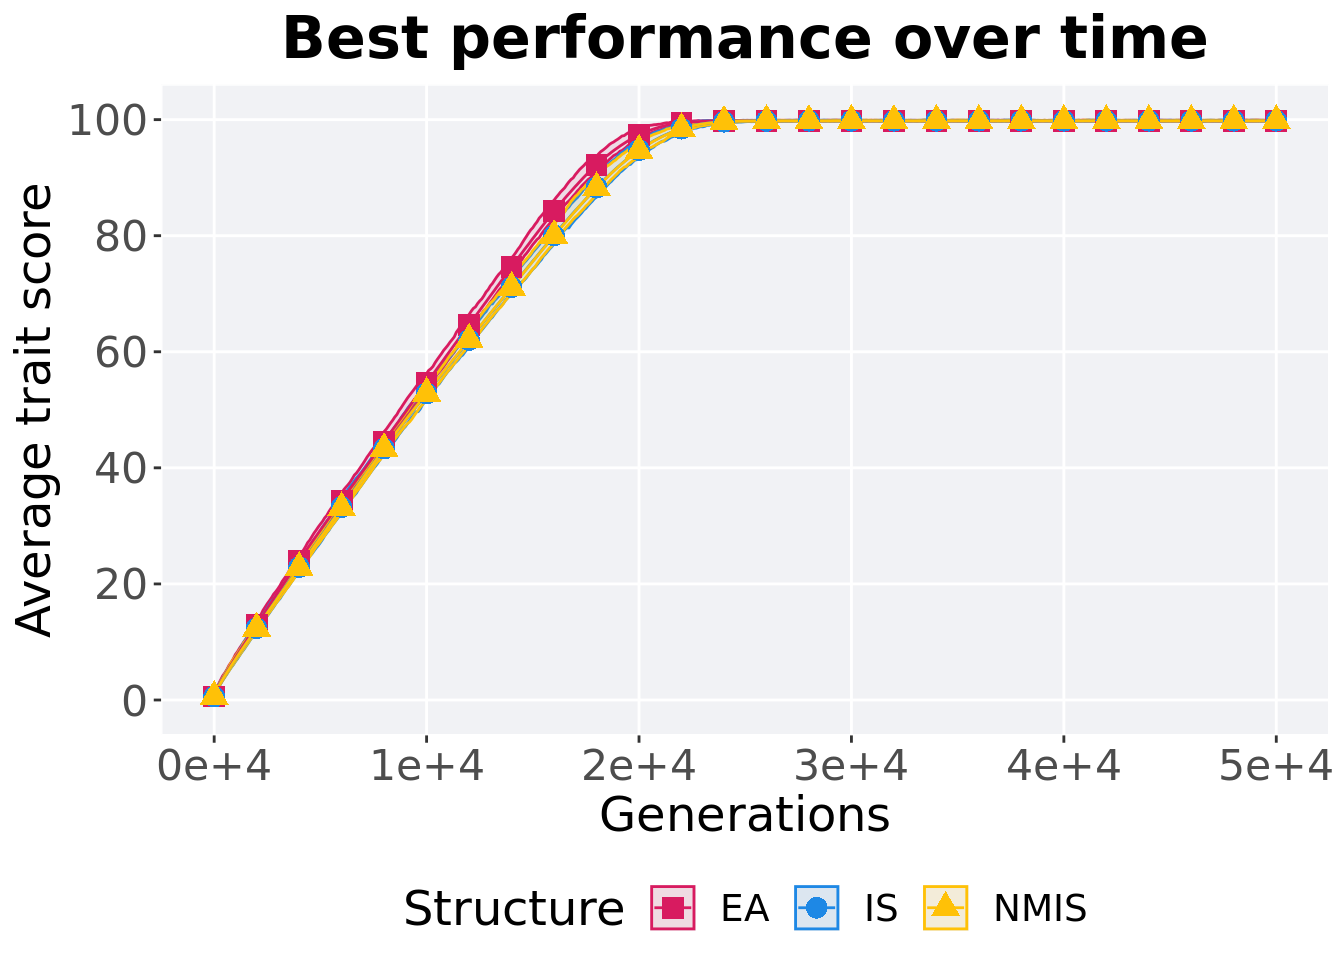
\includegraphics{demo_files/figure-latex/base-lex-exp-perf-1.pdf}

\hypertarget{generation-satisfactory-solution-found-2}{%
\subsection{Generation satisfactory solution found}\label{generation-satisfactory-solution-found-2}}

First generation a satisfactory solution is found throughout the 50,000 generations.

\begin{Shaded}
\begin{Highlighting}[]
\KeywordTok{filter}\NormalTok{(base_ssf, Diagnostic }\OperatorTok{==}\StringTok{ 'EXPLOITATION_RATE'} \OperatorTok{&}\StringTok{ `}\DataTypeTok{Selection}\CharTok{\textbackslash{}n}\DataTypeTok{Scheme}\StringTok{`} \OperatorTok{==}\StringTok{ 'LEXICASE'}\NormalTok{) }\OperatorTok
\StringTok{  }\KeywordTok{ggplot}\NormalTok{(., }\KeywordTok{aes}\NormalTok{(}\DataTypeTok{x =}\NormalTok{ Structure, }\DataTypeTok{y =}\NormalTok{ Generations , }\DataTypeTok{color =}\NormalTok{ Structure, }\DataTypeTok{fill =}\NormalTok{ Structure, }\DataTypeTok{shape =}\NormalTok{ Structure)) }\OperatorTok{+}
\StringTok{  }\KeywordTok{geom_flat_violin}\NormalTok{(}\DataTypeTok{position =} \KeywordTok{position_nudge}\NormalTok{(}\DataTypeTok{x =} \FloatTok{.2}\NormalTok{, }\DataTypeTok{y =} \DecValTok{0}\NormalTok{), }\DataTypeTok{scale =} \StringTok{'width'}\NormalTok{, }\DataTypeTok{alpha =} \FloatTok{0.2}\NormalTok{) }\OperatorTok{+}
\StringTok{  }\KeywordTok{geom_point}\NormalTok{(}\DataTypeTok{position =} \KeywordTok{position_jitter}\NormalTok{(}\DataTypeTok{width =} \FloatTok{.1}\NormalTok{), }\DataTypeTok{size =} \FloatTok{1.5}\NormalTok{, }\DataTypeTok{alpha =} \FloatTok{1.0}\NormalTok{) }\OperatorTok{+}
\StringTok{  }\KeywordTok{geom_boxplot}\NormalTok{(}\DataTypeTok{color =} \StringTok{'black'}\NormalTok{, }\DataTypeTok{width =} \FloatTok{.2}\NormalTok{, }\DataTypeTok{outlier.shape =} \OtherTok{NA}\NormalTok{, }\DataTypeTok{alpha =} \FloatTok{0.0}\NormalTok{) }\OperatorTok{+}
\StringTok{  }\KeywordTok{scale_y_continuous}\NormalTok{(}
    \DataTypeTok{name=}\StringTok{"Generation"}
\NormalTok{  ) }\OperatorTok{+}
\StringTok{  }\KeywordTok{scale_x_discrete}\NormalTok{(}
    \DataTypeTok{name=}\StringTok{"Structure"}
\NormalTok{  )}\OperatorTok{+}
\StringTok{  }\KeywordTok{scale_shape_manual}\NormalTok{(}\DataTypeTok{values=}\NormalTok{SHAPE)}\OperatorTok{+}
\StringTok{  }\KeywordTok{scale_colour_manual}\NormalTok{(}\DataTypeTok{values =}\NormalTok{ cb_palette, ) }\OperatorTok{+}
\StringTok{  }\KeywordTok{scale_fill_manual}\NormalTok{(}\DataTypeTok{values =}\NormalTok{ cb_palette) }\OperatorTok{+}
\StringTok{  }\KeywordTok{ggtitle}\NormalTok{(}\StringTok{'Generation satisfactory solution found'}\NormalTok{)}\OperatorTok{+}
\StringTok{  }\NormalTok{p_theme }\OperatorTok{+}\StringTok{ }\KeywordTok{coord_flip}\NormalTok{()}
\end{Highlighting}
\end{Shaded}

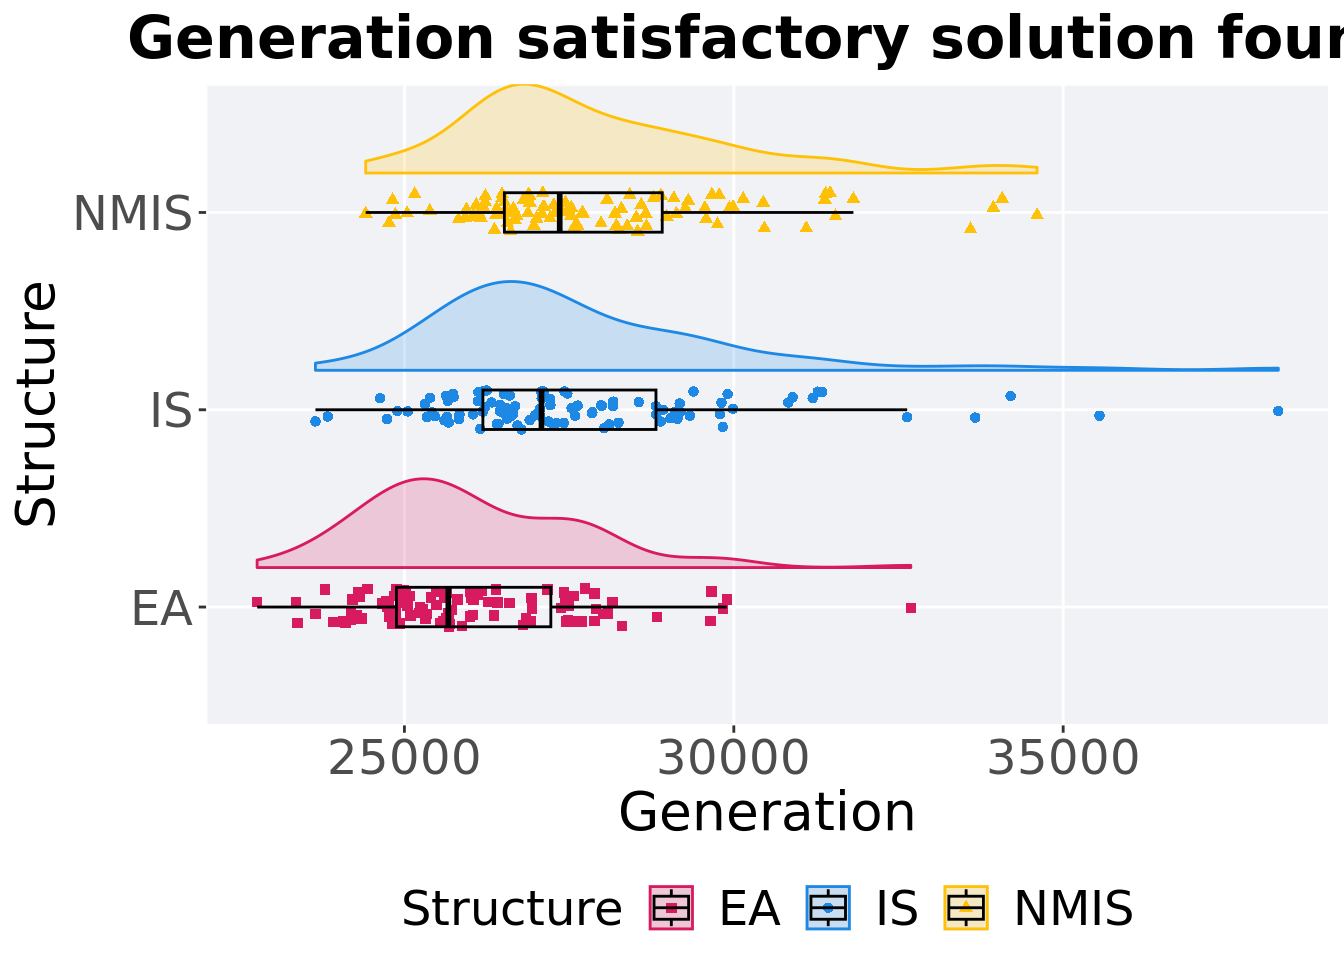
\includegraphics{demo_files/figure-latex/base-lex-exp-ssf-1.pdf}

\hypertarget{stats-2}{%
\subsection{Stats}\label{stats-2}}

Summary statistics for the first generation a satisfactory solution is found.

\begin{Shaded}
\begin{Highlighting}[]
\NormalTok{ssf =}\StringTok{ }\KeywordTok{filter}\NormalTok{(base_ssf, Diagnostic }\OperatorTok{==}\StringTok{ 'EXPLOITATION_RATE'} \OperatorTok{&}\StringTok{ `}\DataTypeTok{Selection}\CharTok{\textbackslash{}n}\DataTypeTok{Scheme}\StringTok{`} \OperatorTok{==}\StringTok{ 'LEXICASE'} \OperatorTok{&}\StringTok{ }\NormalTok{Generations }\OperatorTok{<}\StringTok{ }\DecValTok{60000}\NormalTok{)}
\NormalTok{ssf }\OperatorTok
\StringTok{  }\KeywordTok{group_by}\NormalTok{(Structure) }\OperatorTok
\StringTok{  }\NormalTok{dplyr}\OperatorTok{::}\KeywordTok{summarise}\NormalTok{(}
    \DataTypeTok{count =} \KeywordTok{n}\NormalTok{(),}
    \DataTypeTok{na_cnt =} \KeywordTok{sum}\NormalTok{(}\KeywordTok{is.na}\NormalTok{(Generations)),}
    \DataTypeTok{min =} \KeywordTok{min}\NormalTok{(Generations, }\DataTypeTok{na.rm =} \OtherTok{TRUE}\NormalTok{),}
    \DataTypeTok{median =} \KeywordTok{median}\NormalTok{(Generations, }\DataTypeTok{na.rm =} \OtherTok{TRUE}\NormalTok{),}
    \DataTypeTok{mean =} \KeywordTok{mean}\NormalTok{(Generations, }\DataTypeTok{na.rm =} \OtherTok{TRUE}\NormalTok{),}
    \DataTypeTok{max =} \KeywordTok{max}\NormalTok{(Generations, }\DataTypeTok{na.rm =} \OtherTok{TRUE}\NormalTok{),}
    \DataTypeTok{IQR =} \KeywordTok{IQR}\NormalTok{(Generations, }\DataTypeTok{na.rm =} \OtherTok{TRUE}\NormalTok{)}
\NormalTok{  )}
\end{Highlighting}
\end{Shaded}

\begin{verbatim}
## # A tibble: 3 x 8
##   Structure count na_cnt   min median   mean   max   IQR
##   <fct>     <int>  <int> <int>  <dbl>  <dbl> <int> <dbl>
## 1 EA          100      0 22764 25666. 26026. 32687 2344 
## 2 IS          100      0 23649 27080. 27635. 38266 2628.
## 3 NMIS        100      0 24412 27358. 27906. 34604 2396.
\end{verbatim}

Kruskal--Wallis test provides evidence of difference among selection schemes.

\begin{Shaded}
\begin{Highlighting}[]
\KeywordTok{kruskal.test}\NormalTok{(Generations }\OperatorTok{~}\StringTok{ }\NormalTok{Structure, }\DataTypeTok{data =}\NormalTok{ ssf)}
\end{Highlighting}
\end{Shaded}

\begin{verbatim}
## 
##  Kruskal-Wallis rank sum test
## 
## data:  Generations by Structure
## Kruskal-Wallis chi-squared = 52.814, df = 2, p-value = 3.401e-12
\end{verbatim}

Results for post-hoc Wilcoxon rank-sum test with a Bonferroni correction.

\begin{Shaded}
\begin{Highlighting}[]
\KeywordTok{pairwise.wilcox.test}\NormalTok{(}\DataTypeTok{x =}\NormalTok{ ssf}\OperatorTok{$}\NormalTok{Generations, }\DataTypeTok{g =}\NormalTok{ ssf}\OperatorTok{$}\NormalTok{Structure, }\DataTypeTok{p.adjust.method =} \StringTok{"bonferroni"}\NormalTok{,}
                     \DataTypeTok{paired =} \OtherTok{FALSE}\NormalTok{, }\DataTypeTok{conf.int =} \OtherTok{FALSE}\NormalTok{, }\DataTypeTok{alternative =} \StringTok{'g'}\NormalTok{)}
\end{Highlighting}
\end{Shaded}

\begin{verbatim}
## 
##  Pairwise comparisons using Wilcoxon rank sum test with continuity correction 
## 
## data:  ssf$Generations and ssf$Structure 
## 
##      EA      IS  
## IS   3.0e-08 -   
## NMIS 2.2e-11 0.24
## 
## P value adjustment method: bonferroni
\end{verbatim}

\hypertarget{ordered-exploitation-results}{%
\chapter{Ordered exploitation results}\label{ordered-exploitation-results}}

Here we present the results for \textbf{best performances} found by each selection scheme replicate on the ordered exploitation diagnostic with our base configurations.
Best performance found refers to the largest average trait score found in a given population.
Note that performance values fall between 0.0 and 100.0.
For our base configuration, we execute migrations every 500 generations and there are 4 islands in a ring topology.
When migrations occur, we swap two individuals (same position on each island) and guarantee that no solution can return to the same island.

\hypertarget{analysis-dependencies-1}{%
\section{Analysis dependencies}\label{analysis-dependencies-1}}

\begin{Shaded}
\begin{Highlighting}[]
\KeywordTok{library}\NormalTok{(ggplot2)}
\KeywordTok{library}\NormalTok{(cowplot)}
\KeywordTok{library}\NormalTok{(dplyr)}
\KeywordTok{library}\NormalTok{(PupillometryR)}
\end{Highlighting}
\end{Shaded}

\hypertarget{truncation-selection-1}{%
\section{Truncation selection}\label{truncation-selection-1}}

Here we analyze how the different population structures affect truncation selection (size 8) on the ordered exploitation diagnostic.

\hypertarget{performance-over-time-3}{%
\subsection{Performance over time}\label{performance-over-time-3}}

\begin{Shaded}
\begin{Highlighting}[]
\NormalTok{lines =}\StringTok{ }\KeywordTok{filter}\NormalTok{(base_over_time, Diagnostic }\OperatorTok{==}\StringTok{ 'ORDERED_EXPLOITATION'} \OperatorTok{&}\StringTok{ `}\DataTypeTok{Selection}\CharTok{\textbackslash{}n}\DataTypeTok{Scheme}\StringTok{`} \OperatorTok{==}\StringTok{ 'TRUNCATION'}\NormalTok{) }\OperatorTok
\StringTok{  }\KeywordTok{group_by}\NormalTok{(Structure, Generations) }\OperatorTok
\StringTok{  }\NormalTok{dplyr}\OperatorTok{::}\KeywordTok{summarise}\NormalTok{(}
    \DataTypeTok{min =} \KeywordTok{min}\NormalTok{(pop_fit_max) }\OperatorTok{/}\StringTok{ }\NormalTok{DIMENSIONALITY,}
    \DataTypeTok{mean =} \KeywordTok{mean}\NormalTok{(pop_fit_max) }\OperatorTok{/}\StringTok{ }\NormalTok{DIMENSIONALITY,}
    \DataTypeTok{max =} \KeywordTok{max}\NormalTok{(pop_fit_max) }\OperatorTok{/}\StringTok{ }\NormalTok{DIMENSIONALITY}
\NormalTok{  )}
\KeywordTok{ggplot}\NormalTok{(lines, }\KeywordTok{aes}\NormalTok{(}\DataTypeTok{x=}\NormalTok{Generations, }\DataTypeTok{y=}\NormalTok{mean, }\DataTypeTok{group =}\NormalTok{ Structure, }\DataTypeTok{fill =}\NormalTok{ Structure, }\DataTypeTok{color =}\NormalTok{ Structure, }\DataTypeTok{shape =}\NormalTok{ Structure)) }\OperatorTok{+}
\StringTok{  }\KeywordTok{geom_ribbon}\NormalTok{(}\KeywordTok{aes}\NormalTok{(}\DataTypeTok{ymin =}\NormalTok{ min, }\DataTypeTok{ymax =}\NormalTok{ max), }\DataTypeTok{alpha =} \FloatTok{0.1}\NormalTok{) }\OperatorTok{+}
\StringTok{  }\KeywordTok{geom_line}\NormalTok{(}\DataTypeTok{size =} \FloatTok{0.5}\NormalTok{) }\OperatorTok{+}
\StringTok{  }\KeywordTok{geom_point}\NormalTok{(}\DataTypeTok{data =} \KeywordTok{filter}\NormalTok{(lines, Generations }\OperatorTok\StringTok{ }\DecValTok{2000} \OperatorTok{==}\StringTok{ }\DecValTok{0}\NormalTok{), }\DataTypeTok{size =} \FloatTok{2.5}\NormalTok{, }\DataTypeTok{stroke =} \FloatTok{2.0}\NormalTok{, }\DataTypeTok{alpha =} \FloatTok{1.0}\NormalTok{) }\OperatorTok{+}
\StringTok{  }\KeywordTok{scale_y_continuous}\NormalTok{(}
    \DataTypeTok{name=}\StringTok{"Average trait score"}\NormalTok{,}
    \DataTypeTok{limits=}\KeywordTok{c}\NormalTok{(}\OperatorTok{-}\DecValTok{1}\NormalTok{, }\DecValTok{101}\NormalTok{),}
    \DataTypeTok{breaks=}\KeywordTok{seq}\NormalTok{(}\DecValTok{0}\NormalTok{,}\DecValTok{100}\NormalTok{, }\DecValTok{20}\NormalTok{),}
    \DataTypeTok{labels=}\KeywordTok{c}\NormalTok{(}\StringTok{"0"}\NormalTok{, }\StringTok{"20"}\NormalTok{, }\StringTok{"40"}\NormalTok{, }\StringTok{"60"}\NormalTok{, }\StringTok{"80"}\NormalTok{, }\StringTok{"100"}\NormalTok{)}
\NormalTok{  ) }\OperatorTok{+}
\StringTok{  }\KeywordTok{scale_x_continuous}\NormalTok{(}
    \DataTypeTok{name=}\StringTok{"Generations"}\NormalTok{,}
    \DataTypeTok{limits=}\KeywordTok{c}\NormalTok{(}\DecValTok{0}\NormalTok{, }\DecValTok{50000}\NormalTok{),}
    \DataTypeTok{breaks=}\KeywordTok{c}\NormalTok{(}\DecValTok{0}\NormalTok{, }\DecValTok{10000}\NormalTok{, }\DecValTok{20000}\NormalTok{, }\DecValTok{30000}\NormalTok{, }\DecValTok{40000}\NormalTok{, }\DecValTok{50000}\NormalTok{),}
    \DataTypeTok{labels=}\KeywordTok{c}\NormalTok{(}\StringTok{"0e+4"}\NormalTok{, }\StringTok{"1e+4"}\NormalTok{, }\StringTok{"2e+4"}\NormalTok{, }\StringTok{"3e+4"}\NormalTok{, }\StringTok{"4e+4"}\NormalTok{, }\StringTok{"5e+4"}\NormalTok{)}

\NormalTok{  ) }\OperatorTok{+}
\StringTok{  }\KeywordTok{scale_shape_manual}\NormalTok{(}\DataTypeTok{values=}\NormalTok{SHAPE)}\OperatorTok{+}
\StringTok{  }\KeywordTok{scale_colour_manual}\NormalTok{(}\DataTypeTok{values =}\NormalTok{ cb_palette) }\OperatorTok{+}
\StringTok{  }\KeywordTok{scale_fill_manual}\NormalTok{(}\DataTypeTok{values =}\NormalTok{ cb_palette) }\OperatorTok{+}
\StringTok{  }\KeywordTok{ggtitle}\NormalTok{(}\StringTok{"Performance over time"}\NormalTok{) }\OperatorTok{+}
\StringTok{  }\NormalTok{p_theme}
\end{Highlighting}
\end{Shaded}

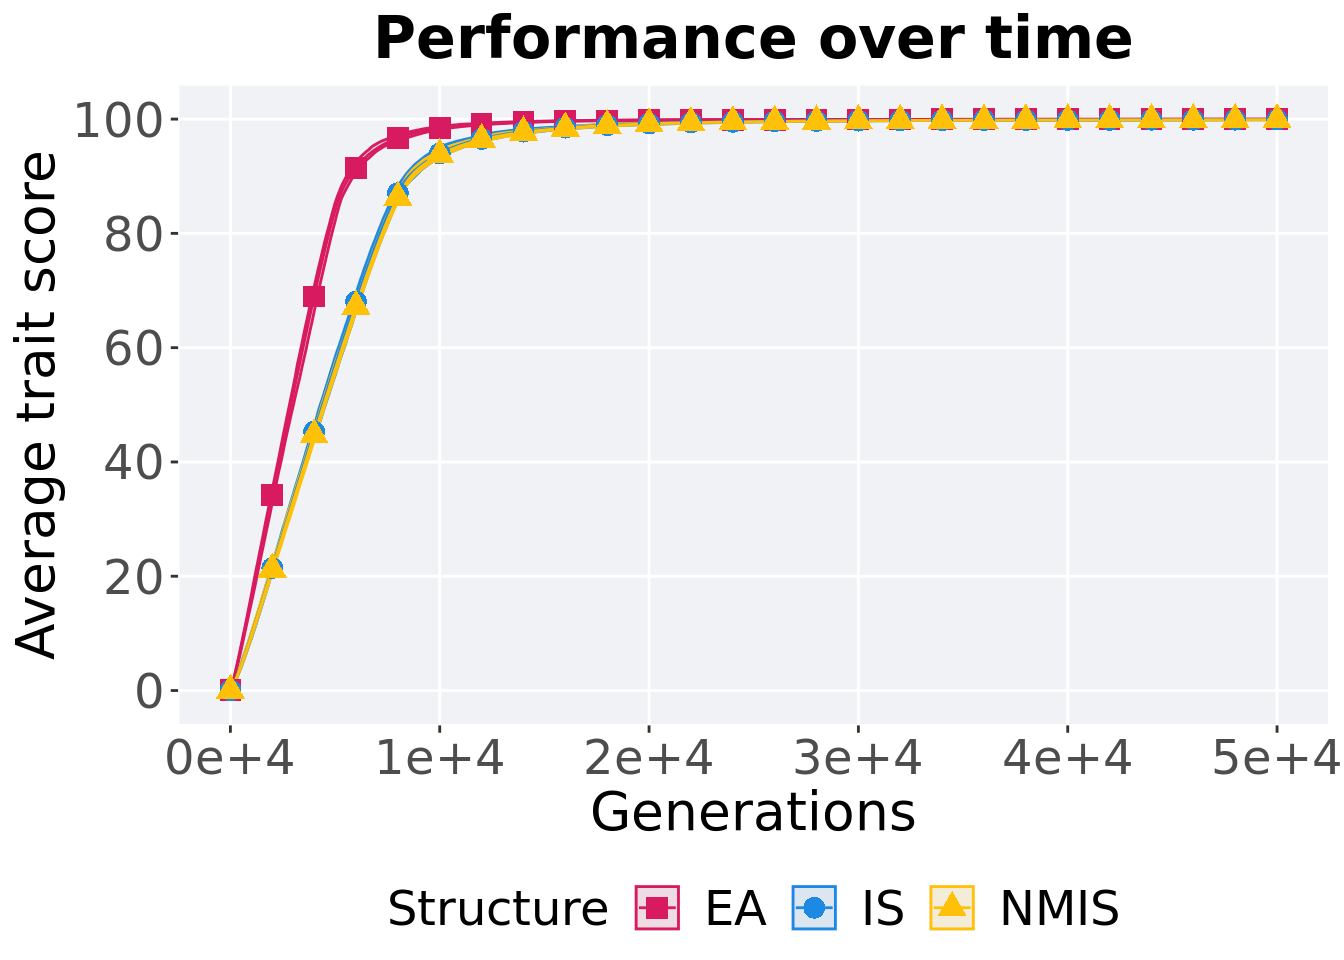
\includegraphics{demo_files/figure-latex/base-tru-ord-perf-1.pdf}

\hypertarget{generation-satisfactory-solution-found-3}{%
\subsection{Generation satisfactory solution found}\label{generation-satisfactory-solution-found-3}}

First generation a satisfactory solution is found throughout the 50,000 generations.

\begin{Shaded}
\begin{Highlighting}[]
\KeywordTok{filter}\NormalTok{(base_ssf, Diagnostic }\OperatorTok{==}\StringTok{ 'ORDERED_EXPLOITATION'} \OperatorTok{&}\StringTok{ `}\DataTypeTok{Selection}\CharTok{\textbackslash{}n}\DataTypeTok{Scheme}\StringTok{`} \OperatorTok{==}\StringTok{ 'TRUNCATION'}\NormalTok{) }\OperatorTok
\StringTok{  }\KeywordTok{ggplot}\NormalTok{(., }\KeywordTok{aes}\NormalTok{(}\DataTypeTok{x =}\NormalTok{ Structure, }\DataTypeTok{y =}\NormalTok{ Generations , }\DataTypeTok{color =}\NormalTok{ Structure, }\DataTypeTok{fill =}\NormalTok{ Structure, }\DataTypeTok{shape =}\NormalTok{ Structure)) }\OperatorTok{+}
\StringTok{  }\KeywordTok{geom_flat_violin}\NormalTok{(}\DataTypeTok{position =} \KeywordTok{position_nudge}\NormalTok{(}\DataTypeTok{x =} \FloatTok{.2}\NormalTok{, }\DataTypeTok{y =} \DecValTok{0}\NormalTok{), }\DataTypeTok{scale =} \StringTok{'width'}\NormalTok{, }\DataTypeTok{alpha =} \FloatTok{0.2}\NormalTok{) }\OperatorTok{+}
\StringTok{  }\KeywordTok{geom_point}\NormalTok{(}\DataTypeTok{position =} \KeywordTok{position_jitter}\NormalTok{(}\DataTypeTok{width =} \FloatTok{.1}\NormalTok{), }\DataTypeTok{size =} \FloatTok{1.5}\NormalTok{, }\DataTypeTok{alpha =} \FloatTok{1.0}\NormalTok{) }\OperatorTok{+}
\StringTok{  }\KeywordTok{geom_boxplot}\NormalTok{(}\DataTypeTok{color =} \StringTok{'black'}\NormalTok{, }\DataTypeTok{width =} \FloatTok{.2}\NormalTok{, }\DataTypeTok{outlier.shape =} \OtherTok{NA}\NormalTok{, }\DataTypeTok{alpha =} \FloatTok{0.0}\NormalTok{) }\OperatorTok{+}
\StringTok{  }\KeywordTok{scale_y_continuous}\NormalTok{(}
    \DataTypeTok{name=}\StringTok{"Generation"}
\NormalTok{  ) }\OperatorTok{+}
\StringTok{  }\KeywordTok{scale_x_discrete}\NormalTok{(}
    \DataTypeTok{name=}\StringTok{"Structure"}
\NormalTok{  )}\OperatorTok{+}
\StringTok{  }\KeywordTok{scale_shape_manual}\NormalTok{(}\DataTypeTok{values=}\NormalTok{SHAPE)}\OperatorTok{+}
\StringTok{  }\KeywordTok{scale_colour_manual}\NormalTok{(}\DataTypeTok{values =}\NormalTok{ cb_palette, ) }\OperatorTok{+}
\StringTok{  }\KeywordTok{scale_fill_manual}\NormalTok{(}\DataTypeTok{values =}\NormalTok{ cb_palette) }\OperatorTok{+}
\StringTok{  }\KeywordTok{ggtitle}\NormalTok{(}\StringTok{'Generation satisfactory solution found'}\NormalTok{)}\OperatorTok{+}
\StringTok{  }\NormalTok{p_theme }\OperatorTok{+}\StringTok{ }\KeywordTok{coord_flip}\NormalTok{()}
\end{Highlighting}
\end{Shaded}

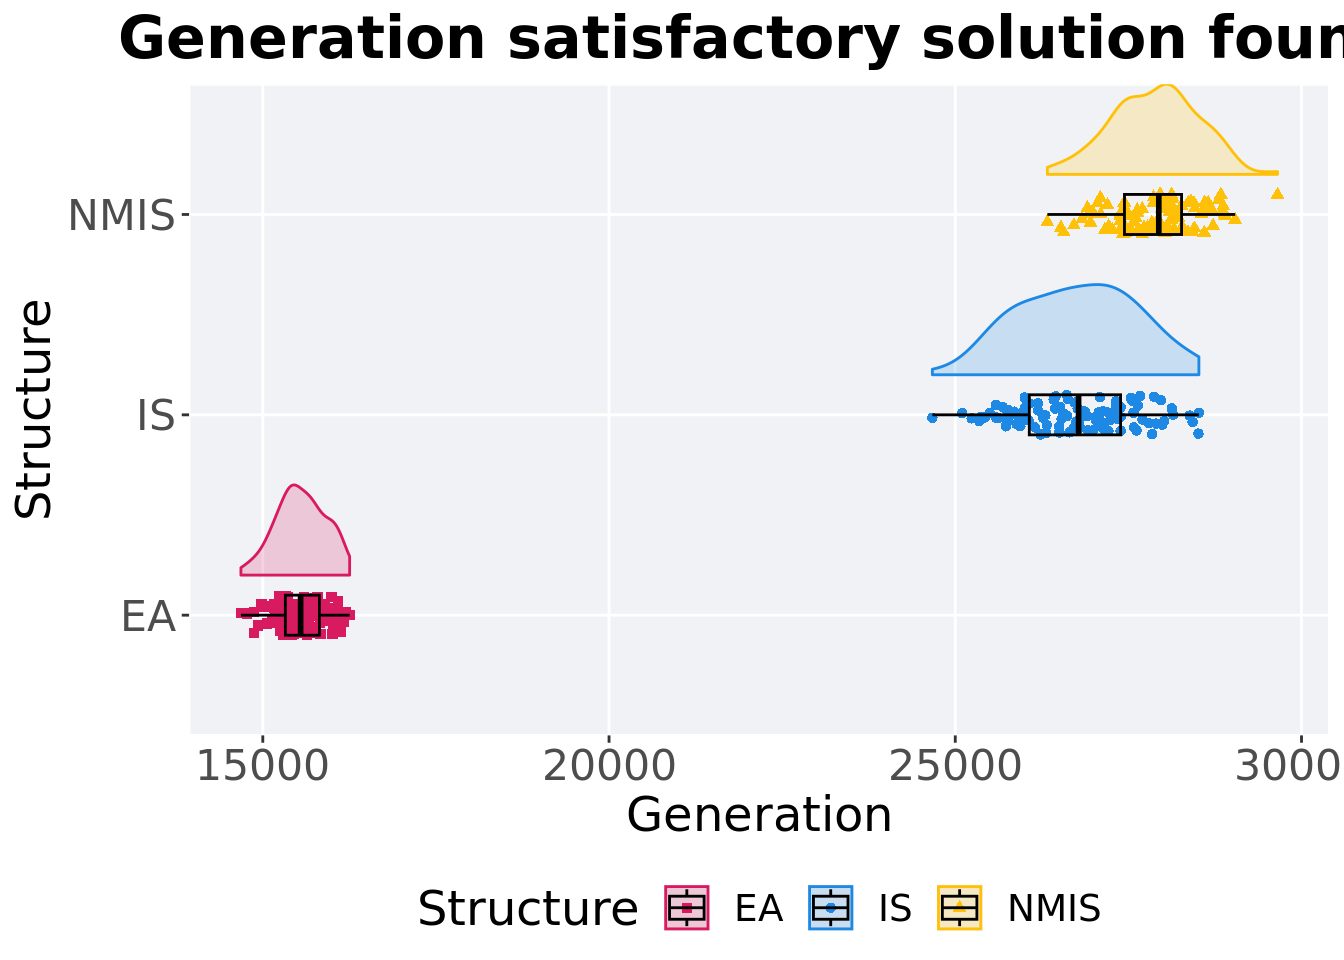
\includegraphics{demo_files/figure-latex/base-tru-ord-ssf-1.pdf}

\hypertarget{stats-3}{%
\subsubsection{Stats}\label{stats-3}}

Summary statistics for the first generation a satisfactory solution is found.

\begin{Shaded}
\begin{Highlighting}[]
\NormalTok{ssf =}\StringTok{ }\KeywordTok{filter}\NormalTok{(base_ssf, Diagnostic }\OperatorTok{==}\StringTok{ 'ORDERED_EXPLOITATION'} \OperatorTok{&}\StringTok{ `}\DataTypeTok{Selection}\CharTok{\textbackslash{}n}\DataTypeTok{Scheme}\StringTok{`} \OperatorTok{==}\StringTok{ 'TRUNCATION'} \OperatorTok{&}\StringTok{ }\NormalTok{Generations }\OperatorTok{<}\StringTok{ }\DecValTok{60000}\NormalTok{)}
\NormalTok{ssf }\OperatorTok
\StringTok{  }\KeywordTok{group_by}\NormalTok{(Structure) }\OperatorTok
\StringTok{  }\NormalTok{dplyr}\OperatorTok{::}\KeywordTok{summarise}\NormalTok{(}
    \DataTypeTok{count =} \KeywordTok{n}\NormalTok{(),}
    \DataTypeTok{na_cnt =} \KeywordTok{sum}\NormalTok{(}\KeywordTok{is.na}\NormalTok{(Generations)),}
    \DataTypeTok{min =} \KeywordTok{min}\NormalTok{(Generations, }\DataTypeTok{na.rm =} \OtherTok{TRUE}\NormalTok{),}
    \DataTypeTok{median =} \KeywordTok{median}\NormalTok{(Generations, }\DataTypeTok{na.rm =} \OtherTok{TRUE}\NormalTok{),}
    \DataTypeTok{mean =} \KeywordTok{mean}\NormalTok{(Generations, }\DataTypeTok{na.rm =} \OtherTok{TRUE}\NormalTok{),}
    \DataTypeTok{max =} \KeywordTok{max}\NormalTok{(Generations, }\DataTypeTok{na.rm =} \OtherTok{TRUE}\NormalTok{),}
    \DataTypeTok{IQR =} \KeywordTok{IQR}\NormalTok{(Generations, }\DataTypeTok{na.rm =} \OtherTok{TRUE}\NormalTok{)}
\NormalTok{  )}
\end{Highlighting}
\end{Shaded}

\begin{verbatim}
## # A tibble: 3 x 8
##   Structure count na_cnt   min median   mean   max   IQR
##   <fct>     <int>  <int> <int>  <dbl>  <dbl> <int> <dbl>
## 1 EA          100      0 14684 15546  15554. 16254  492.
## 2 IS          100      0 24669 26780. 26767. 28518 1318.
## 3 NMIS        100      0 26330 27939  27888. 29654  825.
\end{verbatim}

Kruskal--Wallis test provides evidence of difference among selection schemes.

\begin{Shaded}
\begin{Highlighting}[]
\KeywordTok{kruskal.test}\NormalTok{(Generations }\OperatorTok{~}\StringTok{ }\NormalTok{Structure, }\DataTypeTok{data =}\NormalTok{ ssf)}
\end{Highlighting}
\end{Shaded}

\begin{verbatim}
## 
##  Kruskal-Wallis rank sum test
## 
## data:  Generations by Structure
## Kruskal-Wallis chi-squared = 231.88, df = 2, p-value < 2.2e-16
\end{verbatim}

Results for post-hoc Wilcoxon rank-sum test with a Bonferroni correction.

\begin{Shaded}
\begin{Highlighting}[]
\KeywordTok{pairwise.wilcox.test}\NormalTok{(}\DataTypeTok{x =}\NormalTok{ ssf}\OperatorTok{$}\NormalTok{Generations, }\DataTypeTok{g =}\NormalTok{ ssf}\OperatorTok{$}\NormalTok{Structure, }\DataTypeTok{p.adjust.method =} \StringTok{"bonferroni"}\NormalTok{,}
                     \DataTypeTok{paired =} \OtherTok{FALSE}\NormalTok{, }\DataTypeTok{conf.int =} \OtherTok{FALSE}\NormalTok{, }\DataTypeTok{alternative =} \StringTok{'g'}\NormalTok{)}
\end{Highlighting}
\end{Shaded}

\begin{verbatim}
## 
##  Pairwise comparisons using Wilcoxon rank sum test with continuity correction 
## 
## data:  ssf$Generations and ssf$Structure 
## 
##      EA     IS    
## IS   <2e-16 -     
## NMIS <2e-16 <2e-16
## 
## P value adjustment method: bonferroni
\end{verbatim}

\hypertarget{tournament-selection-1}{%
\section{Tournament selection}\label{tournament-selection-1}}

Here we analyze how the different population structures affect tournament selection (size 8) on the ordered exploitation diagnostic.

\hypertarget{performance-over-time-4}{%
\subsection{Performance over time}\label{performance-over-time-4}}

\begin{Shaded}
\begin{Highlighting}[]
\NormalTok{lines =}\StringTok{ }\KeywordTok{filter}\NormalTok{(base_over_time, Diagnostic }\OperatorTok{==}\StringTok{ 'ORDERED_EXPLOITATION'} \OperatorTok{&}\StringTok{ `}\DataTypeTok{Selection}\CharTok{\textbackslash{}n}\DataTypeTok{Scheme}\StringTok{`} \OperatorTok{==}\StringTok{ 'TOURNAMENT'}\NormalTok{) }\OperatorTok
\StringTok{  }\KeywordTok{group_by}\NormalTok{(Structure, Generations) }\OperatorTok
\StringTok{  }\NormalTok{dplyr}\OperatorTok{::}\KeywordTok{summarise}\NormalTok{(}
    \DataTypeTok{min =} \KeywordTok{min}\NormalTok{(pop_fit_max) }\OperatorTok{/}\StringTok{ }\NormalTok{DIMENSIONALITY,}
    \DataTypeTok{mean =} \KeywordTok{mean}\NormalTok{(pop_fit_max) }\OperatorTok{/}\StringTok{ }\NormalTok{DIMENSIONALITY,}
    \DataTypeTok{max =} \KeywordTok{max}\NormalTok{(pop_fit_max) }\OperatorTok{/}\StringTok{ }\NormalTok{DIMENSIONALITY}
\NormalTok{  )}
\KeywordTok{ggplot}\NormalTok{(lines, }\KeywordTok{aes}\NormalTok{(}\DataTypeTok{x=}\NormalTok{Generations, }\DataTypeTok{y=}\NormalTok{mean, }\DataTypeTok{group =}\NormalTok{ Structure, }\DataTypeTok{fill =}\NormalTok{ Structure, }\DataTypeTok{color =}\NormalTok{ Structure, }\DataTypeTok{shape =}\NormalTok{ Structure)) }\OperatorTok{+}
\StringTok{  }\KeywordTok{geom_ribbon}\NormalTok{(}\KeywordTok{aes}\NormalTok{(}\DataTypeTok{ymin =}\NormalTok{ min, }\DataTypeTok{ymax =}\NormalTok{ max), }\DataTypeTok{alpha =} \FloatTok{0.1}\NormalTok{) }\OperatorTok{+}
\StringTok{  }\KeywordTok{geom_line}\NormalTok{(}\DataTypeTok{size =} \FloatTok{0.5}\NormalTok{) }\OperatorTok{+}
\StringTok{  }\KeywordTok{geom_point}\NormalTok{(}\DataTypeTok{data =} \KeywordTok{filter}\NormalTok{(lines, Generations }\OperatorTok\StringTok{ }\DecValTok{2000} \OperatorTok{==}\StringTok{ }\DecValTok{0}\NormalTok{), }\DataTypeTok{size =} \FloatTok{2.5}\NormalTok{, }\DataTypeTok{stroke =} \FloatTok{2.0}\NormalTok{, }\DataTypeTok{alpha =} \FloatTok{1.0}\NormalTok{) }\OperatorTok{+}
\StringTok{  }\KeywordTok{scale_y_continuous}\NormalTok{(}
    \DataTypeTok{name=}\StringTok{"Average trait score"}\NormalTok{,}
    \DataTypeTok{limits=}\KeywordTok{c}\NormalTok{(}\OperatorTok{-}\DecValTok{1}\NormalTok{, }\DecValTok{101}\NormalTok{),}
    \DataTypeTok{breaks=}\KeywordTok{seq}\NormalTok{(}\DecValTok{0}\NormalTok{,}\DecValTok{100}\NormalTok{, }\DecValTok{20}\NormalTok{),}
    \DataTypeTok{labels=}\KeywordTok{c}\NormalTok{(}\StringTok{"0"}\NormalTok{, }\StringTok{"20"}\NormalTok{, }\StringTok{"40"}\NormalTok{, }\StringTok{"60"}\NormalTok{, }\StringTok{"80"}\NormalTok{, }\StringTok{"100"}\NormalTok{)}
\NormalTok{  ) }\OperatorTok{+}
\StringTok{  }\KeywordTok{scale_x_continuous}\NormalTok{(}
    \DataTypeTok{name=}\StringTok{"Generations"}\NormalTok{,}
    \DataTypeTok{limits=}\KeywordTok{c}\NormalTok{(}\DecValTok{0}\NormalTok{, }\DecValTok{50000}\NormalTok{),}
    \DataTypeTok{breaks=}\KeywordTok{c}\NormalTok{(}\DecValTok{0}\NormalTok{, }\DecValTok{10000}\NormalTok{, }\DecValTok{20000}\NormalTok{, }\DecValTok{30000}\NormalTok{, }\DecValTok{40000}\NormalTok{, }\DecValTok{50000}\NormalTok{),}
    \DataTypeTok{labels=}\KeywordTok{c}\NormalTok{(}\StringTok{"0e+4"}\NormalTok{, }\StringTok{"1e+4"}\NormalTok{, }\StringTok{"2e+4"}\NormalTok{, }\StringTok{"3e+4"}\NormalTok{, }\StringTok{"4e+4"}\NormalTok{, }\StringTok{"5e+4"}\NormalTok{)}

\NormalTok{  ) }\OperatorTok{+}
\StringTok{  }\KeywordTok{scale_shape_manual}\NormalTok{(}\DataTypeTok{values=}\NormalTok{SHAPE)}\OperatorTok{+}
\StringTok{  }\KeywordTok{scale_colour_manual}\NormalTok{(}\DataTypeTok{values =}\NormalTok{ cb_palette) }\OperatorTok{+}
\StringTok{  }\KeywordTok{scale_fill_manual}\NormalTok{(}\DataTypeTok{values =}\NormalTok{ cb_palette) }\OperatorTok{+}
\StringTok{  }\KeywordTok{ggtitle}\NormalTok{(}\StringTok{"Performance over time"}\NormalTok{) }\OperatorTok{+}
\StringTok{  }\NormalTok{p_theme}
\end{Highlighting}
\end{Shaded}

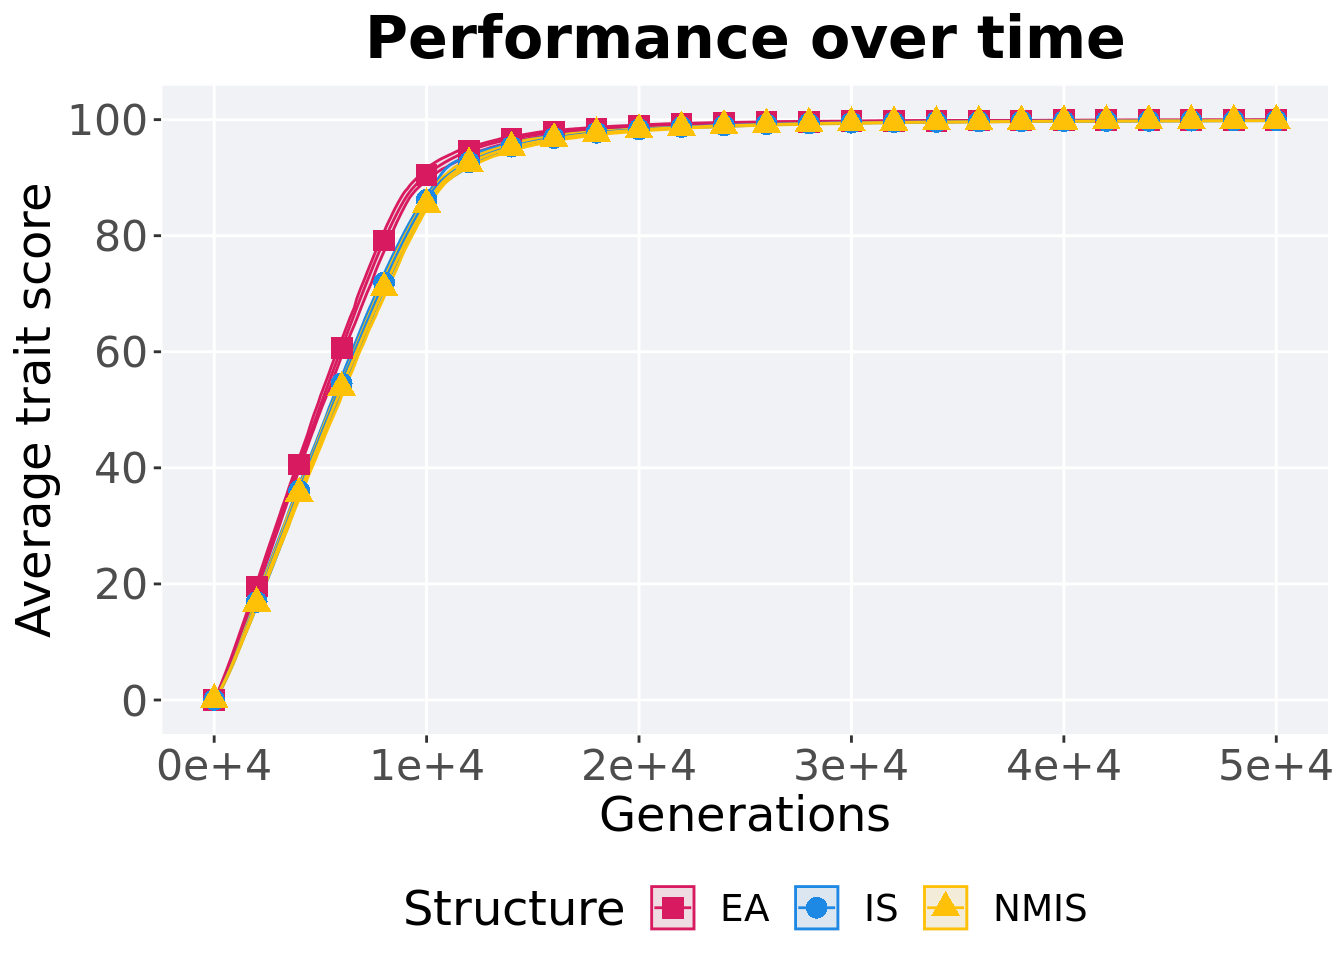
\includegraphics{demo_files/figure-latex/base-tor-ord-perf-1.pdf}

\hypertarget{generation-satisfactory-solution-found-4}{%
\subsection{Generation satisfactory solution found}\label{generation-satisfactory-solution-found-4}}

First generation a satisfactory solution is found throughout the 50,000 generations.

\begin{Shaded}
\begin{Highlighting}[]
\KeywordTok{filter}\NormalTok{(base_ssf, Diagnostic }\OperatorTok{==}\StringTok{ 'ORDERED_EXPLOITATION'} \OperatorTok{&}\StringTok{ `}\DataTypeTok{Selection}\CharTok{\textbackslash{}n}\DataTypeTok{Scheme}\StringTok{`} \OperatorTok{==}\StringTok{ 'TOURNAMENT'}\NormalTok{) }\OperatorTok
\StringTok{  }\KeywordTok{ggplot}\NormalTok{(., }\KeywordTok{aes}\NormalTok{(}\DataTypeTok{x =}\NormalTok{ Structure, }\DataTypeTok{y =}\NormalTok{ Generations , }\DataTypeTok{color =}\NormalTok{ Structure, }\DataTypeTok{fill =}\NormalTok{ Structure, }\DataTypeTok{shape =}\NormalTok{ Structure)) }\OperatorTok{+}
\StringTok{  }\KeywordTok{geom_flat_violin}\NormalTok{(}\DataTypeTok{position =} \KeywordTok{position_nudge}\NormalTok{(}\DataTypeTok{x =} \FloatTok{.2}\NormalTok{, }\DataTypeTok{y =} \DecValTok{0}\NormalTok{), }\DataTypeTok{scale =} \StringTok{'width'}\NormalTok{, }\DataTypeTok{alpha =} \FloatTok{0.2}\NormalTok{) }\OperatorTok{+}
\StringTok{  }\KeywordTok{geom_point}\NormalTok{(}\DataTypeTok{position =} \KeywordTok{position_jitter}\NormalTok{(}\DataTypeTok{width =} \FloatTok{.1}\NormalTok{), }\DataTypeTok{size =} \FloatTok{1.5}\NormalTok{, }\DataTypeTok{alpha =} \FloatTok{1.0}\NormalTok{) }\OperatorTok{+}
\StringTok{  }\KeywordTok{geom_boxplot}\NormalTok{(}\DataTypeTok{color =} \StringTok{'black'}\NormalTok{, }\DataTypeTok{width =} \FloatTok{.2}\NormalTok{, }\DataTypeTok{outlier.shape =} \OtherTok{NA}\NormalTok{, }\DataTypeTok{alpha =} \FloatTok{0.0}\NormalTok{) }\OperatorTok{+}
\StringTok{  }\KeywordTok{scale_y_continuous}\NormalTok{(}
    \DataTypeTok{name=}\StringTok{"Generation"}
\NormalTok{  ) }\OperatorTok{+}
\StringTok{  }\KeywordTok{scale_x_discrete}\NormalTok{(}
    \DataTypeTok{name=}\StringTok{"Structure"}
\NormalTok{  )}\OperatorTok{+}
\StringTok{  }\KeywordTok{scale_shape_manual}\NormalTok{(}\DataTypeTok{values=}\NormalTok{SHAPE)}\OperatorTok{+}
\StringTok{  }\KeywordTok{scale_colour_manual}\NormalTok{(}\DataTypeTok{values =}\NormalTok{ cb_palette, ) }\OperatorTok{+}
\StringTok{  }\KeywordTok{scale_fill_manual}\NormalTok{(}\DataTypeTok{values =}\NormalTok{ cb_palette) }\OperatorTok{+}
\StringTok{  }\KeywordTok{ggtitle}\NormalTok{(}\StringTok{'Generation satisfactory solution found'}\NormalTok{)}\OperatorTok{+}
\StringTok{  }\NormalTok{p_theme }\OperatorTok{+}\StringTok{ }\KeywordTok{coord_flip}\NormalTok{()}
\end{Highlighting}
\end{Shaded}

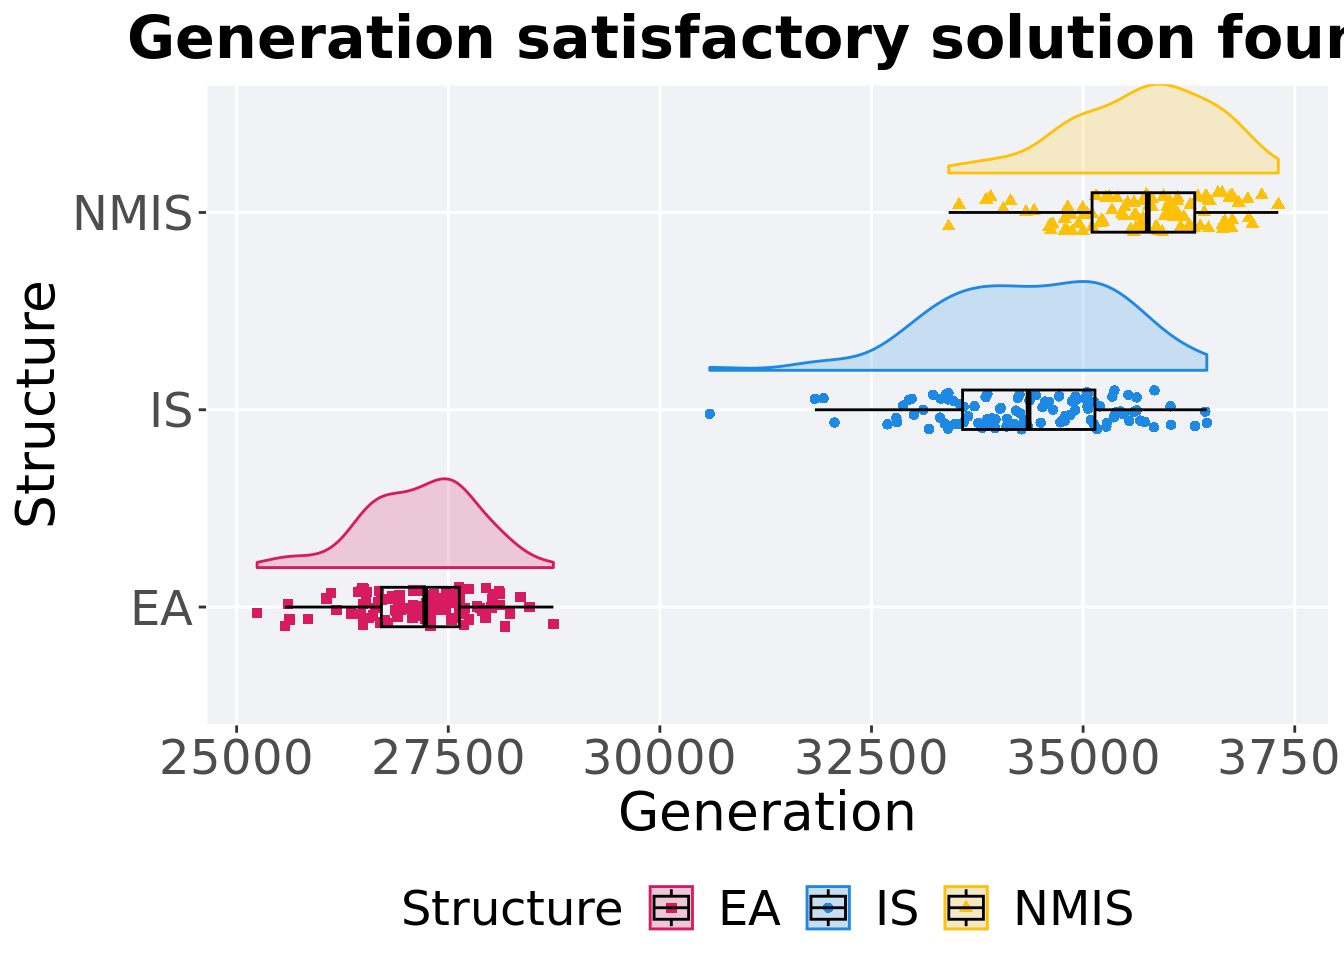
\includegraphics{demo_files/figure-latex/base-tor-ord-ssf-1.pdf}

\hypertarget{stats-4}{%
\subsubsection{Stats}\label{stats-4}}

Summary statistics for the first generation a satisfactory solution is found.

\begin{Shaded}
\begin{Highlighting}[]
\NormalTok{ssf =}\StringTok{ }\KeywordTok{filter}\NormalTok{(base_ssf, Diagnostic }\OperatorTok{==}\StringTok{ 'ORDERED_EXPLOITATION'} \OperatorTok{&}\StringTok{ `}\DataTypeTok{Selection}\CharTok{\textbackslash{}n}\DataTypeTok{Scheme}\StringTok{`} \OperatorTok{==}\StringTok{ 'TOURNAMENT'} \OperatorTok{&}\StringTok{ }\NormalTok{Generations }\OperatorTok{<}\StringTok{ }\DecValTok{60000}\NormalTok{)}
\NormalTok{ssf }\OperatorTok
\StringTok{  }\KeywordTok{group_by}\NormalTok{(Structure) }\OperatorTok
\StringTok{  }\NormalTok{dplyr}\OperatorTok{::}\KeywordTok{summarise}\NormalTok{(}
    \DataTypeTok{count =} \KeywordTok{n}\NormalTok{(),}
    \DataTypeTok{na_cnt =} \KeywordTok{sum}\NormalTok{(}\KeywordTok{is.na}\NormalTok{(Generations)),}
    \DataTypeTok{min =} \KeywordTok{min}\NormalTok{(Generations, }\DataTypeTok{na.rm =} \OtherTok{TRUE}\NormalTok{),}
    \DataTypeTok{median =} \KeywordTok{median}\NormalTok{(Generations, }\DataTypeTok{na.rm =} \OtherTok{TRUE}\NormalTok{),}
    \DataTypeTok{mean =} \KeywordTok{mean}\NormalTok{(Generations, }\DataTypeTok{na.rm =} \OtherTok{TRUE}\NormalTok{),}
    \DataTypeTok{max =} \KeywordTok{max}\NormalTok{(Generations, }\DataTypeTok{na.rm =} \OtherTok{TRUE}\NormalTok{),}
    \DataTypeTok{IQR =} \KeywordTok{IQR}\NormalTok{(Generations, }\DataTypeTok{na.rm =} \OtherTok{TRUE}\NormalTok{)}
\NormalTok{  )}
\end{Highlighting}
\end{Shaded}

\begin{verbatim}
## # A tibble: 3 x 8
##   Structure count na_cnt   min median   mean   max   IQR
##   <fct>     <int>  <int> <int>  <dbl>  <dbl> <int> <dbl>
## 1 EA          100      0 25242 27228. 27172. 28742  921.
## 2 IS          100      0 30589 34356. 34349. 36461 1564.
## 3 NMIS        100      0 33412 35764  35692. 37306 1213
\end{verbatim}

Kruskal--Wallis test provides evidence of difference among selection schemes.

\begin{Shaded}
\begin{Highlighting}[]
\KeywordTok{kruskal.test}\NormalTok{(Generations }\OperatorTok{~}\StringTok{ }\NormalTok{Structure, }\DataTypeTok{data =}\NormalTok{ ssf)}
\end{Highlighting}
\end{Shaded}

\begin{verbatim}
## 
##  Kruskal-Wallis rank sum test
## 
## data:  Generations by Structure
## Kruskal-Wallis chi-squared = 229.49, df = 2, p-value < 2.2e-16
\end{verbatim}

Results for post-hoc Wilcoxon rank-sum test with a Bonferroni correction.

\begin{Shaded}
\begin{Highlighting}[]
\KeywordTok{pairwise.wilcox.test}\NormalTok{(}\DataTypeTok{x =}\NormalTok{ ssf}\OperatorTok{$}\NormalTok{Generations, }\DataTypeTok{g =}\NormalTok{ ssf}\OperatorTok{$}\NormalTok{Structure, }\DataTypeTok{p.adjust.method =} \StringTok{"bonferroni"}\NormalTok{,}
                     \DataTypeTok{paired =} \OtherTok{FALSE}\NormalTok{, }\DataTypeTok{conf.int =} \OtherTok{FALSE}\NormalTok{, }\DataTypeTok{alternative =} \StringTok{'g'}\NormalTok{)}
\end{Highlighting}
\end{Shaded}

\begin{verbatim}
## 
##  Pairwise comparisons using Wilcoxon rank sum test with continuity correction 
## 
## data:  ssf$Generations and ssf$Structure 
## 
##      EA      IS     
## IS   < 2e-16 -      
## NMIS < 2e-16 2.8e-16
## 
## P value adjustment method: bonferroni
\end{verbatim}

\hypertarget{lexicase-selection-1}{%
\section{Lexicase selection}\label{lexicase-selection-1}}

Here we analyze how the different population structures affect standard lexicase selection on the ordered exploitation diagnostic.

\hypertarget{performance-over-time-5}{%
\subsection{Performance over time}\label{performance-over-time-5}}

\begin{Shaded}
\begin{Highlighting}[]
\NormalTok{lines =}\StringTok{ }\KeywordTok{filter}\NormalTok{(base_over_time, Diagnostic }\OperatorTok{==}\StringTok{ 'ORDERED_EXPLOITATION'} \OperatorTok{&}\StringTok{ `}\DataTypeTok{Selection}\CharTok{\textbackslash{}n}\DataTypeTok{Scheme}\StringTok{`} \OperatorTok{==}\StringTok{ 'LEXICASE'}\NormalTok{) }\OperatorTok
\StringTok{  }\KeywordTok{group_by}\NormalTok{(Structure, Generations) }\OperatorTok
\StringTok{  }\NormalTok{dplyr}\OperatorTok{::}\KeywordTok{summarise}\NormalTok{(}
    \DataTypeTok{min =} \KeywordTok{min}\NormalTok{(pop_fit_max) }\OperatorTok{/}\StringTok{ }\NormalTok{DIMENSIONALITY,}
    \DataTypeTok{mean =} \KeywordTok{mean}\NormalTok{(pop_fit_max) }\OperatorTok{/}\StringTok{ }\NormalTok{DIMENSIONALITY,}
    \DataTypeTok{max =} \KeywordTok{max}\NormalTok{(pop_fit_max) }\OperatorTok{/}\StringTok{ }\NormalTok{DIMENSIONALITY}
\NormalTok{  )}
\KeywordTok{ggplot}\NormalTok{(lines, }\KeywordTok{aes}\NormalTok{(}\DataTypeTok{x=}\NormalTok{Generations, }\DataTypeTok{y=}\NormalTok{mean, }\DataTypeTok{group =}\NormalTok{ Structure, }\DataTypeTok{fill =}\NormalTok{ Structure, }\DataTypeTok{color =}\NormalTok{ Structure, }\DataTypeTok{shape =}\NormalTok{ Structure)) }\OperatorTok{+}
\StringTok{  }\KeywordTok{geom_ribbon}\NormalTok{(}\KeywordTok{aes}\NormalTok{(}\DataTypeTok{ymin =}\NormalTok{ min, }\DataTypeTok{ymax =}\NormalTok{ max), }\DataTypeTok{alpha =} \FloatTok{0.1}\NormalTok{) }\OperatorTok{+}
\StringTok{  }\KeywordTok{geom_line}\NormalTok{(}\DataTypeTok{size =} \FloatTok{0.5}\NormalTok{) }\OperatorTok{+}
\StringTok{  }\KeywordTok{geom_point}\NormalTok{(}\DataTypeTok{data =} \KeywordTok{filter}\NormalTok{(lines, Generations }\OperatorTok\StringTok{ }\DecValTok{2000} \OperatorTok{==}\StringTok{ }\DecValTok{0}\NormalTok{), }\DataTypeTok{size =} \FloatTok{2.5}\NormalTok{, }\DataTypeTok{stroke =} \FloatTok{2.0}\NormalTok{, }\DataTypeTok{alpha =} \FloatTok{1.0}\NormalTok{) }\OperatorTok{+}
\StringTok{  }\KeywordTok{scale_y_continuous}\NormalTok{(}
    \DataTypeTok{name=}\StringTok{"Average trait score"}\NormalTok{,}
    \DataTypeTok{limits=}\KeywordTok{c}\NormalTok{(}\OperatorTok{-}\DecValTok{1}\NormalTok{, }\DecValTok{101}\NormalTok{),}
    \DataTypeTok{breaks=}\KeywordTok{seq}\NormalTok{(}\DecValTok{0}\NormalTok{,}\DecValTok{100}\NormalTok{, }\DecValTok{20}\NormalTok{),}
    \DataTypeTok{labels=}\KeywordTok{c}\NormalTok{(}\StringTok{"0"}\NormalTok{, }\StringTok{"20"}\NormalTok{, }\StringTok{"40"}\NormalTok{, }\StringTok{"60"}\NormalTok{, }\StringTok{"80"}\NormalTok{, }\StringTok{"100"}\NormalTok{)}
\NormalTok{  ) }\OperatorTok{+}
\StringTok{  }\KeywordTok{scale_x_continuous}\NormalTok{(}
    \DataTypeTok{name=}\StringTok{"Generations"}\NormalTok{,}
    \DataTypeTok{limits=}\KeywordTok{c}\NormalTok{(}\DecValTok{0}\NormalTok{, }\DecValTok{50000}\NormalTok{),}
    \DataTypeTok{breaks=}\KeywordTok{c}\NormalTok{(}\DecValTok{0}\NormalTok{, }\DecValTok{10000}\NormalTok{, }\DecValTok{20000}\NormalTok{, }\DecValTok{30000}\NormalTok{, }\DecValTok{40000}\NormalTok{, }\DecValTok{50000}\NormalTok{),}
    \DataTypeTok{labels=}\KeywordTok{c}\NormalTok{(}\StringTok{"0e+4"}\NormalTok{, }\StringTok{"1e+4"}\NormalTok{, }\StringTok{"2e+4"}\NormalTok{, }\StringTok{"3e+4"}\NormalTok{, }\StringTok{"4e+4"}\NormalTok{, }\StringTok{"5e+4"}\NormalTok{)}

\NormalTok{  ) }\OperatorTok{+}
\StringTok{  }\KeywordTok{scale_shape_manual}\NormalTok{(}\DataTypeTok{values=}\NormalTok{SHAPE)}\OperatorTok{+}
\StringTok{  }\KeywordTok{scale_colour_manual}\NormalTok{(}\DataTypeTok{values =}\NormalTok{ cb_palette) }\OperatorTok{+}
\StringTok{  }\KeywordTok{scale_fill_manual}\NormalTok{(}\DataTypeTok{values =}\NormalTok{ cb_palette) }\OperatorTok{+}
\StringTok{  }\KeywordTok{ggtitle}\NormalTok{(}\StringTok{"Performance over time"}\NormalTok{) }\OperatorTok{+}
\StringTok{  }\NormalTok{p_theme}
\end{Highlighting}
\end{Shaded}

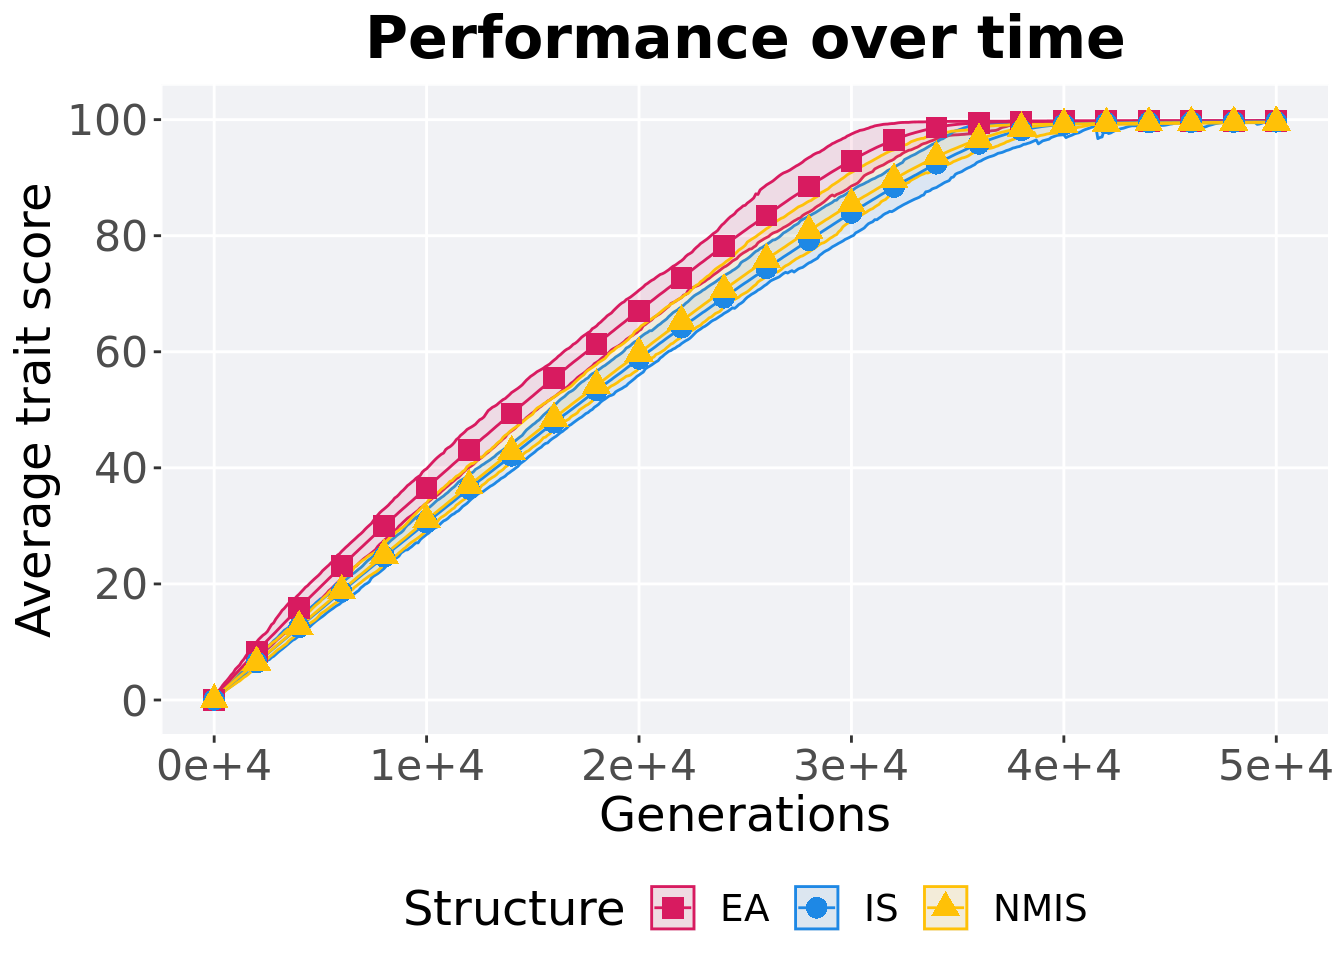
\includegraphics{demo_files/figure-latex/base-lex-ord-perf-1.pdf}

\hypertarget{best-performance}{%
\subsection{Best performance}\label{best-performance}}

First generation a satisfactory solution is found throughout the 50,000 generations.

\begin{Shaded}
\begin{Highlighting}[]
\KeywordTok{filter}\NormalTok{(base_best, Diagnostic }\OperatorTok{==}\StringTok{ 'ORDERED_EXPLOITATION'} \OperatorTok{&}\StringTok{ `}\DataTypeTok{Selection}\CharTok{\textbackslash{}n}\DataTypeTok{Scheme}\StringTok{`} \OperatorTok{==}\StringTok{ 'LEXICASE'} \OperatorTok{&}\StringTok{ }\NormalTok{VAR }\OperatorTok{==}\StringTok{ 'pop_fit_max'}\NormalTok{) }\OperatorTok
\StringTok{  }\KeywordTok{ggplot}\NormalTok{(., }\KeywordTok{aes}\NormalTok{(}\DataTypeTok{x =}\NormalTok{ Structure, }\DataTypeTok{y =}\NormalTok{ VAL }\OperatorTok{/}\StringTok{ }\NormalTok{DIMENSIONALITY, }\DataTypeTok{color =}\NormalTok{ Structure, }\DataTypeTok{fill =}\NormalTok{ Structure, }\DataTypeTok{shape =}\NormalTok{ Structure)) }\OperatorTok{+}
\StringTok{  }\KeywordTok{geom_flat_violin}\NormalTok{(}\DataTypeTok{position =} \KeywordTok{position_nudge}\NormalTok{(}\DataTypeTok{x =} \FloatTok{.2}\NormalTok{, }\DataTypeTok{y =} \DecValTok{0}\NormalTok{), }\DataTypeTok{scale =} \StringTok{'width'}\NormalTok{, }\DataTypeTok{alpha =} \FloatTok{0.2}\NormalTok{) }\OperatorTok{+}
\StringTok{  }\KeywordTok{geom_point}\NormalTok{(}\DataTypeTok{position =} \KeywordTok{position_jitter}\NormalTok{(}\DataTypeTok{width =} \FloatTok{.1}\NormalTok{), }\DataTypeTok{size =} \FloatTok{1.5}\NormalTok{, }\DataTypeTok{alpha =} \FloatTok{1.0}\NormalTok{) }\OperatorTok{+}
\StringTok{  }\KeywordTok{geom_boxplot}\NormalTok{(}\DataTypeTok{color =} \StringTok{'black'}\NormalTok{, }\DataTypeTok{width =} \FloatTok{.2}\NormalTok{, }\DataTypeTok{outlier.shape =} \OtherTok{NA}\NormalTok{, }\DataTypeTok{alpha =} \FloatTok{0.0}\NormalTok{) }\OperatorTok{+}
\StringTok{  }\KeywordTok{scale_y_continuous}\NormalTok{(}
    \DataTypeTok{name=}\StringTok{"Average trait score"}
\NormalTok{  ) }\OperatorTok{+}
\StringTok{  }\KeywordTok{scale_x_discrete}\NormalTok{(}
    \DataTypeTok{name=}\StringTok{"Structure"}
\NormalTok{  )}\OperatorTok{+}
\StringTok{  }\KeywordTok{scale_shape_manual}\NormalTok{(}\DataTypeTok{values=}\NormalTok{SHAPE)}\OperatorTok{+}
\StringTok{  }\KeywordTok{scale_colour_manual}\NormalTok{(}\DataTypeTok{values =}\NormalTok{ cb_palette, ) }\OperatorTok{+}
\StringTok{  }\KeywordTok{scale_fill_manual}\NormalTok{(}\DataTypeTok{values =}\NormalTok{ cb_palette) }\OperatorTok{+}
\StringTok{  }\KeywordTok{ggtitle}\NormalTok{(}\StringTok{'Best performance'}\NormalTok{)}\OperatorTok{+}
\StringTok{  }\NormalTok{p_theme }\OperatorTok{+}\StringTok{ }\KeywordTok{coord_flip}\NormalTok{()}
\end{Highlighting}
\end{Shaded}

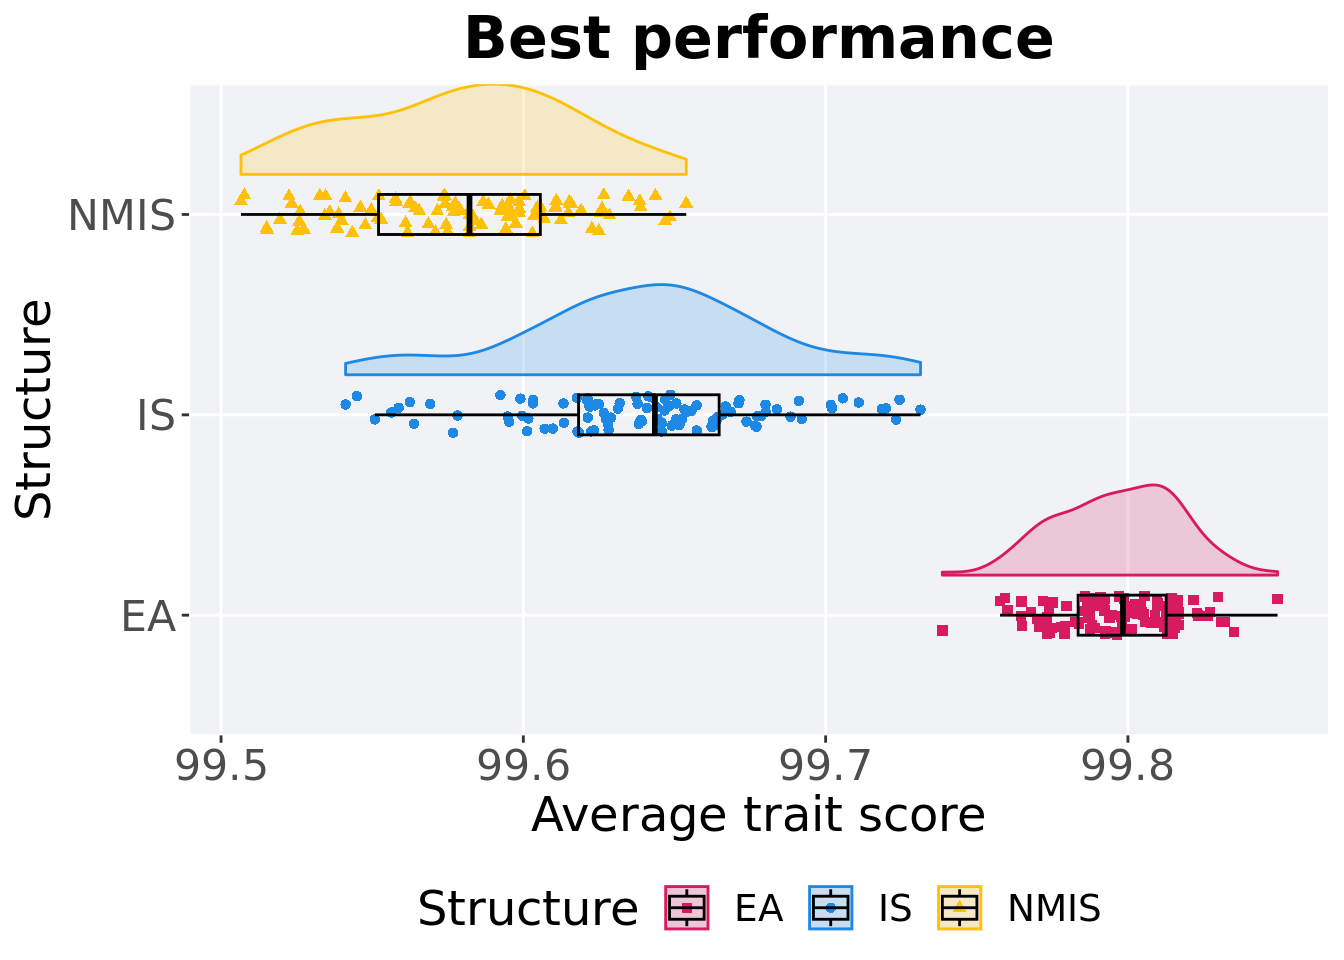
\includegraphics{demo_files/figure-latex/base-lex-ord-per-bst-1.pdf}

\hypertarget{stats-5}{%
\subsubsection{Stats}\label{stats-5}}

Summary statistics for the first generation a satisfactory solution is found.

\begin{Shaded}
\begin{Highlighting}[]
\NormalTok{performance =}\StringTok{ }\KeywordTok{filter}\NormalTok{(base_best, Diagnostic }\OperatorTok{==}\StringTok{ 'ORDERED_EXPLOITATION'} \OperatorTok{&}\StringTok{ `}\DataTypeTok{Selection}\CharTok{\textbackslash{}n}\DataTypeTok{Scheme}\StringTok{`} \OperatorTok{==}\StringTok{ 'LEXICASE'} \OperatorTok{&}\StringTok{ }\NormalTok{VAR }\OperatorTok{==}\StringTok{ 'pop_fit_max'}\NormalTok{)}
\NormalTok{performance }\OperatorTok
\StringTok{  }\KeywordTok{group_by}\NormalTok{(Structure) }\OperatorTok
\StringTok{  }\NormalTok{dplyr}\OperatorTok{::}\KeywordTok{summarise}\NormalTok{(}
    \DataTypeTok{count =} \KeywordTok{n}\NormalTok{(),}
    \DataTypeTok{na_cnt =} \KeywordTok{sum}\NormalTok{(}\KeywordTok{is.na}\NormalTok{(VAL)),}
    \DataTypeTok{min =} \KeywordTok{min}\NormalTok{(VAL, }\DataTypeTok{na.rm =} \OtherTok{TRUE}\NormalTok{) }\OperatorTok{/}\StringTok{ }\NormalTok{DIMENSIONALITY,}
    \DataTypeTok{median =} \KeywordTok{median}\NormalTok{(VAL, }\DataTypeTok{na.rm =} \OtherTok{TRUE}\NormalTok{) }\OperatorTok{/}\StringTok{ }\NormalTok{DIMENSIONALITY,}
    \DataTypeTok{mean =} \KeywordTok{mean}\NormalTok{(VAL, }\DataTypeTok{na.rm =} \OtherTok{TRUE}\NormalTok{) }\OperatorTok{/}\StringTok{ }\NormalTok{DIMENSIONALITY,}
    \DataTypeTok{max =} \KeywordTok{max}\NormalTok{(VAL, }\DataTypeTok{na.rm =} \OtherTok{TRUE}\NormalTok{) }\OperatorTok{/}\StringTok{ }\NormalTok{DIMENSIONALITY,}
    \DataTypeTok{IQR =} \KeywordTok{IQR}\NormalTok{(VAL, }\DataTypeTok{na.rm =} \OtherTok{TRUE}\NormalTok{) }\OperatorTok{/}\StringTok{ }\NormalTok{DIMENSIONALITY}
\NormalTok{  )}
\end{Highlighting}
\end{Shaded}

\begin{verbatim}
## # A tibble: 3 x 8
##   Structure count na_cnt   min median  mean   max    IQR
##   <fct>     <int>  <int> <dbl>  <dbl> <dbl> <dbl>  <dbl>
## 1 EA          100      0  99.7   99.8  99.8  99.8 0.0291
## 2 IS          100      0  99.5   99.6  99.6  99.7 0.0465
## 3 NMIS        100      0  99.5   99.6  99.6  99.7 0.0535
\end{verbatim}

Kruskal--Wallis test provides evidence of difference among selection schemes.

\begin{Shaded}
\begin{Highlighting}[]
\KeywordTok{kruskal.test}\NormalTok{(VAL }\OperatorTok{~}\StringTok{ }\NormalTok{Structure, }\DataTypeTok{data =}\NormalTok{ performance)}
\end{Highlighting}
\end{Shaded}

\begin{verbatim}
## 
##  Kruskal-Wallis rank sum test
## 
## data:  VAL by Structure
## Kruskal-Wallis chi-squared = 235.04, df = 2, p-value < 2.2e-16
\end{verbatim}

Results for post-hoc Wilcoxon rank-sum test with a Bonferroni correction.

\begin{Shaded}
\begin{Highlighting}[]
\KeywordTok{pairwise.wilcox.test}\NormalTok{(}\DataTypeTok{x =}\NormalTok{ performance}\OperatorTok{$}\NormalTok{VAL, }\DataTypeTok{g =}\NormalTok{ performance}\OperatorTok{$}\NormalTok{Structure, }\DataTypeTok{p.adjust.method =} \StringTok{"bonferroni"}\NormalTok{,}
                     \DataTypeTok{paired =} \OtherTok{FALSE}\NormalTok{, }\DataTypeTok{conf.int =} \OtherTok{FALSE}\NormalTok{, }\DataTypeTok{alternative =} \StringTok{'l'}\NormalTok{)}
\end{Highlighting}
\end{Shaded}

\begin{verbatim}
## 
##  Pairwise comparisons using Wilcoxon rank sum test with continuity correction 
## 
## data:  performance$VAL and performance$Structure 
## 
##      EA     IS    
## IS   <2e-16 -     
## NMIS <2e-16 <2e-16
## 
## P value adjustment method: bonferroni
\end{verbatim}

\hypertarget{final-performance}{%
\subsection{Final performance}\label{final-performance}}

First generation a satisfactory solution is found throughout the 50,000 generations.

\begin{Shaded}
\begin{Highlighting}[]
\KeywordTok{filter}\NormalTok{(base_over_time, Diagnostic }\OperatorTok{==}\StringTok{ 'ORDERED_EXPLOITATION'} \OperatorTok{&}\StringTok{ `}\DataTypeTok{Selection}\CharTok{\textbackslash{}n}\DataTypeTok{Scheme}\StringTok{`} \OperatorTok{==}\StringTok{ 'LEXICASE'} \OperatorTok{&}\StringTok{ }\NormalTok{Generations }\OperatorTok{==}\StringTok{ }\DecValTok{50000}\NormalTok{) }\OperatorTok
\StringTok{  }\KeywordTok{ggplot}\NormalTok{(., }\KeywordTok{aes}\NormalTok{(}\DataTypeTok{x =}\NormalTok{ Structure, }\DataTypeTok{y =}\NormalTok{ pop_fit_max }\OperatorTok{/}\StringTok{ }\NormalTok{DIMENSIONALITY, }\DataTypeTok{color =}\NormalTok{ Structure, }\DataTypeTok{fill =}\NormalTok{ Structure, }\DataTypeTok{shape =}\NormalTok{ Structure)) }\OperatorTok{+}
\StringTok{  }\KeywordTok{geom_flat_violin}\NormalTok{(}\DataTypeTok{position =} \KeywordTok{position_nudge}\NormalTok{(}\DataTypeTok{x =} \FloatTok{.2}\NormalTok{, }\DataTypeTok{y =} \DecValTok{0}\NormalTok{), }\DataTypeTok{scale =} \StringTok{'width'}\NormalTok{, }\DataTypeTok{alpha =} \FloatTok{0.2}\NormalTok{) }\OperatorTok{+}
\StringTok{  }\KeywordTok{geom_point}\NormalTok{(}\DataTypeTok{position =} \KeywordTok{position_jitter}\NormalTok{(}\DataTypeTok{width =} \FloatTok{.1}\NormalTok{), }\DataTypeTok{size =} \FloatTok{1.5}\NormalTok{, }\DataTypeTok{alpha =} \FloatTok{1.0}\NormalTok{) }\OperatorTok{+}
\StringTok{  }\KeywordTok{geom_boxplot}\NormalTok{(}\DataTypeTok{color =} \StringTok{'black'}\NormalTok{, }\DataTypeTok{width =} \FloatTok{.2}\NormalTok{, }\DataTypeTok{outlier.shape =} \OtherTok{NA}\NormalTok{, }\DataTypeTok{alpha =} \FloatTok{0.0}\NormalTok{) }\OperatorTok{+}
\StringTok{  }\KeywordTok{scale_y_continuous}\NormalTok{(}
    \DataTypeTok{name=}\StringTok{"Average trait score"}
\NormalTok{  ) }\OperatorTok{+}
\StringTok{  }\KeywordTok{scale_x_discrete}\NormalTok{(}
    \DataTypeTok{name=}\StringTok{"Structure"}
\NormalTok{  )}\OperatorTok{+}
\StringTok{  }\KeywordTok{scale_shape_manual}\NormalTok{(}\DataTypeTok{values=}\NormalTok{SHAPE)}\OperatorTok{+}
\StringTok{  }\KeywordTok{scale_colour_manual}\NormalTok{(}\DataTypeTok{values =}\NormalTok{ cb_palette, ) }\OperatorTok{+}
\StringTok{  }\KeywordTok{scale_fill_manual}\NormalTok{(}\DataTypeTok{values =}\NormalTok{ cb_palette) }\OperatorTok{+}
\StringTok{  }\KeywordTok{ggtitle}\NormalTok{(}\StringTok{'Final performance'}\NormalTok{)}\OperatorTok{+}
\StringTok{  }\NormalTok{p_theme }\OperatorTok{+}\StringTok{ }\KeywordTok{coord_flip}\NormalTok{()}
\end{Highlighting}
\end{Shaded}

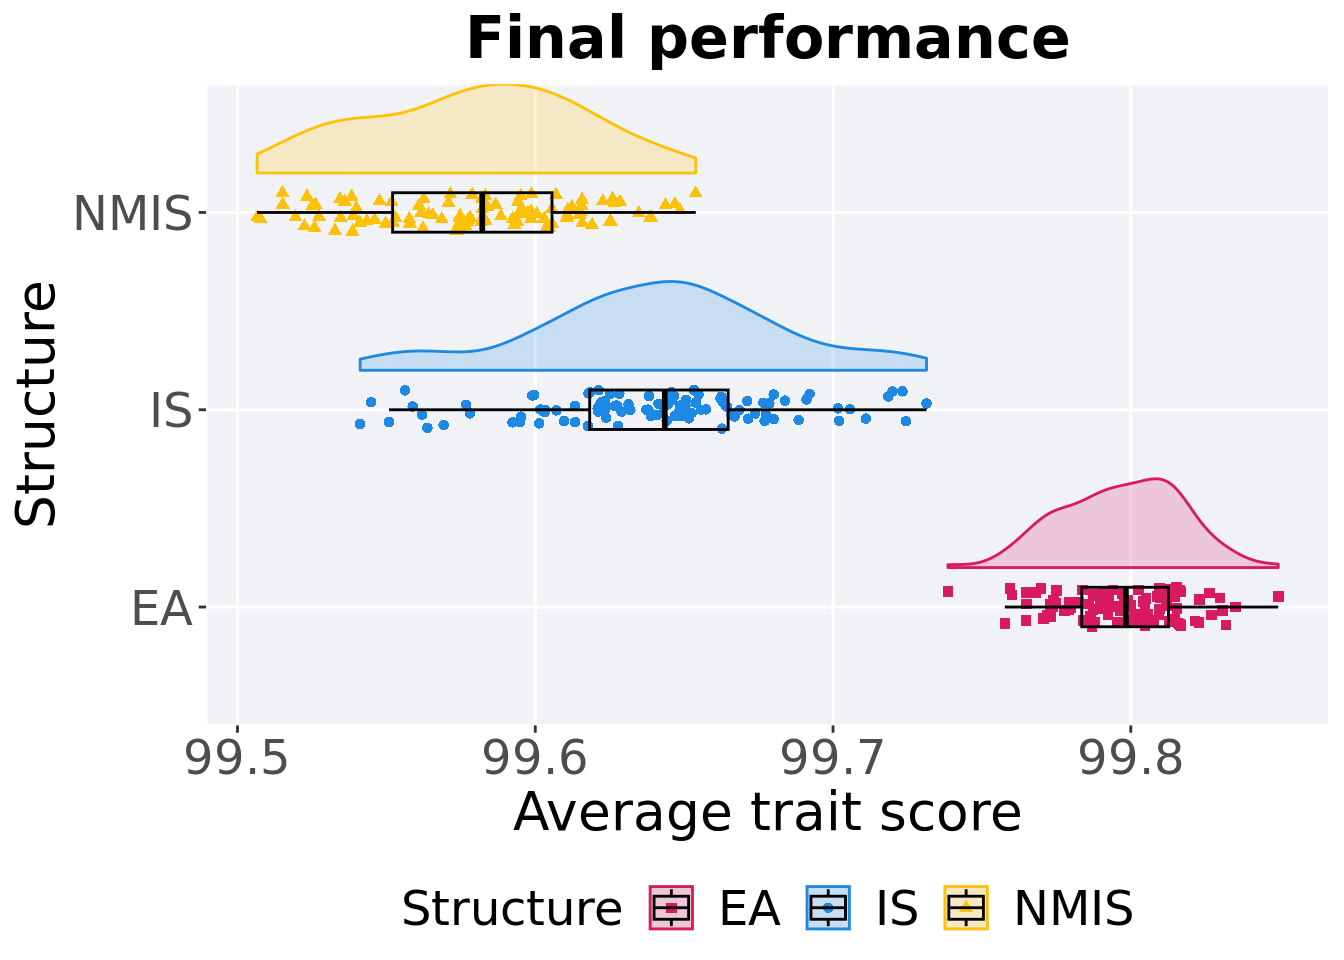
\includegraphics{demo_files/figure-latex/base-tor-ord-per-end-1.pdf}

\hypertarget{stats-6}{%
\subsubsection{Stats}\label{stats-6}}

Summary statistics for the first generation a satisfactory solution is found.

\begin{Shaded}
\begin{Highlighting}[]
\NormalTok{performance =}\StringTok{ }\KeywordTok{filter}\NormalTok{(base_over_time, Diagnostic }\OperatorTok{==}\StringTok{ 'ORDERED_EXPLOITATION'} \OperatorTok{&}\StringTok{ `}\DataTypeTok{Selection}\CharTok{\textbackslash{}n}\DataTypeTok{Scheme}\StringTok{`} \OperatorTok{==}\StringTok{ 'LEXICASE'} \OperatorTok{&}\StringTok{ }\NormalTok{Generations }\OperatorTok{==}\StringTok{ }\DecValTok{50000}\NormalTok{)}
\NormalTok{performance }\OperatorTok
\StringTok{  }\KeywordTok{group_by}\NormalTok{(Structure) }\OperatorTok
\StringTok{  }\NormalTok{dplyr}\OperatorTok{::}\KeywordTok{summarise}\NormalTok{(}
    \DataTypeTok{count =} \KeywordTok{n}\NormalTok{(),}
    \DataTypeTok{na_cnt =} \KeywordTok{sum}\NormalTok{(}\KeywordTok{is.na}\NormalTok{(pop_fit_max)),}
    \DataTypeTok{min =} \KeywordTok{min}\NormalTok{(pop_fit_max }\OperatorTok{/}\StringTok{ }\NormalTok{DIMENSIONALITY, }\DataTypeTok{na.rm =} \OtherTok{TRUE}\NormalTok{),}
    \DataTypeTok{median =} \KeywordTok{median}\NormalTok{(pop_fit_max }\OperatorTok{/}\StringTok{ }\NormalTok{DIMENSIONALITY, }\DataTypeTok{na.rm =} \OtherTok{TRUE}\NormalTok{),}
    \DataTypeTok{mean =} \KeywordTok{mean}\NormalTok{(pop_fit_max }\OperatorTok{/}\StringTok{ }\NormalTok{DIMENSIONALITY, }\DataTypeTok{na.rm =} \OtherTok{TRUE}\NormalTok{),}
    \DataTypeTok{max =} \KeywordTok{max}\NormalTok{(pop_fit_max }\OperatorTok{/}\StringTok{ }\NormalTok{DIMENSIONALITY, }\DataTypeTok{na.rm =} \OtherTok{TRUE}\NormalTok{),}
    \DataTypeTok{IQR =} \KeywordTok{IQR}\NormalTok{(pop_fit_max }\OperatorTok{/}\StringTok{ }\NormalTok{DIMENSIONALITY, }\DataTypeTok{na.rm =} \OtherTok{TRUE}\NormalTok{)}
\NormalTok{  )}
\end{Highlighting}
\end{Shaded}

\begin{verbatim}
## # A tibble: 3 x 8
##   Structure count na_cnt   min median  mean   max    IQR
##   <fct>     <int>  <int> <dbl>  <dbl> <dbl> <dbl>  <dbl>
## 1 EA          100      0  99.7   99.8  99.8  99.8 0.0291
## 2 IS          100      0  99.5   99.6  99.6  99.7 0.0465
## 3 NMIS        100      0  99.5   99.6  99.6  99.7 0.0535
\end{verbatim}

Kruskal--Wallis test provides evidence of difference among selection schemes.

\begin{Shaded}
\begin{Highlighting}[]
\KeywordTok{kruskal.test}\NormalTok{(pop_fit_max }\OperatorTok{~}\StringTok{ }\NormalTok{Structure, }\DataTypeTok{data =}\NormalTok{ performance)}
\end{Highlighting}
\end{Shaded}

\begin{verbatim}
## 
##  Kruskal-Wallis rank sum test
## 
## data:  pop_fit_max by Structure
## Kruskal-Wallis chi-squared = 235.02, df = 2, p-value < 2.2e-16
\end{verbatim}

Results for post-hoc Wilcoxon rank-sum test with a Bonferroni correction.

\begin{Shaded}
\begin{Highlighting}[]
\KeywordTok{pairwise.wilcox.test}\NormalTok{(}\DataTypeTok{x =}\NormalTok{ performance}\OperatorTok{$}\NormalTok{pop_fit_max, }\DataTypeTok{g =}\NormalTok{ performance}\OperatorTok{$}\NormalTok{Structure, }\DataTypeTok{p.adjust.method =} \StringTok{"bonferroni"}\NormalTok{,}
                     \DataTypeTok{paired =} \OtherTok{FALSE}\NormalTok{, }\DataTypeTok{conf.int =} \OtherTok{FALSE}\NormalTok{, }\DataTypeTok{alternative =} \StringTok{'l'}\NormalTok{)}
\end{Highlighting}
\end{Shaded}

\begin{verbatim}
## 
##  Pairwise comparisons using Wilcoxon rank sum test with continuity correction 
## 
## data:  performance$pop_fit_max and performance$Structure 
## 
##      EA     IS    
## IS   <2e-16 -     
## NMIS <2e-16 <2e-16
## 
## P value adjustment method: bonferroni
\end{verbatim}

\hypertarget{generation-satisfactory-solution-found-5}{%
\subsection{Generation satisfactory solution found}\label{generation-satisfactory-solution-found-5}}

First generation a satisfactory solution is found throughout the 50,000 generations.

\begin{Shaded}
\begin{Highlighting}[]
\NormalTok{lex_fail =}\StringTok{ }\KeywordTok{filter}\NormalTok{(base_ssf, Diagnostic }\OperatorTok{==}\StringTok{ 'ORDERED_EXPLOITATION'} \OperatorTok{&}\StringTok{ `}\DataTypeTok{Selection}\CharTok{\textbackslash{}n}\DataTypeTok{Scheme}\StringTok{`} \OperatorTok{==}\StringTok{ 'LEXICASE'} \OperatorTok{&}\StringTok{ }\NormalTok{GENERATIONS }\OperatorTok{<}\StringTok{ }\NormalTok{Generations)}
\NormalTok{lex_fail}\OperatorTok{$}\NormalTok{Generations =}\StringTok{ }\DecValTok{55000}
\NormalTok{lex_fail}\OperatorTok{$}\NormalTok{Structure <-}\StringTok{ }\KeywordTok{factor}\NormalTok{(lex_fail}\OperatorTok{$}\NormalTok{Structure, }\DataTypeTok{levels =}\NormalTok{ MODEL)}

\KeywordTok{filter}\NormalTok{(base_ssf, Diagnostic }\OperatorTok{==}\StringTok{ 'ORDERED_EXPLOITATION'} \OperatorTok{&}\StringTok{ `}\DataTypeTok{Selection}\CharTok{\textbackslash{}n}\DataTypeTok{Scheme}\StringTok{`} \OperatorTok{==}\StringTok{ 'LEXICASE'}\OperatorTok{&}\StringTok{ }\NormalTok{Generations }\OperatorTok{<=}\StringTok{ }\NormalTok{GENERATIONS) }\OperatorTok
\StringTok{  }\KeywordTok{ggplot}\NormalTok{(., }\KeywordTok{aes}\NormalTok{(}\DataTypeTok{x =}\NormalTok{ Structure, }\DataTypeTok{y =}\NormalTok{ Generations, }\DataTypeTok{color =}\NormalTok{ Structure, }\DataTypeTok{fill =}\NormalTok{ Structure, }\DataTypeTok{shape =}\NormalTok{ Structure)) }\OperatorTok{+}
\StringTok{    }\KeywordTok{geom_flat_violin}\NormalTok{(}\DataTypeTok{position =} \KeywordTok{position_nudge}\NormalTok{(}\DataTypeTok{x =} \FloatTok{.2}\NormalTok{, }\DataTypeTok{y =} \DecValTok{0}\NormalTok{), }\DataTypeTok{scale =} \StringTok{'width'}\NormalTok{, }\DataTypeTok{alpha =} \FloatTok{0.2}\NormalTok{) }\OperatorTok{+}
\StringTok{  }\KeywordTok{geom_point}\NormalTok{(}\DataTypeTok{position =} \KeywordTok{position_jitter}\NormalTok{(}\DataTypeTok{width =} \FloatTok{.1}\NormalTok{), }\DataTypeTok{size =} \FloatTok{1.5}\NormalTok{, }\DataTypeTok{alpha =} \FloatTok{1.0}\NormalTok{) }\OperatorTok{+}
\StringTok{  }\KeywordTok{geom_boxplot}\NormalTok{(}\DataTypeTok{color =} \StringTok{'black'}\NormalTok{, }\DataTypeTok{width =} \FloatTok{.2}\NormalTok{, }\DataTypeTok{outlier.shape =} \OtherTok{NA}\NormalTok{, }\DataTypeTok{alpha =} \FloatTok{0.0}\NormalTok{) }\OperatorTok{+}
\StringTok{  }\KeywordTok{geom_point}\NormalTok{(}\DataTypeTok{data =}\NormalTok{ lex_fail, }\KeywordTok{aes}\NormalTok{(}\DataTypeTok{x =}\NormalTok{ Structure, }\DataTypeTok{y =}\NormalTok{ Generations, }\DataTypeTok{color =}\NormalTok{ Structure, }\DataTypeTok{fill =}\NormalTok{ Structure, }\DataTypeTok{shape =}\NormalTok{ Structure),}\DataTypeTok{position =} \KeywordTok{position_jitter}\NormalTok{(}\DataTypeTok{width =} \FloatTok{.05}\NormalTok{), }\DataTypeTok{size =} \FloatTok{2.5}\NormalTok{) }\OperatorTok{+}
\StringTok{  }\KeywordTok{scale_shape_manual}\NormalTok{(}\DataTypeTok{values=}\NormalTok{SHAPE)}\OperatorTok{+}
\StringTok{  }\KeywordTok{scale_y_continuous}\NormalTok{(}
    \DataTypeTok{name=}\StringTok{"Generations"}\NormalTok{,}
    \DataTypeTok{limits=}\KeywordTok{c}\NormalTok{(}\DecValTok{30000}\NormalTok{, }\DecValTok{55000}\NormalTok{),}
    \DataTypeTok{breaks=}\KeywordTok{c}\NormalTok{(}\DecValTok{30000}\NormalTok{, }\DecValTok{40000}\NormalTok{, }\DecValTok{50000}\NormalTok{, }\DecValTok{55000}\NormalTok{),}
    \DataTypeTok{labels=}\KeywordTok{c}\NormalTok{(}\StringTok{"3e+4"}\NormalTok{, }\StringTok{"4e+4"}\NormalTok{, }\StringTok{"5e+4"}\NormalTok{, }\StringTok{"Fail"}\NormalTok{)}
\NormalTok{  ) }\OperatorTok{+}
\StringTok{  }\KeywordTok{scale_x_discrete}\NormalTok{(}
    \DataTypeTok{name=}\StringTok{"Structure"}
\NormalTok{  ) }\OperatorTok{+}
\StringTok{  }\KeywordTok{scale_colour_manual}\NormalTok{(}\DataTypeTok{values =}\NormalTok{ cb_palette) }\OperatorTok{+}
\StringTok{  }\KeywordTok{scale_fill_manual}\NormalTok{(}\DataTypeTok{values =}\NormalTok{ cb_palette) }\OperatorTok{+}
\StringTok{  }\NormalTok{p_theme }\OperatorTok{+}\StringTok{ }\KeywordTok{coord_flip}\NormalTok{()}
\end{Highlighting}
\end{Shaded}

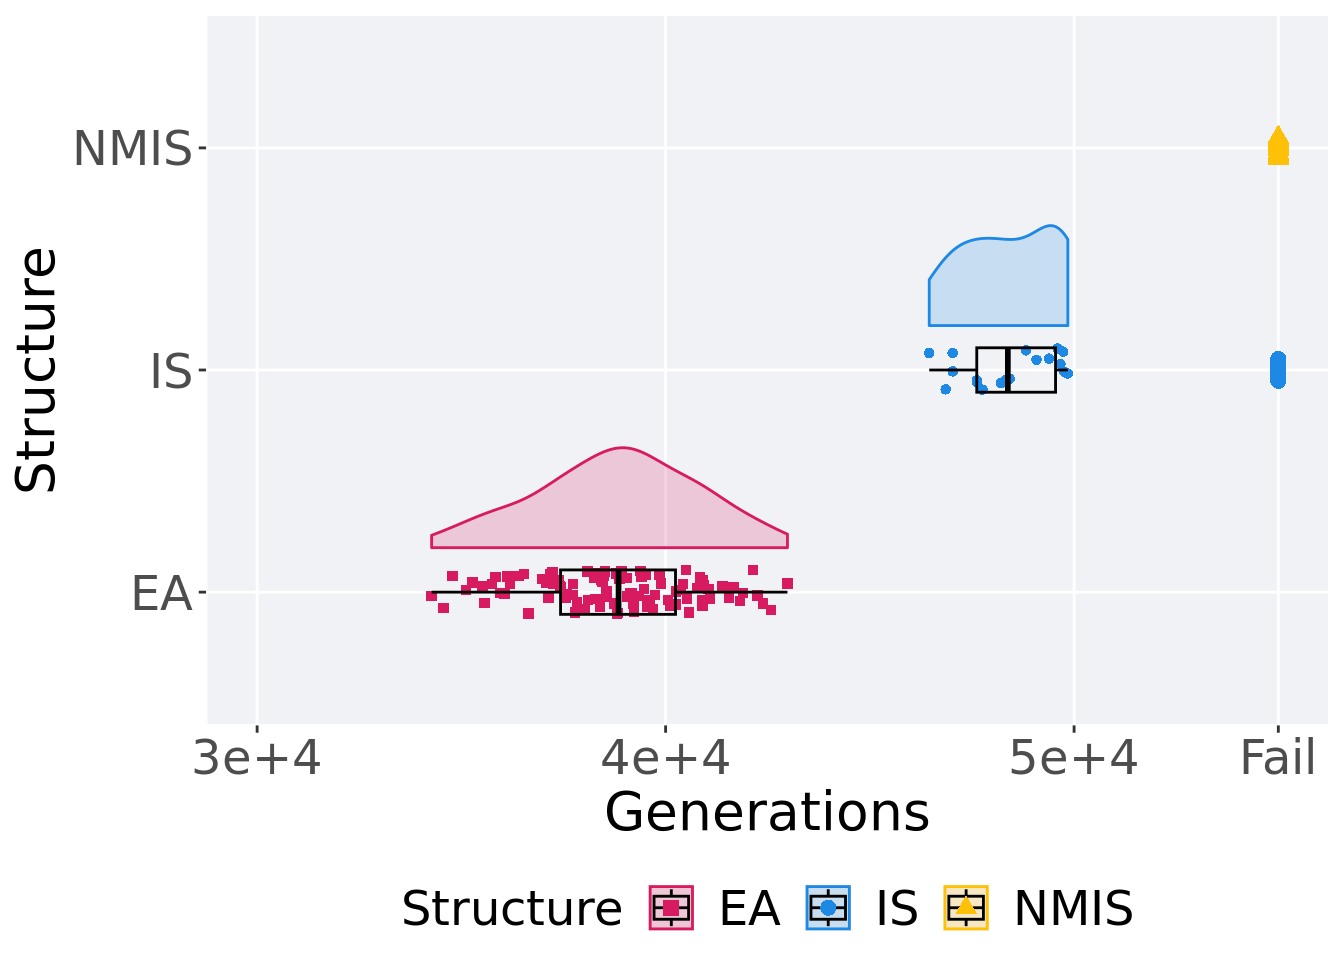
\includegraphics{demo_files/figure-latex/base-lex-ord-ssf-1.pdf}

\hypertarget{stats-7}{%
\subsubsection{Stats}\label{stats-7}}

Summary statistics for the first generation a satisfactory solution is found.

\begin{Shaded}
\begin{Highlighting}[]
\NormalTok{ssf =}\StringTok{ }\KeywordTok{filter}\NormalTok{(base_ssf, Diagnostic }\OperatorTok{==}\StringTok{ 'ORDERED_EXPLOITATION'} \OperatorTok{&}\StringTok{ `}\DataTypeTok{Selection}\CharTok{\textbackslash{}n}\DataTypeTok{Scheme}\StringTok{`} \OperatorTok{==}\StringTok{ 'LEXICASE'} \OperatorTok{&}\StringTok{ }\NormalTok{Generations }\OperatorTok{<}\StringTok{ }\DecValTok{60000}\NormalTok{)}
\NormalTok{ssf }\OperatorTok
\StringTok{  }\KeywordTok{group_by}\NormalTok{(Structure) }\OperatorTok
\StringTok{  }\NormalTok{dplyr}\OperatorTok{::}\KeywordTok{summarise}\NormalTok{(}
    \DataTypeTok{count =} \KeywordTok{n}\NormalTok{(),}
    \DataTypeTok{na_cnt =} \KeywordTok{sum}\NormalTok{(}\KeywordTok{is.na}\NormalTok{(Generations)),}
    \DataTypeTok{min =} \KeywordTok{min}\NormalTok{(Generations, }\DataTypeTok{na.rm =} \OtherTok{TRUE}\NormalTok{),}
    \DataTypeTok{median =} \KeywordTok{median}\NormalTok{(Generations, }\DataTypeTok{na.rm =} \OtherTok{TRUE}\NormalTok{),}
    \DataTypeTok{mean =} \KeywordTok{mean}\NormalTok{(Generations, }\DataTypeTok{na.rm =} \OtherTok{TRUE}\NormalTok{),}
    \DataTypeTok{max =} \KeywordTok{max}\NormalTok{(Generations, }\DataTypeTok{na.rm =} \OtherTok{TRUE}\NormalTok{),}
    \DataTypeTok{IQR =} \KeywordTok{IQR}\NormalTok{(Generations, }\DataTypeTok{na.rm =} \OtherTok{TRUE}\NormalTok{)}
\NormalTok{  )}
\end{Highlighting}
\end{Shaded}

\begin{verbatim}
## # A tibble: 2 x 8
##   Structure count na_cnt   min median   mean   max   IQR
##   <fct>     <int>  <int> <int>  <dbl>  <dbl> <int> <dbl>
## 1 EA          100      0 34272 38848  38795. 42983  2814
## 2 IS           18      0 46454 48378. 48402. 49847  1929
\end{verbatim}

Kruskal--Wallis test provides evidence of difference among selection schemes.

\begin{Shaded}
\begin{Highlighting}[]
\KeywordTok{kruskal.test}\NormalTok{(Generations }\OperatorTok{~}\StringTok{ }\NormalTok{Structure, }\DataTypeTok{data =}\NormalTok{ ssf)}
\end{Highlighting}
\end{Shaded}

\begin{verbatim}
## 
##  Kruskal-Wallis rank sum test
## 
## data:  Generations by Structure
## Kruskal-Wallis chi-squared = 45.378, df = 1, p-value = 1.624e-11
\end{verbatim}

Results for post-hoc Wilcoxon rank-sum test with a Bonferroni correction.

\begin{Shaded}
\begin{Highlighting}[]
\KeywordTok{pairwise.wilcox.test}\NormalTok{(}\DataTypeTok{x =}\NormalTok{ ssf}\OperatorTok{$}\NormalTok{Generations, }\DataTypeTok{g =}\NormalTok{ ssf}\OperatorTok{$}\NormalTok{Structure, }\DataTypeTok{p.adjust.method =} \StringTok{"bonferroni"}\NormalTok{,}
                     \DataTypeTok{paired =} \OtherTok{FALSE}\NormalTok{, }\DataTypeTok{conf.int =} \OtherTok{FALSE}\NormalTok{, }\DataTypeTok{alternative =} \StringTok{'g'}\NormalTok{)}
\end{Highlighting}
\end{Shaded}

\begin{verbatim}
## 
##  Pairwise comparisons using Wilcoxon rank sum test with continuity correction 
## 
## data:  ssf$Generations and ssf$Structure 
## 
##    EA     
## IS 8.3e-12
## 
## P value adjustment method: bonferroni
\end{verbatim}

\hypertarget{contradictory-objectives-results}{%
\chapter{Contradictory objectives results}\label{contradictory-objectives-results}}

Here we present the results for the \textbf{satisfactory trait corverage} and \textbf{activation gene coverage} generated by each selection scheme replicate on the contradictory objectives diagnostic with our base configurations.
Note both of these values are gathered at the population-level.
Activation gene coverage refers to the count of unique activation genes in a given population; this gives us a range of integers between 0 and 100.
Satisfactory trait coverage refers to the count of unique satisfied traits in a given population; this gives us a range of integers between 0 and 100.
For our base configuration, we execute migrations every 500 generations and there are 4 islands in a ring topology.
When migrations occur, two individuals are swapped (same position on each island) and guarantee that no solution can return to its original island.

\hypertarget{analysis-dependencies-2}{%
\section{Analysis dependencies}\label{analysis-dependencies-2}}

\begin{Shaded}
\begin{Highlighting}[]
\KeywordTok{library}\NormalTok{(ggplot2)}
\KeywordTok{library}\NormalTok{(cowplot)}
\KeywordTok{library}\NormalTok{(dplyr)}
\KeywordTok{library}\NormalTok{(PupillometryR)}
\end{Highlighting}
\end{Shaded}

\hypertarget{truncation-selection-2}{%
\section{Truncation selection}\label{truncation-selection-2}}

Here we analyze how the different population structures affect truncation selection (size 8) on the contradictory objectives diagnostic.

\hypertarget{satisfactory-trait-coverage}{%
\subsection{Satisfactory trait coverage}\label{satisfactory-trait-coverage}}

Satisfactory trait coverage analysis.

\hypertarget{coverage-over-time}{%
\subsubsection{Coverage over time}\label{coverage-over-time}}

Satisfactory trait coverage over time.

\begin{Shaded}
\begin{Highlighting}[]
\NormalTok{lines =}\StringTok{ }\KeywordTok{filter}\NormalTok{(base_over_time, Diagnostic }\OperatorTok{==}\StringTok{ 'CONTRADICTORY_OBJECTIVES'} \OperatorTok{&}\StringTok{ `}\DataTypeTok{Selection}\CharTok{\textbackslash{}n}\DataTypeTok{Scheme}\StringTok{`} \OperatorTok{==}\StringTok{ 'TRUNCATION'}\NormalTok{) }\OperatorTok
\StringTok{  }\KeywordTok{group_by}\NormalTok{(Structure, Generations) }\OperatorTok
\StringTok{  }\NormalTok{dplyr}\OperatorTok{::}\KeywordTok{summarise}\NormalTok{(}
    \DataTypeTok{min =} \KeywordTok{min}\NormalTok{(pop_sat_cov),}
    \DataTypeTok{mean =} \KeywordTok{mean}\NormalTok{(pop_sat_cov),}
    \DataTypeTok{max =} \KeywordTok{max}\NormalTok{(pop_sat_cov)}
\NormalTok{  )}
\end{Highlighting}
\end{Shaded}

\begin{verbatim}
## `summarise()` has grouped output by 'Structure'. You can override using the
## `.groups` argument.
\end{verbatim}

\begin{Shaded}
\begin{Highlighting}[]
\KeywordTok{ggplot}\NormalTok{(lines, }\KeywordTok{aes}\NormalTok{(}\DataTypeTok{x=}\NormalTok{Generations, }\DataTypeTok{y=}\NormalTok{mean, }\DataTypeTok{group =}\NormalTok{ Structure, }\DataTypeTok{fill =}\NormalTok{ Structure, }\DataTypeTok{color =}\NormalTok{ Structure, }\DataTypeTok{shape =}\NormalTok{ Structure)) }\OperatorTok{+}
\StringTok{  }\KeywordTok{geom_ribbon}\NormalTok{(}\KeywordTok{aes}\NormalTok{(}\DataTypeTok{ymin =}\NormalTok{ min, }\DataTypeTok{ymax =}\NormalTok{ max), }\DataTypeTok{alpha =} \FloatTok{0.1}\NormalTok{) }\OperatorTok{+}
\StringTok{  }\KeywordTok{geom_line}\NormalTok{(}\DataTypeTok{size =} \FloatTok{0.5}\NormalTok{) }\OperatorTok{+}
\StringTok{  }\KeywordTok{geom_point}\NormalTok{(}\DataTypeTok{data =} \KeywordTok{filter}\NormalTok{(lines, Generations }\OperatorTok\StringTok{ }\DecValTok{2000} \OperatorTok{==}\StringTok{ }\DecValTok{0}\NormalTok{), }\DataTypeTok{size =} \FloatTok{1.5}\NormalTok{, }\DataTypeTok{stroke =} \FloatTok{2.0}\NormalTok{, }\DataTypeTok{alpha =} \FloatTok{1.0}\NormalTok{) }\OperatorTok{+}
\StringTok{  }\KeywordTok{scale_y_continuous}\NormalTok{(}
    \DataTypeTok{name=}\StringTok{"Coverage"}
\NormalTok{  ) }\OperatorTok{+}
\StringTok{  }\KeywordTok{scale_x_continuous}\NormalTok{(}
    \DataTypeTok{name=}\StringTok{"Generations"}\NormalTok{,}
    \DataTypeTok{limits=}\KeywordTok{c}\NormalTok{(}\DecValTok{0}\NormalTok{, }\DecValTok{50000}\NormalTok{),}
    \DataTypeTok{breaks=}\KeywordTok{c}\NormalTok{(}\DecValTok{0}\NormalTok{, }\DecValTok{10000}\NormalTok{, }\DecValTok{20000}\NormalTok{, }\DecValTok{30000}\NormalTok{, }\DecValTok{40000}\NormalTok{, }\DecValTok{50000}\NormalTok{),}
    \DataTypeTok{labels=}\KeywordTok{c}\NormalTok{(}\StringTok{"0e+4"}\NormalTok{, }\StringTok{"1e+4"}\NormalTok{, }\StringTok{"2e+4"}\NormalTok{, }\StringTok{"3e+4"}\NormalTok{, }\StringTok{"4e+4"}\NormalTok{, }\StringTok{"5e+4"}\NormalTok{)}

\NormalTok{  ) }\OperatorTok{+}
\StringTok{  }\KeywordTok{scale_shape_manual}\NormalTok{(}\DataTypeTok{values=}\NormalTok{SHAPE)}\OperatorTok{+}
\StringTok{  }\KeywordTok{scale_colour_manual}\NormalTok{(}\DataTypeTok{values =}\NormalTok{ cb_palette) }\OperatorTok{+}
\StringTok{  }\KeywordTok{scale_fill_manual}\NormalTok{(}\DataTypeTok{values =}\NormalTok{ cb_palette) }\OperatorTok{+}
\StringTok{  }\KeywordTok{ggtitle}\NormalTok{(}\StringTok{'Satisfactory trait coverage over time'}\NormalTok{)}\OperatorTok{+}
\StringTok{  }\NormalTok{p_theme}
\end{Highlighting}
\end{Shaded}

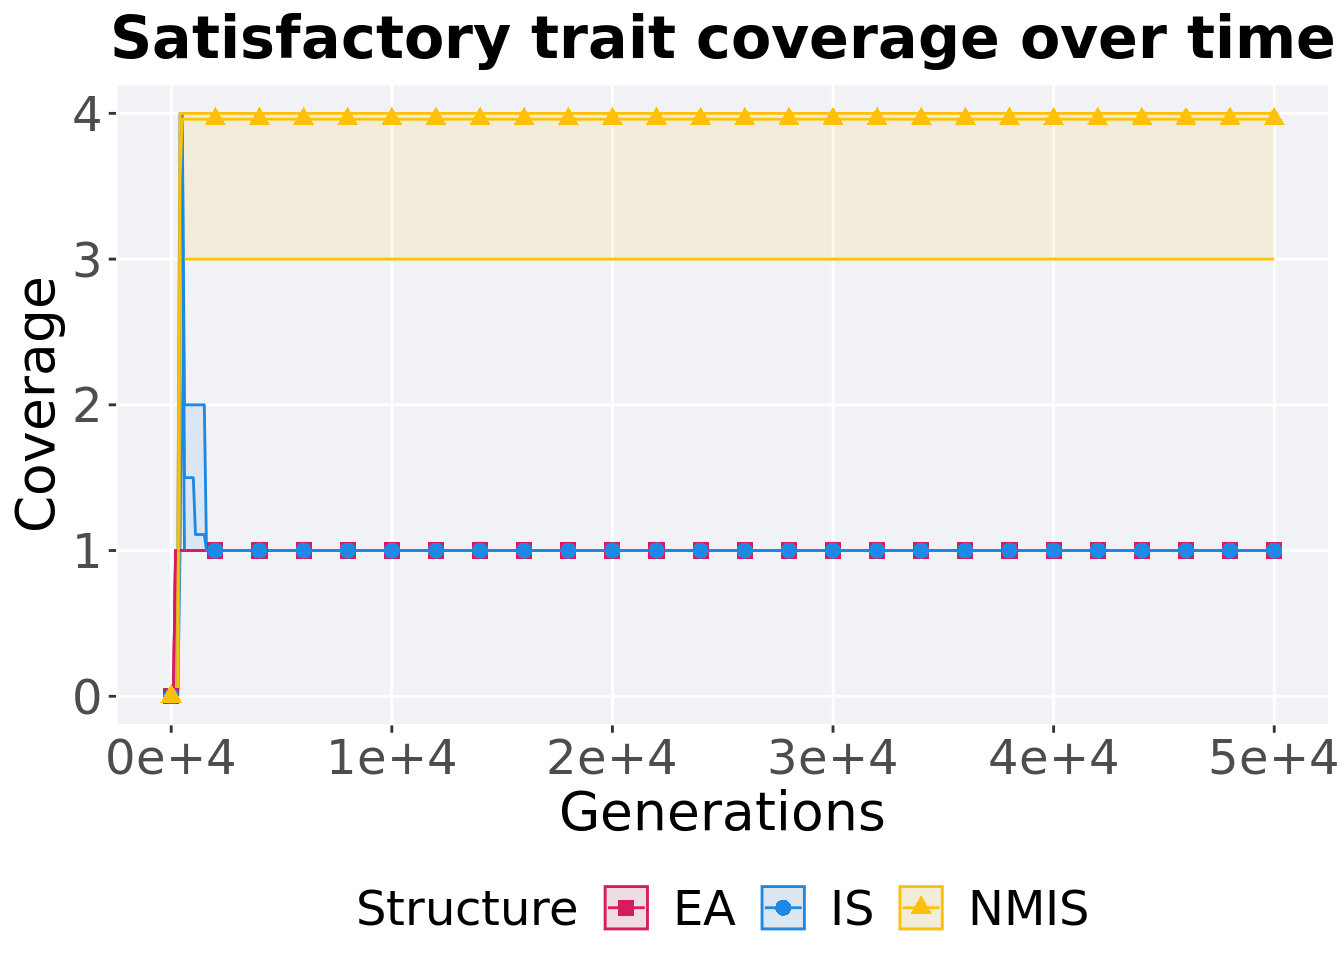
\includegraphics{demo_files/figure-latex/con-sat-tru-ot-1.pdf}

\hypertarget{best-coverage-throughout}{%
\subsubsection{Best coverage throughout}\label{best-coverage-throughout}}

Best satisfactory trait coverage throughout 50,000 generations.

\begin{Shaded}
\begin{Highlighting}[]
\CommentTok{### best satisfactory trait coverage throughout}
\KeywordTok{filter}\NormalTok{(base_best, Diagnostic }\OperatorTok{==}\StringTok{ 'CONTRADICTORY_OBJECTIVES'} \OperatorTok{&}\StringTok{ `}\DataTypeTok{Selection}\CharTok{\textbackslash{}n}\DataTypeTok{Scheme}\StringTok{`} \OperatorTok{==}\StringTok{ 'TRUNCATION'} \OperatorTok{&}\StringTok{ }\NormalTok{VAR }\OperatorTok{==}\StringTok{ 'pop_sat_cov'}\NormalTok{) }\OperatorTok
\StringTok{  }\KeywordTok{ggplot}\NormalTok{(., }\KeywordTok{aes}\NormalTok{(}\DataTypeTok{x =}\NormalTok{ Structure, }\DataTypeTok{y =}\NormalTok{ VAL, }\DataTypeTok{color =}\NormalTok{ Structure, }\DataTypeTok{fill =}\NormalTok{ Structure, }\DataTypeTok{shape =}\NormalTok{ Structure)) }\OperatorTok{+}
\StringTok{  }\KeywordTok{geom_flat_violin}\NormalTok{(}\DataTypeTok{position =} \KeywordTok{position_nudge}\NormalTok{(}\DataTypeTok{x =} \FloatTok{.2}\NormalTok{, }\DataTypeTok{y =} \DecValTok{0}\NormalTok{), }\DataTypeTok{scale =} \StringTok{'width'}\NormalTok{, }\DataTypeTok{alpha =} \FloatTok{0.2}\NormalTok{) }\OperatorTok{+}
\StringTok{  }\KeywordTok{geom_point}\NormalTok{(}\DataTypeTok{position =} \KeywordTok{position_jitter}\NormalTok{(}\DataTypeTok{height =} \FloatTok{.05}\NormalTok{, }\DataTypeTok{width =} \FloatTok{.05}\NormalTok{), }\DataTypeTok{size =} \FloatTok{1.5}\NormalTok{, }\DataTypeTok{alpha =} \FloatTok{1.0}\NormalTok{) }\OperatorTok{+}
\StringTok{  }\KeywordTok{geom_boxplot}\NormalTok{(}\DataTypeTok{color =} \StringTok{'black'}\NormalTok{, }\DataTypeTok{width =} \FloatTok{.2}\NormalTok{, }\DataTypeTok{outlier.shape =} \OtherTok{NA}\NormalTok{, }\DataTypeTok{alpha =} \FloatTok{0.0}\NormalTok{) }\OperatorTok{+}
\StringTok{  }\KeywordTok{scale_y_continuous}\NormalTok{(}
    \DataTypeTok{name=}\StringTok{"coverage"}
\NormalTok{  ) }\OperatorTok{+}
\StringTok{  }\KeywordTok{scale_x_discrete}\NormalTok{(}
    \DataTypeTok{name=}\StringTok{"Structure"}
\NormalTok{  )}\OperatorTok{+}
\StringTok{  }\KeywordTok{scale_shape_manual}\NormalTok{(}\DataTypeTok{values=}\NormalTok{SHAPE)}\OperatorTok{+}
\StringTok{  }\KeywordTok{scale_colour_manual}\NormalTok{(}\DataTypeTok{values =}\NormalTok{ cb_palette, ) }\OperatorTok{+}
\StringTok{  }\KeywordTok{scale_fill_manual}\NormalTok{(}\DataTypeTok{values =}\NormalTok{ cb_palette) }\OperatorTok{+}
\StringTok{  }\KeywordTok{ggtitle}\NormalTok{(}\StringTok{'Best satisfactory trait coverage'}\NormalTok{)}\OperatorTok{+}
\StringTok{  }\NormalTok{p_theme }\OperatorTok{+}\StringTok{ }\KeywordTok{coord_flip}\NormalTok{()}
\end{Highlighting}
\end{Shaded}

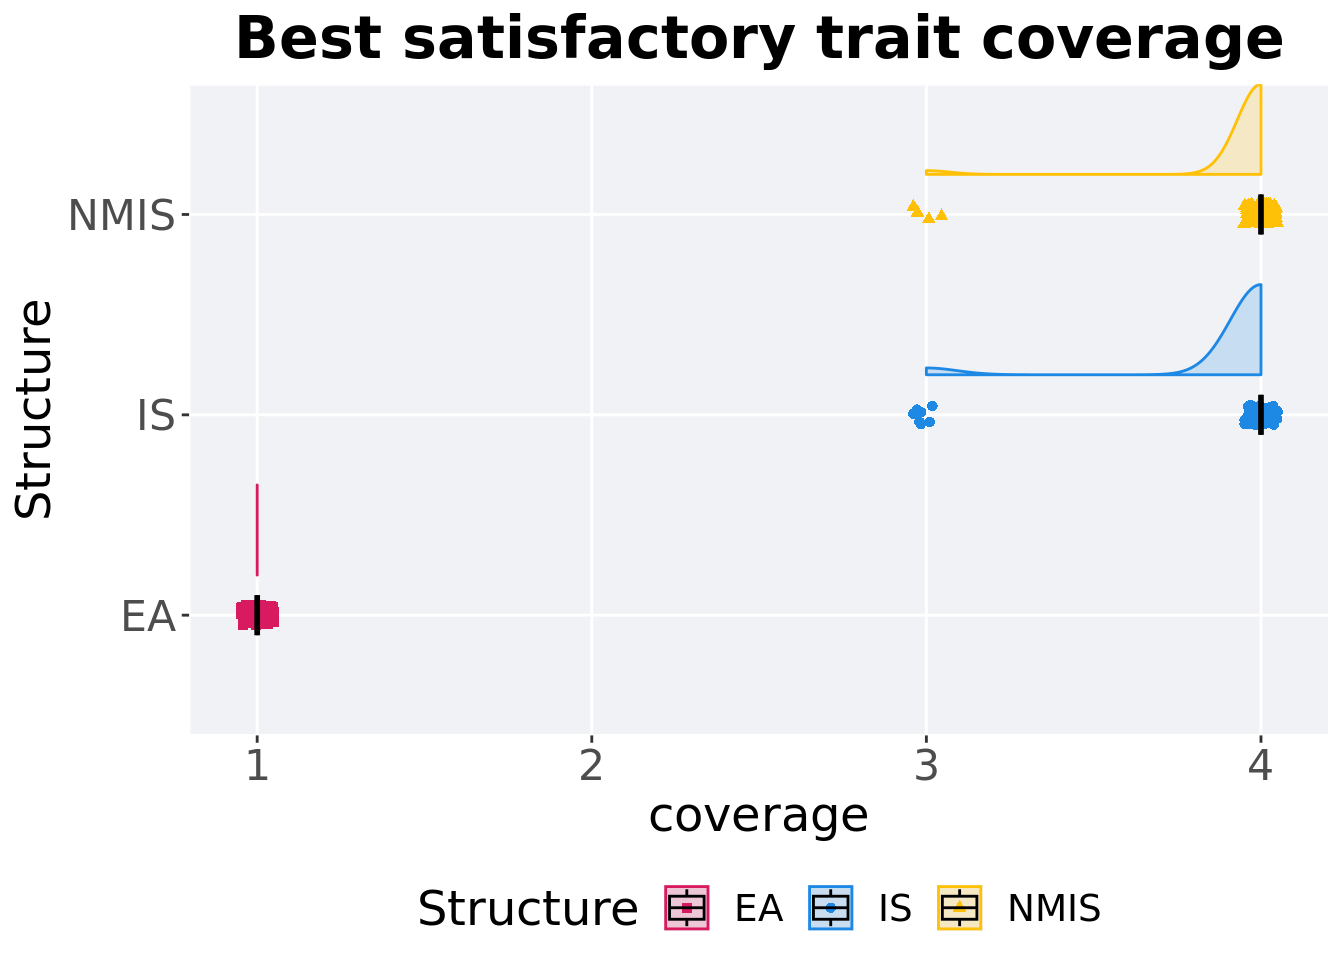
\includegraphics{demo_files/figure-latex/con-sat-tru-bst-1.pdf}

\hypertarget{stats-8}{%
\paragraph{Stats}\label{stats-8}}

Summary statistics for the best satisfactory trait coverage.

\begin{Shaded}
\begin{Highlighting}[]
\CommentTok{### best}
\NormalTok{coverage =}\StringTok{ }\KeywordTok{filter}\NormalTok{(base_best, Diagnostic }\OperatorTok{==}\StringTok{ 'CONTRADICTORY_OBJECTIVES'} \OperatorTok{&}\StringTok{ `}\DataTypeTok{Selection}\CharTok{\textbackslash{}n}\DataTypeTok{Scheme}\StringTok{`} \OperatorTok{==}\StringTok{ 'TRUNCATION'} \OperatorTok{&}\StringTok{ }\NormalTok{VAR }\OperatorTok{==}\StringTok{ 'pop_sat_cov'}\NormalTok{)}
\NormalTok{coverage }\OperatorTok
\StringTok{  }\KeywordTok{group_by}\NormalTok{(Structure) }\OperatorTok
\StringTok{  }\NormalTok{dplyr}\OperatorTok{::}\KeywordTok{summarise}\NormalTok{(}
    \DataTypeTok{count =} \KeywordTok{n}\NormalTok{(),}
    \DataTypeTok{na_cnt =} \KeywordTok{sum}\NormalTok{(}\KeywordTok{is.na}\NormalTok{(VAL)),}
    \DataTypeTok{min =} \KeywordTok{min}\NormalTok{(VAL, }\DataTypeTok{na.rm =} \OtherTok{TRUE}\NormalTok{),}
    \DataTypeTok{median =} \KeywordTok{median}\NormalTok{(VAL, }\DataTypeTok{na.rm =} \OtherTok{TRUE}\NormalTok{),}
    \DataTypeTok{mean =} \KeywordTok{mean}\NormalTok{(VAL, }\DataTypeTok{na.rm =} \OtherTok{TRUE}\NormalTok{),}
    \DataTypeTok{max =} \KeywordTok{max}\NormalTok{(VAL, }\DataTypeTok{na.rm =} \OtherTok{TRUE}\NormalTok{),}
    \DataTypeTok{IQR =} \KeywordTok{IQR}\NormalTok{(VAL, }\DataTypeTok{na.rm =} \OtherTok{TRUE}\NormalTok{)}
\NormalTok{  )}
\end{Highlighting}
\end{Shaded}

\begin{verbatim}
## # A tibble: 3 x 8
##   Structure count na_cnt   min median  mean   max   IQR
##   <fct>     <int>  <int> <dbl>  <dbl> <dbl> <dbl> <dbl>
## 1 EA          100      0     1      1  1        1     0
## 2 IS          100      0     3      4  3.93     4     0
## 3 NMIS        100      0     3      4  3.96     4     0
\end{verbatim}

Kruskal--Wallis test provides evidence of difference among satisfactory trait coverage.

\begin{Shaded}
\begin{Highlighting}[]
\KeywordTok{kruskal.test}\NormalTok{(VAL }\OperatorTok{~}\StringTok{ }\NormalTok{Structure, }\DataTypeTok{data =}\NormalTok{ coverage)}
\end{Highlighting}
\end{Shaded}

\begin{verbatim}
## 
##  Kruskal-Wallis rank sum test
## 
## data:  VAL by Structure
## Kruskal-Wallis chi-squared = 279.71, df = 2, p-value < 2.2e-16
\end{verbatim}

Results for post-hoc Wilcoxon rank-sum test with a Bonferroni correction on satisfactory trait coverage.

\begin{Shaded}
\begin{Highlighting}[]
\KeywordTok{pairwise.wilcox.test}\NormalTok{(}\DataTypeTok{x =}\NormalTok{ coverage}\OperatorTok{$}\NormalTok{VAL, }\DataTypeTok{g =}\NormalTok{ coverage}\OperatorTok{$}\NormalTok{Structure, }\DataTypeTok{p.adjust.method =} \StringTok{"bonferroni"}\NormalTok{,}
                     \DataTypeTok{paired =} \OtherTok{FALSE}\NormalTok{, }\DataTypeTok{conf.int =} \OtherTok{FALSE}\NormalTok{, }\DataTypeTok{alternative =} \StringTok{'g'}\NormalTok{)}
\end{Highlighting}
\end{Shaded}

\begin{verbatim}
## 
##  Pairwise comparisons using Wilcoxon rank sum test with continuity correction 
## 
## data:  coverage$VAL and coverage$Structure 
## 
##      EA     IS  
## IS   <2e-16 -   
## NMIS <2e-16 0.53
## 
## P value adjustment method: bonferroni
\end{verbatim}

\hypertarget{end-of-50000-generations}{%
\subsubsection{End of 50,000 generations}\label{end-of-50000-generations}}

Satisfactory trait coverage in the population at the end of 50,000 generations.

\begin{Shaded}
\begin{Highlighting}[]
\CommentTok{### end of run}
\KeywordTok{filter}\NormalTok{(base_over_time, Diagnostic }\OperatorTok{==}\StringTok{ 'CONTRADICTORY_OBJECTIVES'} \OperatorTok{&}\StringTok{ `}\DataTypeTok{Selection}\CharTok{\textbackslash{}n}\DataTypeTok{Scheme}\StringTok{`} \OperatorTok{==}\StringTok{ 'TRUNCATION'} \OperatorTok{&}\StringTok{ }\NormalTok{Generations }\OperatorTok{==}\StringTok{ }\DecValTok{50000}\NormalTok{) }\OperatorTok
\StringTok{  }\KeywordTok{ggplot}\NormalTok{(., }\KeywordTok{aes}\NormalTok{(}\DataTypeTok{x =}\NormalTok{ Structure, }\DataTypeTok{y =}\NormalTok{ pop_sat_cov, }\DataTypeTok{color =}\NormalTok{ Structure, }\DataTypeTok{fill =}\NormalTok{ Structure, }\DataTypeTok{shape =}\NormalTok{ Structure)) }\OperatorTok{+}
\StringTok{  }\KeywordTok{geom_flat_violin}\NormalTok{(}\DataTypeTok{position =} \KeywordTok{position_nudge}\NormalTok{(}\DataTypeTok{x =} \FloatTok{.2}\NormalTok{, }\DataTypeTok{y =} \DecValTok{0}\NormalTok{), }\DataTypeTok{scale =} \StringTok{'width'}\NormalTok{, }\DataTypeTok{alpha =} \FloatTok{0.3}\NormalTok{) }\OperatorTok{+}
\StringTok{  }\KeywordTok{geom_point}\NormalTok{(}\DataTypeTok{position =} \KeywordTok{position_jitter}\NormalTok{(}\DataTypeTok{height =} \FloatTok{.05}\NormalTok{, }\DataTypeTok{width =} \FloatTok{.05}\NormalTok{), }\DataTypeTok{size =} \FloatTok{1.5}\NormalTok{, }\DataTypeTok{alpha =} \FloatTok{0.5}\NormalTok{) }\OperatorTok{+}
\StringTok{  }\KeywordTok{geom_boxplot}\NormalTok{(}\DataTypeTok{color =} \StringTok{'black'}\NormalTok{, }\DataTypeTok{width =} \FloatTok{.2}\NormalTok{, }\DataTypeTok{outlier.shape =} \OtherTok{NA}\NormalTok{, }\DataTypeTok{alpha =} \FloatTok{0.0}\NormalTok{) }\OperatorTok{+}
\StringTok{  }\KeywordTok{scale_shape_manual}\NormalTok{(}\DataTypeTok{values=}\NormalTok{SHAPE)}\OperatorTok{+}
\StringTok{  }\KeywordTok{scale_y_continuous}\NormalTok{(}
    \DataTypeTok{name=}\StringTok{"Coverage"}
\NormalTok{  ) }\OperatorTok{+}
\StringTok{  }\KeywordTok{scale_x_discrete}\NormalTok{(}
    \DataTypeTok{name=}\StringTok{"Structure"}
\NormalTok{  ) }\OperatorTok{+}
\StringTok{  }\KeywordTok{scale_colour_manual}\NormalTok{(}\DataTypeTok{values =}\NormalTok{ cb_palette) }\OperatorTok{+}
\StringTok{  }\KeywordTok{scale_fill_manual}\NormalTok{(}\DataTypeTok{values =}\NormalTok{ cb_palette) }\OperatorTok{+}
\StringTok{  }\KeywordTok{ggtitle}\NormalTok{(}\StringTok{'Final satisfactory trait coverage'}\NormalTok{)}\OperatorTok{+}
\StringTok{  }\NormalTok{p_theme }\OperatorTok{+}\StringTok{ }\KeywordTok{coord_flip}\NormalTok{()}
\end{Highlighting}
\end{Shaded}

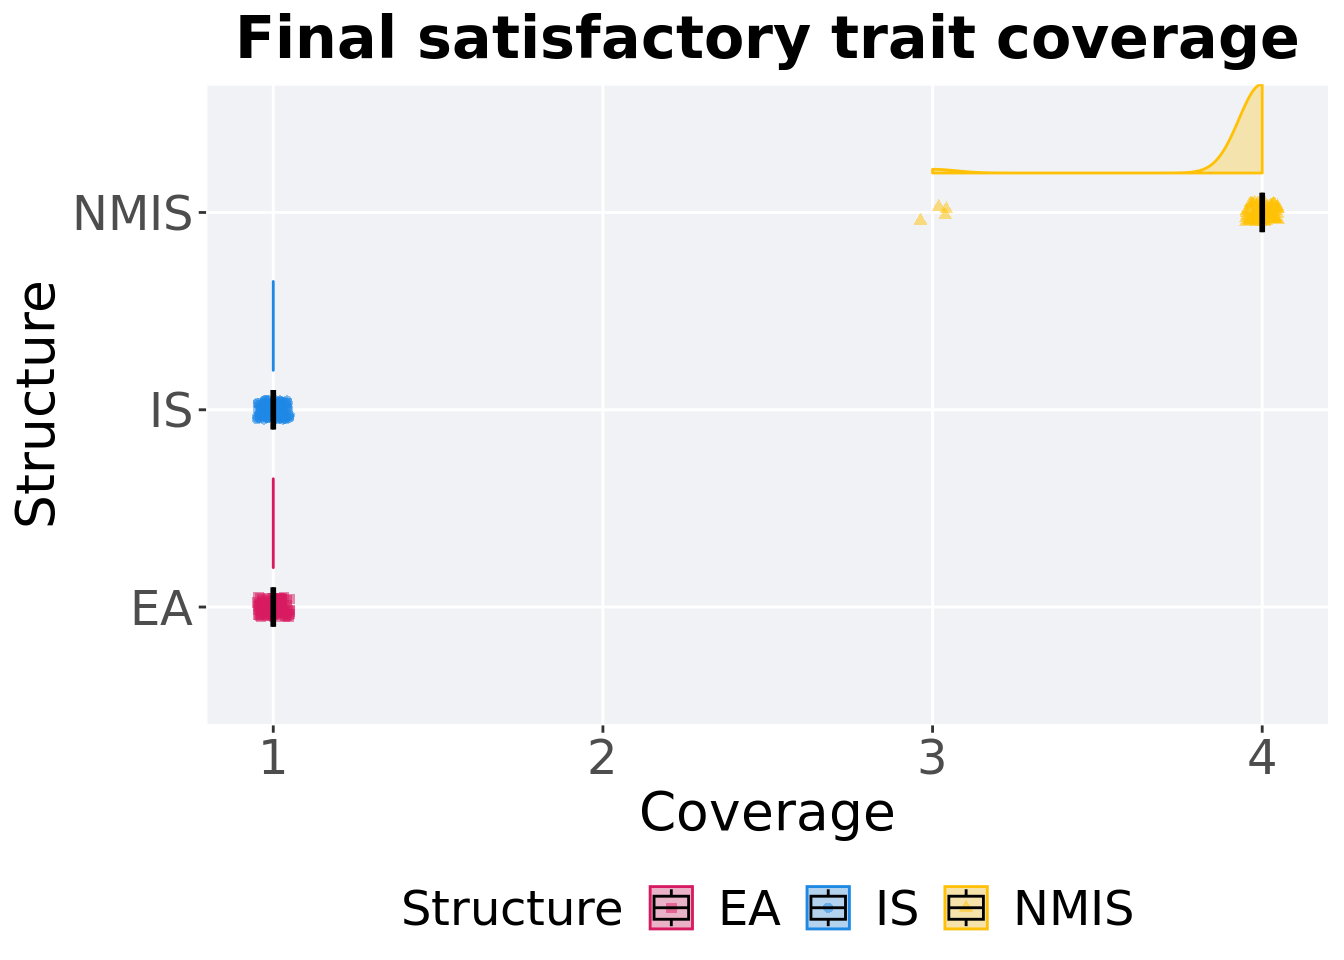
\includegraphics{demo_files/figure-latex/con-sat-tru-end-1.pdf}

\hypertarget{stats-9}{%
\paragraph{Stats}\label{stats-9}}

Summary statistics for satisfactory trait coverage in the population at the end of 50,000 generations.

\begin{Shaded}
\begin{Highlighting}[]
\CommentTok{### end of run}
\NormalTok{coverage =}\StringTok{ }\KeywordTok{filter}\NormalTok{(base_over_time, Diagnostic }\OperatorTok{==}\StringTok{ 'CONTRADICTORY_OBJECTIVES'} \OperatorTok{&}\StringTok{ `}\DataTypeTok{Selection}\CharTok{\textbackslash{}n}\DataTypeTok{Scheme}\StringTok{`} \OperatorTok{==}\StringTok{ 'TRUNCATION'} \OperatorTok{&}\StringTok{ }\NormalTok{Generations }\OperatorTok{==}\StringTok{ }\DecValTok{50000}\NormalTok{)}
\NormalTok{coverage }\OperatorTok
\StringTok{  }\KeywordTok{group_by}\NormalTok{(Structure) }\OperatorTok
\StringTok{  }\NormalTok{dplyr}\OperatorTok{::}\KeywordTok{summarise}\NormalTok{(}
    \DataTypeTok{count =} \KeywordTok{n}\NormalTok{(),}
    \DataTypeTok{na_cnt =} \KeywordTok{sum}\NormalTok{(}\KeywordTok{is.na}\NormalTok{(pop_sat_cov)),}
    \DataTypeTok{min =} \KeywordTok{min}\NormalTok{(pop_sat_cov, }\DataTypeTok{na.rm =} \OtherTok{TRUE}\NormalTok{),}
    \DataTypeTok{median =} \KeywordTok{median}\NormalTok{(pop_sat_cov, }\DataTypeTok{na.rm =} \OtherTok{TRUE}\NormalTok{),}
    \DataTypeTok{mean =} \KeywordTok{mean}\NormalTok{(pop_sat_cov, }\DataTypeTok{na.rm =} \OtherTok{TRUE}\NormalTok{),}
    \DataTypeTok{max =} \KeywordTok{max}\NormalTok{(pop_sat_cov, }\DataTypeTok{na.rm =} \OtherTok{TRUE}\NormalTok{),}
    \DataTypeTok{IQR =} \KeywordTok{IQR}\NormalTok{(pop_sat_cov, }\DataTypeTok{na.rm =} \OtherTok{TRUE}\NormalTok{)}
\NormalTok{  )}
\end{Highlighting}
\end{Shaded}

\begin{verbatim}
## # A tibble: 3 x 8
##   Structure count na_cnt   min median  mean   max   IQR
##   <fct>     <int>  <int> <int>  <dbl> <dbl> <int> <dbl>
## 1 EA          100      0     1      1  1        1     0
## 2 IS          100      0     1      1  1        1     0
## 3 NMIS        100      0     3      4  3.96     4     0
\end{verbatim}

Kruskal--Wallis test provides evidence of difference among satisfactory trait coverage in the population at the end of 50,000 generations.

\begin{Shaded}
\begin{Highlighting}[]
\KeywordTok{kruskal.test}\NormalTok{(pop_sat_cov }\OperatorTok{~}\StringTok{ }\NormalTok{Structure, }\DataTypeTok{data =}\NormalTok{ coverage)}
\end{Highlighting}
\end{Shaded}

\begin{verbatim}
## 
##  Kruskal-Wallis rank sum test
## 
## data:  pop_sat_cov by Structure
## Kruskal-Wallis chi-squared = 297.1, df = 2, p-value < 2.2e-16
\end{verbatim}

Results for post-hoc Wilcoxon rank-sum test with a Bonferroni correction on satisfactory trait coverage in the population at the end of 50,000 generations.

\begin{Shaded}
\begin{Highlighting}[]
\KeywordTok{pairwise.wilcox.test}\NormalTok{(}\DataTypeTok{x =}\NormalTok{ coverage}\OperatorTok{$}\NormalTok{pop_sat_cov, }\DataTypeTok{g =}\NormalTok{ coverage}\OperatorTok{$}\NormalTok{Structure, }\DataTypeTok{p.adjust.method =} \StringTok{"bonferroni"}\NormalTok{,}
                     \DataTypeTok{paired =} \OtherTok{FALSE}\NormalTok{, }\DataTypeTok{conf.int =} \OtherTok{FALSE}\NormalTok{, }\DataTypeTok{alternative =} \StringTok{'g'}\NormalTok{)}
\end{Highlighting}
\end{Shaded}

\begin{verbatim}
## 
##  Pairwise comparisons using Wilcoxon rank sum test with continuity correction 
## 
## data:  coverage$pop_sat_cov and coverage$Structure 
## 
##      EA     IS    
## IS   1      -     
## NMIS <2e-16 <2e-16
## 
## P value adjustment method: bonferroni
\end{verbatim}

\hypertarget{activation-gene-coverage}{%
\subsection{Activation gene coverage}\label{activation-gene-coverage}}

Activation gene coverage analysis.

\hypertarget{coverage-over-time-1}{%
\subsubsection{Coverage over time}\label{coverage-over-time-1}}

Activation gene coverage over time.

\begin{Shaded}
\begin{Highlighting}[]
\CommentTok{# data for lines and shading on plots}
\NormalTok{lines =}\StringTok{ }\KeywordTok{filter}\NormalTok{(base_over_time, Diagnostic }\OperatorTok{==}\StringTok{ 'CONTRADICTORY_OBJECTIVES'} \OperatorTok{&}\StringTok{ `}\DataTypeTok{Selection}\CharTok{\textbackslash{}n}\DataTypeTok{Scheme}\StringTok{`} \OperatorTok{==}\StringTok{ 'TRUNCATION'}\NormalTok{) }\OperatorTok
\StringTok{  }\KeywordTok{group_by}\NormalTok{(Structure, Generations) }\OperatorTok
\StringTok{  }\NormalTok{dplyr}\OperatorTok{::}\KeywordTok{summarise}\NormalTok{(}
    \DataTypeTok{min =} \KeywordTok{min}\NormalTok{(pop_act_cov),}
    \DataTypeTok{mean =} \KeywordTok{mean}\NormalTok{(pop_act_cov),}
    \DataTypeTok{max =} \KeywordTok{max}\NormalTok{(pop_act_cov)}
\NormalTok{  )}
\end{Highlighting}
\end{Shaded}

\begin{verbatim}
## `summarise()` has grouped output by 'Structure'. You can override using the
## `.groups` argument.
\end{verbatim}

\begin{Shaded}
\begin{Highlighting}[]
\KeywordTok{ggplot}\NormalTok{(lines, }\KeywordTok{aes}\NormalTok{(}\DataTypeTok{x=}\NormalTok{Generations, }\DataTypeTok{y=}\NormalTok{mean, }\DataTypeTok{group =}\NormalTok{ Structure, }\DataTypeTok{fill =}\NormalTok{ Structure, }\DataTypeTok{color =}\NormalTok{ Structure, }\DataTypeTok{shape =}\NormalTok{ Structure)) }\OperatorTok{+}
\StringTok{  }\KeywordTok{geom_ribbon}\NormalTok{(}\KeywordTok{aes}\NormalTok{(}\DataTypeTok{ymin =}\NormalTok{ min, }\DataTypeTok{ymax =}\NormalTok{ max), }\DataTypeTok{alpha =} \FloatTok{0.1}\NormalTok{) }\OperatorTok{+}
\StringTok{  }\KeywordTok{geom_line}\NormalTok{(}\DataTypeTok{size =} \FloatTok{0.5}\NormalTok{) }\OperatorTok{+}
\StringTok{  }\KeywordTok{geom_point}\NormalTok{(}\DataTypeTok{data =} \KeywordTok{filter}\NormalTok{(lines, Generations }\OperatorTok\StringTok{ }\DecValTok{2000} \OperatorTok{==}\StringTok{ }\DecValTok{0}\NormalTok{), }\DataTypeTok{size =} \FloatTok{1.5}\NormalTok{, }\DataTypeTok{stroke =} \FloatTok{2.0}\NormalTok{, }\DataTypeTok{alpha =} \FloatTok{1.0}\NormalTok{) }\OperatorTok{+}
\StringTok{  }\KeywordTok{scale_y_continuous}\NormalTok{(}
    \DataTypeTok{name=}\StringTok{"Coverage"}
\NormalTok{  ) }\OperatorTok{+}
\StringTok{  }\KeywordTok{scale_x_continuous}\NormalTok{(}
    \DataTypeTok{name=}\StringTok{"Generations"}\NormalTok{,}
    \DataTypeTok{limits=}\KeywordTok{c}\NormalTok{(}\DecValTok{0}\NormalTok{, }\DecValTok{50000}\NormalTok{),}
    \DataTypeTok{breaks=}\KeywordTok{c}\NormalTok{(}\DecValTok{0}\NormalTok{, }\DecValTok{10000}\NormalTok{, }\DecValTok{20000}\NormalTok{, }\DecValTok{30000}\NormalTok{, }\DecValTok{40000}\NormalTok{, }\DecValTok{50000}\NormalTok{),}
    \DataTypeTok{labels=}\KeywordTok{c}\NormalTok{(}\StringTok{"0e+4"}\NormalTok{, }\StringTok{"1e+4"}\NormalTok{, }\StringTok{"2e+4"}\NormalTok{, }\StringTok{"3e+4"}\NormalTok{, }\StringTok{"4e+4"}\NormalTok{, }\StringTok{"5e+4"}\NormalTok{)}

\NormalTok{  ) }\OperatorTok{+}
\StringTok{  }\KeywordTok{scale_shape_manual}\NormalTok{(}\DataTypeTok{values=}\NormalTok{SHAPE)}\OperatorTok{+}
\StringTok{  }\KeywordTok{scale_colour_manual}\NormalTok{(}\DataTypeTok{values =}\NormalTok{ cb_palette) }\OperatorTok{+}
\StringTok{  }\KeywordTok{scale_fill_manual}\NormalTok{(}\DataTypeTok{values =}\NormalTok{ cb_palette) }\OperatorTok{+}
\StringTok{  }\KeywordTok{ggtitle}\NormalTok{(}\StringTok{'Activation gene coverage over time'}\NormalTok{)}\OperatorTok{+}
\StringTok{  }\NormalTok{p_theme}
\end{Highlighting}
\end{Shaded}

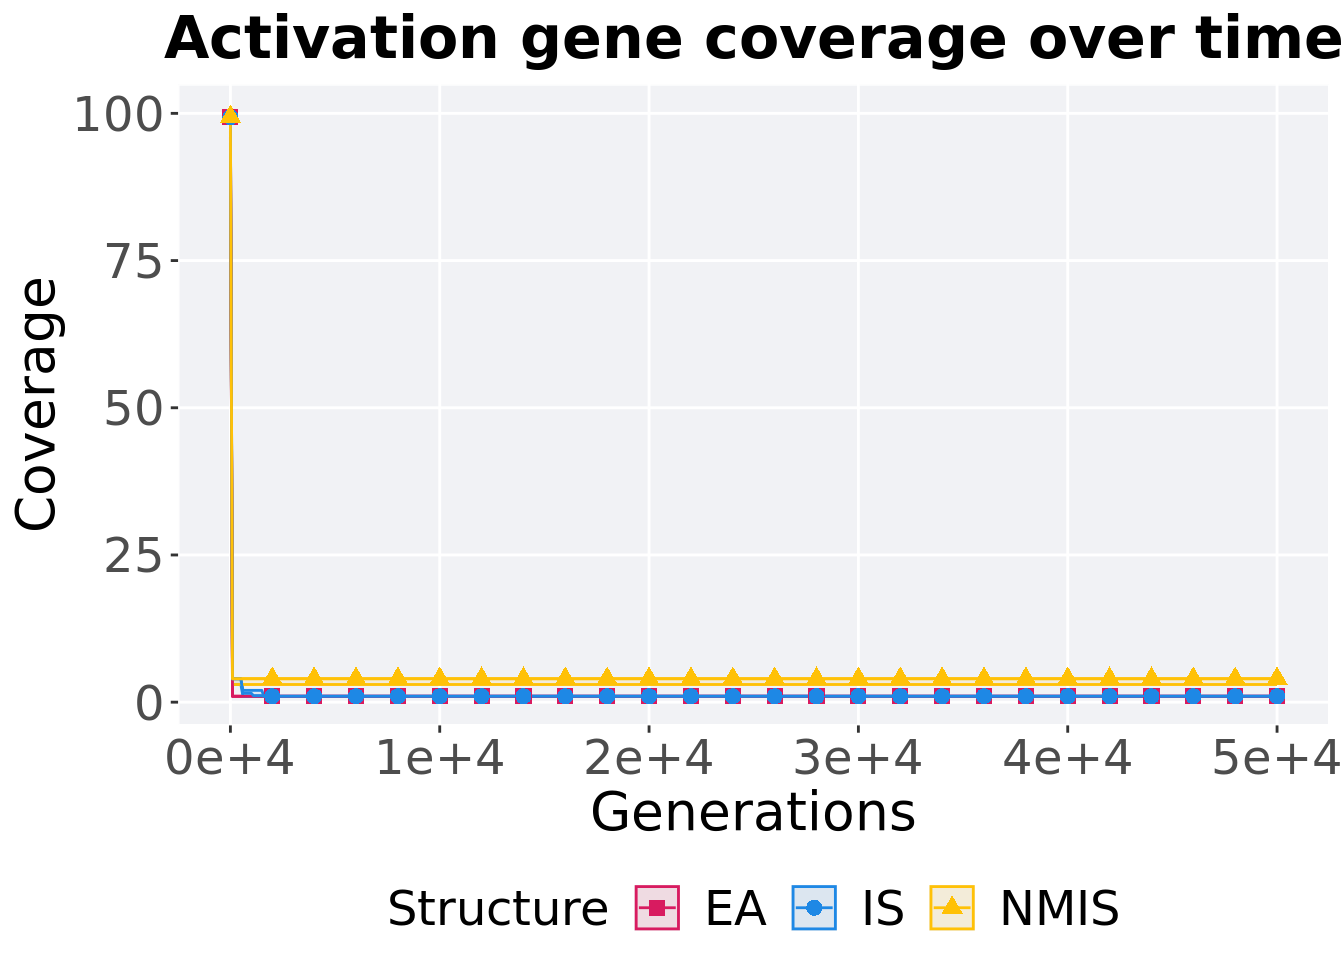
\includegraphics{demo_files/figure-latex/con-act-tru-ot-1.pdf}

\hypertarget{end-of-50000-generations-1}{%
\subsubsection{End of 50,000 generations}\label{end-of-50000-generations-1}}

Activation gene coverage in the population at the end of 50,000 generations.

\begin{Shaded}
\begin{Highlighting}[]
\CommentTok{### end of run}
\KeywordTok{filter}\NormalTok{(base_over_time, Diagnostic }\OperatorTok{==}\StringTok{ 'CONTRADICTORY_OBJECTIVES'} \OperatorTok{&}\StringTok{ `}\DataTypeTok{Selection}\CharTok{\textbackslash{}n}\DataTypeTok{Scheme}\StringTok{`} \OperatorTok{==}\StringTok{ 'TRUNCATION'} \OperatorTok{&}\StringTok{ }\NormalTok{Generations }\OperatorTok{==}\StringTok{ }\DecValTok{50000}\NormalTok{) }\OperatorTok
\StringTok{  }\KeywordTok{ggplot}\NormalTok{(., }\KeywordTok{aes}\NormalTok{(}\DataTypeTok{x =}\NormalTok{ Structure, }\DataTypeTok{y =}\NormalTok{ pop_act_cov, }\DataTypeTok{color =}\NormalTok{ Structure, }\DataTypeTok{fill =}\NormalTok{ Structure, }\DataTypeTok{shape =}\NormalTok{ Structure)) }\OperatorTok{+}
\StringTok{  }\KeywordTok{geom_flat_violin}\NormalTok{(}\DataTypeTok{position =} \KeywordTok{position_nudge}\NormalTok{(}\DataTypeTok{x =} \FloatTok{.2}\NormalTok{, }\DataTypeTok{y =} \DecValTok{0}\NormalTok{), }\DataTypeTok{scale =} \StringTok{'width'}\NormalTok{, }\DataTypeTok{alpha =} \FloatTok{0.3}\NormalTok{) }\OperatorTok{+}
\StringTok{  }\KeywordTok{geom_point}\NormalTok{(}\DataTypeTok{position =} \KeywordTok{position_jitter}\NormalTok{(}\DataTypeTok{height =} \FloatTok{.05}\NormalTok{, }\DataTypeTok{width =} \FloatTok{.05}\NormalTok{), }\DataTypeTok{size =} \FloatTok{1.5}\NormalTok{, }\DataTypeTok{alpha =} \FloatTok{0.5}\NormalTok{) }\OperatorTok{+}
\StringTok{  }\KeywordTok{geom_boxplot}\NormalTok{(}\DataTypeTok{color =} \StringTok{'black'}\NormalTok{, }\DataTypeTok{width =} \FloatTok{.2}\NormalTok{, }\DataTypeTok{outlier.shape =} \OtherTok{NA}\NormalTok{, }\DataTypeTok{alpha =} \FloatTok{0.0}\NormalTok{) }\OperatorTok{+}
\StringTok{  }\KeywordTok{scale_shape_manual}\NormalTok{(}\DataTypeTok{values=}\NormalTok{SHAPE)}\OperatorTok{+}
\StringTok{  }\KeywordTok{scale_y_continuous}\NormalTok{(}
    \DataTypeTok{name=}\StringTok{"Coverage"}
\NormalTok{  ) }\OperatorTok{+}
\StringTok{  }\KeywordTok{scale_x_discrete}\NormalTok{(}
    \DataTypeTok{name=}\StringTok{"Structure"}
\NormalTok{  ) }\OperatorTok{+}
\StringTok{  }\KeywordTok{scale_colour_manual}\NormalTok{(}\DataTypeTok{values =}\NormalTok{ cb_palette) }\OperatorTok{+}
\StringTok{  }\KeywordTok{scale_fill_manual}\NormalTok{(}\DataTypeTok{values =}\NormalTok{ cb_palette) }\OperatorTok{+}
\StringTok{  }\KeywordTok{ggtitle}\NormalTok{(}\StringTok{'Final activation gene coverage'}\NormalTok{)}\OperatorTok{+}
\StringTok{  }\NormalTok{p_theme }\OperatorTok{+}\StringTok{ }\KeywordTok{coord_flip}\NormalTok{()}
\end{Highlighting}
\end{Shaded}

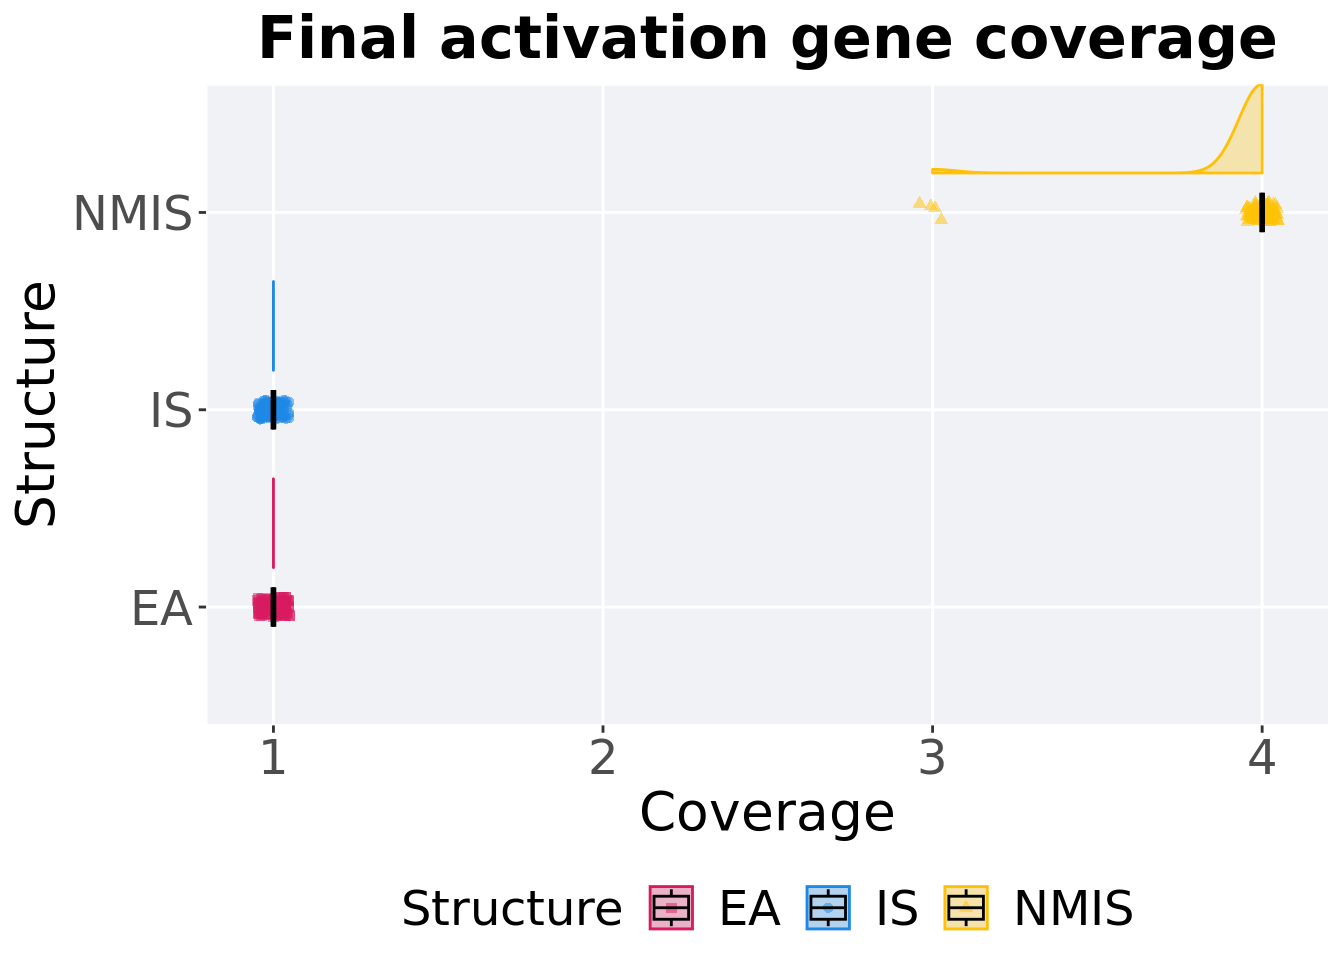
\includegraphics{demo_files/figure-latex/con-act-tru-end-1.pdf}

\hypertarget{stats-10}{%
\paragraph{Stats}\label{stats-10}}

Summary statistics for activation gene coverage.

\begin{Shaded}
\begin{Highlighting}[]
\NormalTok{coverage =}\StringTok{ }\KeywordTok{filter}\NormalTok{(base_over_time, Diagnostic }\OperatorTok{==}\StringTok{ 'CONTRADICTORY_OBJECTIVES'} \OperatorTok{&}\StringTok{ `}\DataTypeTok{Selection}\CharTok{\textbackslash{}n}\DataTypeTok{Scheme}\StringTok{`} \OperatorTok{==}\StringTok{ 'TRUNCATION'} \OperatorTok{&}\StringTok{ }\NormalTok{Generations }\OperatorTok{==}\StringTok{ }\DecValTok{50000}\NormalTok{)}
\NormalTok{coverage }\OperatorTok
\StringTok{  }\KeywordTok{group_by}\NormalTok{(Structure) }\OperatorTok
\StringTok{  }\NormalTok{dplyr}\OperatorTok{::}\KeywordTok{summarise}\NormalTok{(}
    \DataTypeTok{count =} \KeywordTok{n}\NormalTok{(),}
    \DataTypeTok{na_cnt =} \KeywordTok{sum}\NormalTok{(}\KeywordTok{is.na}\NormalTok{(pop_act_cov)),}
    \DataTypeTok{min =} \KeywordTok{min}\NormalTok{(pop_act_cov, }\DataTypeTok{na.rm =} \OtherTok{TRUE}\NormalTok{),}
    \DataTypeTok{median =} \KeywordTok{median}\NormalTok{(pop_act_cov, }\DataTypeTok{na.rm =} \OtherTok{TRUE}\NormalTok{),}
    \DataTypeTok{mean =} \KeywordTok{mean}\NormalTok{(pop_act_cov, }\DataTypeTok{na.rm =} \OtherTok{TRUE}\NormalTok{),}
    \DataTypeTok{max =} \KeywordTok{max}\NormalTok{(pop_act_cov, }\DataTypeTok{na.rm =} \OtherTok{TRUE}\NormalTok{),}
    \DataTypeTok{IQR =} \KeywordTok{IQR}\NormalTok{(pop_act_cov, }\DataTypeTok{na.rm =} \OtherTok{TRUE}\NormalTok{)}
\NormalTok{  )}
\end{Highlighting}
\end{Shaded}

\begin{verbatim}
## # A tibble: 3 x 8
##   Structure count na_cnt   min median  mean   max   IQR
##   <fct>     <int>  <int> <int>  <dbl> <dbl> <int> <dbl>
## 1 EA          100      0     1      1  1        1     0
## 2 IS          100      0     1      1  1        1     0
## 3 NMIS        100      0     3      4  3.96     4     0
\end{verbatim}

Kruskal--Wallis test provides evidence of difference among activation gene coverage.

\begin{Shaded}
\begin{Highlighting}[]
\KeywordTok{kruskal.test}\NormalTok{(pop_act_cov }\OperatorTok{~}\StringTok{ }\NormalTok{Structure, }\DataTypeTok{data =}\NormalTok{ coverage)}
\end{Highlighting}
\end{Shaded}

\begin{verbatim}
## 
##  Kruskal-Wallis rank sum test
## 
## data:  pop_act_cov by Structure
## Kruskal-Wallis chi-squared = 297.1, df = 2, p-value < 2.2e-16
\end{verbatim}

Results for post-hoc Wilcoxon rank-sum test with a Bonferroni correction on activation gene coverage.

\begin{Shaded}
\begin{Highlighting}[]
\KeywordTok{pairwise.wilcox.test}\NormalTok{(}\DataTypeTok{x =}\NormalTok{ coverage}\OperatorTok{$}\NormalTok{pop_act_cov, }\DataTypeTok{g =}\NormalTok{ coverage}\OperatorTok{$}\NormalTok{Structure, }\DataTypeTok{p.adjust.method =} \StringTok{"bonferroni"}\NormalTok{,}
                     \DataTypeTok{paired =} \OtherTok{FALSE}\NormalTok{, }\DataTypeTok{conf.int =} \OtherTok{FALSE}\NormalTok{, }\DataTypeTok{alternative =} \StringTok{'g'}\NormalTok{)}
\end{Highlighting}
\end{Shaded}

\begin{verbatim}
## 
##  Pairwise comparisons using Wilcoxon rank sum test with continuity correction 
## 
## data:  coverage$pop_act_cov and coverage$Structure 
## 
##      EA     IS    
## IS   1      -     
## NMIS <2e-16 <2e-16
## 
## P value adjustment method: bonferroni
\end{verbatim}

\hypertarget{tournament-selection-2}{%
\section{Tournament selection}\label{tournament-selection-2}}

Here we analyze how the different population structures affect tournament selection (size 8) on the contradictory objectives diagnostic.

\hypertarget{satisfactory-trait-coverage-1}{%
\subsection{Satisfactory trait coverage}\label{satisfactory-trait-coverage-1}}

Satisfactory trait coverage analysis.

\hypertarget{coverage-over-time-2}{%
\subsubsection{Coverage over time}\label{coverage-over-time-2}}

Satisfactory trait coverage over time.

\begin{Shaded}
\begin{Highlighting}[]
\NormalTok{lines =}\StringTok{ }\KeywordTok{filter}\NormalTok{(base_over_time, Diagnostic }\OperatorTok{==}\StringTok{ 'CONTRADICTORY_OBJECTIVES'} \OperatorTok{&}\StringTok{ `}\DataTypeTok{Selection}\CharTok{\textbackslash{}n}\DataTypeTok{Scheme}\StringTok{`} \OperatorTok{==}\StringTok{ 'TOURNAMENT'}\NormalTok{) }\OperatorTok
\StringTok{  }\KeywordTok{group_by}\NormalTok{(Structure, Generations) }\OperatorTok
\StringTok{  }\NormalTok{dplyr}\OperatorTok{::}\KeywordTok{summarise}\NormalTok{(}
    \DataTypeTok{min =} \KeywordTok{min}\NormalTok{(pop_sat_cov),}
    \DataTypeTok{mean =} \KeywordTok{mean}\NormalTok{(pop_sat_cov),}
    \DataTypeTok{max =} \KeywordTok{max}\NormalTok{(pop_sat_cov)}
\NormalTok{  )}
\end{Highlighting}
\end{Shaded}

\begin{verbatim}
## `summarise()` has grouped output by 'Structure'. You can override using the
## `.groups` argument.
\end{verbatim}

\begin{Shaded}
\begin{Highlighting}[]
\KeywordTok{ggplot}\NormalTok{(lines, }\KeywordTok{aes}\NormalTok{(}\DataTypeTok{x=}\NormalTok{Generations, }\DataTypeTok{y=}\NormalTok{mean, }\DataTypeTok{group =}\NormalTok{ Structure, }\DataTypeTok{fill =}\NormalTok{ Structure, }\DataTypeTok{color =}\NormalTok{ Structure, }\DataTypeTok{shape =}\NormalTok{ Structure)) }\OperatorTok{+}
\StringTok{  }\KeywordTok{geom_ribbon}\NormalTok{(}\KeywordTok{aes}\NormalTok{(}\DataTypeTok{ymin =}\NormalTok{ min, }\DataTypeTok{ymax =}\NormalTok{ max), }\DataTypeTok{alpha =} \FloatTok{0.1}\NormalTok{) }\OperatorTok{+}
\StringTok{  }\KeywordTok{geom_line}\NormalTok{(}\DataTypeTok{size =} \FloatTok{0.5}\NormalTok{) }\OperatorTok{+}
\StringTok{  }\KeywordTok{geom_point}\NormalTok{(}\DataTypeTok{data =} \KeywordTok{filter}\NormalTok{(lines, Generations }\OperatorTok\StringTok{ }\DecValTok{2000} \OperatorTok{==}\StringTok{ }\DecValTok{0}\NormalTok{), }\DataTypeTok{size =} \FloatTok{1.5}\NormalTok{, }\DataTypeTok{stroke =} \FloatTok{2.0}\NormalTok{, }\DataTypeTok{alpha =} \FloatTok{1.0}\NormalTok{) }\OperatorTok{+}
\StringTok{  }\KeywordTok{scale_y_continuous}\NormalTok{(}
    \DataTypeTok{name=}\StringTok{"Coverage"}
\NormalTok{  ) }\OperatorTok{+}
\StringTok{  }\KeywordTok{scale_x_continuous}\NormalTok{(}
    \DataTypeTok{name=}\StringTok{"Generations"}\NormalTok{,}
    \DataTypeTok{limits=}\KeywordTok{c}\NormalTok{(}\DecValTok{0}\NormalTok{, }\DecValTok{50000}\NormalTok{),}
    \DataTypeTok{breaks=}\KeywordTok{c}\NormalTok{(}\DecValTok{0}\NormalTok{, }\DecValTok{10000}\NormalTok{, }\DecValTok{20000}\NormalTok{, }\DecValTok{30000}\NormalTok{, }\DecValTok{40000}\NormalTok{, }\DecValTok{50000}\NormalTok{),}
    \DataTypeTok{labels=}\KeywordTok{c}\NormalTok{(}\StringTok{"0e+4"}\NormalTok{, }\StringTok{"1e+4"}\NormalTok{, }\StringTok{"2e+4"}\NormalTok{, }\StringTok{"3e+4"}\NormalTok{, }\StringTok{"4e+4"}\NormalTok{, }\StringTok{"5e+4"}\NormalTok{)}

\NormalTok{  ) }\OperatorTok{+}
\StringTok{  }\KeywordTok{scale_shape_manual}\NormalTok{(}\DataTypeTok{values=}\NormalTok{SHAPE)}\OperatorTok{+}
\StringTok{  }\KeywordTok{scale_colour_manual}\NormalTok{(}\DataTypeTok{values =}\NormalTok{ cb_palette) }\OperatorTok{+}
\StringTok{  }\KeywordTok{scale_fill_manual}\NormalTok{(}\DataTypeTok{values =}\NormalTok{ cb_palette) }\OperatorTok{+}
\StringTok{  }\KeywordTok{ggtitle}\NormalTok{(}\StringTok{'Satisfactory trait coverage over time'}\NormalTok{)}\OperatorTok{+}
\StringTok{  }\NormalTok{p_theme}
\end{Highlighting}
\end{Shaded}

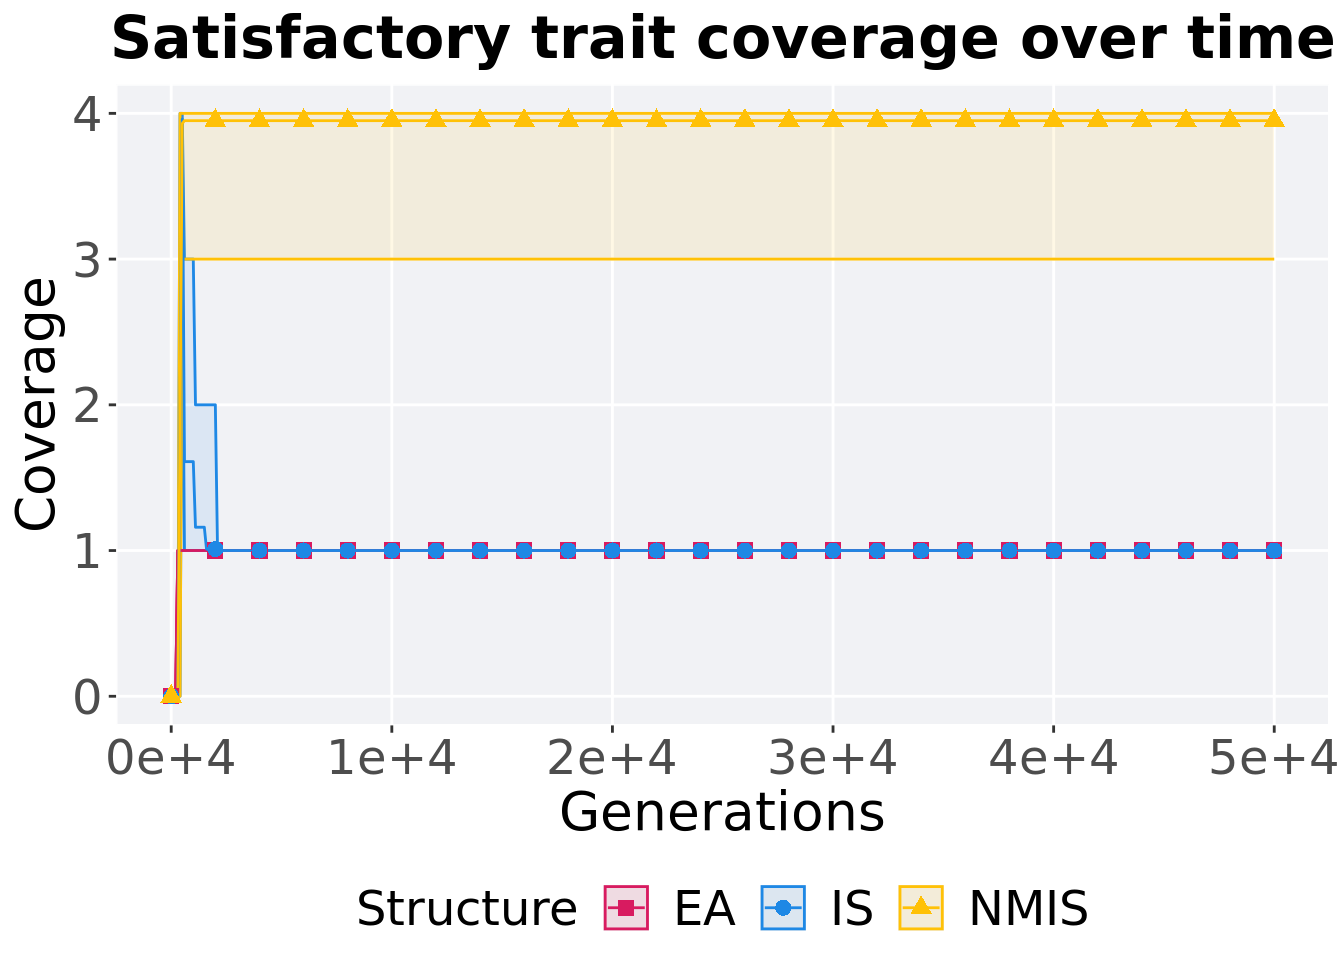
\includegraphics{demo_files/figure-latex/con-sat-tor-ot-1.pdf}

\hypertarget{best-coverage-throughout-1}{%
\subsubsection{Best coverage throughout}\label{best-coverage-throughout-1}}

Best satisfactory trait coverage throughout 50,000 generations.

\begin{Shaded}
\begin{Highlighting}[]
\CommentTok{### best satisfactory trait coverage throughout}
\KeywordTok{filter}\NormalTok{(base_best, Diagnostic }\OperatorTok{==}\StringTok{ 'CONTRADICTORY_OBJECTIVES'} \OperatorTok{&}\StringTok{ `}\DataTypeTok{Selection}\CharTok{\textbackslash{}n}\DataTypeTok{Scheme}\StringTok{`} \OperatorTok{==}\StringTok{ 'TOURNAMENT'} \OperatorTok{&}\StringTok{ }\NormalTok{VAR }\OperatorTok{==}\StringTok{ 'pop_sat_cov'}\NormalTok{) }\OperatorTok
\StringTok{  }\KeywordTok{ggplot}\NormalTok{(., }\KeywordTok{aes}\NormalTok{(}\DataTypeTok{x =}\NormalTok{ Structure, }\DataTypeTok{y =}\NormalTok{ VAL, }\DataTypeTok{color =}\NormalTok{ Structure, }\DataTypeTok{fill =}\NormalTok{ Structure, }\DataTypeTok{shape =}\NormalTok{ Structure)) }\OperatorTok{+}
\StringTok{  }\KeywordTok{geom_flat_violin}\NormalTok{(}\DataTypeTok{position =} \KeywordTok{position_nudge}\NormalTok{(}\DataTypeTok{x =} \FloatTok{.2}\NormalTok{, }\DataTypeTok{y =} \DecValTok{0}\NormalTok{), }\DataTypeTok{scale =} \StringTok{'width'}\NormalTok{, }\DataTypeTok{alpha =} \FloatTok{0.2}\NormalTok{) }\OperatorTok{+}
\StringTok{  }\KeywordTok{geom_point}\NormalTok{(}\DataTypeTok{position =} \KeywordTok{position_jitter}\NormalTok{(}\DataTypeTok{height =} \FloatTok{.05}\NormalTok{, }\DataTypeTok{width =} \FloatTok{.05}\NormalTok{), }\DataTypeTok{size =} \FloatTok{1.5}\NormalTok{, }\DataTypeTok{alpha =} \FloatTok{1.0}\NormalTok{) }\OperatorTok{+}
\StringTok{  }\KeywordTok{geom_boxplot}\NormalTok{(}\DataTypeTok{color =} \StringTok{'black'}\NormalTok{, }\DataTypeTok{width =} \FloatTok{.2}\NormalTok{, }\DataTypeTok{outlier.shape =} \OtherTok{NA}\NormalTok{, }\DataTypeTok{alpha =} \FloatTok{0.0}\NormalTok{) }\OperatorTok{+}
\StringTok{  }\KeywordTok{scale_y_continuous}\NormalTok{(}
    \DataTypeTok{name=}\StringTok{"coverage"}
\NormalTok{  ) }\OperatorTok{+}
\StringTok{  }\KeywordTok{scale_x_discrete}\NormalTok{(}
    \DataTypeTok{name=}\StringTok{"Structure"}
\NormalTok{  )}\OperatorTok{+}
\StringTok{  }\KeywordTok{scale_shape_manual}\NormalTok{(}\DataTypeTok{values=}\NormalTok{SHAPE)}\OperatorTok{+}
\StringTok{  }\KeywordTok{scale_colour_manual}\NormalTok{(}\DataTypeTok{values =}\NormalTok{ cb_palette, ) }\OperatorTok{+}
\StringTok{  }\KeywordTok{scale_fill_manual}\NormalTok{(}\DataTypeTok{values =}\NormalTok{ cb_palette) }\OperatorTok{+}
\StringTok{  }\KeywordTok{ggtitle}\NormalTok{(}\StringTok{'Best satisfactory trait coverage'}\NormalTok{)}\OperatorTok{+}
\StringTok{  }\NormalTok{p_theme }\OperatorTok{+}\StringTok{ }\KeywordTok{coord_flip}\NormalTok{()}
\end{Highlighting}
\end{Shaded}

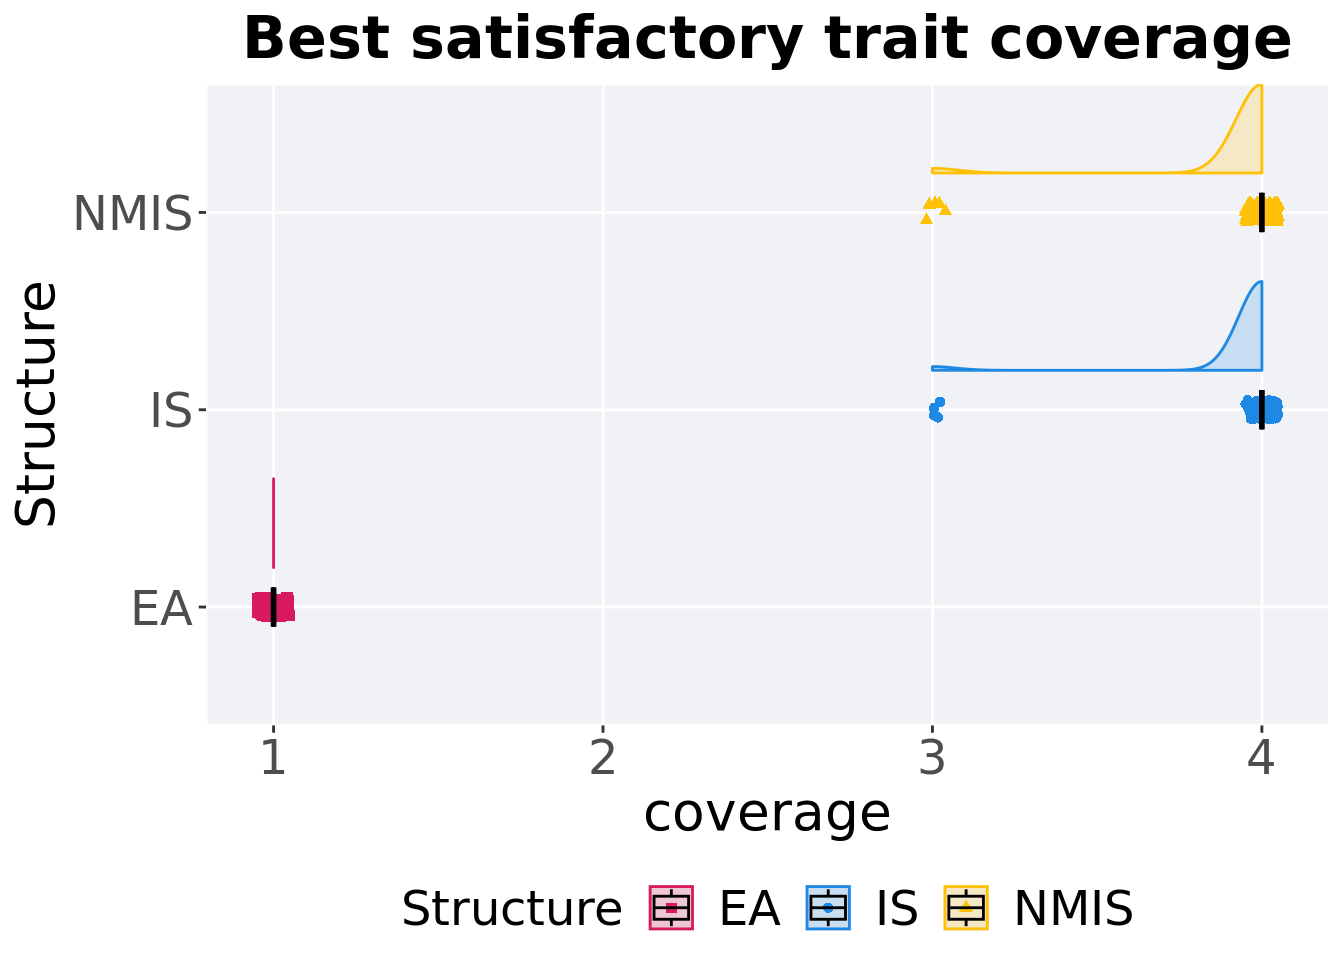
\includegraphics{demo_files/figure-latex/con-sat-tor-bst-1.pdf}

\hypertarget{stats-11}{%
\paragraph{Stats}\label{stats-11}}

Summary statistics for the best satisfactory trait coverage.

\begin{Shaded}
\begin{Highlighting}[]
\CommentTok{### best}
\NormalTok{coverage =}\StringTok{ }\KeywordTok{filter}\NormalTok{(base_best, Diagnostic }\OperatorTok{==}\StringTok{ 'CONTRADICTORY_OBJECTIVES'} \OperatorTok{&}\StringTok{ `}\DataTypeTok{Selection}\CharTok{\textbackslash{}n}\DataTypeTok{Scheme}\StringTok{`} \OperatorTok{==}\StringTok{ 'TOURNAMENT'} \OperatorTok{&}\StringTok{ }\NormalTok{VAR }\OperatorTok{==}\StringTok{ 'pop_sat_cov'}\NormalTok{)}
\NormalTok{coverage }\OperatorTok
\StringTok{  }\KeywordTok{group_by}\NormalTok{(Structure) }\OperatorTok
\StringTok{  }\NormalTok{dplyr}\OperatorTok{::}\KeywordTok{summarise}\NormalTok{(}
    \DataTypeTok{count =} \KeywordTok{n}\NormalTok{(),}
    \DataTypeTok{na_cnt =} \KeywordTok{sum}\NormalTok{(}\KeywordTok{is.na}\NormalTok{(VAL)),}
    \DataTypeTok{min =} \KeywordTok{min}\NormalTok{(VAL, }\DataTypeTok{na.rm =} \OtherTok{TRUE}\NormalTok{),}
    \DataTypeTok{median =} \KeywordTok{median}\NormalTok{(VAL, }\DataTypeTok{na.rm =} \OtherTok{TRUE}\NormalTok{),}
    \DataTypeTok{mean =} \KeywordTok{mean}\NormalTok{(VAL, }\DataTypeTok{na.rm =} \OtherTok{TRUE}\NormalTok{),}
    \DataTypeTok{max =} \KeywordTok{max}\NormalTok{(VAL, }\DataTypeTok{na.rm =} \OtherTok{TRUE}\NormalTok{),}
    \DataTypeTok{IQR =} \KeywordTok{IQR}\NormalTok{(VAL, }\DataTypeTok{na.rm =} \OtherTok{TRUE}\NormalTok{)}
\NormalTok{  )}
\end{Highlighting}
\end{Shaded}

\begin{verbatim}
## # A tibble: 3 x 8
##   Structure count na_cnt   min median  mean   max   IQR
##   <fct>     <int>  <int> <dbl>  <dbl> <dbl> <dbl> <dbl>
## 1 EA          100      0     1      1  1        1     0
## 2 IS          100      0     3      4  3.96     4     0
## 3 NMIS        100      0     3      4  3.95     4     0
\end{verbatim}

Kruskal--Wallis test provides evidence of difference among satisfactory trait coverage.

\begin{Shaded}
\begin{Highlighting}[]
\KeywordTok{kruskal.test}\NormalTok{(VAL }\OperatorTok{~}\StringTok{ }\NormalTok{Structure, }\DataTypeTok{data =}\NormalTok{ coverage)}
\end{Highlighting}
\end{Shaded}

\begin{verbatim}
## 
##  Kruskal-Wallis rank sum test
## 
## data:  VAL by Structure
## Kruskal-Wallis chi-squared = 282.81, df = 2, p-value < 2.2e-16
\end{verbatim}

Results for post-hoc Wilcoxon rank-sum test with a Bonferroni correction on satisfactory trait coverage.

\begin{Shaded}
\begin{Highlighting}[]
\KeywordTok{pairwise.wilcox.test}\NormalTok{(}\DataTypeTok{x =}\NormalTok{ coverage}\OperatorTok{$}\NormalTok{VAL, }\DataTypeTok{g =}\NormalTok{ coverage}\OperatorTok{$}\NormalTok{Structure, }\DataTypeTok{p.adjust.method =} \StringTok{"bonferroni"}\NormalTok{,}
                     \DataTypeTok{paired =} \OtherTok{FALSE}\NormalTok{, }\DataTypeTok{conf.int =} \OtherTok{FALSE}\NormalTok{, }\DataTypeTok{alternative =} \StringTok{'g'}\NormalTok{)}
\end{Highlighting}
\end{Shaded}

\begin{verbatim}
## 
##  Pairwise comparisons using Wilcoxon rank sum test with continuity correction 
## 
## data:  coverage$VAL and coverage$Structure 
## 
##      EA     IS
## IS   <2e-16 - 
## NMIS <2e-16 1 
## 
## P value adjustment method: bonferroni
\end{verbatim}

\hypertarget{end-of-50000-generations-2}{%
\subsubsection{End of 50,000 generations}\label{end-of-50000-generations-2}}

Satisfactory trait coverage in the population at the end of 50,000 generations.

\begin{Shaded}
\begin{Highlighting}[]
\CommentTok{### end of run}
\KeywordTok{filter}\NormalTok{(base_over_time, Diagnostic }\OperatorTok{==}\StringTok{ 'CONTRADICTORY_OBJECTIVES'} \OperatorTok{&}\StringTok{ `}\DataTypeTok{Selection}\CharTok{\textbackslash{}n}\DataTypeTok{Scheme}\StringTok{`} \OperatorTok{==}\StringTok{ 'TOURNAMENT'} \OperatorTok{&}\StringTok{ }\NormalTok{Generations }\OperatorTok{==}\StringTok{ }\DecValTok{50000}\NormalTok{) }\OperatorTok
\StringTok{  }\KeywordTok{ggplot}\NormalTok{(., }\KeywordTok{aes}\NormalTok{(}\DataTypeTok{x =}\NormalTok{ Structure, }\DataTypeTok{y =}\NormalTok{ pop_sat_cov, }\DataTypeTok{color =}\NormalTok{ Structure, }\DataTypeTok{fill =}\NormalTok{ Structure, }\DataTypeTok{shape =}\NormalTok{ Structure)) }\OperatorTok{+}
\StringTok{  }\KeywordTok{geom_flat_violin}\NormalTok{(}\DataTypeTok{position =} \KeywordTok{position_nudge}\NormalTok{(}\DataTypeTok{x =} \FloatTok{.2}\NormalTok{, }\DataTypeTok{y =} \DecValTok{0}\NormalTok{), }\DataTypeTok{scale =} \StringTok{'width'}\NormalTok{, }\DataTypeTok{alpha =} \FloatTok{0.3}\NormalTok{) }\OperatorTok{+}
\StringTok{  }\KeywordTok{geom_point}\NormalTok{(}\DataTypeTok{position =} \KeywordTok{position_jitter}\NormalTok{(}\DataTypeTok{height =} \FloatTok{.05}\NormalTok{, }\DataTypeTok{width =} \FloatTok{.05}\NormalTok{), }\DataTypeTok{size =} \FloatTok{1.5}\NormalTok{, }\DataTypeTok{alpha =} \FloatTok{0.5}\NormalTok{) }\OperatorTok{+}
\StringTok{  }\KeywordTok{geom_boxplot}\NormalTok{(}\DataTypeTok{color =} \StringTok{'black'}\NormalTok{, }\DataTypeTok{width =} \FloatTok{.2}\NormalTok{, }\DataTypeTok{outlier.shape =} \OtherTok{NA}\NormalTok{, }\DataTypeTok{alpha =} \FloatTok{0.0}\NormalTok{) }\OperatorTok{+}
\StringTok{  }\KeywordTok{scale_shape_manual}\NormalTok{(}\DataTypeTok{values=}\NormalTok{SHAPE)}\OperatorTok{+}
\StringTok{  }\KeywordTok{scale_y_continuous}\NormalTok{(}
    \DataTypeTok{name=}\StringTok{"Coverage"}
\NormalTok{  ) }\OperatorTok{+}
\StringTok{  }\KeywordTok{scale_x_discrete}\NormalTok{(}
    \DataTypeTok{name=}\StringTok{"Structure"}
\NormalTok{  ) }\OperatorTok{+}
\StringTok{  }\KeywordTok{scale_colour_manual}\NormalTok{(}\DataTypeTok{values =}\NormalTok{ cb_palette) }\OperatorTok{+}
\StringTok{  }\KeywordTok{scale_fill_manual}\NormalTok{(}\DataTypeTok{values =}\NormalTok{ cb_palette) }\OperatorTok{+}
\StringTok{  }\KeywordTok{ggtitle}\NormalTok{(}\StringTok{'Final satisfactory trait coverage'}\NormalTok{)}\OperatorTok{+}
\StringTok{  }\NormalTok{p_theme }\OperatorTok{+}\StringTok{ }\KeywordTok{coord_flip}\NormalTok{()}
\end{Highlighting}
\end{Shaded}

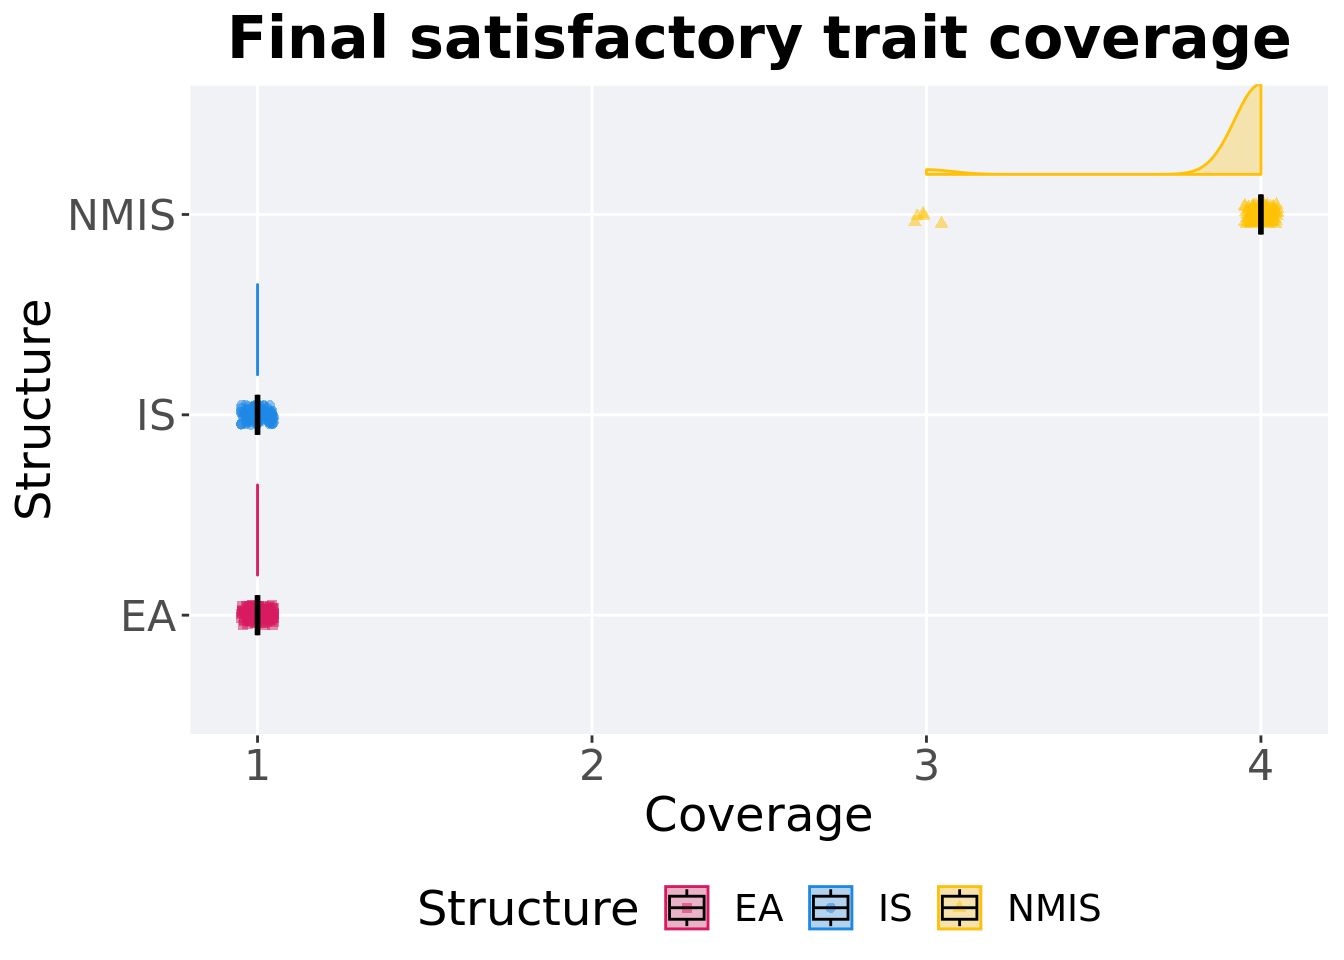
\includegraphics{demo_files/figure-latex/con-sat-tor-end-1.pdf}

\hypertarget{stats-12}{%
\paragraph{Stats}\label{stats-12}}

Summary statistics for satisfactory trait coverage in the population at the end of 50,000 generations.

\begin{Shaded}
\begin{Highlighting}[]
\CommentTok{### end of run}
\NormalTok{coverage =}\StringTok{ }\KeywordTok{filter}\NormalTok{(base_over_time, Diagnostic }\OperatorTok{==}\StringTok{ 'CONTRADICTORY_OBJECTIVES'} \OperatorTok{&}\StringTok{ `}\DataTypeTok{Selection}\CharTok{\textbackslash{}n}\DataTypeTok{Scheme}\StringTok{`} \OperatorTok{==}\StringTok{ 'TOURNAMENT'} \OperatorTok{&}\StringTok{ }\NormalTok{Generations }\OperatorTok{==}\StringTok{ }\DecValTok{50000}\NormalTok{)}
\NormalTok{coverage }\OperatorTok
\StringTok{  }\KeywordTok{group_by}\NormalTok{(Structure) }\OperatorTok
\StringTok{  }\NormalTok{dplyr}\OperatorTok{::}\KeywordTok{summarise}\NormalTok{(}
    \DataTypeTok{count =} \KeywordTok{n}\NormalTok{(),}
    \DataTypeTok{na_cnt =} \KeywordTok{sum}\NormalTok{(}\KeywordTok{is.na}\NormalTok{(pop_sat_cov)),}
    \DataTypeTok{min =} \KeywordTok{min}\NormalTok{(pop_sat_cov, }\DataTypeTok{na.rm =} \OtherTok{TRUE}\NormalTok{),}
    \DataTypeTok{median =} \KeywordTok{median}\NormalTok{(pop_sat_cov, }\DataTypeTok{na.rm =} \OtherTok{TRUE}\NormalTok{),}
    \DataTypeTok{mean =} \KeywordTok{mean}\NormalTok{(pop_sat_cov, }\DataTypeTok{na.rm =} \OtherTok{TRUE}\NormalTok{),}
    \DataTypeTok{max =} \KeywordTok{max}\NormalTok{(pop_sat_cov, }\DataTypeTok{na.rm =} \OtherTok{TRUE}\NormalTok{),}
    \DataTypeTok{IQR =} \KeywordTok{IQR}\NormalTok{(pop_sat_cov, }\DataTypeTok{na.rm =} \OtherTok{TRUE}\NormalTok{)}
\NormalTok{  )}
\end{Highlighting}
\end{Shaded}

\begin{verbatim}
## # A tibble: 3 x 8
##   Structure count na_cnt   min median  mean   max   IQR
##   <fct>     <int>  <int> <int>  <dbl> <dbl> <int> <dbl>
## 1 EA          100      0     1      1  1        1     0
## 2 IS          100      0     1      1  1        1     0
## 3 NMIS        100      0     3      4  3.95     4     0
\end{verbatim}

Kruskal--Wallis test provides evidence of difference among satisfactory trait coverage in the population at the end of 50,000 generations.

\begin{Shaded}
\begin{Highlighting}[]
\KeywordTok{kruskal.test}\NormalTok{(pop_sat_cov }\OperatorTok{~}\StringTok{ }\NormalTok{Structure, }\DataTypeTok{data =}\NormalTok{ coverage)}
\end{Highlighting}
\end{Shaded}

\begin{verbatim}
## 
##  Kruskal-Wallis rank sum test
## 
## data:  pop_sat_cov by Structure
## Kruskal-Wallis chi-squared = 296.65, df = 2, p-value < 2.2e-16
\end{verbatim}

Results for post-hoc Wilcoxon rank-sum test with a Bonferroni correction on satisfactory trait coverage in the population at the end of 50,000 generations.

\begin{Shaded}
\begin{Highlighting}[]
\KeywordTok{pairwise.wilcox.test}\NormalTok{(}\DataTypeTok{x =}\NormalTok{ coverage}\OperatorTok{$}\NormalTok{pop_sat_cov, }\DataTypeTok{g =}\NormalTok{ coverage}\OperatorTok{$}\NormalTok{Structure, }\DataTypeTok{p.adjust.method =} \StringTok{"bonferroni"}\NormalTok{,}
                     \DataTypeTok{paired =} \OtherTok{FALSE}\NormalTok{, }\DataTypeTok{conf.int =} \OtherTok{FALSE}\NormalTok{, }\DataTypeTok{alternative =} \StringTok{'g'}\NormalTok{)}
\end{Highlighting}
\end{Shaded}

\begin{verbatim}
## 
##  Pairwise comparisons using Wilcoxon rank sum test with continuity correction 
## 
## data:  coverage$pop_sat_cov and coverage$Structure 
## 
##      EA     IS    
## IS   1      -     
## NMIS <2e-16 <2e-16
## 
## P value adjustment method: bonferroni
\end{verbatim}

\hypertarget{activation-gene-coverage-1}{%
\subsection{Activation gene coverage}\label{activation-gene-coverage-1}}

Activation gene coverage analysis.

\hypertarget{coverage-over-time-3}{%
\subsubsection{Coverage over time}\label{coverage-over-time-3}}

Activation gene coverage over time.

\begin{Shaded}
\begin{Highlighting}[]
\CommentTok{# data for lines and shading on plots}
\NormalTok{lines =}\StringTok{ }\KeywordTok{filter}\NormalTok{(base_over_time, Diagnostic }\OperatorTok{==}\StringTok{ 'CONTRADICTORY_OBJECTIVES'} \OperatorTok{&}\StringTok{ `}\DataTypeTok{Selection}\CharTok{\textbackslash{}n}\DataTypeTok{Scheme}\StringTok{`} \OperatorTok{==}\StringTok{ 'TOURNAMENT'}\NormalTok{) }\OperatorTok
\StringTok{  }\KeywordTok{group_by}\NormalTok{(Structure, Generations) }\OperatorTok
\StringTok{  }\NormalTok{dplyr}\OperatorTok{::}\KeywordTok{summarise}\NormalTok{(}
    \DataTypeTok{min =} \KeywordTok{min}\NormalTok{(pop_act_cov),}
    \DataTypeTok{mean =} \KeywordTok{mean}\NormalTok{(pop_act_cov),}
    \DataTypeTok{max =} \KeywordTok{max}\NormalTok{(pop_act_cov)}
\NormalTok{  )}
\end{Highlighting}
\end{Shaded}

\begin{verbatim}
## `summarise()` has grouped output by 'Structure'. You can override using the
## `.groups` argument.
\end{verbatim}

\begin{Shaded}
\begin{Highlighting}[]
\KeywordTok{ggplot}\NormalTok{(lines, }\KeywordTok{aes}\NormalTok{(}\DataTypeTok{x=}\NormalTok{Generations, }\DataTypeTok{y=}\NormalTok{mean, }\DataTypeTok{group =}\NormalTok{ Structure, }\DataTypeTok{fill =}\NormalTok{ Structure, }\DataTypeTok{color =}\NormalTok{ Structure, }\DataTypeTok{shape =}\NormalTok{ Structure)) }\OperatorTok{+}
\StringTok{  }\KeywordTok{geom_ribbon}\NormalTok{(}\KeywordTok{aes}\NormalTok{(}\DataTypeTok{ymin =}\NormalTok{ min, }\DataTypeTok{ymax =}\NormalTok{ max), }\DataTypeTok{alpha =} \FloatTok{0.1}\NormalTok{) }\OperatorTok{+}
\StringTok{  }\KeywordTok{geom_line}\NormalTok{(}\DataTypeTok{size =} \FloatTok{0.5}\NormalTok{) }\OperatorTok{+}
\StringTok{  }\KeywordTok{geom_point}\NormalTok{(}\DataTypeTok{data =} \KeywordTok{filter}\NormalTok{(lines, Generations }\OperatorTok\StringTok{ }\DecValTok{2000} \OperatorTok{==}\StringTok{ }\DecValTok{0}\NormalTok{), }\DataTypeTok{size =} \FloatTok{1.5}\NormalTok{, }\DataTypeTok{stroke =} \FloatTok{2.0}\NormalTok{, }\DataTypeTok{alpha =} \FloatTok{1.0}\NormalTok{) }\OperatorTok{+}
\StringTok{  }\KeywordTok{scale_y_continuous}\NormalTok{(}
    \DataTypeTok{name=}\StringTok{"Coverage"}
\NormalTok{  ) }\OperatorTok{+}
\StringTok{  }\KeywordTok{scale_x_continuous}\NormalTok{(}
    \DataTypeTok{name=}\StringTok{"Generations"}\NormalTok{,}
    \DataTypeTok{limits=}\KeywordTok{c}\NormalTok{(}\DecValTok{0}\NormalTok{, }\DecValTok{50000}\NormalTok{),}
    \DataTypeTok{breaks=}\KeywordTok{c}\NormalTok{(}\DecValTok{0}\NormalTok{, }\DecValTok{10000}\NormalTok{, }\DecValTok{20000}\NormalTok{, }\DecValTok{30000}\NormalTok{, }\DecValTok{40000}\NormalTok{, }\DecValTok{50000}\NormalTok{),}
    \DataTypeTok{labels=}\KeywordTok{c}\NormalTok{(}\StringTok{"0e+4"}\NormalTok{, }\StringTok{"1e+4"}\NormalTok{, }\StringTok{"2e+4"}\NormalTok{, }\StringTok{"3e+4"}\NormalTok{, }\StringTok{"4e+4"}\NormalTok{, }\StringTok{"5e+4"}\NormalTok{)}

\NormalTok{  ) }\OperatorTok{+}
\StringTok{  }\KeywordTok{scale_shape_manual}\NormalTok{(}\DataTypeTok{values=}\NormalTok{SHAPE)}\OperatorTok{+}
\StringTok{  }\KeywordTok{scale_colour_manual}\NormalTok{(}\DataTypeTok{values =}\NormalTok{ cb_palette) }\OperatorTok{+}
\StringTok{  }\KeywordTok{scale_fill_manual}\NormalTok{(}\DataTypeTok{values =}\NormalTok{ cb_palette) }\OperatorTok{+}
\StringTok{  }\KeywordTok{ggtitle}\NormalTok{(}\StringTok{'Activation gene coverage over time'}\NormalTok{)}\OperatorTok{+}
\StringTok{  }\NormalTok{p_theme}
\end{Highlighting}
\end{Shaded}

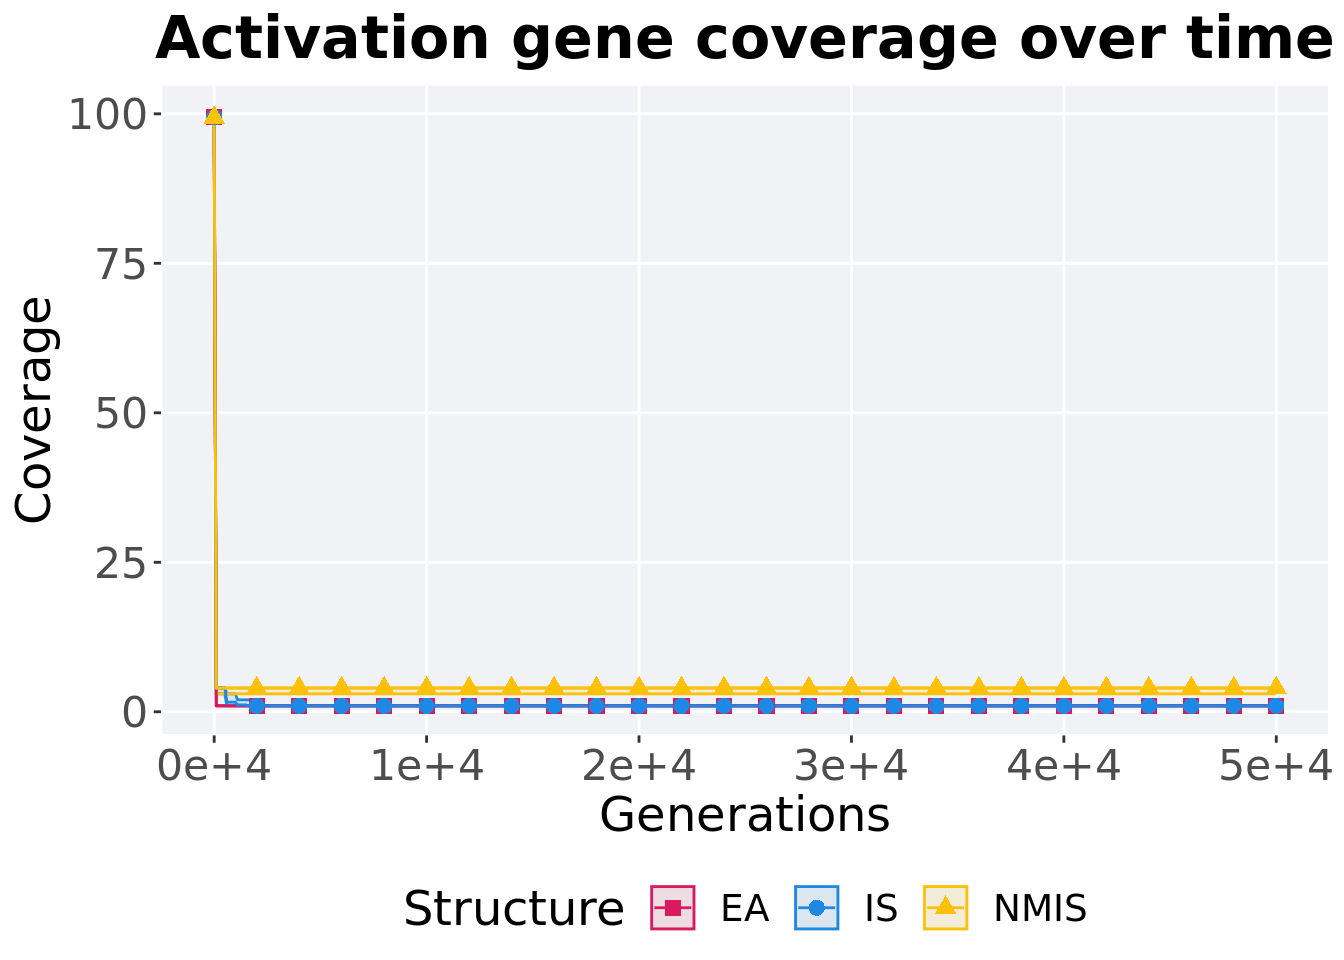
\includegraphics{demo_files/figure-latex/con-act-tor-ot-1.pdf}

\hypertarget{end-of-50000-generations-3}{%
\subsubsection{End of 50,000 generations}\label{end-of-50000-generations-3}}

Activation gene coverage in the population at the end of 50,000 generations.

\begin{Shaded}
\begin{Highlighting}[]
\CommentTok{### end of run}
\KeywordTok{filter}\NormalTok{(base_over_time, Diagnostic }\OperatorTok{==}\StringTok{ 'CONTRADICTORY_OBJECTIVES'} \OperatorTok{&}\StringTok{ `}\DataTypeTok{Selection}\CharTok{\textbackslash{}n}\DataTypeTok{Scheme}\StringTok{`} \OperatorTok{==}\StringTok{ 'TOURNAMENT'} \OperatorTok{&}\StringTok{ }\NormalTok{Generations }\OperatorTok{==}\StringTok{ }\DecValTok{50000}\NormalTok{) }\OperatorTok
\StringTok{  }\KeywordTok{ggplot}\NormalTok{(., }\KeywordTok{aes}\NormalTok{(}\DataTypeTok{x =}\NormalTok{ Structure, }\DataTypeTok{y =}\NormalTok{ pop_act_cov, }\DataTypeTok{color =}\NormalTok{ Structure, }\DataTypeTok{fill =}\NormalTok{ Structure, }\DataTypeTok{shape =}\NormalTok{ Structure)) }\OperatorTok{+}
\StringTok{  }\KeywordTok{geom_flat_violin}\NormalTok{(}\DataTypeTok{position =} \KeywordTok{position_nudge}\NormalTok{(}\DataTypeTok{x =} \FloatTok{.2}\NormalTok{, }\DataTypeTok{y =} \DecValTok{0}\NormalTok{), }\DataTypeTok{scale =} \StringTok{'width'}\NormalTok{, }\DataTypeTok{alpha =} \FloatTok{0.3}\NormalTok{) }\OperatorTok{+}
\StringTok{  }\KeywordTok{geom_point}\NormalTok{(}\DataTypeTok{position =} \KeywordTok{position_jitter}\NormalTok{(}\DataTypeTok{height =} \FloatTok{.05}\NormalTok{, }\DataTypeTok{width =} \FloatTok{.05}\NormalTok{), }\DataTypeTok{size =} \FloatTok{1.5}\NormalTok{, }\DataTypeTok{alpha =} \FloatTok{0.5}\NormalTok{) }\OperatorTok{+}
\StringTok{  }\KeywordTok{geom_boxplot}\NormalTok{(}\DataTypeTok{color =} \StringTok{'black'}\NormalTok{, }\DataTypeTok{width =} \FloatTok{.2}\NormalTok{, }\DataTypeTok{outlier.shape =} \OtherTok{NA}\NormalTok{, }\DataTypeTok{alpha =} \FloatTok{0.0}\NormalTok{) }\OperatorTok{+}
\StringTok{  }\KeywordTok{scale_shape_manual}\NormalTok{(}\DataTypeTok{values=}\NormalTok{SHAPE)}\OperatorTok{+}
\StringTok{  }\KeywordTok{scale_y_continuous}\NormalTok{(}
    \DataTypeTok{name=}\StringTok{"Coverage"}
\NormalTok{  ) }\OperatorTok{+}
\StringTok{  }\KeywordTok{scale_x_discrete}\NormalTok{(}
    \DataTypeTok{name=}\StringTok{"Structure"}
\NormalTok{  ) }\OperatorTok{+}
\StringTok{  }\KeywordTok{scale_colour_manual}\NormalTok{(}\DataTypeTok{values =}\NormalTok{ cb_palette) }\OperatorTok{+}
\StringTok{  }\KeywordTok{scale_fill_manual}\NormalTok{(}\DataTypeTok{values =}\NormalTok{ cb_palette) }\OperatorTok{+}
\StringTok{  }\KeywordTok{ggtitle}\NormalTok{(}\StringTok{'Final activation gene coverage'}\NormalTok{)}\OperatorTok{+}
\StringTok{  }\NormalTok{p_theme }\OperatorTok{+}\StringTok{ }\KeywordTok{coord_flip}\NormalTok{()}
\end{Highlighting}
\end{Shaded}

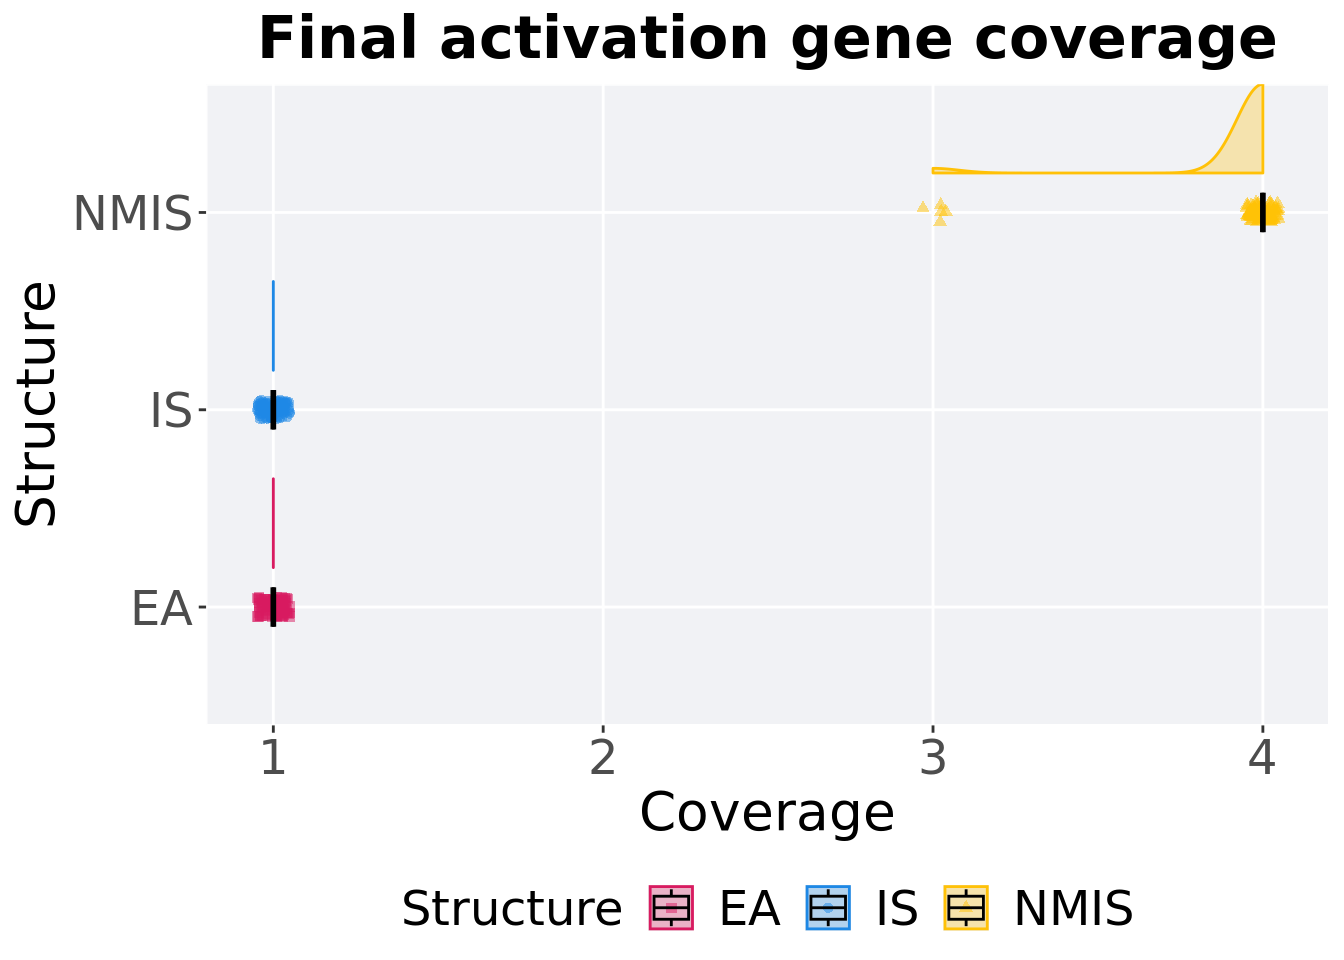
\includegraphics{demo_files/figure-latex/con-act-tor-end-1.pdf}

\hypertarget{stats-13}{%
\paragraph{Stats}\label{stats-13}}

Summary statistics for activation gene coverage.

\begin{Shaded}
\begin{Highlighting}[]
\NormalTok{coverage =}\StringTok{ }\KeywordTok{filter}\NormalTok{(base_over_time, Diagnostic }\OperatorTok{==}\StringTok{ 'CONTRADICTORY_OBJECTIVES'} \OperatorTok{&}\StringTok{ `}\DataTypeTok{Selection}\CharTok{\textbackslash{}n}\DataTypeTok{Scheme}\StringTok{`} \OperatorTok{==}\StringTok{ 'TOURNAMENT'} \OperatorTok{&}\StringTok{ }\NormalTok{Generations }\OperatorTok{==}\StringTok{ }\DecValTok{50000}\NormalTok{)}
\NormalTok{coverage }\OperatorTok
\StringTok{  }\KeywordTok{group_by}\NormalTok{(Structure) }\OperatorTok
\StringTok{  }\NormalTok{dplyr}\OperatorTok{::}\KeywordTok{summarise}\NormalTok{(}
    \DataTypeTok{count =} \KeywordTok{n}\NormalTok{(),}
    \DataTypeTok{na_cnt =} \KeywordTok{sum}\NormalTok{(}\KeywordTok{is.na}\NormalTok{(pop_act_cov)),}
    \DataTypeTok{min =} \KeywordTok{min}\NormalTok{(pop_act_cov, }\DataTypeTok{na.rm =} \OtherTok{TRUE}\NormalTok{),}
    \DataTypeTok{median =} \KeywordTok{median}\NormalTok{(pop_act_cov, }\DataTypeTok{na.rm =} \OtherTok{TRUE}\NormalTok{),}
    \DataTypeTok{mean =} \KeywordTok{mean}\NormalTok{(pop_act_cov, }\DataTypeTok{na.rm =} \OtherTok{TRUE}\NormalTok{),}
    \DataTypeTok{max =} \KeywordTok{max}\NormalTok{(pop_act_cov, }\DataTypeTok{na.rm =} \OtherTok{TRUE}\NormalTok{),}
    \DataTypeTok{IQR =} \KeywordTok{IQR}\NormalTok{(pop_act_cov, }\DataTypeTok{na.rm =} \OtherTok{TRUE}\NormalTok{)}
\NormalTok{  )}
\end{Highlighting}
\end{Shaded}

\begin{verbatim}
## # A tibble: 3 x 8
##   Structure count na_cnt   min median  mean   max   IQR
##   <fct>     <int>  <int> <int>  <dbl> <dbl> <int> <dbl>
## 1 EA          100      0     1      1  1        1     0
## 2 IS          100      0     1      1  1        1     0
## 3 NMIS        100      0     3      4  3.95     4     0
\end{verbatim}

Kruskal--Wallis test provides evidence of difference among activation gene coverage.

\begin{Shaded}
\begin{Highlighting}[]
\KeywordTok{kruskal.test}\NormalTok{(pop_act_cov }\OperatorTok{~}\StringTok{ }\NormalTok{Structure, }\DataTypeTok{data =}\NormalTok{ coverage)}
\end{Highlighting}
\end{Shaded}

\begin{verbatim}
## 
##  Kruskal-Wallis rank sum test
## 
## data:  pop_act_cov by Structure
## Kruskal-Wallis chi-squared = 296.65, df = 2, p-value < 2.2e-16
\end{verbatim}

Results for post-hoc Wilcoxon rank-sum test with a Bonferroni correction on activation gene coverage.

\begin{Shaded}
\begin{Highlighting}[]
\KeywordTok{pairwise.wilcox.test}\NormalTok{(}\DataTypeTok{x =}\NormalTok{ coverage}\OperatorTok{$}\NormalTok{pop_act_cov, }\DataTypeTok{g =}\NormalTok{ coverage}\OperatorTok{$}\NormalTok{Structure, }\DataTypeTok{p.adjust.method =} \StringTok{"bonferroni"}\NormalTok{,}
                     \DataTypeTok{paired =} \OtherTok{FALSE}\NormalTok{, }\DataTypeTok{conf.int =} \OtherTok{FALSE}\NormalTok{, }\DataTypeTok{alternative =} \StringTok{'g'}\NormalTok{)}
\end{Highlighting}
\end{Shaded}

\begin{verbatim}
## 
##  Pairwise comparisons using Wilcoxon rank sum test with continuity correction 
## 
## data:  coverage$pop_act_cov and coverage$Structure 
## 
##      EA     IS    
## IS   1      -     
## NMIS <2e-16 <2e-16
## 
## P value adjustment method: bonferroni
\end{verbatim}

\hypertarget{lexicase-selection-2}{%
\section{Lexicase selection}\label{lexicase-selection-2}}

Here we analyze how the different population structures affect standard lexicase selection on the contradictory objectives diagnostic.

\hypertarget{satisfactory-trait-coverage-2}{%
\subsection{Satisfactory trait coverage}\label{satisfactory-trait-coverage-2}}

Satisfactory trait coverage analysis.

\hypertarget{coverage-over-time-4}{%
\subsubsection{Coverage over time}\label{coverage-over-time-4}}

Satisfactory trait coverage over time.

\begin{Shaded}
\begin{Highlighting}[]
\NormalTok{lines =}\StringTok{ }\KeywordTok{filter}\NormalTok{(base_over_time, Diagnostic }\OperatorTok{==}\StringTok{ 'CONTRADICTORY_OBJECTIVES'} \OperatorTok{&}\StringTok{ `}\DataTypeTok{Selection}\CharTok{\textbackslash{}n}\DataTypeTok{Scheme}\StringTok{`} \OperatorTok{==}\StringTok{ 'LEXICASE'}\NormalTok{) }\OperatorTok
\StringTok{  }\KeywordTok{group_by}\NormalTok{(Structure, Generations) }\OperatorTok
\StringTok{  }\NormalTok{dplyr}\OperatorTok{::}\KeywordTok{summarise}\NormalTok{(}
    \DataTypeTok{min =} \KeywordTok{min}\NormalTok{(pop_sat_cov),}
    \DataTypeTok{mean =} \KeywordTok{mean}\NormalTok{(pop_sat_cov),}
    \DataTypeTok{max =} \KeywordTok{max}\NormalTok{(pop_sat_cov)}
\NormalTok{  )}
\end{Highlighting}
\end{Shaded}

\begin{verbatim}
## `summarise()` has grouped output by 'Structure'. You can override using the
## `.groups` argument.
\end{verbatim}

\begin{Shaded}
\begin{Highlighting}[]
\KeywordTok{ggplot}\NormalTok{(lines, }\KeywordTok{aes}\NormalTok{(}\DataTypeTok{x=}\NormalTok{Generations, }\DataTypeTok{y=}\NormalTok{mean, }\DataTypeTok{group =}\NormalTok{ Structure, }\DataTypeTok{fill =}\NormalTok{ Structure, }\DataTypeTok{color =}\NormalTok{ Structure, }\DataTypeTok{shape =}\NormalTok{ Structure)) }\OperatorTok{+}
\StringTok{  }\KeywordTok{geom_ribbon}\NormalTok{(}\KeywordTok{aes}\NormalTok{(}\DataTypeTok{ymin =}\NormalTok{ min, }\DataTypeTok{ymax =}\NormalTok{ max), }\DataTypeTok{alpha =} \FloatTok{0.1}\NormalTok{) }\OperatorTok{+}
\StringTok{  }\KeywordTok{geom_line}\NormalTok{(}\DataTypeTok{size =} \FloatTok{0.5}\NormalTok{) }\OperatorTok{+}
\StringTok{  }\KeywordTok{geom_point}\NormalTok{(}\DataTypeTok{data =} \KeywordTok{filter}\NormalTok{(lines, Generations }\OperatorTok\StringTok{ }\DecValTok{2000} \OperatorTok{==}\StringTok{ }\DecValTok{0}\NormalTok{), }\DataTypeTok{size =} \FloatTok{1.5}\NormalTok{, }\DataTypeTok{stroke =} \FloatTok{2.0}\NormalTok{, }\DataTypeTok{alpha =} \FloatTok{1.0}\NormalTok{) }\OperatorTok{+}
\StringTok{  }\KeywordTok{scale_y_continuous}\NormalTok{(}
    \DataTypeTok{name=}\StringTok{"Coverage"}
\NormalTok{  ) }\OperatorTok{+}
\StringTok{  }\KeywordTok{scale_x_continuous}\NormalTok{(}
    \DataTypeTok{name=}\StringTok{"Generations"}\NormalTok{,}
    \DataTypeTok{limits=}\KeywordTok{c}\NormalTok{(}\DecValTok{0}\NormalTok{, }\DecValTok{50000}\NormalTok{),}
    \DataTypeTok{breaks=}\KeywordTok{c}\NormalTok{(}\DecValTok{0}\NormalTok{, }\DecValTok{10000}\NormalTok{, }\DecValTok{20000}\NormalTok{, }\DecValTok{30000}\NormalTok{, }\DecValTok{40000}\NormalTok{, }\DecValTok{50000}\NormalTok{),}
    \DataTypeTok{labels=}\KeywordTok{c}\NormalTok{(}\StringTok{"0e+4"}\NormalTok{, }\StringTok{"1e+4"}\NormalTok{, }\StringTok{"2e+4"}\NormalTok{, }\StringTok{"3e+4"}\NormalTok{, }\StringTok{"4e+4"}\NormalTok{, }\StringTok{"5e+4"}\NormalTok{)}

\NormalTok{  ) }\OperatorTok{+}
\StringTok{  }\KeywordTok{scale_shape_manual}\NormalTok{(}\DataTypeTok{values=}\NormalTok{SHAPE)}\OperatorTok{+}
\StringTok{  }\KeywordTok{scale_colour_manual}\NormalTok{(}\DataTypeTok{values =}\NormalTok{ cb_palette) }\OperatorTok{+}
\StringTok{  }\KeywordTok{scale_fill_manual}\NormalTok{(}\DataTypeTok{values =}\NormalTok{ cb_palette) }\OperatorTok{+}
\StringTok{  }\KeywordTok{ggtitle}\NormalTok{(}\StringTok{'Satisfactory trait coverage over time'}\NormalTok{)}\OperatorTok{+}
\StringTok{  }\NormalTok{p_theme}
\end{Highlighting}
\end{Shaded}

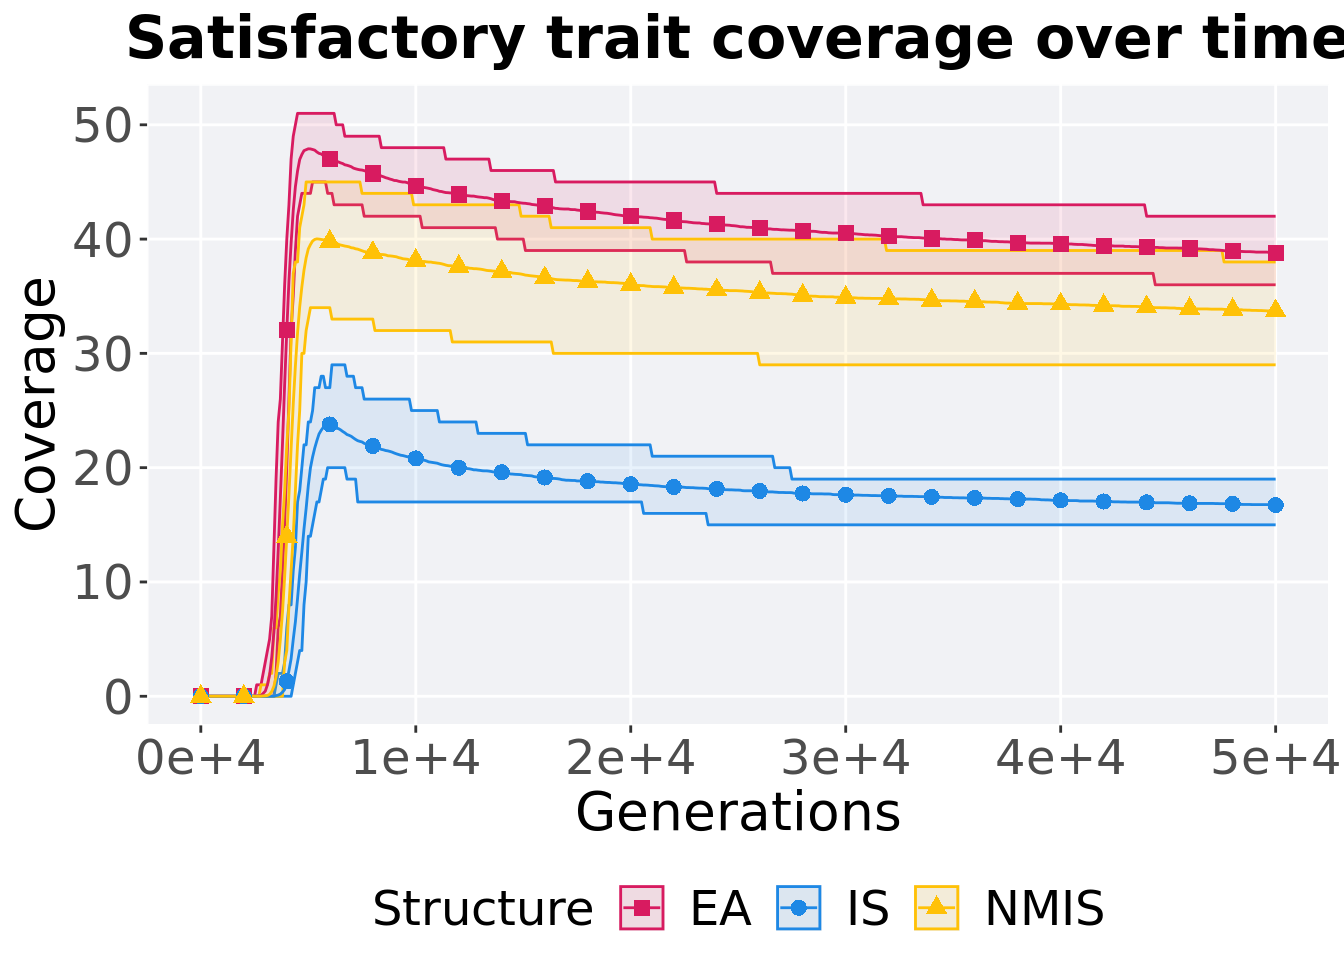
\includegraphics{demo_files/figure-latex/con-sat-lex-ot-1.pdf}

\hypertarget{best-coverage-throughout-2}{%
\subsubsection{Best coverage throughout}\label{best-coverage-throughout-2}}

Best satisfactory trait coverage throughout 50,000 generations.

\begin{Shaded}
\begin{Highlighting}[]
\CommentTok{### best satisfactory trait coverage throughout}
\KeywordTok{filter}\NormalTok{(base_best, Diagnostic }\OperatorTok{==}\StringTok{ 'CONTRADICTORY_OBJECTIVES'} \OperatorTok{&}\StringTok{ `}\DataTypeTok{Selection}\CharTok{\textbackslash{}n}\DataTypeTok{Scheme}\StringTok{`} \OperatorTok{==}\StringTok{ 'LEXICASE'} \OperatorTok{&}\StringTok{ }\NormalTok{VAR }\OperatorTok{==}\StringTok{ 'pop_sat_cov'}\NormalTok{) }\OperatorTok
\StringTok{  }\KeywordTok{ggplot}\NormalTok{(., }\KeywordTok{aes}\NormalTok{(}\DataTypeTok{x =}\NormalTok{ Structure, }\DataTypeTok{y =}\NormalTok{ VAL, }\DataTypeTok{color =}\NormalTok{ Structure, }\DataTypeTok{fill =}\NormalTok{ Structure, }\DataTypeTok{shape =}\NormalTok{ Structure)) }\OperatorTok{+}
\StringTok{  }\KeywordTok{geom_flat_violin}\NormalTok{(}\DataTypeTok{position =} \KeywordTok{position_nudge}\NormalTok{(}\DataTypeTok{x =} \FloatTok{.2}\NormalTok{, }\DataTypeTok{y =} \DecValTok{0}\NormalTok{), }\DataTypeTok{scale =} \StringTok{'width'}\NormalTok{, }\DataTypeTok{alpha =} \FloatTok{0.2}\NormalTok{) }\OperatorTok{+}
\StringTok{  }\KeywordTok{geom_point}\NormalTok{(}\DataTypeTok{position =} \KeywordTok{position_jitter}\NormalTok{(}\DataTypeTok{height =} \FloatTok{.05}\NormalTok{, }\DataTypeTok{width =} \FloatTok{.05}\NormalTok{), }\DataTypeTok{size =} \FloatTok{1.5}\NormalTok{, }\DataTypeTok{alpha =} \FloatTok{1.0}\NormalTok{) }\OperatorTok{+}
\StringTok{  }\KeywordTok{geom_boxplot}\NormalTok{(}\DataTypeTok{color =} \StringTok{'black'}\NormalTok{, }\DataTypeTok{width =} \FloatTok{.2}\NormalTok{, }\DataTypeTok{outlier.shape =} \OtherTok{NA}\NormalTok{, }\DataTypeTok{alpha =} \FloatTok{0.0}\NormalTok{) }\OperatorTok{+}
\StringTok{  }\KeywordTok{scale_y_continuous}\NormalTok{(}
    \DataTypeTok{name=}\StringTok{"coverage"}
\NormalTok{  ) }\OperatorTok{+}
\StringTok{  }\KeywordTok{scale_x_discrete}\NormalTok{(}
    \DataTypeTok{name=}\StringTok{"Structure"}
\NormalTok{  )}\OperatorTok{+}
\StringTok{  }\KeywordTok{scale_shape_manual}\NormalTok{(}\DataTypeTok{values=}\NormalTok{SHAPE)}\OperatorTok{+}
\StringTok{  }\KeywordTok{scale_colour_manual}\NormalTok{(}\DataTypeTok{values =}\NormalTok{ cb_palette, ) }\OperatorTok{+}
\StringTok{  }\KeywordTok{scale_fill_manual}\NormalTok{(}\DataTypeTok{values =}\NormalTok{ cb_palette) }\OperatorTok{+}
\StringTok{  }\KeywordTok{ggtitle}\NormalTok{(}\StringTok{'Best satisfactory trait coverage'}\NormalTok{)}\OperatorTok{+}
\StringTok{  }\NormalTok{p_theme }\OperatorTok{+}\StringTok{ }\KeywordTok{coord_flip}\NormalTok{()}
\end{Highlighting}
\end{Shaded}

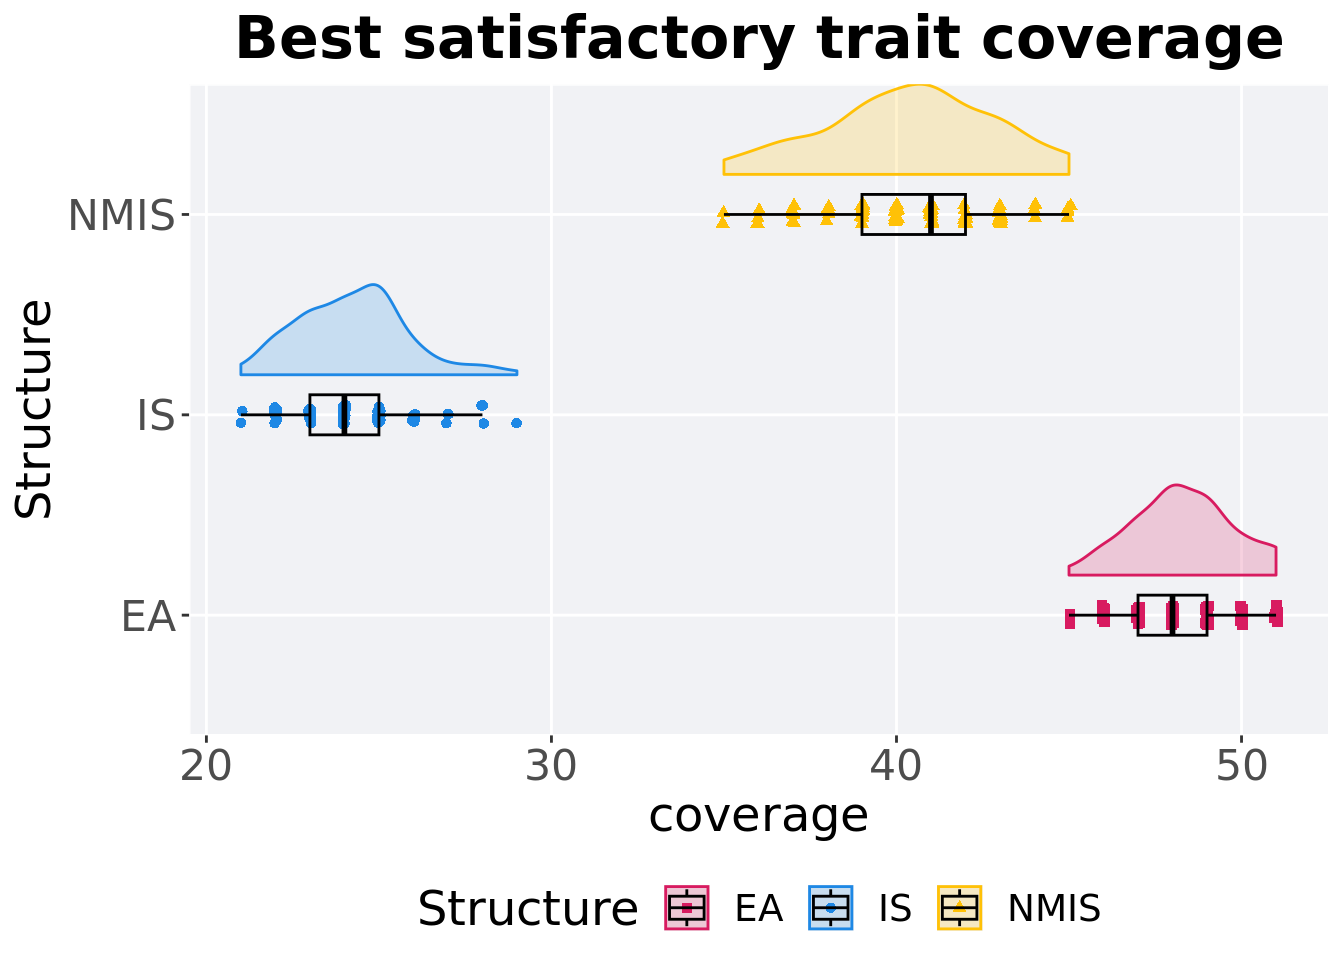
\includegraphics{demo_files/figure-latex/con-sat-lex-bst-1.pdf}

\hypertarget{stats-14}{%
\paragraph{Stats}\label{stats-14}}

Summary statistics for the best satisfactory trait coverage.

\begin{Shaded}
\begin{Highlighting}[]
\CommentTok{### best}
\NormalTok{coverage =}\StringTok{ }\KeywordTok{filter}\NormalTok{(base_best, Diagnostic }\OperatorTok{==}\StringTok{ 'CONTRADICTORY_OBJECTIVES'} \OperatorTok{&}\StringTok{ `}\DataTypeTok{Selection}\CharTok{\textbackslash{}n}\DataTypeTok{Scheme}\StringTok{`} \OperatorTok{==}\StringTok{ 'LEXICASE'} \OperatorTok{&}\StringTok{ }\NormalTok{VAR }\OperatorTok{==}\StringTok{ 'pop_sat_cov'}\NormalTok{)}
\NormalTok{coverage}\OperatorTok{$}\NormalTok{Structure =}\StringTok{ }\KeywordTok{factor}\NormalTok{(coverage}\OperatorTok{$}\NormalTok{Structure, }\DataTypeTok{levels=}\KeywordTok{c}\NormalTok{(}\StringTok{'EA'}\NormalTok{,}\StringTok{'NMIS'}\NormalTok{,}\StringTok{'IS'}\NormalTok{))}
\NormalTok{coverage }\OperatorTok
\StringTok{  }\KeywordTok{group_by}\NormalTok{(Structure) }\OperatorTok
\StringTok{  }\NormalTok{dplyr}\OperatorTok{::}\KeywordTok{summarise}\NormalTok{(}
    \DataTypeTok{count =} \KeywordTok{n}\NormalTok{(),}
    \DataTypeTok{na_cnt =} \KeywordTok{sum}\NormalTok{(}\KeywordTok{is.na}\NormalTok{(VAL)),}
    \DataTypeTok{min =} \KeywordTok{min}\NormalTok{(VAL, }\DataTypeTok{na.rm =} \OtherTok{TRUE}\NormalTok{),}
    \DataTypeTok{median =} \KeywordTok{median}\NormalTok{(VAL, }\DataTypeTok{na.rm =} \OtherTok{TRUE}\NormalTok{),}
    \DataTypeTok{mean =} \KeywordTok{mean}\NormalTok{(VAL, }\DataTypeTok{na.rm =} \OtherTok{TRUE}\NormalTok{),}
    \DataTypeTok{max =} \KeywordTok{max}\NormalTok{(VAL, }\DataTypeTok{na.rm =} \OtherTok{TRUE}\NormalTok{),}
    \DataTypeTok{IQR =} \KeywordTok{IQR}\NormalTok{(VAL, }\DataTypeTok{na.rm =} \OtherTok{TRUE}\NormalTok{)}
\NormalTok{  )}
\end{Highlighting}
\end{Shaded}

\begin{verbatim}
## # A tibble: 3 x 8
##   Structure count na_cnt   min median  mean   max   IQR
##   <fct>     <int>  <int> <dbl>  <dbl> <dbl> <dbl> <dbl>
## 1 EA          100      0    45     48  48.3    51     2
## 2 NMIS        100      0    35     41  40.4    45     3
## 3 IS          100      0    21     24  24.2    29     2
\end{verbatim}

Kruskal--Wallis test provides evidence of difference among satisfactory trait coverage.

\begin{Shaded}
\begin{Highlighting}[]
\KeywordTok{kruskal.test}\NormalTok{(VAL }\OperatorTok{~}\StringTok{ }\NormalTok{Structure, }\DataTypeTok{data =}\NormalTok{ coverage)}
\end{Highlighting}
\end{Shaded}

\begin{verbatim}
## 
##  Kruskal-Wallis rank sum test
## 
## data:  VAL by Structure
## Kruskal-Wallis chi-squared = 266.69, df = 2, p-value < 2.2e-16
\end{verbatim}

Results for post-hoc Wilcoxon rank-sum test with a Bonferroni correction on satisfactory trait coverage.

\begin{Shaded}
\begin{Highlighting}[]
\KeywordTok{pairwise.wilcox.test}\NormalTok{(}\DataTypeTok{x =}\NormalTok{ coverage}\OperatorTok{$}\NormalTok{VAL, }\DataTypeTok{g =}\NormalTok{ coverage}\OperatorTok{$}\NormalTok{Structure, }\DataTypeTok{p.adjust.method =} \StringTok{"bonferroni"}\NormalTok{,}
                     \DataTypeTok{paired =} \OtherTok{FALSE}\NormalTok{, }\DataTypeTok{conf.int =} \OtherTok{FALSE}\NormalTok{, }\DataTypeTok{alternative =} \StringTok{'l'}\NormalTok{)}
\end{Highlighting}
\end{Shaded}

\begin{verbatim}
## 
##  Pairwise comparisons using Wilcoxon rank sum test with continuity correction 
## 
## data:  coverage$VAL and coverage$Structure 
## 
##      EA     NMIS  
## NMIS <2e-16 -     
## IS   <2e-16 <2e-16
## 
## P value adjustment method: bonferroni
\end{verbatim}

\hypertarget{end-of-50000-generations-4}{%
\subsubsection{End of 50,000 generations}\label{end-of-50000-generations-4}}

Satisfactory trait coverage in the population at the end of 50,000 generations.

\begin{Shaded}
\begin{Highlighting}[]
\CommentTok{### end of run}
\KeywordTok{filter}\NormalTok{(base_over_time, Diagnostic }\OperatorTok{==}\StringTok{ 'CONTRADICTORY_OBJECTIVES'} \OperatorTok{&}\StringTok{ `}\DataTypeTok{Selection}\CharTok{\textbackslash{}n}\DataTypeTok{Scheme}\StringTok{`} \OperatorTok{==}\StringTok{ 'LEXICASE'} \OperatorTok{&}\StringTok{ }\NormalTok{Generations }\OperatorTok{==}\StringTok{ }\DecValTok{50000}\NormalTok{) }\OperatorTok
\StringTok{  }\KeywordTok{ggplot}\NormalTok{(., }\KeywordTok{aes}\NormalTok{(}\DataTypeTok{x =}\NormalTok{ Structure, }\DataTypeTok{y =}\NormalTok{ pop_sat_cov, }\DataTypeTok{color =}\NormalTok{ Structure, }\DataTypeTok{fill =}\NormalTok{ Structure, }\DataTypeTok{shape =}\NormalTok{ Structure)) }\OperatorTok{+}
\StringTok{  }\KeywordTok{geom_flat_violin}\NormalTok{(}\DataTypeTok{position =} \KeywordTok{position_nudge}\NormalTok{(}\DataTypeTok{x =} \FloatTok{.2}\NormalTok{, }\DataTypeTok{y =} \DecValTok{0}\NormalTok{), }\DataTypeTok{scale =} \StringTok{'width'}\NormalTok{, }\DataTypeTok{alpha =} \FloatTok{0.3}\NormalTok{) }\OperatorTok{+}
\StringTok{  }\KeywordTok{geom_point}\NormalTok{(}\DataTypeTok{position =} \KeywordTok{position_jitter}\NormalTok{(}\DataTypeTok{height =} \FloatTok{.05}\NormalTok{, }\DataTypeTok{width =} \FloatTok{.05}\NormalTok{), }\DataTypeTok{size =} \FloatTok{1.5}\NormalTok{, }\DataTypeTok{alpha =} \FloatTok{0.5}\NormalTok{) }\OperatorTok{+}
\StringTok{  }\KeywordTok{geom_boxplot}\NormalTok{(}\DataTypeTok{color =} \StringTok{'black'}\NormalTok{, }\DataTypeTok{width =} \FloatTok{.2}\NormalTok{, }\DataTypeTok{outlier.shape =} \OtherTok{NA}\NormalTok{, }\DataTypeTok{alpha =} \FloatTok{0.0}\NormalTok{) }\OperatorTok{+}
\StringTok{  }\KeywordTok{scale_shape_manual}\NormalTok{(}\DataTypeTok{values=}\NormalTok{SHAPE)}\OperatorTok{+}
\StringTok{  }\KeywordTok{scale_y_continuous}\NormalTok{(}
    \DataTypeTok{name=}\StringTok{"Coverage"}
\NormalTok{  ) }\OperatorTok{+}
\StringTok{  }\KeywordTok{scale_x_discrete}\NormalTok{(}
    \DataTypeTok{name=}\StringTok{"Structure"}
\NormalTok{  ) }\OperatorTok{+}
\StringTok{  }\KeywordTok{scale_colour_manual}\NormalTok{(}\DataTypeTok{values =}\NormalTok{ cb_palette) }\OperatorTok{+}
\StringTok{  }\KeywordTok{scale_fill_manual}\NormalTok{(}\DataTypeTok{values =}\NormalTok{ cb_palette) }\OperatorTok{+}
\StringTok{  }\KeywordTok{ggtitle}\NormalTok{(}\StringTok{'Final satisfactory trait coverage'}\NormalTok{)}\OperatorTok{+}
\StringTok{  }\NormalTok{p_theme }\OperatorTok{+}\StringTok{ }\KeywordTok{coord_flip}\NormalTok{()}
\end{Highlighting}
\end{Shaded}

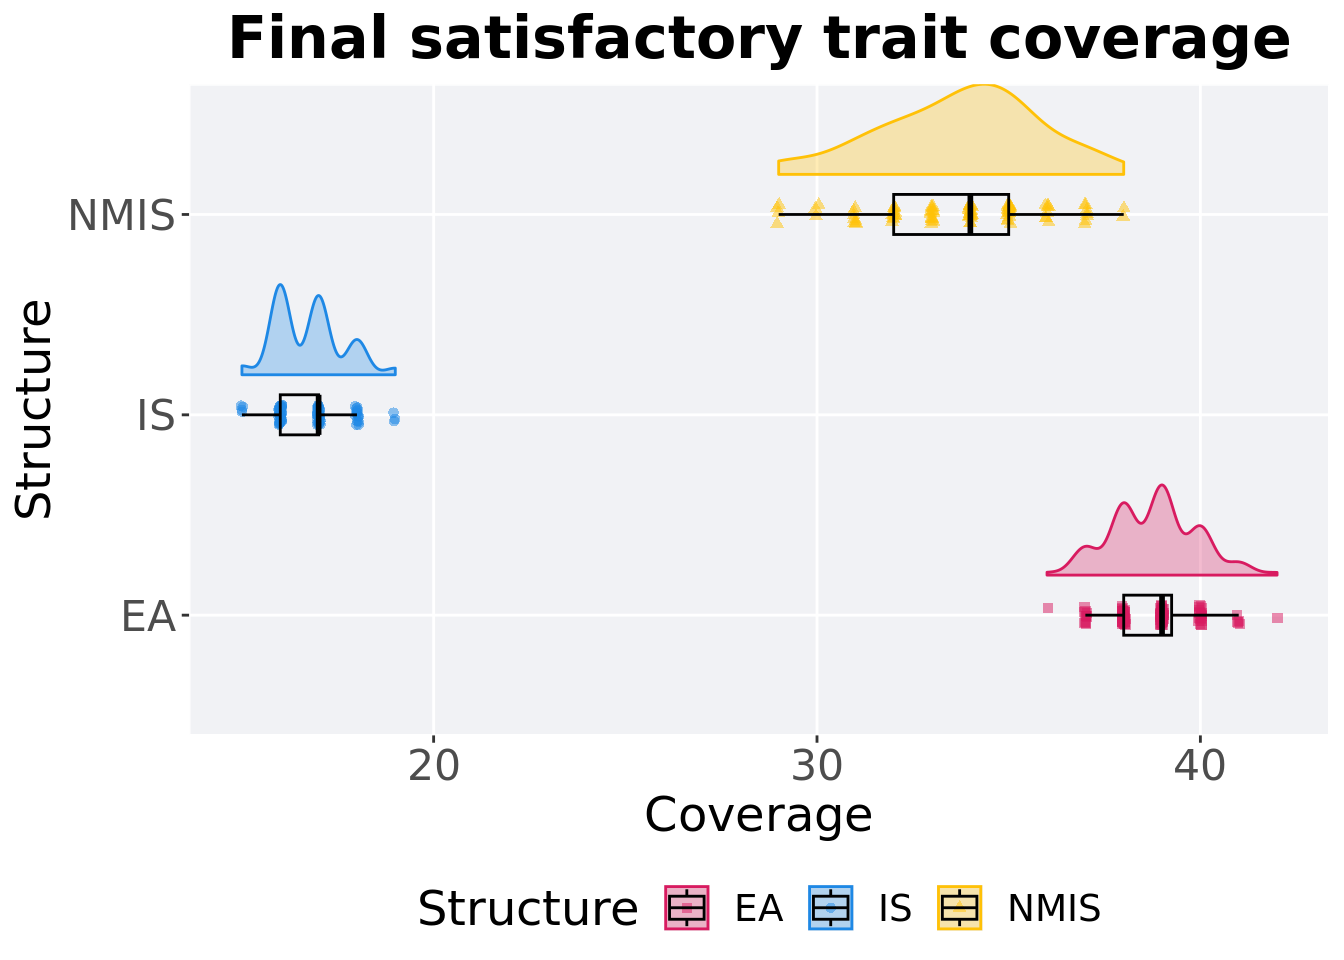
\includegraphics{demo_files/figure-latex/con-sat-lex-end-1.pdf}

\hypertarget{stats-15}{%
\paragraph{Stats}\label{stats-15}}

Summary statistics for satisfactory trait coverage in the population at the end of 50,000 generations.

\begin{Shaded}
\begin{Highlighting}[]
\CommentTok{### end of run}
\NormalTok{coverage =}\StringTok{ }\KeywordTok{filter}\NormalTok{(base_over_time, Diagnostic }\OperatorTok{==}\StringTok{ 'CONTRADICTORY_OBJECTIVES'} \OperatorTok{&}\StringTok{ `}\DataTypeTok{Selection}\CharTok{\textbackslash{}n}\DataTypeTok{Scheme}\StringTok{`} \OperatorTok{==}\StringTok{ 'LEXICASE'} \OperatorTok{&}\StringTok{ }\NormalTok{Generations }\OperatorTok{==}\StringTok{ }\DecValTok{50000}\NormalTok{)}
\NormalTok{coverage}\OperatorTok{$}\NormalTok{Structure =}\StringTok{ }\KeywordTok{factor}\NormalTok{(coverage}\OperatorTok{$}\NormalTok{Structure, }\DataTypeTok{levels=}\KeywordTok{c}\NormalTok{(}\StringTok{'EA'}\NormalTok{,}\StringTok{'NMIS'}\NormalTok{,}\StringTok{'IS'}\NormalTok{))}
\NormalTok{coverage }\OperatorTok
\StringTok{  }\KeywordTok{group_by}\NormalTok{(Structure) }\OperatorTok
\StringTok{  }\NormalTok{dplyr}\OperatorTok{::}\KeywordTok{summarise}\NormalTok{(}
    \DataTypeTok{count =} \KeywordTok{n}\NormalTok{(),}
    \DataTypeTok{na_cnt =} \KeywordTok{sum}\NormalTok{(}\KeywordTok{is.na}\NormalTok{(pop_sat_cov)),}
    \DataTypeTok{min =} \KeywordTok{min}\NormalTok{(pop_sat_cov, }\DataTypeTok{na.rm =} \OtherTok{TRUE}\NormalTok{),}
    \DataTypeTok{median =} \KeywordTok{median}\NormalTok{(pop_sat_cov, }\DataTypeTok{na.rm =} \OtherTok{TRUE}\NormalTok{),}
    \DataTypeTok{mean =} \KeywordTok{mean}\NormalTok{(pop_sat_cov, }\DataTypeTok{na.rm =} \OtherTok{TRUE}\NormalTok{),}
    \DataTypeTok{max =} \KeywordTok{max}\NormalTok{(pop_sat_cov, }\DataTypeTok{na.rm =} \OtherTok{TRUE}\NormalTok{),}
    \DataTypeTok{IQR =} \KeywordTok{IQR}\NormalTok{(pop_sat_cov, }\DataTypeTok{na.rm =} \OtherTok{TRUE}\NormalTok{)}
\NormalTok{  )}
\end{Highlighting}
\end{Shaded}

\begin{verbatim}
## # A tibble: 3 x 8
##   Structure count na_cnt   min median  mean   max   IQR
##   <fct>     <int>  <int> <int>  <dbl> <dbl> <int> <dbl>
## 1 EA          100      0    36     39  38.8    42  1.25
## 2 NMIS        100      0    29     34  33.7    38  3   
## 3 IS          100      0    15     17  16.7    19  1
\end{verbatim}

Kruskal--Wallis test provides evidence of difference among satisfactory trait coverage in the population at the end of 50,000 generations.

\begin{Shaded}
\begin{Highlighting}[]
\KeywordTok{kruskal.test}\NormalTok{(pop_sat_cov }\OperatorTok{~}\StringTok{ }\NormalTok{Structure, }\DataTypeTok{data =}\NormalTok{ coverage)}
\end{Highlighting}
\end{Shaded}

\begin{verbatim}
## 
##  Kruskal-Wallis rank sum test
## 
## data:  pop_sat_cov by Structure
## Kruskal-Wallis chi-squared = 265.34, df = 2, p-value < 2.2e-16
\end{verbatim}

Results for post-hoc Wilcoxon rank-sum test with a Bonferroni correction on satisfactory trait coverage in the population at the end of 50,000 generations.

\begin{Shaded}
\begin{Highlighting}[]
\KeywordTok{pairwise.wilcox.test}\NormalTok{(}\DataTypeTok{x =}\NormalTok{ coverage}\OperatorTok{$}\NormalTok{pop_sat_cov, }\DataTypeTok{g =}\NormalTok{ coverage}\OperatorTok{$}\NormalTok{Structure, }\DataTypeTok{p.adjust.method =} \StringTok{"bonferroni"}\NormalTok{,}
                     \DataTypeTok{paired =} \OtherTok{FALSE}\NormalTok{, }\DataTypeTok{conf.int =} \OtherTok{FALSE}\NormalTok{, }\DataTypeTok{alternative =} \StringTok{'l'}\NormalTok{)}
\end{Highlighting}
\end{Shaded}

\begin{verbatim}
## 
##  Pairwise comparisons using Wilcoxon rank sum test with continuity correction 
## 
## data:  coverage$pop_sat_cov and coverage$Structure 
## 
##      EA     NMIS  
## NMIS <2e-16 -     
## IS   <2e-16 <2e-16
## 
## P value adjustment method: bonferroni
\end{verbatim}

\hypertarget{activation-gene-coverage-2}{%
\subsection{Activation gene coverage}\label{activation-gene-coverage-2}}

Activation gene coverage analysis.

\hypertarget{coverage-over-time-5}{%
\subsubsection{Coverage over time}\label{coverage-over-time-5}}

Activation gene coverage over time.

\begin{Shaded}
\begin{Highlighting}[]
\CommentTok{# data for lines and shading on plots}
\NormalTok{lines =}\StringTok{ }\KeywordTok{filter}\NormalTok{(base_over_time, Diagnostic }\OperatorTok{==}\StringTok{ 'CONTRADICTORY_OBJECTIVES'} \OperatorTok{&}\StringTok{ `}\DataTypeTok{Selection}\CharTok{\textbackslash{}n}\DataTypeTok{Scheme}\StringTok{`} \OperatorTok{==}\StringTok{ 'LEXICASE'}\NormalTok{) }\OperatorTok
\StringTok{  }\KeywordTok{group_by}\NormalTok{(Structure, Generations) }\OperatorTok
\StringTok{  }\NormalTok{dplyr}\OperatorTok{::}\KeywordTok{summarise}\NormalTok{(}
    \DataTypeTok{min =} \KeywordTok{min}\NormalTok{(pop_act_cov),}
    \DataTypeTok{mean =} \KeywordTok{mean}\NormalTok{(pop_act_cov),}
    \DataTypeTok{max =} \KeywordTok{max}\NormalTok{(pop_act_cov)}
\NormalTok{  )}
\end{Highlighting}
\end{Shaded}

\begin{verbatim}
## `summarise()` has grouped output by 'Structure'. You can override using the
## `.groups` argument.
\end{verbatim}

\begin{Shaded}
\begin{Highlighting}[]
\KeywordTok{ggplot}\NormalTok{(lines, }\KeywordTok{aes}\NormalTok{(}\DataTypeTok{x=}\NormalTok{Generations, }\DataTypeTok{y=}\NormalTok{mean, }\DataTypeTok{group =}\NormalTok{ Structure, }\DataTypeTok{fill =}\NormalTok{ Structure, }\DataTypeTok{color =}\NormalTok{ Structure, }\DataTypeTok{shape =}\NormalTok{ Structure)) }\OperatorTok{+}
\StringTok{  }\KeywordTok{geom_ribbon}\NormalTok{(}\KeywordTok{aes}\NormalTok{(}\DataTypeTok{ymin =}\NormalTok{ min, }\DataTypeTok{ymax =}\NormalTok{ max), }\DataTypeTok{alpha =} \FloatTok{0.1}\NormalTok{) }\OperatorTok{+}
\StringTok{  }\KeywordTok{geom_line}\NormalTok{(}\DataTypeTok{size =} \FloatTok{0.5}\NormalTok{) }\OperatorTok{+}
\StringTok{  }\KeywordTok{geom_point}\NormalTok{(}\DataTypeTok{data =} \KeywordTok{filter}\NormalTok{(lines, Generations }\OperatorTok\StringTok{ }\DecValTok{2000} \OperatorTok{==}\StringTok{ }\DecValTok{0}\NormalTok{), }\DataTypeTok{size =} \FloatTok{1.5}\NormalTok{, }\DataTypeTok{stroke =} \FloatTok{2.0}\NormalTok{, }\DataTypeTok{alpha =} \FloatTok{1.0}\NormalTok{) }\OperatorTok{+}
\StringTok{  }\KeywordTok{scale_y_continuous}\NormalTok{(}
    \DataTypeTok{name=}\StringTok{"Coverage"}
\NormalTok{  ) }\OperatorTok{+}
\StringTok{  }\KeywordTok{scale_x_continuous}\NormalTok{(}
    \DataTypeTok{name=}\StringTok{"Generations"}\NormalTok{,}
    \DataTypeTok{limits=}\KeywordTok{c}\NormalTok{(}\DecValTok{0}\NormalTok{, }\DecValTok{50000}\NormalTok{),}
    \DataTypeTok{breaks=}\KeywordTok{c}\NormalTok{(}\DecValTok{0}\NormalTok{, }\DecValTok{10000}\NormalTok{, }\DecValTok{20000}\NormalTok{, }\DecValTok{30000}\NormalTok{, }\DecValTok{40000}\NormalTok{, }\DecValTok{50000}\NormalTok{),}
    \DataTypeTok{labels=}\KeywordTok{c}\NormalTok{(}\StringTok{"0e+4"}\NormalTok{, }\StringTok{"1e+4"}\NormalTok{, }\StringTok{"2e+4"}\NormalTok{, }\StringTok{"3e+4"}\NormalTok{, }\StringTok{"4e+4"}\NormalTok{, }\StringTok{"5e+4"}\NormalTok{)}

\NormalTok{  ) }\OperatorTok{+}
\StringTok{  }\KeywordTok{scale_shape_manual}\NormalTok{(}\DataTypeTok{values=}\NormalTok{SHAPE)}\OperatorTok{+}
\StringTok{  }\KeywordTok{scale_colour_manual}\NormalTok{(}\DataTypeTok{values =}\NormalTok{ cb_palette) }\OperatorTok{+}
\StringTok{  }\KeywordTok{scale_fill_manual}\NormalTok{(}\DataTypeTok{values =}\NormalTok{ cb_palette) }\OperatorTok{+}
\StringTok{  }\KeywordTok{ggtitle}\NormalTok{(}\StringTok{'Activation gene coverage over time'}\NormalTok{)}\OperatorTok{+}
\StringTok{  }\NormalTok{p_theme}
\end{Highlighting}
\end{Shaded}

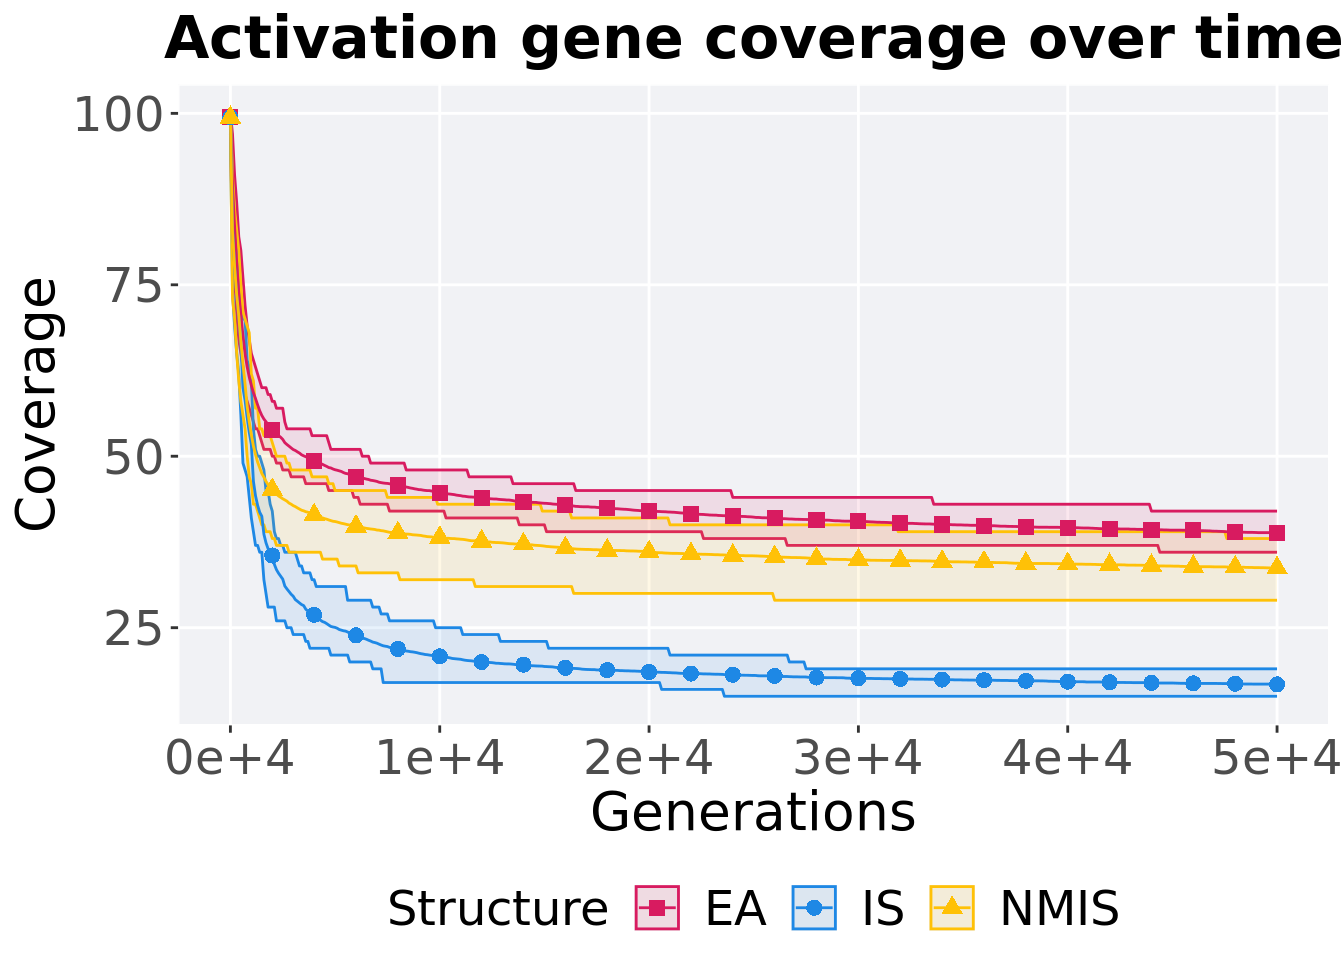
\includegraphics{demo_files/figure-latex/con-act-lex-ot-1.pdf}

\hypertarget{end-of-50000-generations-5}{%
\subsubsection{End of 50,000 generations}\label{end-of-50000-generations-5}}

Activation gene coverage in the population at the end of 50,000 generations.

\begin{Shaded}
\begin{Highlighting}[]
\CommentTok{### end of run}
\KeywordTok{filter}\NormalTok{(base_over_time, Diagnostic }\OperatorTok{==}\StringTok{ 'CONTRADICTORY_OBJECTIVES'} \OperatorTok{&}\StringTok{ `}\DataTypeTok{Selection}\CharTok{\textbackslash{}n}\DataTypeTok{Scheme}\StringTok{`} \OperatorTok{==}\StringTok{ 'LEXICASE'} \OperatorTok{&}\StringTok{ }\NormalTok{Generations }\OperatorTok{==}\StringTok{ }\DecValTok{50000}\NormalTok{) }\OperatorTok
\StringTok{  }\KeywordTok{ggplot}\NormalTok{(., }\KeywordTok{aes}\NormalTok{(}\DataTypeTok{x =}\NormalTok{ Structure, }\DataTypeTok{y =}\NormalTok{ pop_act_cov, }\DataTypeTok{color =}\NormalTok{ Structure, }\DataTypeTok{fill =}\NormalTok{ Structure, }\DataTypeTok{shape =}\NormalTok{ Structure)) }\OperatorTok{+}
\StringTok{  }\KeywordTok{geom_flat_violin}\NormalTok{(}\DataTypeTok{position =} \KeywordTok{position_nudge}\NormalTok{(}\DataTypeTok{x =} \FloatTok{.2}\NormalTok{, }\DataTypeTok{y =} \DecValTok{0}\NormalTok{), }\DataTypeTok{scale =} \StringTok{'width'}\NormalTok{, }\DataTypeTok{alpha =} \FloatTok{0.3}\NormalTok{) }\OperatorTok{+}
\StringTok{  }\KeywordTok{geom_point}\NormalTok{(}\DataTypeTok{position =} \KeywordTok{position_jitter}\NormalTok{(}\DataTypeTok{height =} \FloatTok{.05}\NormalTok{, }\DataTypeTok{width =} \FloatTok{.05}\NormalTok{), }\DataTypeTok{size =} \FloatTok{1.5}\NormalTok{, }\DataTypeTok{alpha =} \FloatTok{0.5}\NormalTok{) }\OperatorTok{+}
\StringTok{  }\KeywordTok{geom_boxplot}\NormalTok{(}\DataTypeTok{color =} \StringTok{'black'}\NormalTok{, }\DataTypeTok{width =} \FloatTok{.2}\NormalTok{, }\DataTypeTok{outlier.shape =} \OtherTok{NA}\NormalTok{, }\DataTypeTok{alpha =} \FloatTok{0.0}\NormalTok{) }\OperatorTok{+}
\StringTok{  }\KeywordTok{scale_shape_manual}\NormalTok{(}\DataTypeTok{values=}\NormalTok{SHAPE)}\OperatorTok{+}
\StringTok{  }\KeywordTok{scale_y_continuous}\NormalTok{(}
    \DataTypeTok{name=}\StringTok{"Coverage"}
\NormalTok{  ) }\OperatorTok{+}
\StringTok{  }\KeywordTok{scale_x_discrete}\NormalTok{(}
    \DataTypeTok{name=}\StringTok{"Structure"}
\NormalTok{  ) }\OperatorTok{+}
\StringTok{  }\KeywordTok{scale_colour_manual}\NormalTok{(}\DataTypeTok{values =}\NormalTok{ cb_palette) }\OperatorTok{+}
\StringTok{  }\KeywordTok{scale_fill_manual}\NormalTok{(}\DataTypeTok{values =}\NormalTok{ cb_palette) }\OperatorTok{+}
\StringTok{  }\KeywordTok{ggtitle}\NormalTok{(}\StringTok{'Final activation gene coverage'}\NormalTok{)}\OperatorTok{+}
\StringTok{  }\NormalTok{p_theme }\OperatorTok{+}\StringTok{ }\KeywordTok{coord_flip}\NormalTok{()}
\end{Highlighting}
\end{Shaded}

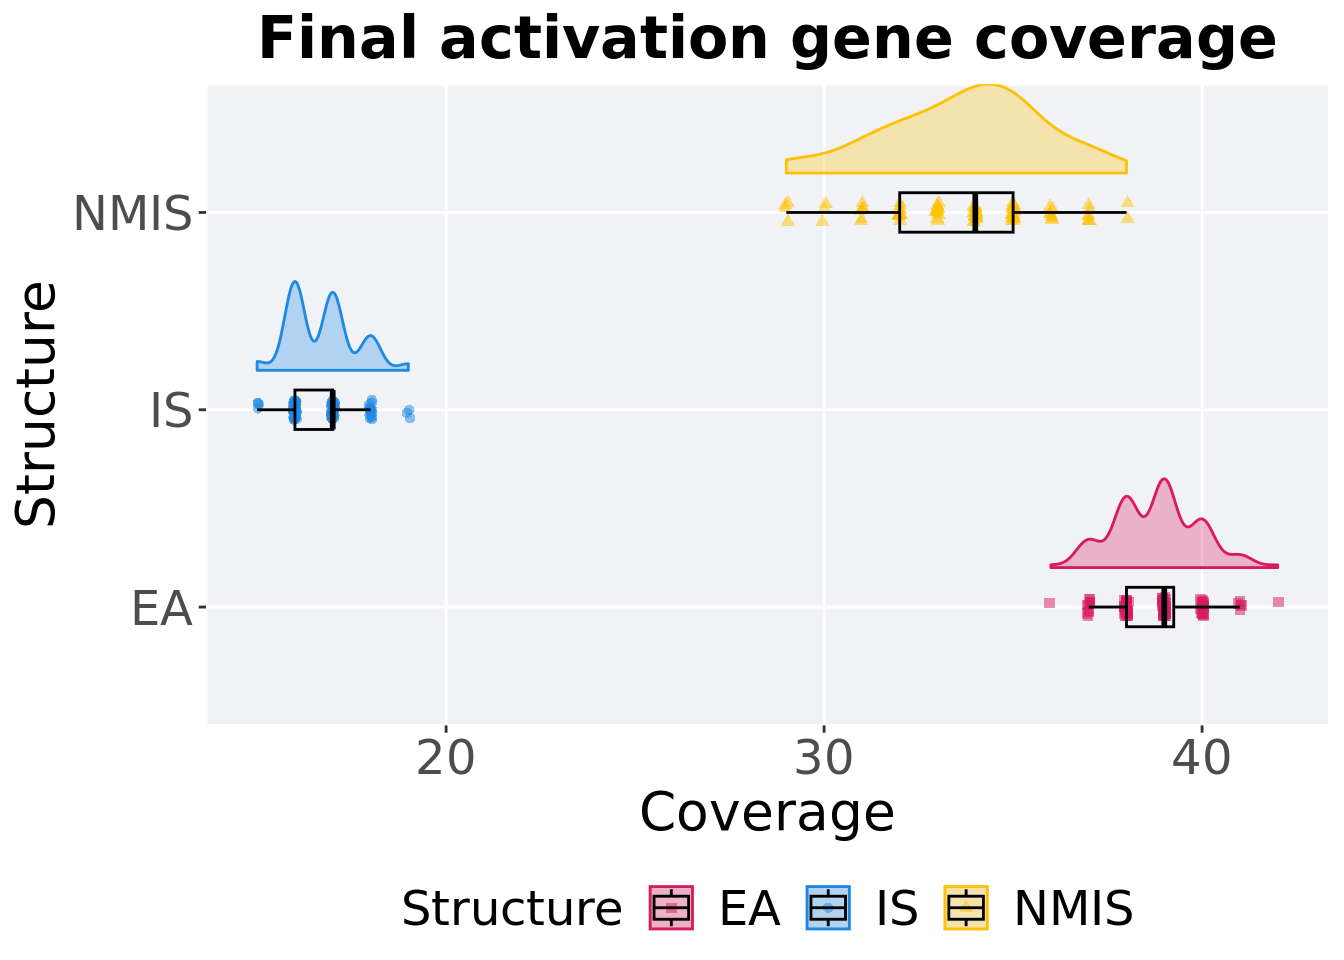
\includegraphics{demo_files/figure-latex/con-act-lex-end-1.pdf}

\hypertarget{stats-16}{%
\paragraph{Stats}\label{stats-16}}

Summary statistics for activation gene coverage.

\begin{Shaded}
\begin{Highlighting}[]
\NormalTok{coverage =}\StringTok{ }\KeywordTok{filter}\NormalTok{(base_over_time, Diagnostic }\OperatorTok{==}\StringTok{ 'CONTRADICTORY_OBJECTIVES'} \OperatorTok{&}\StringTok{ `}\DataTypeTok{Selection}\CharTok{\textbackslash{}n}\DataTypeTok{Scheme}\StringTok{`} \OperatorTok{==}\StringTok{ 'LEXICASE'} \OperatorTok{&}\StringTok{ }\NormalTok{Generations }\OperatorTok{==}\StringTok{ }\DecValTok{50000}\NormalTok{)}
\NormalTok{coverage}\OperatorTok{$}\NormalTok{Structure =}\StringTok{ }\KeywordTok{factor}\NormalTok{(coverage}\OperatorTok{$}\NormalTok{Structure, }\DataTypeTok{levels=}\KeywordTok{c}\NormalTok{(}\StringTok{'EA'}\NormalTok{,}\StringTok{'NMIS'}\NormalTok{,}\StringTok{'IS'}\NormalTok{))}
\NormalTok{coverage }\OperatorTok
\StringTok{  }\KeywordTok{group_by}\NormalTok{(Structure) }\OperatorTok
\StringTok{  }\NormalTok{dplyr}\OperatorTok{::}\KeywordTok{summarise}\NormalTok{(}
    \DataTypeTok{count =} \KeywordTok{n}\NormalTok{(),}
    \DataTypeTok{na_cnt =} \KeywordTok{sum}\NormalTok{(}\KeywordTok{is.na}\NormalTok{(pop_act_cov)),}
    \DataTypeTok{min =} \KeywordTok{min}\NormalTok{(pop_act_cov, }\DataTypeTok{na.rm =} \OtherTok{TRUE}\NormalTok{),}
    \DataTypeTok{median =} \KeywordTok{median}\NormalTok{(pop_act_cov, }\DataTypeTok{na.rm =} \OtherTok{TRUE}\NormalTok{),}
    \DataTypeTok{mean =} \KeywordTok{mean}\NormalTok{(pop_act_cov, }\DataTypeTok{na.rm =} \OtherTok{TRUE}\NormalTok{),}
    \DataTypeTok{max =} \KeywordTok{max}\NormalTok{(pop_act_cov, }\DataTypeTok{na.rm =} \OtherTok{TRUE}\NormalTok{),}
    \DataTypeTok{IQR =} \KeywordTok{IQR}\NormalTok{(pop_act_cov, }\DataTypeTok{na.rm =} \OtherTok{TRUE}\NormalTok{)}
\NormalTok{  )}
\end{Highlighting}
\end{Shaded}

\begin{verbatim}
## # A tibble: 3 x 8
##   Structure count na_cnt   min median  mean   max   IQR
##   <fct>     <int>  <int> <int>  <dbl> <dbl> <int> <dbl>
## 1 EA          100      0    36     39  38.8    42  1.25
## 2 NMIS        100      0    29     34  33.7    38  3   
## 3 IS          100      0    15     17  16.7    19  1
\end{verbatim}

Kruskal--Wallis test provides evidence of difference among activation gene coverage.

\begin{Shaded}
\begin{Highlighting}[]
\KeywordTok{kruskal.test}\NormalTok{(pop_act_cov }\OperatorTok{~}\StringTok{ }\NormalTok{Structure, }\DataTypeTok{data =}\NormalTok{ coverage)}
\end{Highlighting}
\end{Shaded}

\begin{verbatim}
## 
##  Kruskal-Wallis rank sum test
## 
## data:  pop_act_cov by Structure
## Kruskal-Wallis chi-squared = 265.34, df = 2, p-value < 2.2e-16
\end{verbatim}

Results for post-hoc Wilcoxon rank-sum test with a Bonferroni correction on activation gene coverage.

\begin{Shaded}
\begin{Highlighting}[]
\KeywordTok{pairwise.wilcox.test}\NormalTok{(}\DataTypeTok{x =}\NormalTok{ coverage}\OperatorTok{$}\NormalTok{pop_act_cov, }\DataTypeTok{g =}\NormalTok{ coverage}\OperatorTok{$}\NormalTok{Structure, }\DataTypeTok{p.adjust.method =} \StringTok{"bonferroni"}\NormalTok{,}
                     \DataTypeTok{paired =} \OtherTok{FALSE}\NormalTok{, }\DataTypeTok{conf.int =} \OtherTok{FALSE}\NormalTok{, }\DataTypeTok{alternative =} \StringTok{'l'}\NormalTok{)}
\end{Highlighting}
\end{Shaded}

\begin{verbatim}
## 
##  Pairwise comparisons using Wilcoxon rank sum test with continuity correction 
## 
## data:  coverage$pop_act_cov and coverage$Structure 
## 
##      EA     NMIS  
## NMIS <2e-16 -     
## IS   <2e-16 <2e-16
## 
## P value adjustment method: bonferroni
\end{verbatim}

\hypertarget{multi-path-exploration-results}{%
\chapter{Multi-path exploration results}\label{multi-path-exploration-results}}

Here we present the results for the \textbf{best performances} and \textbf{activation gene coverage} generated by each selection scheme replicate on the multi-path exploration diagnostic.
Best performance found refers to the largest average trait score found in a given population.
Note that activation gene coverage values are gathered at the population-level.
Activation gene coverage refers to the count of unique activation genes in a given population; this gives us a range of integers between 0 and 100.

\hypertarget{analysis-dependencies-3}{%
\section{Analysis dependencies}\label{analysis-dependencies-3}}

\begin{Shaded}
\begin{Highlighting}[]
\KeywordTok{library}\NormalTok{(ggplot2)}
\KeywordTok{library}\NormalTok{(cowplot)}
\KeywordTok{library}\NormalTok{(dplyr)}
\KeywordTok{library}\NormalTok{(PupillometryR)}
\end{Highlighting}
\end{Shaded}

\hypertarget{truncation-selection-3}{%
\section{Truncation selection}\label{truncation-selection-3}}

Here we analyze how the different population structures affect truncation selection (size 8) on the contradictory objectives diagnostic.

\hypertarget{performance}{%
\subsection{Performance}\label{performance}}

\hypertarget{performance-over-time-6}{%
\subsubsection{Performance over time}\label{performance-over-time-6}}

\begin{Shaded}
\begin{Highlighting}[]
\NormalTok{lines =}\StringTok{ }\KeywordTok{filter}\NormalTok{(base_over_time, Diagnostic }\OperatorTok{==}\StringTok{ 'MULTIPATH_EXPLORATION'} \OperatorTok{&}\StringTok{ `}\DataTypeTok{Selection}\CharTok{\textbackslash{}n}\DataTypeTok{Scheme}\StringTok{`} \OperatorTok{==}\StringTok{ 'TRUNCATION'}\NormalTok{) }\OperatorTok
\StringTok{  }\KeywordTok{group_by}\NormalTok{(Structure, Generations) }\OperatorTok
\StringTok{  }\NormalTok{dplyr}\OperatorTok{::}\KeywordTok{summarise}\NormalTok{(}
    \DataTypeTok{min =} \KeywordTok{min}\NormalTok{(pop_fit_max) }\OperatorTok{/}\StringTok{ }\NormalTok{DIMENSIONALITY,}
    \DataTypeTok{mean =} \KeywordTok{mean}\NormalTok{(pop_fit_max) }\OperatorTok{/}\StringTok{ }\NormalTok{DIMENSIONALITY,}
    \DataTypeTok{max =} \KeywordTok{max}\NormalTok{(pop_fit_max) }\OperatorTok{/}\StringTok{ }\NormalTok{DIMENSIONALITY}
\NormalTok{  )}
\KeywordTok{ggplot}\NormalTok{(lines, }\KeywordTok{aes}\NormalTok{(}\DataTypeTok{x=}\NormalTok{Generations, }\DataTypeTok{y=}\NormalTok{mean, }\DataTypeTok{group =}\NormalTok{ Structure, }\DataTypeTok{fill =}\NormalTok{ Structure, }\DataTypeTok{color =}\NormalTok{ Structure, }\DataTypeTok{shape =}\NormalTok{ Structure)) }\OperatorTok{+}
\StringTok{  }\KeywordTok{geom_ribbon}\NormalTok{(}\KeywordTok{aes}\NormalTok{(}\DataTypeTok{ymin =}\NormalTok{ min, }\DataTypeTok{ymax =}\NormalTok{ max), }\DataTypeTok{alpha =} \FloatTok{0.1}\NormalTok{) }\OperatorTok{+}
\StringTok{  }\KeywordTok{geom_line}\NormalTok{(}\DataTypeTok{size =} \FloatTok{0.5}\NormalTok{) }\OperatorTok{+}
\StringTok{  }\KeywordTok{geom_point}\NormalTok{(}\DataTypeTok{data =} \KeywordTok{filter}\NormalTok{(lines, Generations }\OperatorTok\StringTok{ }\DecValTok{2000} \OperatorTok{==}\StringTok{ }\DecValTok{0}\NormalTok{), }\DataTypeTok{size =} \FloatTok{2.5}\NormalTok{, }\DataTypeTok{stroke =} \FloatTok{2.0}\NormalTok{, }\DataTypeTok{alpha =} \FloatTok{1.0}\NormalTok{) }\OperatorTok{+}
\StringTok{  }\KeywordTok{scale_y_continuous}\NormalTok{(}
    \DataTypeTok{name=}\StringTok{"Average trait score"}
\NormalTok{  ) }\OperatorTok{+}
\StringTok{  }\KeywordTok{scale_x_continuous}\NormalTok{(}
    \DataTypeTok{name=}\StringTok{"Generations"}\NormalTok{,}
    \DataTypeTok{limits=}\KeywordTok{c}\NormalTok{(}\DecValTok{0}\NormalTok{, }\DecValTok{50000}\NormalTok{),}
    \DataTypeTok{breaks=}\KeywordTok{c}\NormalTok{(}\DecValTok{0}\NormalTok{, }\DecValTok{10000}\NormalTok{, }\DecValTok{20000}\NormalTok{, }\DecValTok{30000}\NormalTok{, }\DecValTok{40000}\NormalTok{, }\DecValTok{50000}\NormalTok{),}
    \DataTypeTok{labels=}\KeywordTok{c}\NormalTok{(}\StringTok{"0e+4"}\NormalTok{, }\StringTok{"1e+4"}\NormalTok{, }\StringTok{"2e+4"}\NormalTok{, }\StringTok{"3e+4"}\NormalTok{, }\StringTok{"4e+4"}\NormalTok{, }\StringTok{"5e+4"}\NormalTok{)}

\NormalTok{  ) }\OperatorTok{+}
\StringTok{  }\KeywordTok{scale_shape_manual}\NormalTok{(}\DataTypeTok{values=}\NormalTok{SHAPE)}\OperatorTok{+}
\StringTok{  }\KeywordTok{scale_colour_manual}\NormalTok{(}\DataTypeTok{values =}\NormalTok{ cb_palette) }\OperatorTok{+}
\StringTok{  }\KeywordTok{scale_fill_manual}\NormalTok{(}\DataTypeTok{values =}\NormalTok{ cb_palette) }\OperatorTok{+}
\StringTok{  }\KeywordTok{ggtitle}\NormalTok{(}\StringTok{"Performance over time"}\NormalTok{) }\OperatorTok{+}
\StringTok{  }\NormalTok{p_theme}
\end{Highlighting}
\end{Shaded}

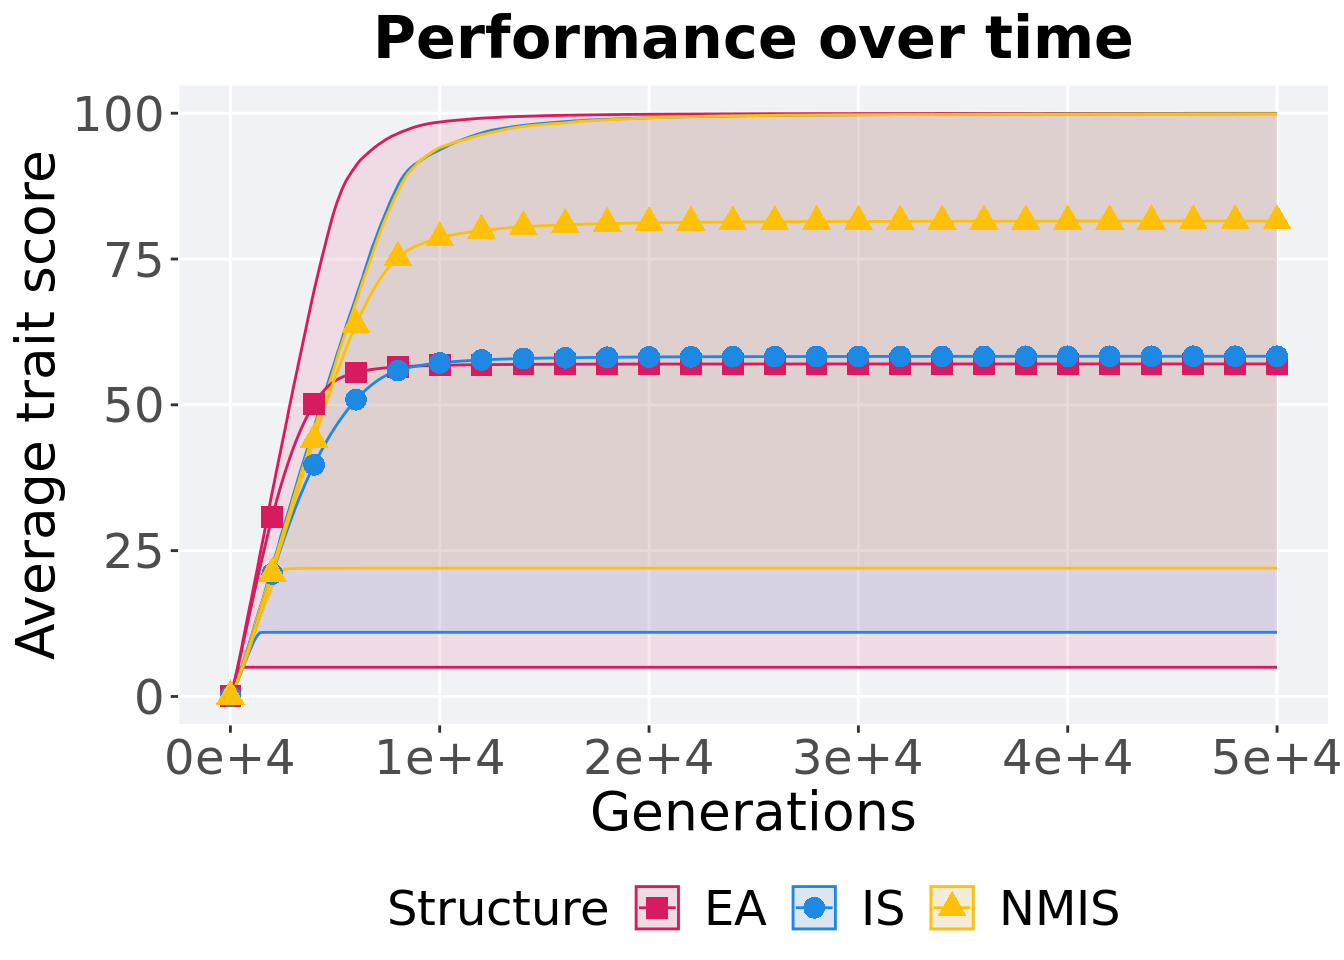
\includegraphics{demo_files/figure-latex/base-tru-mpe-perf-1.pdf}

\hypertarget{best-performance-1}{%
\subsubsection{Best performance}\label{best-performance-1}}

First generation a satisfactory solution is found throughout the 50,000 generations.

\begin{Shaded}
\begin{Highlighting}[]
\KeywordTok{filter}\NormalTok{(base_best, Diagnostic }\OperatorTok{==}\StringTok{ 'MULTIPATH_EXPLORATION'} \OperatorTok{&}\StringTok{ `}\DataTypeTok{Selection}\CharTok{\textbackslash{}n}\DataTypeTok{Scheme}\StringTok{`} \OperatorTok{==}\StringTok{ 'TRUNCATION'} \OperatorTok{&}\StringTok{ }\NormalTok{VAR }\OperatorTok{==}\StringTok{ 'pop_fit_max'}\NormalTok{) }\OperatorTok
\StringTok{  }\KeywordTok{ggplot}\NormalTok{(., }\KeywordTok{aes}\NormalTok{(}\DataTypeTok{x =}\NormalTok{ Structure, }\DataTypeTok{y =}\NormalTok{ VAL }\OperatorTok{/}\StringTok{ }\NormalTok{DIMENSIONALITY, }\DataTypeTok{color =}\NormalTok{ Structure, }\DataTypeTok{fill =}\NormalTok{ Structure, }\DataTypeTok{shape =}\NormalTok{ Structure)) }\OperatorTok{+}
\StringTok{  }\KeywordTok{geom_flat_violin}\NormalTok{(}\DataTypeTok{position =} \KeywordTok{position_nudge}\NormalTok{(}\DataTypeTok{x =} \FloatTok{.2}\NormalTok{, }\DataTypeTok{y =} \DecValTok{0}\NormalTok{), }\DataTypeTok{scale =} \StringTok{'width'}\NormalTok{, }\DataTypeTok{alpha =} \FloatTok{0.2}\NormalTok{) }\OperatorTok{+}
\StringTok{  }\KeywordTok{geom_point}\NormalTok{(}\DataTypeTok{position =} \KeywordTok{position_jitter}\NormalTok{(}\DataTypeTok{width =} \FloatTok{.1}\NormalTok{), }\DataTypeTok{size =} \FloatTok{1.5}\NormalTok{, }\DataTypeTok{alpha =} \FloatTok{1.0}\NormalTok{) }\OperatorTok{+}
\StringTok{  }\KeywordTok{geom_boxplot}\NormalTok{(}\DataTypeTok{color =} \StringTok{'black'}\NormalTok{, }\DataTypeTok{width =} \FloatTok{.2}\NormalTok{, }\DataTypeTok{outlier.shape =} \OtherTok{NA}\NormalTok{, }\DataTypeTok{alpha =} \FloatTok{0.0}\NormalTok{) }\OperatorTok{+}
\StringTok{  }\KeywordTok{scale_y_continuous}\NormalTok{(}
    \DataTypeTok{name=}\StringTok{"Average trait score"}
\NormalTok{  ) }\OperatorTok{+}
\StringTok{  }\KeywordTok{scale_x_discrete}\NormalTok{(}
    \DataTypeTok{name=}\StringTok{"Structure"}
\NormalTok{  )}\OperatorTok{+}
\StringTok{  }\KeywordTok{scale_shape_manual}\NormalTok{(}\DataTypeTok{values=}\NormalTok{SHAPE)}\OperatorTok{+}
\StringTok{  }\KeywordTok{scale_colour_manual}\NormalTok{(}\DataTypeTok{values =}\NormalTok{ cb_palette, ) }\OperatorTok{+}
\StringTok{  }\KeywordTok{scale_fill_manual}\NormalTok{(}\DataTypeTok{values =}\NormalTok{ cb_palette) }\OperatorTok{+}
\StringTok{  }\KeywordTok{ggtitle}\NormalTok{(}\StringTok{'Best performance'}\NormalTok{)}\OperatorTok{+}
\StringTok{  }\NormalTok{p_theme }\OperatorTok{+}\StringTok{ }\KeywordTok{coord_flip}\NormalTok{()}
\end{Highlighting}
\end{Shaded}

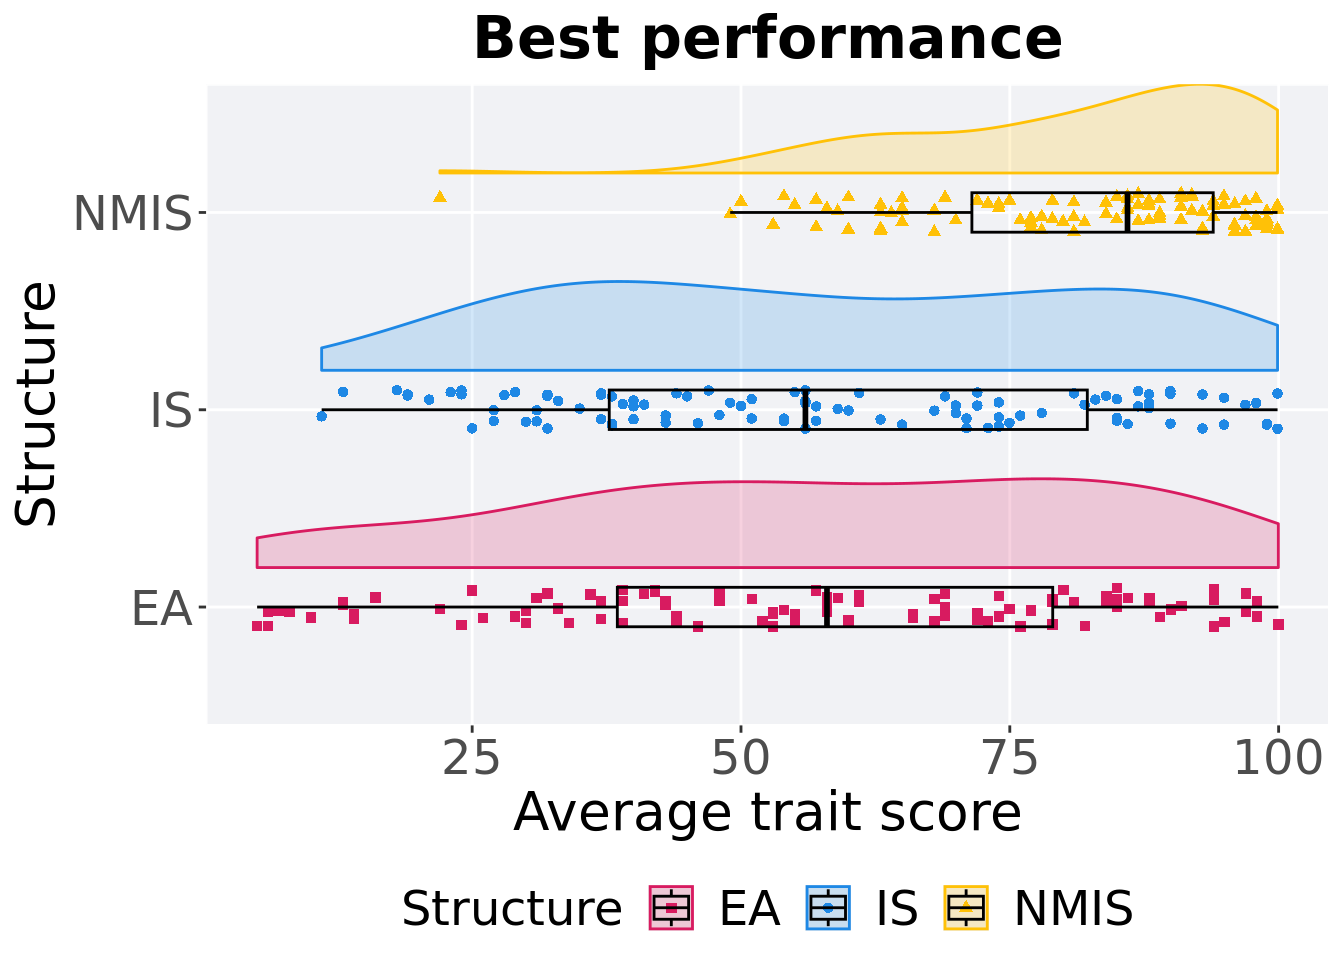
\includegraphics{demo_files/figure-latex/base-tru-mpe-per-bst-1.pdf}

\hypertarget{stats-17}{%
\paragraph{Stats}\label{stats-17}}

Summary statistics for the first generation a satisfactory solution is found.

\begin{Shaded}
\begin{Highlighting}[]
\NormalTok{performance =}\StringTok{ }\KeywordTok{filter}\NormalTok{(base_best, Diagnostic }\OperatorTok{==}\StringTok{ 'MULTIPATH_EXPLORATION'} \OperatorTok{&}\StringTok{ `}\DataTypeTok{Selection}\CharTok{\textbackslash{}n}\DataTypeTok{Scheme}\StringTok{`} \OperatorTok{==}\StringTok{ 'TRUNCATION'} \OperatorTok{&}\StringTok{ }\NormalTok{VAR }\OperatorTok{==}\StringTok{ 'pop_fit_max'}\NormalTok{)}
\NormalTok{performance }\OperatorTok
\StringTok{  }\KeywordTok{group_by}\NormalTok{(Structure) }\OperatorTok
\StringTok{  }\NormalTok{dplyr}\OperatorTok{::}\KeywordTok{summarise}\NormalTok{(}
    \DataTypeTok{count =} \KeywordTok{n}\NormalTok{(),}
    \DataTypeTok{na_cnt =} \KeywordTok{sum}\NormalTok{(}\KeywordTok{is.na}\NormalTok{(VAL)),}
    \DataTypeTok{min =} \KeywordTok{min}\NormalTok{(VAL, }\DataTypeTok{na.rm =} \OtherTok{TRUE}\NormalTok{) }\OperatorTok{/}\StringTok{ }\NormalTok{DIMENSIONALITY,}
    \DataTypeTok{median =} \KeywordTok{median}\NormalTok{(VAL, }\DataTypeTok{na.rm =} \OtherTok{TRUE}\NormalTok{) }\OperatorTok{/}\StringTok{ }\NormalTok{DIMENSIONALITY,}
    \DataTypeTok{mean =} \KeywordTok{mean}\NormalTok{(VAL, }\DataTypeTok{na.rm =} \OtherTok{TRUE}\NormalTok{) }\OperatorTok{/}\StringTok{ }\NormalTok{DIMENSIONALITY,}
    \DataTypeTok{max =} \KeywordTok{max}\NormalTok{(VAL, }\DataTypeTok{na.rm =} \OtherTok{TRUE}\NormalTok{) }\OperatorTok{/}\StringTok{ }\NormalTok{DIMENSIONALITY,}
    \DataTypeTok{IQR =} \KeywordTok{IQR}\NormalTok{(VAL, }\DataTypeTok{na.rm =} \OtherTok{TRUE}\NormalTok{) }\OperatorTok{/}\StringTok{ }\NormalTok{DIMENSIONALITY}
\NormalTok{  )}
\end{Highlighting}
\end{Shaded}

\begin{verbatim}
## # A tibble: 3 x 8
##   Structure count na_cnt   min median  mean   max   IQR
##   <fct>     <int>  <int> <dbl>  <dbl> <dbl> <dbl> <dbl>
## 1 EA          100      0   5     58.0  57.0 100.   40.5
## 2 IS          100      0  11     56.0  58.3  99.9  44.5
## 3 NMIS        100      0  22.0   85.9  81.5  99.9  22.4
\end{verbatim}

Kruskal--Wallis test provides evidence of difference among selection schemes.

\begin{Shaded}
\begin{Highlighting}[]
\KeywordTok{kruskal.test}\NormalTok{(VAL }\OperatorTok{~}\StringTok{ }\NormalTok{Structure, }\DataTypeTok{data =}\NormalTok{ performance)}
\end{Highlighting}
\end{Shaded}

\begin{verbatim}
## 
##  Kruskal-Wallis rank sum test
## 
## data:  VAL by Structure
## Kruskal-Wallis chi-squared = 57.688, df = 2, p-value = 2.973e-13
\end{verbatim}

Results for post-hoc Wilcoxon rank-sum test with a Bonferroni correction.

\begin{Shaded}
\begin{Highlighting}[]
\KeywordTok{pairwise.wilcox.test}\NormalTok{(}\DataTypeTok{x =}\NormalTok{ performance}\OperatorTok{$}\NormalTok{VAL, }\DataTypeTok{g =}\NormalTok{ performance}\OperatorTok{$}\NormalTok{Structure, }\DataTypeTok{p.adjust.method =} \StringTok{"bonferroni"}\NormalTok{,}
                     \DataTypeTok{paired =} \OtherTok{FALSE}\NormalTok{, }\DataTypeTok{conf.int =} \OtherTok{FALSE}\NormalTok{, }\DataTypeTok{alternative =} \StringTok{'g'}\NormalTok{)}
\end{Highlighting}
\end{Shaded}

\begin{verbatim}
## 
##  Pairwise comparisons using Wilcoxon rank sum test with continuity correction 
## 
## data:  performance$VAL and performance$Structure 
## 
##      EA      IS     
## IS   1       -      
## NMIS 4.3e-11 1.3e-10
## 
## P value adjustment method: bonferroni
\end{verbatim}

\hypertarget{final-performance-1}{%
\subsubsection{Final performance}\label{final-performance-1}}

First generation a satisfactory solution is found throughout the 50,000 generations.

\begin{Shaded}
\begin{Highlighting}[]
\KeywordTok{filter}\NormalTok{(base_over_time, Diagnostic }\OperatorTok{==}\StringTok{ 'MULTIPATH_EXPLORATION'} \OperatorTok{&}\StringTok{ `}\DataTypeTok{Selection}\CharTok{\textbackslash{}n}\DataTypeTok{Scheme}\StringTok{`} \OperatorTok{==}\StringTok{ 'TRUNCATION'} \OperatorTok{&}\StringTok{ }\NormalTok{Generations }\OperatorTok{==}\StringTok{ }\DecValTok{50000}\NormalTok{) }\OperatorTok
\StringTok{  }\KeywordTok{ggplot}\NormalTok{(., }\KeywordTok{aes}\NormalTok{(}\DataTypeTok{x =}\NormalTok{ Structure, }\DataTypeTok{y =}\NormalTok{ pop_fit_max }\OperatorTok{/}\StringTok{ }\NormalTok{DIMENSIONALITY, }\DataTypeTok{color =}\NormalTok{ Structure, }\DataTypeTok{fill =}\NormalTok{ Structure, }\DataTypeTok{shape =}\NormalTok{ Structure)) }\OperatorTok{+}
\StringTok{  }\KeywordTok{geom_flat_violin}\NormalTok{(}\DataTypeTok{position =} \KeywordTok{position_nudge}\NormalTok{(}\DataTypeTok{x =} \FloatTok{.2}\NormalTok{, }\DataTypeTok{y =} \DecValTok{0}\NormalTok{), }\DataTypeTok{scale =} \StringTok{'width'}\NormalTok{, }\DataTypeTok{alpha =} \FloatTok{0.2}\NormalTok{) }\OperatorTok{+}
\StringTok{  }\KeywordTok{geom_point}\NormalTok{(}\DataTypeTok{position =} \KeywordTok{position_jitter}\NormalTok{(}\DataTypeTok{width =} \FloatTok{.1}\NormalTok{), }\DataTypeTok{size =} \FloatTok{1.5}\NormalTok{, }\DataTypeTok{alpha =} \FloatTok{1.0}\NormalTok{) }\OperatorTok{+}
\StringTok{  }\KeywordTok{geom_boxplot}\NormalTok{(}\DataTypeTok{color =} \StringTok{'black'}\NormalTok{, }\DataTypeTok{width =} \FloatTok{.2}\NormalTok{, }\DataTypeTok{outlier.shape =} \OtherTok{NA}\NormalTok{, }\DataTypeTok{alpha =} \FloatTok{0.0}\NormalTok{) }\OperatorTok{+}
\StringTok{  }\KeywordTok{scale_y_continuous}\NormalTok{(}
    \DataTypeTok{name=}\StringTok{"Average trait score"}
\NormalTok{  ) }\OperatorTok{+}
\StringTok{  }\KeywordTok{scale_x_discrete}\NormalTok{(}
    \DataTypeTok{name=}\StringTok{"Structure"}
\NormalTok{  )}\OperatorTok{+}
\StringTok{  }\KeywordTok{scale_shape_manual}\NormalTok{(}\DataTypeTok{values=}\NormalTok{SHAPE)}\OperatorTok{+}
\StringTok{  }\KeywordTok{scale_colour_manual}\NormalTok{(}\DataTypeTok{values =}\NormalTok{ cb_palette, ) }\OperatorTok{+}
\StringTok{  }\KeywordTok{scale_fill_manual}\NormalTok{(}\DataTypeTok{values =}\NormalTok{ cb_palette) }\OperatorTok{+}
\StringTok{  }\KeywordTok{ggtitle}\NormalTok{(}\StringTok{'Final performance'}\NormalTok{)}\OperatorTok{+}
\StringTok{  }\NormalTok{p_theme }\OperatorTok{+}\StringTok{ }\KeywordTok{coord_flip}\NormalTok{()}
\end{Highlighting}
\end{Shaded}

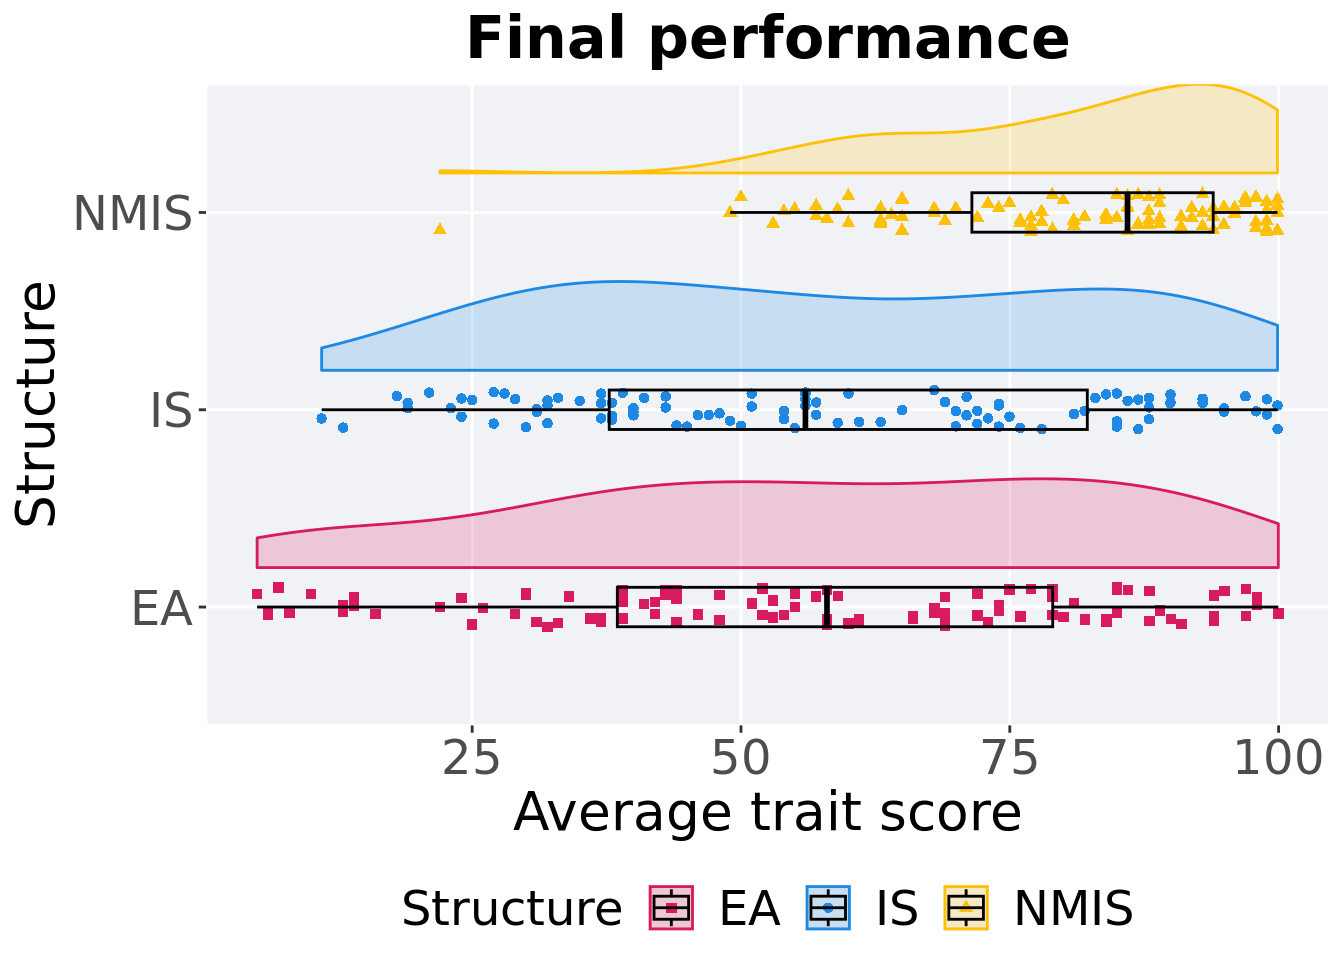
\includegraphics{demo_files/figure-latex/base-tru-mpe-per-end-1.pdf}

\hypertarget{stats-18}{%
\paragraph{Stats}\label{stats-18}}

Summary statistics for the first generation a satisfactory solution is found.

\begin{Shaded}
\begin{Highlighting}[]
\NormalTok{performance =}\StringTok{ }\KeywordTok{filter}\NormalTok{(base_over_time, Diagnostic }\OperatorTok{==}\StringTok{ 'MULTIPATH_EXPLORATION'} \OperatorTok{&}\StringTok{ `}\DataTypeTok{Selection}\CharTok{\textbackslash{}n}\DataTypeTok{Scheme}\StringTok{`} \OperatorTok{==}\StringTok{ 'TRUNCATION'} \OperatorTok{&}\StringTok{ }\NormalTok{Generations }\OperatorTok{==}\StringTok{ }\DecValTok{50000}\NormalTok{)}
\NormalTok{performance }\OperatorTok
\StringTok{  }\KeywordTok{group_by}\NormalTok{(Structure) }\OperatorTok
\StringTok{  }\NormalTok{dplyr}\OperatorTok{::}\KeywordTok{summarise}\NormalTok{(}
    \DataTypeTok{count =} \KeywordTok{n}\NormalTok{(),}
    \DataTypeTok{na_cnt =} \KeywordTok{sum}\NormalTok{(}\KeywordTok{is.na}\NormalTok{(pop_fit_max)),}
    \DataTypeTok{min =} \KeywordTok{min}\NormalTok{(pop_fit_max }\OperatorTok{/}\StringTok{ }\NormalTok{DIMENSIONALITY, }\DataTypeTok{na.rm =} \OtherTok{TRUE}\NormalTok{),}
    \DataTypeTok{median =} \KeywordTok{median}\NormalTok{(pop_fit_max }\OperatorTok{/}\StringTok{ }\NormalTok{DIMENSIONALITY, }\DataTypeTok{na.rm =} \OtherTok{TRUE}\NormalTok{),}
    \DataTypeTok{mean =} \KeywordTok{mean}\NormalTok{(pop_fit_max }\OperatorTok{/}\StringTok{ }\NormalTok{DIMENSIONALITY, }\DataTypeTok{na.rm =} \OtherTok{TRUE}\NormalTok{),}
    \DataTypeTok{max =} \KeywordTok{max}\NormalTok{(pop_fit_max }\OperatorTok{/}\StringTok{ }\NormalTok{DIMENSIONALITY, }\DataTypeTok{na.rm =} \OtherTok{TRUE}\NormalTok{),}
    \DataTypeTok{IQR =} \KeywordTok{IQR}\NormalTok{(pop_fit_max }\OperatorTok{/}\StringTok{ }\NormalTok{DIMENSIONALITY, }\DataTypeTok{na.rm =} \OtherTok{TRUE}\NormalTok{)}
\NormalTok{  )}
\end{Highlighting}
\end{Shaded}

\begin{verbatim}
## # A tibble: 3 x 8
##   Structure count na_cnt   min median  mean   max   IQR
##   <fct>     <int>  <int> <dbl>  <dbl> <dbl> <dbl> <dbl>
## 1 EA          100      0   5     58.0  57.0 100.   40.5
## 2 IS          100      0  11     56.0  58.3  99.9  44.5
## 3 NMIS        100      0  22.0   85.9  81.5  99.9  22.4
\end{verbatim}

Kruskal--Wallis test provides evidence of difference among selection schemes.

\begin{Shaded}
\begin{Highlighting}[]
\KeywordTok{kruskal.test}\NormalTok{(pop_fit_max }\OperatorTok{~}\StringTok{ }\NormalTok{Structure, }\DataTypeTok{data =}\NormalTok{ performance)}
\end{Highlighting}
\end{Shaded}

\begin{verbatim}
## 
##  Kruskal-Wallis rank sum test
## 
## data:  pop_fit_max by Structure
## Kruskal-Wallis chi-squared = 57.688, df = 2, p-value = 2.973e-13
\end{verbatim}

Results for post-hoc Wilcoxon rank-sum test with a Bonferroni correction.

\begin{Shaded}
\begin{Highlighting}[]
\KeywordTok{pairwise.wilcox.test}\NormalTok{(}\DataTypeTok{x =}\NormalTok{ performance}\OperatorTok{$}\NormalTok{pop_fit_max, }\DataTypeTok{g =}\NormalTok{ performance}\OperatorTok{$}\NormalTok{Structure, }\DataTypeTok{p.adjust.method =} \StringTok{"bonferroni"}\NormalTok{,}
                     \DataTypeTok{paired =} \OtherTok{FALSE}\NormalTok{, }\DataTypeTok{conf.int =} \OtherTok{FALSE}\NormalTok{, }\DataTypeTok{alternative =} \StringTok{'g'}\NormalTok{)}
\end{Highlighting}
\end{Shaded}

\begin{verbatim}
## 
##  Pairwise comparisons using Wilcoxon rank sum test with continuity correction 
## 
## data:  performance$pop_fit_max and performance$Structure 
## 
##      EA      IS     
## IS   1       -      
## NMIS 4.3e-11 1.3e-10
## 
## P value adjustment method: bonferroni
\end{verbatim}

\hypertarget{generation-satisfactory-solution-found-6}{%
\subsection{Generation satisfactory solution found}\label{generation-satisfactory-solution-found-6}}

First generation a satisfactory solution is found throughout the 50,000 generations.

\begin{Shaded}
\begin{Highlighting}[]
\KeywordTok{filter}\NormalTok{(base_ssf, Diagnostic }\OperatorTok{==}\StringTok{ 'MULTIPATH_EXPLORATION'} \OperatorTok{&}\StringTok{ `}\DataTypeTok{Selection}\CharTok{\textbackslash{}n}\DataTypeTok{Scheme}\StringTok{`} \OperatorTok{==}\StringTok{ 'TRUNCATION'}\OperatorTok{&}\StringTok{ }\NormalTok{Generations }\OperatorTok{<=}\StringTok{ }\NormalTok{GENERATIONS) }\OperatorTok
\StringTok{  }\KeywordTok{ggplot}\NormalTok{(., }\KeywordTok{aes}\NormalTok{(}\DataTypeTok{x =}\NormalTok{ Structure, }\DataTypeTok{y =}\NormalTok{ Generations, }\DataTypeTok{color =}\NormalTok{ Structure, }\DataTypeTok{fill =}\NormalTok{ Structure, }\DataTypeTok{shape =}\NormalTok{ Structure)) }\OperatorTok{+}
\StringTok{    }\KeywordTok{geom_flat_violin}\NormalTok{(}\DataTypeTok{position =} \KeywordTok{position_nudge}\NormalTok{(}\DataTypeTok{x =} \FloatTok{.2}\NormalTok{, }\DataTypeTok{y =} \DecValTok{0}\NormalTok{), }\DataTypeTok{scale =} \StringTok{'width'}\NormalTok{, }\DataTypeTok{alpha =} \FloatTok{0.2}\NormalTok{) }\OperatorTok{+}
\StringTok{  }\KeywordTok{geom_point}\NormalTok{(}\DataTypeTok{position =} \KeywordTok{position_jitter}\NormalTok{(}\DataTypeTok{width =} \FloatTok{.1}\NormalTok{), }\DataTypeTok{size =} \FloatTok{1.5}\NormalTok{, }\DataTypeTok{alpha =} \FloatTok{1.0}\NormalTok{) }\OperatorTok{+}
\StringTok{  }\KeywordTok{geom_boxplot}\NormalTok{(}\DataTypeTok{color =} \StringTok{'black'}\NormalTok{, }\DataTypeTok{width =} \FloatTok{.2}\NormalTok{, }\DataTypeTok{outlier.shape =} \OtherTok{NA}\NormalTok{, }\DataTypeTok{alpha =} \FloatTok{0.0}\NormalTok{) }\OperatorTok{+}
\StringTok{  }\KeywordTok{scale_shape_manual}\NormalTok{(}\DataTypeTok{values=}\NormalTok{SHAPE)}\OperatorTok{+}
\StringTok{  }\KeywordTok{scale_y_continuous}\NormalTok{(}
    \DataTypeTok{name=}\StringTok{"Generations"}
\NormalTok{  ) }\OperatorTok{+}
\StringTok{  }\KeywordTok{scale_x_discrete}\NormalTok{(}
    \DataTypeTok{name=}\StringTok{"Structure"}
\NormalTok{  ) }\OperatorTok{+}
\StringTok{  }\KeywordTok{scale_colour_manual}\NormalTok{(}\DataTypeTok{values =}\NormalTok{ cb_palette) }\OperatorTok{+}
\StringTok{  }\KeywordTok{scale_fill_manual}\NormalTok{(}\DataTypeTok{values =}\NormalTok{ cb_palette) }\OperatorTok{+}
\StringTok{  }\NormalTok{p_theme }\OperatorTok{+}\StringTok{ }\KeywordTok{coord_flip}\NormalTok{()}
\end{Highlighting}
\end{Shaded}

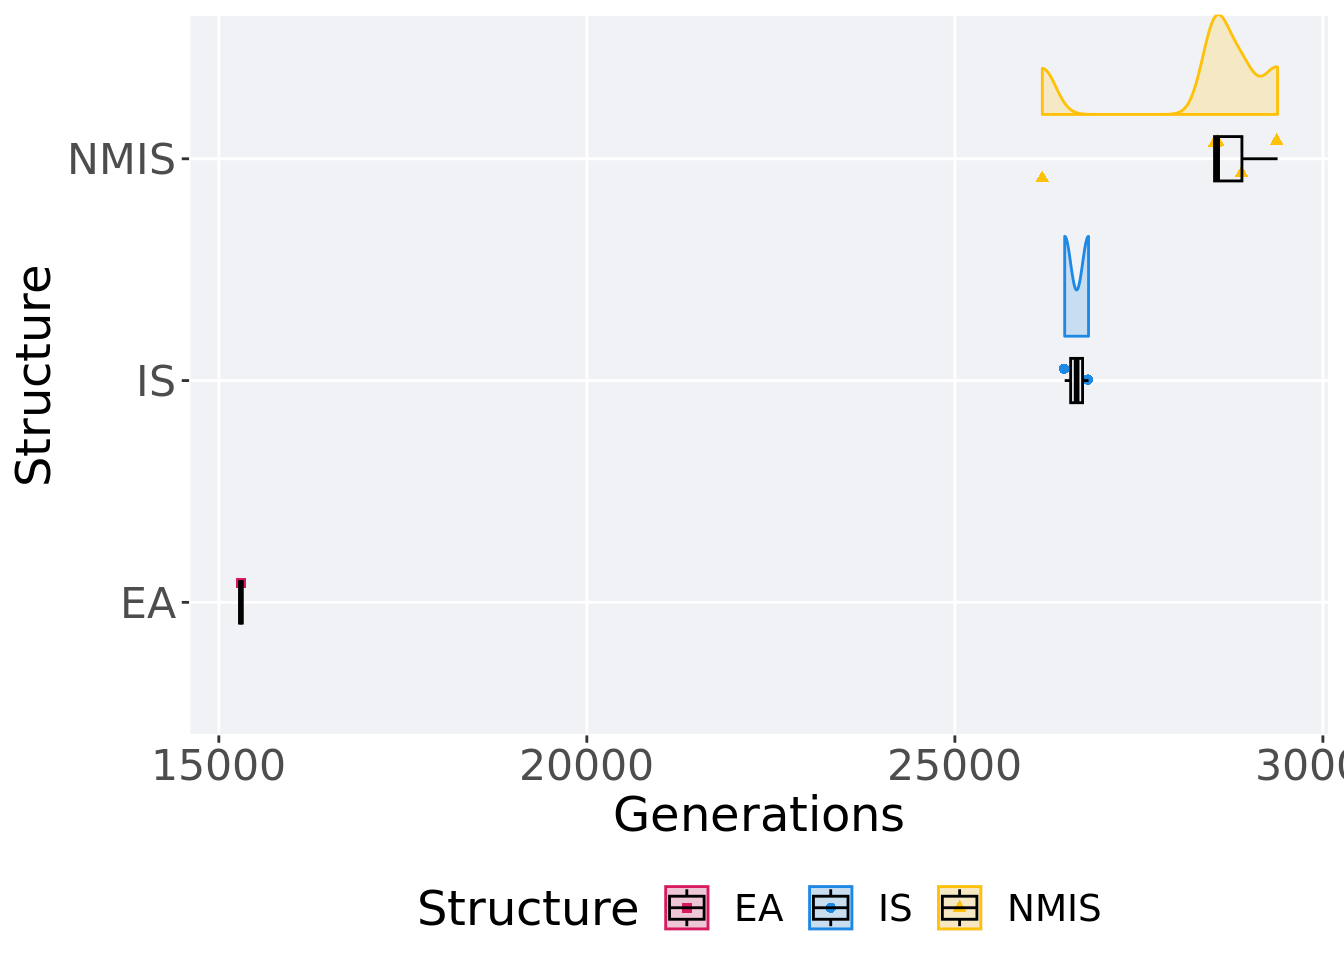
\includegraphics{demo_files/figure-latex/base-tru-mpe-ssf-1.pdf}

\hypertarget{stats-19}{%
\subsubsection{Stats}\label{stats-19}}

Summary statistics for the first generation a satisfactory solution is found.

\begin{Shaded}
\begin{Highlighting}[]
\NormalTok{ssf =}\StringTok{ }\KeywordTok{filter}\NormalTok{(base_ssf, Diagnostic }\OperatorTok{==}\StringTok{ 'MULTIPATH_EXPLORATION'} \OperatorTok{&}\StringTok{ `}\DataTypeTok{Selection}\CharTok{\textbackslash{}n}\DataTypeTok{Scheme}\StringTok{`} \OperatorTok{==}\StringTok{ 'TRUNCATION'} \OperatorTok{&}\StringTok{ }\NormalTok{Generations }\OperatorTok{<}\StringTok{ }\DecValTok{60000}\NormalTok{)}
\NormalTok{ssf }\OperatorTok
\StringTok{  }\KeywordTok{group_by}\NormalTok{(Structure) }\OperatorTok
\StringTok{  }\NormalTok{dplyr}\OperatorTok{::}\KeywordTok{summarise}\NormalTok{(}
    \DataTypeTok{count =} \KeywordTok{n}\NormalTok{(),}
    \DataTypeTok{na_cnt =} \KeywordTok{sum}\NormalTok{(}\KeywordTok{is.na}\NormalTok{(Generations)),}
    \DataTypeTok{min =} \KeywordTok{min}\NormalTok{(Generations, }\DataTypeTok{na.rm =} \OtherTok{TRUE}\NormalTok{),}
    \DataTypeTok{median =} \KeywordTok{median}\NormalTok{(Generations, }\DataTypeTok{na.rm =} \OtherTok{TRUE}\NormalTok{),}
    \DataTypeTok{mean =} \KeywordTok{mean}\NormalTok{(Generations, }\DataTypeTok{na.rm =} \OtherTok{TRUE}\NormalTok{),}
    \DataTypeTok{max =} \KeywordTok{max}\NormalTok{(Generations, }\DataTypeTok{na.rm =} \OtherTok{TRUE}\NormalTok{),}
    \DataTypeTok{IQR =} \KeywordTok{IQR}\NormalTok{(Generations, }\DataTypeTok{na.rm =} \OtherTok{TRUE}\NormalTok{)}
\NormalTok{  )}
\end{Highlighting}
\end{Shaded}

\begin{verbatim}
## # A tibble: 3 x 8
##   Structure count na_cnt   min median   mean   max   IQR
##   <fct>     <int>  <int> <int>  <dbl>  <dbl> <int> <dbl>
## 1 EA            1      0 15300  15300 15300  15300     0
## 2 IS            2      0 26492  26654 26654  26816   162
## 3 NMIS          5      0 26188  28563 28313. 29384   372
\end{verbatim}

Kruskal--Wallis test provides evidence of no difference among selection schemes.

\begin{Shaded}
\begin{Highlighting}[]
\KeywordTok{kruskal.test}\NormalTok{(Generations }\OperatorTok{~}\StringTok{ }\NormalTok{Structure, }\DataTypeTok{data =}\NormalTok{ ssf)}
\end{Highlighting}
\end{Shaded}

\begin{verbatim}
## 
##  Kruskal-Wallis rank sum test
## 
## data:  Generations by Structure
## Kruskal-Wallis chi-squared = 3.3833, df = 2, p-value = 0.1842
\end{verbatim}

\hypertarget{activation-gene-coverage-3}{%
\subsection{Activation gene coverage}\label{activation-gene-coverage-3}}

Activation gene coverage analysis.

\hypertarget{coverage-over-time-6}{%
\subsubsection{Coverage over time}\label{coverage-over-time-6}}

Activation gene coverage over time.

\begin{Shaded}
\begin{Highlighting}[]
\CommentTok{# data for lines and shading on plots}
\NormalTok{lines =}\StringTok{ }\KeywordTok{filter}\NormalTok{(base_over_time, Diagnostic }\OperatorTok{==}\StringTok{ 'MULTIPATH_EXPLORATION'} \OperatorTok{&}\StringTok{ `}\DataTypeTok{Selection}\CharTok{\textbackslash{}n}\DataTypeTok{Scheme}\StringTok{`} \OperatorTok{==}\StringTok{ 'TRUNCATION'}\NormalTok{) }\OperatorTok
\StringTok{  }\KeywordTok{group_by}\NormalTok{(Structure, Generations) }\OperatorTok
\StringTok{  }\NormalTok{dplyr}\OperatorTok{::}\KeywordTok{summarise}\NormalTok{(}
    \DataTypeTok{min =} \KeywordTok{min}\NormalTok{(pop_act_cov),}
    \DataTypeTok{mean =} \KeywordTok{mean}\NormalTok{(pop_act_cov),}
    \DataTypeTok{max =} \KeywordTok{max}\NormalTok{(pop_act_cov)}
\NormalTok{  )}
\end{Highlighting}
\end{Shaded}

\begin{verbatim}
## `summarise()` has grouped output by 'Structure'. You can override using the
## `.groups` argument.
\end{verbatim}

\begin{Shaded}
\begin{Highlighting}[]
\KeywordTok{ggplot}\NormalTok{(lines, }\KeywordTok{aes}\NormalTok{(}\DataTypeTok{x=}\NormalTok{Generations, }\DataTypeTok{y=}\NormalTok{mean, }\DataTypeTok{group =}\NormalTok{ Structure, }\DataTypeTok{fill =}\NormalTok{ Structure, }\DataTypeTok{color =}\NormalTok{ Structure, }\DataTypeTok{shape =}\NormalTok{ Structure)) }\OperatorTok{+}
\StringTok{  }\KeywordTok{geom_ribbon}\NormalTok{(}\KeywordTok{aes}\NormalTok{(}\DataTypeTok{ymin =}\NormalTok{ min, }\DataTypeTok{ymax =}\NormalTok{ max), }\DataTypeTok{alpha =} \FloatTok{0.1}\NormalTok{) }\OperatorTok{+}
\StringTok{  }\KeywordTok{geom_line}\NormalTok{(}\DataTypeTok{size =} \FloatTok{0.5}\NormalTok{) }\OperatorTok{+}
\StringTok{  }\KeywordTok{geom_point}\NormalTok{(}\DataTypeTok{data =} \KeywordTok{filter}\NormalTok{(lines, Generations }\OperatorTok\StringTok{ }\DecValTok{2000} \OperatorTok{==}\StringTok{ }\DecValTok{0}\NormalTok{), }\DataTypeTok{size =} \FloatTok{1.5}\NormalTok{, }\DataTypeTok{stroke =} \FloatTok{2.0}\NormalTok{, }\DataTypeTok{alpha =} \FloatTok{1.0}\NormalTok{) }\OperatorTok{+}
\StringTok{  }\KeywordTok{scale_y_continuous}\NormalTok{(}
    \DataTypeTok{name=}\StringTok{"Coverage"}
\NormalTok{  ) }\OperatorTok{+}
\StringTok{  }\KeywordTok{scale_x_continuous}\NormalTok{(}
    \DataTypeTok{name=}\StringTok{"Generations"}\NormalTok{,}
    \DataTypeTok{limits=}\KeywordTok{c}\NormalTok{(}\DecValTok{0}\NormalTok{, }\DecValTok{50000}\NormalTok{),}
    \DataTypeTok{breaks=}\KeywordTok{c}\NormalTok{(}\DecValTok{0}\NormalTok{, }\DecValTok{10000}\NormalTok{, }\DecValTok{20000}\NormalTok{, }\DecValTok{30000}\NormalTok{, }\DecValTok{40000}\NormalTok{, }\DecValTok{50000}\NormalTok{),}
    \DataTypeTok{labels=}\KeywordTok{c}\NormalTok{(}\StringTok{"0e+4"}\NormalTok{, }\StringTok{"1e+4"}\NormalTok{, }\StringTok{"2e+4"}\NormalTok{, }\StringTok{"3e+4"}\NormalTok{, }\StringTok{"4e+4"}\NormalTok{, }\StringTok{"5e+4"}\NormalTok{)}

\NormalTok{  ) }\OperatorTok{+}
\StringTok{  }\KeywordTok{scale_shape_manual}\NormalTok{(}\DataTypeTok{values=}\NormalTok{SHAPE)}\OperatorTok{+}
\StringTok{  }\KeywordTok{scale_colour_manual}\NormalTok{(}\DataTypeTok{values =}\NormalTok{ cb_palette) }\OperatorTok{+}
\StringTok{  }\KeywordTok{scale_fill_manual}\NormalTok{(}\DataTypeTok{values =}\NormalTok{ cb_palette) }\OperatorTok{+}
\StringTok{  }\KeywordTok{ggtitle}\NormalTok{(}\StringTok{'Activation gene coverage over time'}\NormalTok{)}\OperatorTok{+}
\StringTok{  }\NormalTok{p_theme}
\end{Highlighting}
\end{Shaded}

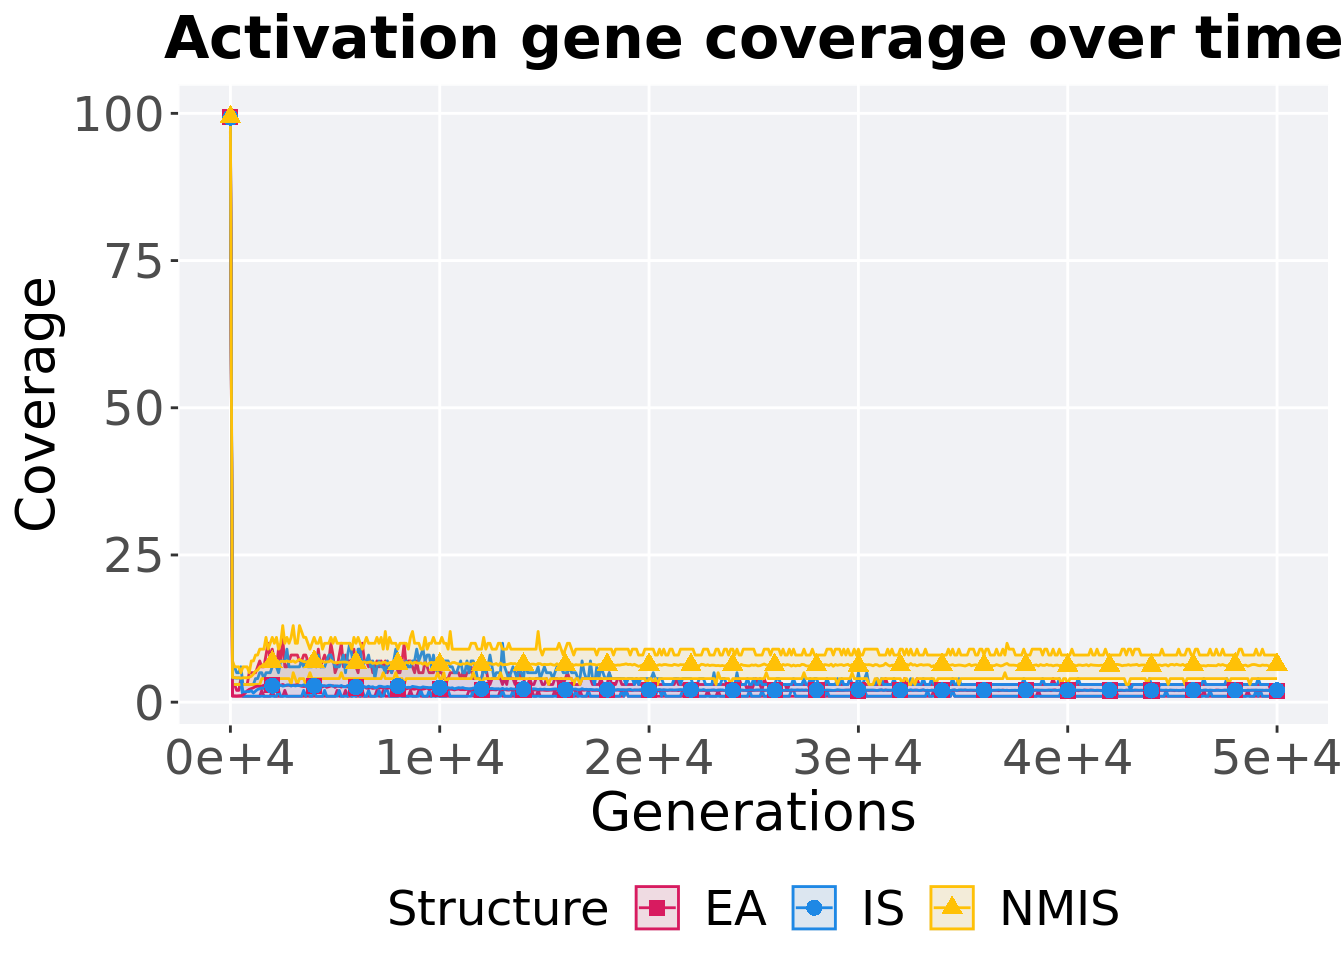
\includegraphics{demo_files/figure-latex/base-mpe-act-tru-ot-1.pdf}

\hypertarget{end-of-50000-generations-6}{%
\subsubsection{End of 50,000 generations}\label{end-of-50000-generations-6}}

Activation gene coverage in the population at the end of 50,000 generations.

\begin{Shaded}
\begin{Highlighting}[]
\CommentTok{### end of run}
\KeywordTok{filter}\NormalTok{(base_over_time, Diagnostic }\OperatorTok{==}\StringTok{ 'MULTIPATH_EXPLORATION'} \OperatorTok{&}\StringTok{ `}\DataTypeTok{Selection}\CharTok{\textbackslash{}n}\DataTypeTok{Scheme}\StringTok{`} \OperatorTok{==}\StringTok{ 'TRUNCATION'} \OperatorTok{&}\StringTok{ }\NormalTok{Generations }\OperatorTok{==}\StringTok{ }\DecValTok{50000}\NormalTok{) }\OperatorTok
\StringTok{  }\KeywordTok{ggplot}\NormalTok{(., }\KeywordTok{aes}\NormalTok{(}\DataTypeTok{x =}\NormalTok{ Structure, }\DataTypeTok{y =}\NormalTok{ pop_act_cov, }\DataTypeTok{color =}\NormalTok{ Structure, }\DataTypeTok{fill =}\NormalTok{ Structure, }\DataTypeTok{shape =}\NormalTok{ Structure)) }\OperatorTok{+}
\StringTok{  }\KeywordTok{geom_flat_violin}\NormalTok{(}\DataTypeTok{position =} \KeywordTok{position_nudge}\NormalTok{(}\DataTypeTok{x =} \FloatTok{.2}\NormalTok{, }\DataTypeTok{y =} \DecValTok{0}\NormalTok{), }\DataTypeTok{scale =} \StringTok{'width'}\NormalTok{, }\DataTypeTok{alpha =} \FloatTok{0.3}\NormalTok{) }\OperatorTok{+}
\StringTok{  }\KeywordTok{geom_point}\NormalTok{(}\DataTypeTok{position =} \KeywordTok{position_jitter}\NormalTok{(}\DataTypeTok{height =} \FloatTok{.05}\NormalTok{, }\DataTypeTok{width =} \FloatTok{.05}\NormalTok{), }\DataTypeTok{size =} \FloatTok{1.5}\NormalTok{, }\DataTypeTok{alpha =} \FloatTok{0.5}\NormalTok{) }\OperatorTok{+}
\StringTok{  }\KeywordTok{geom_boxplot}\NormalTok{(}\DataTypeTok{color =} \StringTok{'black'}\NormalTok{, }\DataTypeTok{width =} \FloatTok{.2}\NormalTok{, }\DataTypeTok{outlier.shape =} \OtherTok{NA}\NormalTok{, }\DataTypeTok{alpha =} \FloatTok{0.0}\NormalTok{) }\OperatorTok{+}
\StringTok{  }\KeywordTok{scale_shape_manual}\NormalTok{(}\DataTypeTok{values=}\NormalTok{SHAPE)}\OperatorTok{+}
\StringTok{  }\KeywordTok{scale_y_continuous}\NormalTok{(}
    \DataTypeTok{name=}\StringTok{"Coverage"}
\NormalTok{  ) }\OperatorTok{+}
\StringTok{  }\KeywordTok{scale_x_discrete}\NormalTok{(}
    \DataTypeTok{name=}\StringTok{"Structure"}
\NormalTok{  ) }\OperatorTok{+}
\StringTok{  }\KeywordTok{scale_colour_manual}\NormalTok{(}\DataTypeTok{values =}\NormalTok{ cb_palette) }\OperatorTok{+}
\StringTok{  }\KeywordTok{scale_fill_manual}\NormalTok{(}\DataTypeTok{values =}\NormalTok{ cb_palette) }\OperatorTok{+}
\StringTok{  }\KeywordTok{ggtitle}\NormalTok{(}\StringTok{'Final activation gene coverage'}\NormalTok{)}\OperatorTok{+}
\StringTok{  }\NormalTok{p_theme }\OperatorTok{+}\StringTok{ }\KeywordTok{coord_flip}\NormalTok{()}
\end{Highlighting}
\end{Shaded}

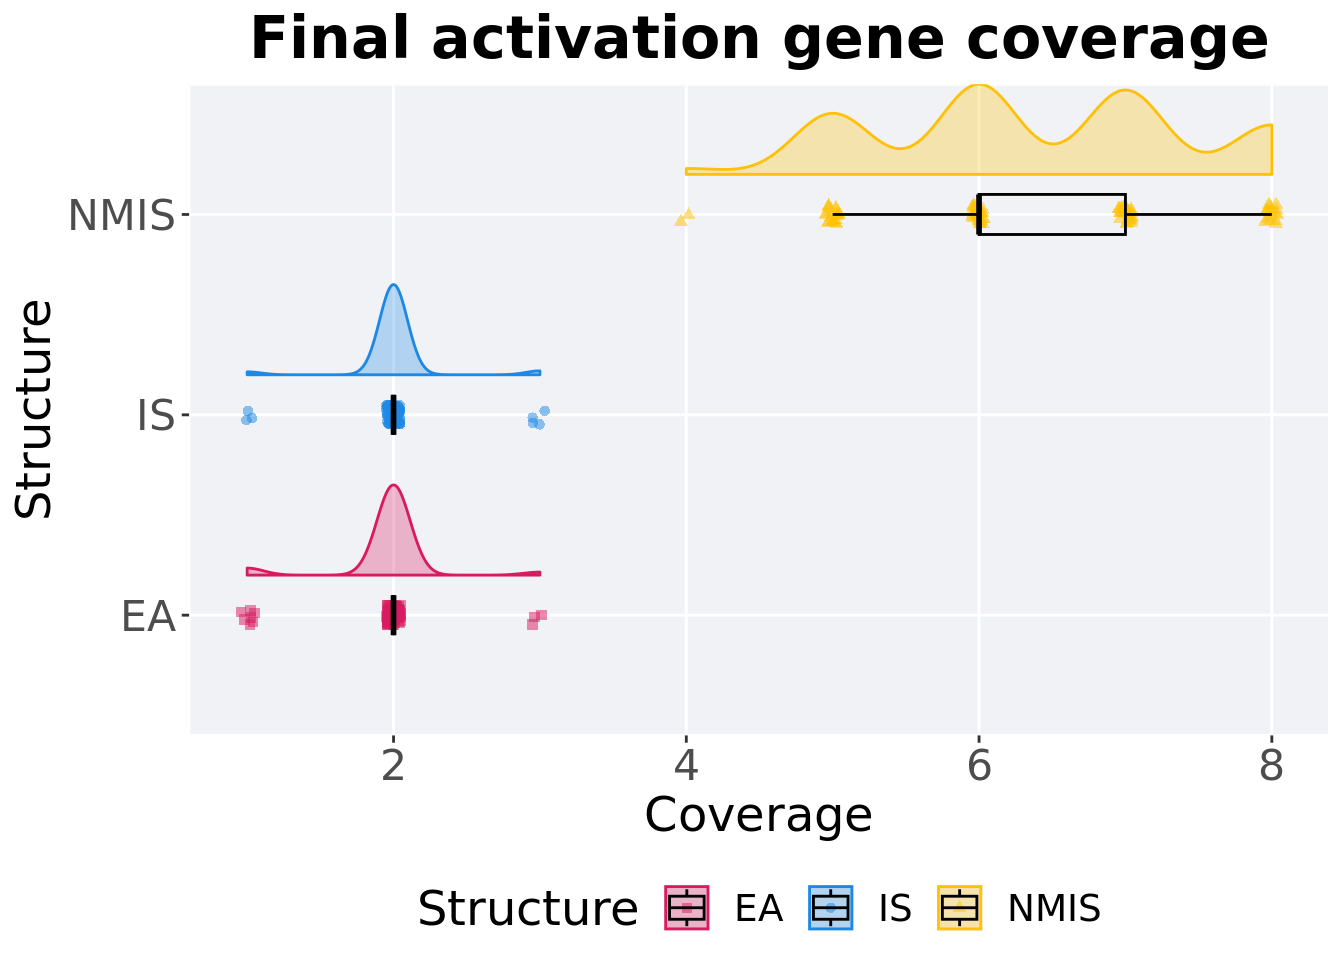
\includegraphics{demo_files/figure-latex/base-mpe-act-tru-end-1.pdf}

\hypertarget{stats-20}{%
\paragraph{Stats}\label{stats-20}}

Summary statistics for activation gene coverage.

\begin{Shaded}
\begin{Highlighting}[]
\NormalTok{coverage =}\StringTok{ }\KeywordTok{filter}\NormalTok{(base_over_time, Diagnostic }\OperatorTok{==}\StringTok{ 'MULTIPATH_EXPLORATION'} \OperatorTok{&}\StringTok{ `}\DataTypeTok{Selection}\CharTok{\textbackslash{}n}\DataTypeTok{Scheme}\StringTok{`} \OperatorTok{==}\StringTok{ 'TRUNCATION'} \OperatorTok{&}\StringTok{ }\NormalTok{Generations }\OperatorTok{==}\StringTok{ }\DecValTok{50000}\NormalTok{)}
\NormalTok{coverage }\OperatorTok
\StringTok{  }\KeywordTok{group_by}\NormalTok{(Structure) }\OperatorTok
\StringTok{  }\NormalTok{dplyr}\OperatorTok{::}\KeywordTok{summarise}\NormalTok{(}
    \DataTypeTok{count =} \KeywordTok{n}\NormalTok{(),}
    \DataTypeTok{na_cnt =} \KeywordTok{sum}\NormalTok{(}\KeywordTok{is.na}\NormalTok{(pop_act_cov)),}
    \DataTypeTok{min =} \KeywordTok{min}\NormalTok{(pop_act_cov, }\DataTypeTok{na.rm =} \OtherTok{TRUE}\NormalTok{),}
    \DataTypeTok{median =} \KeywordTok{median}\NormalTok{(pop_act_cov, }\DataTypeTok{na.rm =} \OtherTok{TRUE}\NormalTok{),}
    \DataTypeTok{mean =} \KeywordTok{mean}\NormalTok{(pop_act_cov, }\DataTypeTok{na.rm =} \OtherTok{TRUE}\NormalTok{),}
    \DataTypeTok{max =} \KeywordTok{max}\NormalTok{(pop_act_cov, }\DataTypeTok{na.rm =} \OtherTok{TRUE}\NormalTok{),}
    \DataTypeTok{IQR =} \KeywordTok{IQR}\NormalTok{(pop_act_cov, }\DataTypeTok{na.rm =} \OtherTok{TRUE}\NormalTok{)}
\NormalTok{  )}
\end{Highlighting}
\end{Shaded}

\begin{verbatim}
## # A tibble: 3 x 8
##   Structure count na_cnt   min median  mean   max   IQR
##   <fct>     <int>  <int> <int>  <dbl> <dbl> <int> <dbl>
## 1 EA          100      0     1      2  1.96     3     0
## 2 IS          100      0     1      2  2.01     3     0
## 3 NMIS        100      0     4      6  6.38     8     1
\end{verbatim}

Kruskal--Wallis test provides evidence of difference among activation gene coverage.

\begin{Shaded}
\begin{Highlighting}[]
\KeywordTok{kruskal.test}\NormalTok{(pop_act_cov }\OperatorTok{~}\StringTok{ }\NormalTok{Structure, }\DataTypeTok{data =}\NormalTok{ coverage)}
\end{Highlighting}
\end{Shaded}

\begin{verbatim}
## 
##  Kruskal-Wallis rank sum test
## 
## data:  pop_act_cov by Structure
## Kruskal-Wallis chi-squared = 258.93, df = 2, p-value < 2.2e-16
\end{verbatim}

Results for post-hoc Wilcoxon rank-sum test with a Bonferroni correction on activation gene coverage.

\begin{Shaded}
\begin{Highlighting}[]
\KeywordTok{pairwise.wilcox.test}\NormalTok{(}\DataTypeTok{x =}\NormalTok{ coverage}\OperatorTok{$}\NormalTok{pop_act_cov, }\DataTypeTok{g =}\NormalTok{ coverage}\OperatorTok{$}\NormalTok{Structure, }\DataTypeTok{p.adjust.method =} \StringTok{"bonferroni"}\NormalTok{,}
                     \DataTypeTok{paired =} \OtherTok{FALSE}\NormalTok{, }\DataTypeTok{conf.int =} \OtherTok{FALSE}\NormalTok{, }\DataTypeTok{alternative =} \StringTok{'g'}\NormalTok{)}
\end{Highlighting}
\end{Shaded}

\begin{verbatim}
## 
##  Pairwise comparisons using Wilcoxon rank sum test with continuity correction 
## 
## data:  coverage$pop_act_cov and coverage$Structure 
## 
##      EA     IS    
## IS   0.34   -     
## NMIS <2e-16 <2e-16
## 
## P value adjustment method: bonferroni
\end{verbatim}

\hypertarget{tournament-selection-3}{%
\section{Tournament selection}\label{tournament-selection-3}}

Here we analyze how the different population structures affect tournament selection (size 8) on the contradictory objectives diagnostic.

\hypertarget{performance-1}{%
\subsection{Performance}\label{performance-1}}

\hypertarget{performance-over-time-7}{%
\subsubsection{Performance over time}\label{performance-over-time-7}}

\begin{Shaded}
\begin{Highlighting}[]
\NormalTok{lines =}\StringTok{ }\KeywordTok{filter}\NormalTok{(base_over_time, Diagnostic }\OperatorTok{==}\StringTok{ 'MULTIPATH_EXPLORATION'} \OperatorTok{&}\StringTok{ `}\DataTypeTok{Selection}\CharTok{\textbackslash{}n}\DataTypeTok{Scheme}\StringTok{`} \OperatorTok{==}\StringTok{ 'TOURNAMENT'}\NormalTok{) }\OperatorTok
\StringTok{  }\KeywordTok{group_by}\NormalTok{(Structure, Generations) }\OperatorTok
\StringTok{  }\NormalTok{dplyr}\OperatorTok{::}\KeywordTok{summarise}\NormalTok{(}
    \DataTypeTok{min =} \KeywordTok{min}\NormalTok{(pop_fit_max) }\OperatorTok{/}\StringTok{ }\NormalTok{DIMENSIONALITY,}
    \DataTypeTok{mean =} \KeywordTok{mean}\NormalTok{(pop_fit_max) }\OperatorTok{/}\StringTok{ }\NormalTok{DIMENSIONALITY,}
    \DataTypeTok{max =} \KeywordTok{max}\NormalTok{(pop_fit_max) }\OperatorTok{/}\StringTok{ }\NormalTok{DIMENSIONALITY}
\NormalTok{  )}
\KeywordTok{ggplot}\NormalTok{(lines, }\KeywordTok{aes}\NormalTok{(}\DataTypeTok{x=}\NormalTok{Generations, }\DataTypeTok{y=}\NormalTok{mean, }\DataTypeTok{group =}\NormalTok{ Structure, }\DataTypeTok{fill =}\NormalTok{ Structure, }\DataTypeTok{color =}\NormalTok{ Structure, }\DataTypeTok{shape =}\NormalTok{ Structure)) }\OperatorTok{+}
\StringTok{  }\KeywordTok{geom_ribbon}\NormalTok{(}\KeywordTok{aes}\NormalTok{(}\DataTypeTok{ymin =}\NormalTok{ min, }\DataTypeTok{ymax =}\NormalTok{ max), }\DataTypeTok{alpha =} \FloatTok{0.1}\NormalTok{) }\OperatorTok{+}
\StringTok{  }\KeywordTok{geom_line}\NormalTok{(}\DataTypeTok{size =} \FloatTok{0.5}\NormalTok{) }\OperatorTok{+}
\StringTok{  }\KeywordTok{geom_point}\NormalTok{(}\DataTypeTok{data =} \KeywordTok{filter}\NormalTok{(lines, Generations }\OperatorTok\StringTok{ }\DecValTok{2000} \OperatorTok{==}\StringTok{ }\DecValTok{0}\NormalTok{), }\DataTypeTok{size =} \FloatTok{2.5}\NormalTok{, }\DataTypeTok{stroke =} \FloatTok{2.0}\NormalTok{, }\DataTypeTok{alpha =} \FloatTok{1.0}\NormalTok{) }\OperatorTok{+}
\StringTok{  }\KeywordTok{scale_y_continuous}\NormalTok{(}
    \DataTypeTok{name=}\StringTok{"Average trait score"}
\NormalTok{  ) }\OperatorTok{+}
\StringTok{  }\KeywordTok{scale_x_continuous}\NormalTok{(}
    \DataTypeTok{name=}\StringTok{"Generations"}\NormalTok{,}
    \DataTypeTok{limits=}\KeywordTok{c}\NormalTok{(}\DecValTok{0}\NormalTok{, }\DecValTok{50000}\NormalTok{),}
    \DataTypeTok{breaks=}\KeywordTok{c}\NormalTok{(}\DecValTok{0}\NormalTok{, }\DecValTok{10000}\NormalTok{, }\DecValTok{20000}\NormalTok{, }\DecValTok{30000}\NormalTok{, }\DecValTok{40000}\NormalTok{, }\DecValTok{50000}\NormalTok{),}
    \DataTypeTok{labels=}\KeywordTok{c}\NormalTok{(}\StringTok{"0e+4"}\NormalTok{, }\StringTok{"1e+4"}\NormalTok{, }\StringTok{"2e+4"}\NormalTok{, }\StringTok{"3e+4"}\NormalTok{, }\StringTok{"4e+4"}\NormalTok{, }\StringTok{"5e+4"}\NormalTok{)}

\NormalTok{  ) }\OperatorTok{+}
\StringTok{  }\KeywordTok{scale_shape_manual}\NormalTok{(}\DataTypeTok{values=}\NormalTok{SHAPE)}\OperatorTok{+}
\StringTok{  }\KeywordTok{scale_colour_manual}\NormalTok{(}\DataTypeTok{values =}\NormalTok{ cb_palette) }\OperatorTok{+}
\StringTok{  }\KeywordTok{scale_fill_manual}\NormalTok{(}\DataTypeTok{values =}\NormalTok{ cb_palette) }\OperatorTok{+}
\StringTok{  }\KeywordTok{ggtitle}\NormalTok{(}\StringTok{"Performance over time"}\NormalTok{) }\OperatorTok{+}
\StringTok{  }\NormalTok{p_theme}
\end{Highlighting}
\end{Shaded}

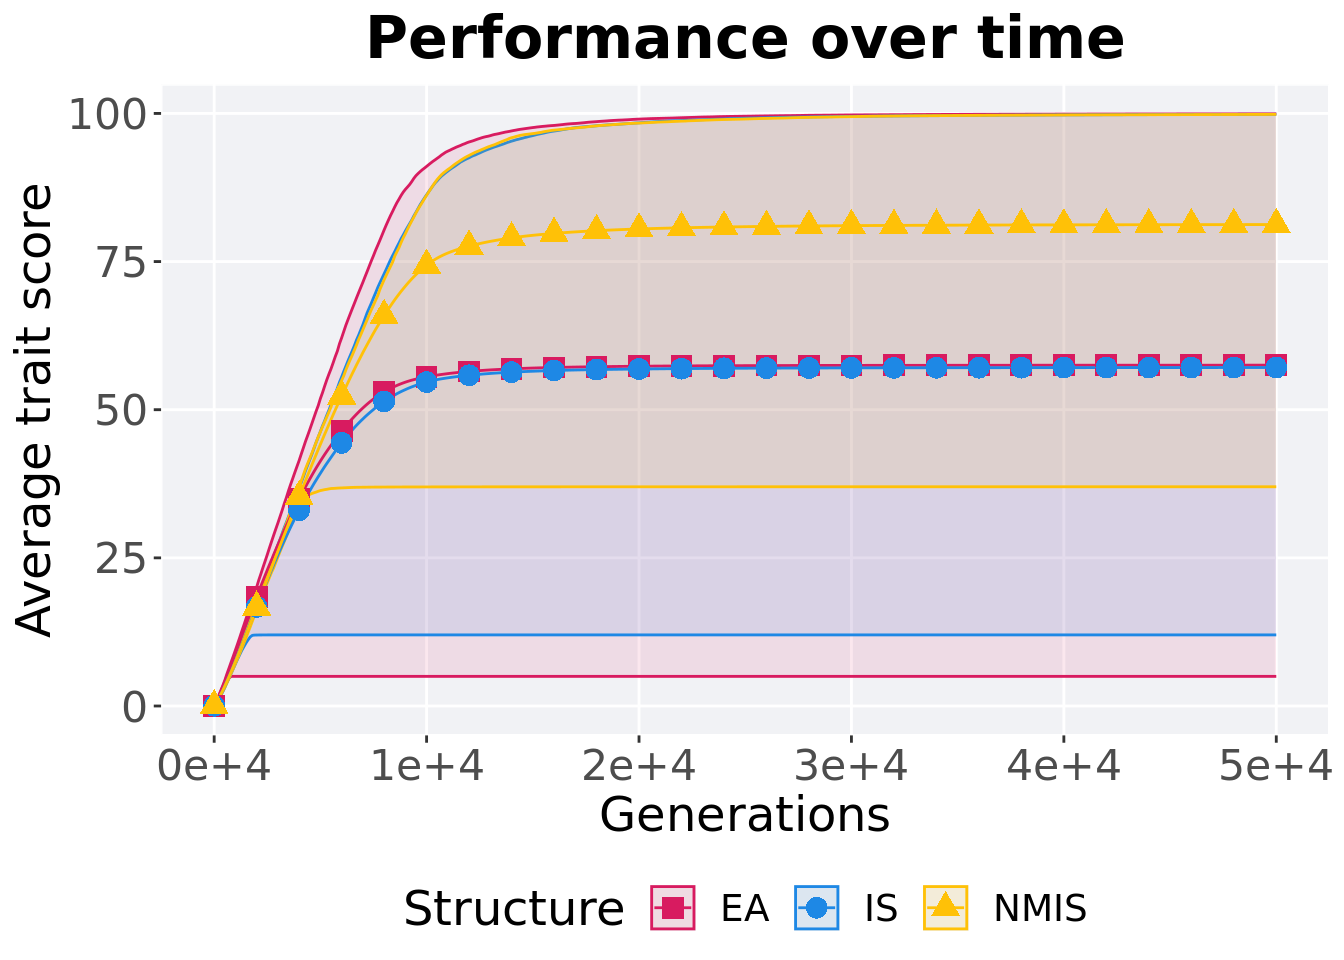
\includegraphics{demo_files/figure-latex/base-tor-mpe-perf-1.pdf}

\hypertarget{best-performance-2}{%
\subsubsection{Best performance}\label{best-performance-2}}

First generation a satisfactory solution is found throughout the 50,000 generations.

\begin{Shaded}
\begin{Highlighting}[]
\KeywordTok{filter}\NormalTok{(base_best, Diagnostic }\OperatorTok{==}\StringTok{ 'MULTIPATH_EXPLORATION'} \OperatorTok{&}\StringTok{ `}\DataTypeTok{Selection}\CharTok{\textbackslash{}n}\DataTypeTok{Scheme}\StringTok{`} \OperatorTok{==}\StringTok{ 'TOURNAMENT'} \OperatorTok{&}\StringTok{ }\NormalTok{VAR }\OperatorTok{==}\StringTok{ 'pop_fit_max'}\NormalTok{) }\OperatorTok
\StringTok{  }\KeywordTok{ggplot}\NormalTok{(., }\KeywordTok{aes}\NormalTok{(}\DataTypeTok{x =}\NormalTok{ Structure, }\DataTypeTok{y =}\NormalTok{ VAL }\OperatorTok{/}\StringTok{ }\NormalTok{DIMENSIONALITY, }\DataTypeTok{color =}\NormalTok{ Structure, }\DataTypeTok{fill =}\NormalTok{ Structure, }\DataTypeTok{shape =}\NormalTok{ Structure)) }\OperatorTok{+}
\StringTok{  }\KeywordTok{geom_flat_violin}\NormalTok{(}\DataTypeTok{position =} \KeywordTok{position_nudge}\NormalTok{(}\DataTypeTok{x =} \FloatTok{.2}\NormalTok{, }\DataTypeTok{y =} \DecValTok{0}\NormalTok{), }\DataTypeTok{scale =} \StringTok{'width'}\NormalTok{, }\DataTypeTok{alpha =} \FloatTok{0.2}\NormalTok{) }\OperatorTok{+}
\StringTok{  }\KeywordTok{geom_point}\NormalTok{(}\DataTypeTok{position =} \KeywordTok{position_jitter}\NormalTok{(}\DataTypeTok{width =} \FloatTok{.1}\NormalTok{), }\DataTypeTok{size =} \FloatTok{1.5}\NormalTok{, }\DataTypeTok{alpha =} \FloatTok{1.0}\NormalTok{) }\OperatorTok{+}
\StringTok{  }\KeywordTok{geom_boxplot}\NormalTok{(}\DataTypeTok{color =} \StringTok{'black'}\NormalTok{, }\DataTypeTok{width =} \FloatTok{.2}\NormalTok{, }\DataTypeTok{outlier.shape =} \OtherTok{NA}\NormalTok{, }\DataTypeTok{alpha =} \FloatTok{0.0}\NormalTok{) }\OperatorTok{+}
\StringTok{  }\KeywordTok{scale_y_continuous}\NormalTok{(}
    \DataTypeTok{name=}\StringTok{"Average trait score"}
\NormalTok{  ) }\OperatorTok{+}
\StringTok{  }\KeywordTok{scale_x_discrete}\NormalTok{(}
    \DataTypeTok{name=}\StringTok{"Structure"}
\NormalTok{  )}\OperatorTok{+}
\StringTok{  }\KeywordTok{scale_shape_manual}\NormalTok{(}\DataTypeTok{values=}\NormalTok{SHAPE)}\OperatorTok{+}
\StringTok{  }\KeywordTok{scale_colour_manual}\NormalTok{(}\DataTypeTok{values =}\NormalTok{ cb_palette, ) }\OperatorTok{+}
\StringTok{  }\KeywordTok{scale_fill_manual}\NormalTok{(}\DataTypeTok{values =}\NormalTok{ cb_palette) }\OperatorTok{+}
\StringTok{  }\KeywordTok{ggtitle}\NormalTok{(}\StringTok{'Best performance'}\NormalTok{)}\OperatorTok{+}
\StringTok{  }\NormalTok{p_theme }\OperatorTok{+}\StringTok{ }\KeywordTok{coord_flip}\NormalTok{()}
\end{Highlighting}
\end{Shaded}

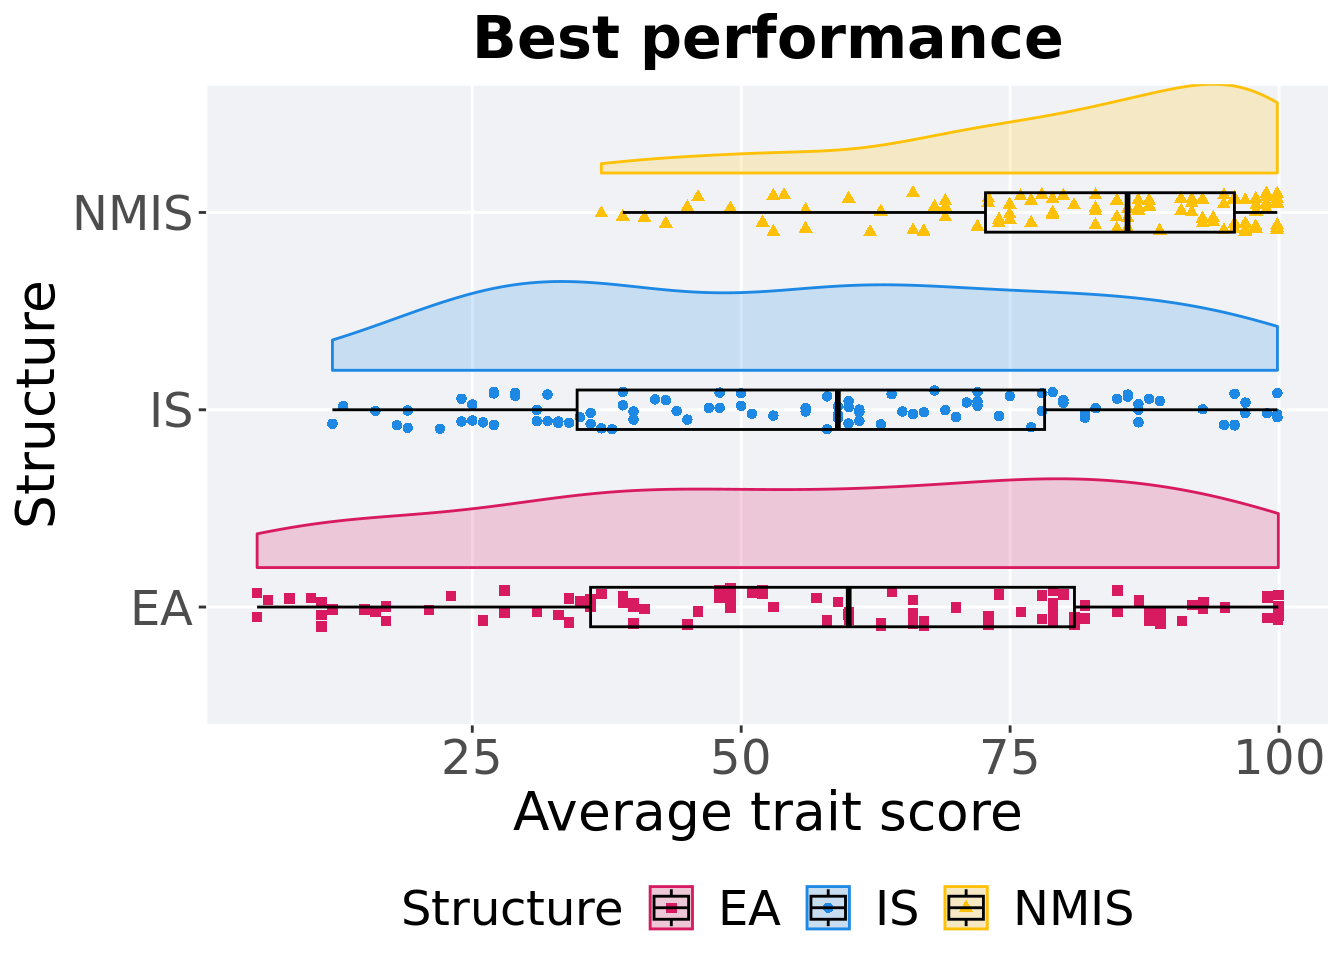
\includegraphics{demo_files/figure-latex/base-tor-mpe-per-bst-1.pdf}

\hypertarget{stats-21}{%
\paragraph{Stats}\label{stats-21}}

Summary statistics for the first generation a satisfactory solution is found.

\begin{Shaded}
\begin{Highlighting}[]
\NormalTok{performance =}\StringTok{ }\KeywordTok{filter}\NormalTok{(base_best, Diagnostic }\OperatorTok{==}\StringTok{ 'MULTIPATH_EXPLORATION'} \OperatorTok{&}\StringTok{ `}\DataTypeTok{Selection}\CharTok{\textbackslash{}n}\DataTypeTok{Scheme}\StringTok{`} \OperatorTok{==}\StringTok{ 'TOURNAMENT'} \OperatorTok{&}\StringTok{ }\NormalTok{VAR }\OperatorTok{==}\StringTok{ 'pop_fit_max'}\NormalTok{)}
\NormalTok{performance }\OperatorTok
\StringTok{  }\KeywordTok{group_by}\NormalTok{(Structure) }\OperatorTok
\StringTok{  }\NormalTok{dplyr}\OperatorTok{::}\KeywordTok{summarise}\NormalTok{(}
    \DataTypeTok{count =} \KeywordTok{n}\NormalTok{(),}
    \DataTypeTok{na_cnt =} \KeywordTok{sum}\NormalTok{(}\KeywordTok{is.na}\NormalTok{(VAL)),}
    \DataTypeTok{min =} \KeywordTok{min}\NormalTok{(VAL, }\DataTypeTok{na.rm =} \OtherTok{TRUE}\NormalTok{) }\OperatorTok{/}\StringTok{ }\NormalTok{DIMENSIONALITY,}
    \DataTypeTok{median =} \KeywordTok{median}\NormalTok{(VAL, }\DataTypeTok{na.rm =} \OtherTok{TRUE}\NormalTok{) }\OperatorTok{/}\StringTok{ }\NormalTok{DIMENSIONALITY,}
    \DataTypeTok{mean =} \KeywordTok{mean}\NormalTok{(VAL, }\DataTypeTok{na.rm =} \OtherTok{TRUE}\NormalTok{) }\OperatorTok{/}\StringTok{ }\NormalTok{DIMENSIONALITY,}
    \DataTypeTok{max =} \KeywordTok{max}\NormalTok{(VAL, }\DataTypeTok{na.rm =} \OtherTok{TRUE}\NormalTok{) }\OperatorTok{/}\StringTok{ }\NormalTok{DIMENSIONALITY,}
    \DataTypeTok{IQR =} \KeywordTok{IQR}\NormalTok{(VAL, }\DataTypeTok{na.rm =} \OtherTok{TRUE}\NormalTok{) }\OperatorTok{/}\StringTok{ }\NormalTok{DIMENSIONALITY}
\NormalTok{  )}
\end{Highlighting}
\end{Shaded}

\begin{verbatim}
## # A tibble: 3 x 8
##   Structure count na_cnt   min median  mean   max   IQR
##   <fct>     <int>  <int> <dbl>  <dbl> <dbl> <dbl> <dbl>
## 1 EA          100      0   5     60.0  57.5  99.9  45.0
## 2 IS          100      0  12     59.0  57.1  99.9  43.5
## 3 NMIS        100      0  37.0   85.9  81.2  99.8  23.1
\end{verbatim}

Kruskal--Wallis test provides evidence of difference among selection schemes.

\begin{Shaded}
\begin{Highlighting}[]
\KeywordTok{kruskal.test}\NormalTok{(VAL }\OperatorTok{~}\StringTok{ }\NormalTok{Structure, }\DataTypeTok{data =}\NormalTok{ performance)}
\end{Highlighting}
\end{Shaded}

\begin{verbatim}
## 
##  Kruskal-Wallis rank sum test
## 
## data:  VAL by Structure
## Kruskal-Wallis chi-squared = 52.543, df = 2, p-value = 3.895e-12
\end{verbatim}

Results for post-hoc Wilcoxon rank-sum test with a Bonferroni correction.

\begin{Shaded}
\begin{Highlighting}[]
\KeywordTok{pairwise.wilcox.test}\NormalTok{(}\DataTypeTok{x =}\NormalTok{ performance}\OperatorTok{$}\NormalTok{VAL, }\DataTypeTok{g =}\NormalTok{ performance}\OperatorTok{$}\NormalTok{Structure, }\DataTypeTok{p.adjust.method =} \StringTok{"bonferroni"}\NormalTok{,}
                     \DataTypeTok{paired =} \OtherTok{FALSE}\NormalTok{, }\DataTypeTok{conf.int =} \OtherTok{FALSE}\NormalTok{, }\DataTypeTok{alternative =} \StringTok{'g'}\NormalTok{)}
\end{Highlighting}
\end{Shaded}

\begin{verbatim}
## 
##  Pairwise comparisons using Wilcoxon rank sum test with continuity correction 
## 
## data:  performance$VAL and performance$Structure 
## 
##      EA      IS     
## IS   1       -      
## NMIS 5.9e-09 5.3e-11
## 
## P value adjustment method: bonferroni
\end{verbatim}

\hypertarget{final-performance-2}{%
\subsubsection{Final performance}\label{final-performance-2}}

First generation a satisfactory solution is found throughout the 50,000 generations.

\begin{Shaded}
\begin{Highlighting}[]
\KeywordTok{filter}\NormalTok{(base_over_time, Diagnostic }\OperatorTok{==}\StringTok{ 'MULTIPATH_EXPLORATION'} \OperatorTok{&}\StringTok{ `}\DataTypeTok{Selection}\CharTok{\textbackslash{}n}\DataTypeTok{Scheme}\StringTok{`} \OperatorTok{==}\StringTok{ 'TOURNAMENT'} \OperatorTok{&}\StringTok{ }\NormalTok{Generations }\OperatorTok{==}\StringTok{ }\DecValTok{50000}\NormalTok{) }\OperatorTok
\StringTok{  }\KeywordTok{ggplot}\NormalTok{(., }\KeywordTok{aes}\NormalTok{(}\DataTypeTok{x =}\NormalTok{ Structure, }\DataTypeTok{y =}\NormalTok{ pop_fit_max }\OperatorTok{/}\StringTok{ }\NormalTok{DIMENSIONALITY, }\DataTypeTok{color =}\NormalTok{ Structure, }\DataTypeTok{fill =}\NormalTok{ Structure, }\DataTypeTok{shape =}\NormalTok{ Structure)) }\OperatorTok{+}
\StringTok{  }\KeywordTok{geom_flat_violin}\NormalTok{(}\DataTypeTok{position =} \KeywordTok{position_nudge}\NormalTok{(}\DataTypeTok{x =} \FloatTok{.2}\NormalTok{, }\DataTypeTok{y =} \DecValTok{0}\NormalTok{), }\DataTypeTok{scale =} \StringTok{'width'}\NormalTok{, }\DataTypeTok{alpha =} \FloatTok{0.2}\NormalTok{) }\OperatorTok{+}
\StringTok{  }\KeywordTok{geom_point}\NormalTok{(}\DataTypeTok{position =} \KeywordTok{position_jitter}\NormalTok{(}\DataTypeTok{width =} \FloatTok{.1}\NormalTok{), }\DataTypeTok{size =} \FloatTok{1.5}\NormalTok{, }\DataTypeTok{alpha =} \FloatTok{1.0}\NormalTok{) }\OperatorTok{+}
\StringTok{  }\KeywordTok{geom_boxplot}\NormalTok{(}\DataTypeTok{color =} \StringTok{'black'}\NormalTok{, }\DataTypeTok{width =} \FloatTok{.2}\NormalTok{, }\DataTypeTok{outlier.shape =} \OtherTok{NA}\NormalTok{, }\DataTypeTok{alpha =} \FloatTok{0.0}\NormalTok{) }\OperatorTok{+}
\StringTok{  }\KeywordTok{scale_y_continuous}\NormalTok{(}
    \DataTypeTok{name=}\StringTok{"Average trait score"}
\NormalTok{  ) }\OperatorTok{+}
\StringTok{  }\KeywordTok{scale_x_discrete}\NormalTok{(}
    \DataTypeTok{name=}\StringTok{"Structure"}
\NormalTok{  )}\OperatorTok{+}
\StringTok{  }\KeywordTok{scale_shape_manual}\NormalTok{(}\DataTypeTok{values=}\NormalTok{SHAPE)}\OperatorTok{+}
\StringTok{  }\KeywordTok{scale_colour_manual}\NormalTok{(}\DataTypeTok{values =}\NormalTok{ cb_palette, ) }\OperatorTok{+}
\StringTok{  }\KeywordTok{scale_fill_manual}\NormalTok{(}\DataTypeTok{values =}\NormalTok{ cb_palette) }\OperatorTok{+}
\StringTok{  }\KeywordTok{ggtitle}\NormalTok{(}\StringTok{'Final performance'}\NormalTok{)}\OperatorTok{+}
\StringTok{  }\NormalTok{p_theme }\OperatorTok{+}\StringTok{ }\KeywordTok{coord_flip}\NormalTok{()}
\end{Highlighting}
\end{Shaded}

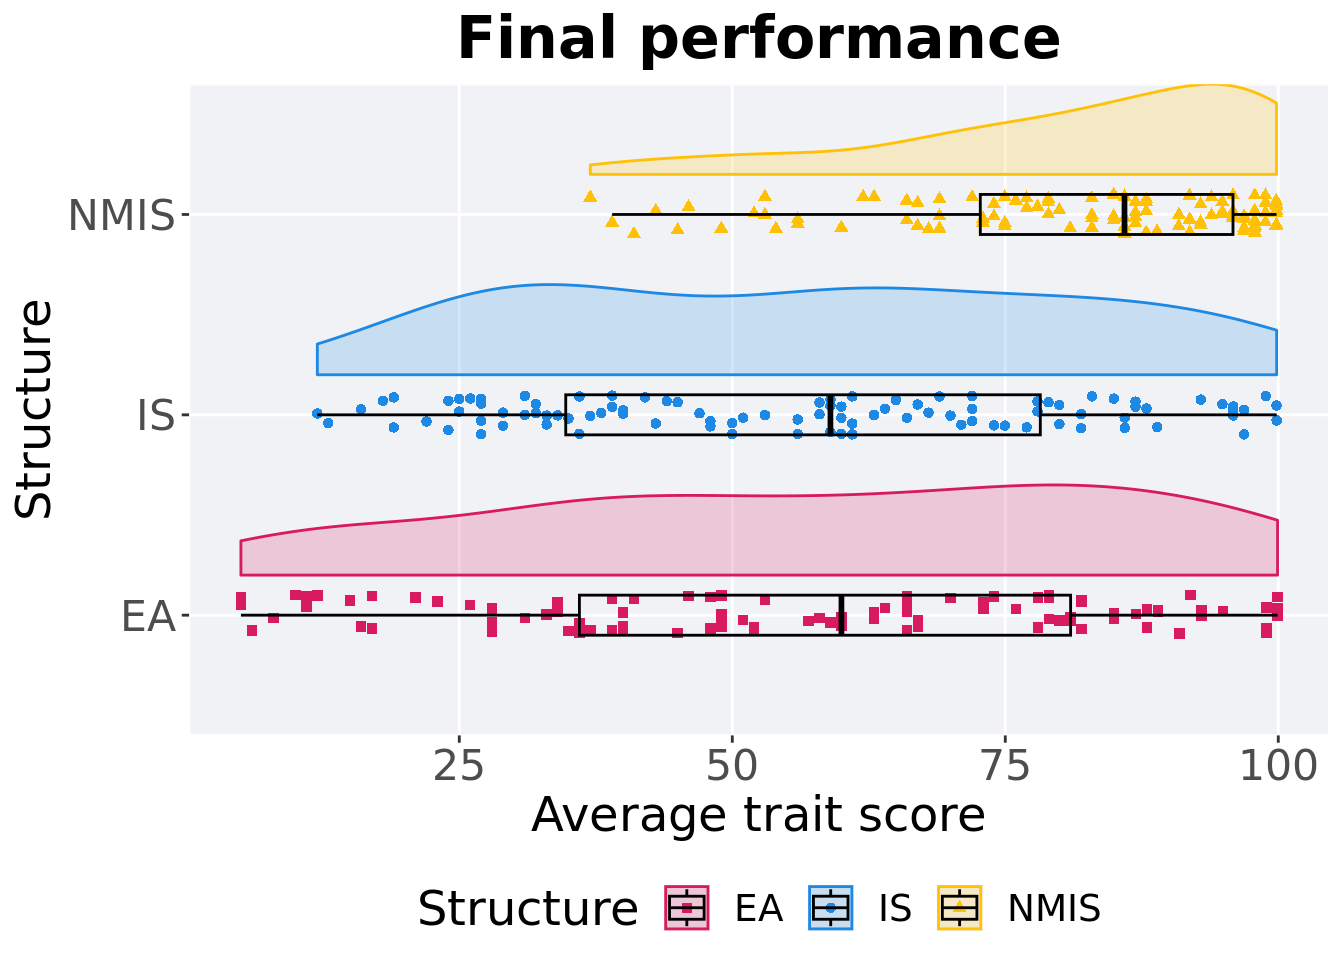
\includegraphics{demo_files/figure-latex/base-tor-mpe-per-end-1.pdf}

\hypertarget{stats-22}{%
\paragraph{Stats}\label{stats-22}}

Summary statistics for the first generation a satisfactory solution is found.

\begin{Shaded}
\begin{Highlighting}[]
\NormalTok{performance =}\StringTok{ }\KeywordTok{filter}\NormalTok{(base_over_time, Diagnostic }\OperatorTok{==}\StringTok{ 'MULTIPATH_EXPLORATION'} \OperatorTok{&}\StringTok{ `}\DataTypeTok{Selection}\CharTok{\textbackslash{}n}\DataTypeTok{Scheme}\StringTok{`} \OperatorTok{==}\StringTok{ 'TOURNAMENT'} \OperatorTok{&}\StringTok{ }\NormalTok{Generations }\OperatorTok{==}\StringTok{ }\DecValTok{50000}\NormalTok{)}
\NormalTok{performance }\OperatorTok
\StringTok{  }\KeywordTok{group_by}\NormalTok{(Structure) }\OperatorTok
\StringTok{  }\NormalTok{dplyr}\OperatorTok{::}\KeywordTok{summarise}\NormalTok{(}
    \DataTypeTok{count =} \KeywordTok{n}\NormalTok{(),}
    \DataTypeTok{na_cnt =} \KeywordTok{sum}\NormalTok{(}\KeywordTok{is.na}\NormalTok{(pop_fit_max)),}
    \DataTypeTok{min =} \KeywordTok{min}\NormalTok{(pop_fit_max }\OperatorTok{/}\StringTok{ }\NormalTok{DIMENSIONALITY, }\DataTypeTok{na.rm =} \OtherTok{TRUE}\NormalTok{),}
    \DataTypeTok{median =} \KeywordTok{median}\NormalTok{(pop_fit_max }\OperatorTok{/}\StringTok{ }\NormalTok{DIMENSIONALITY, }\DataTypeTok{na.rm =} \OtherTok{TRUE}\NormalTok{),}
    \DataTypeTok{mean =} \KeywordTok{mean}\NormalTok{(pop_fit_max }\OperatorTok{/}\StringTok{ }\NormalTok{DIMENSIONALITY, }\DataTypeTok{na.rm =} \OtherTok{TRUE}\NormalTok{),}
    \DataTypeTok{max =} \KeywordTok{max}\NormalTok{(pop_fit_max }\OperatorTok{/}\StringTok{ }\NormalTok{DIMENSIONALITY, }\DataTypeTok{na.rm =} \OtherTok{TRUE}\NormalTok{),}
    \DataTypeTok{IQR =} \KeywordTok{IQR}\NormalTok{(pop_fit_max }\OperatorTok{/}\StringTok{ }\NormalTok{DIMENSIONALITY, }\DataTypeTok{na.rm =} \OtherTok{TRUE}\NormalTok{)}
\NormalTok{  )}
\end{Highlighting}
\end{Shaded}

\begin{verbatim}
## # A tibble: 3 x 8
##   Structure count na_cnt   min median  mean   max   IQR
##   <fct>     <int>  <int> <dbl>  <dbl> <dbl> <dbl> <dbl>
## 1 EA          100      0   5     60.0  57.5  99.9  45.0
## 2 IS          100      0  12     59.0  57.1  99.9  43.5
## 3 NMIS        100      0  37.0   85.9  81.2  99.8  23.1
\end{verbatim}

Kruskal--Wallis test provides evidence of difference among selection schemes.

\begin{Shaded}
\begin{Highlighting}[]
\KeywordTok{kruskal.test}\NormalTok{(pop_fit_max }\OperatorTok{~}\StringTok{ }\NormalTok{Structure, }\DataTypeTok{data =}\NormalTok{ performance)}
\end{Highlighting}
\end{Shaded}

\begin{verbatim}
## 
##  Kruskal-Wallis rank sum test
## 
## data:  pop_fit_max by Structure
## Kruskal-Wallis chi-squared = 52.543, df = 2, p-value = 3.895e-12
\end{verbatim}

Results for post-hoc Wilcoxon rank-sum test with a Bonferroni correction.

\begin{Shaded}
\begin{Highlighting}[]
\KeywordTok{pairwise.wilcox.test}\NormalTok{(}\DataTypeTok{x =}\NormalTok{ performance}\OperatorTok{$}\NormalTok{pop_fit_max, }\DataTypeTok{g =}\NormalTok{ performance}\OperatorTok{$}\NormalTok{Structure, }\DataTypeTok{p.adjust.method =} \StringTok{"bonferroni"}\NormalTok{,}
                     \DataTypeTok{paired =} \OtherTok{FALSE}\NormalTok{, }\DataTypeTok{conf.int =} \OtherTok{FALSE}\NormalTok{, }\DataTypeTok{alternative =} \StringTok{'g'}\NormalTok{)}
\end{Highlighting}
\end{Shaded}

\begin{verbatim}
## 
##  Pairwise comparisons using Wilcoxon rank sum test with continuity correction 
## 
## data:  performance$pop_fit_max and performance$Structure 
## 
##      EA      IS     
## IS   1       -      
## NMIS 5.9e-09 5.3e-11
## 
## P value adjustment method: bonferroni
\end{verbatim}

\hypertarget{generation-satisfactory-solution-found-7}{%
\subsection{Generation satisfactory solution found}\label{generation-satisfactory-solution-found-7}}

First generation a satisfactory solution is found throughout the 50,000 generations.

\begin{Shaded}
\begin{Highlighting}[]
\KeywordTok{filter}\NormalTok{(base_ssf, Diagnostic }\OperatorTok{==}\StringTok{ 'MULTIPATH_EXPLORATION'} \OperatorTok{&}\StringTok{ `}\DataTypeTok{Selection}\CharTok{\textbackslash{}n}\DataTypeTok{Scheme}\StringTok{`} \OperatorTok{==}\StringTok{ 'TOURNAMENT'}\OperatorTok{&}\StringTok{ }\NormalTok{Generations }\OperatorTok{<=}\StringTok{ }\NormalTok{GENERATIONS) }\OperatorTok
\StringTok{  }\KeywordTok{ggplot}\NormalTok{(., }\KeywordTok{aes}\NormalTok{(}\DataTypeTok{x =}\NormalTok{ Structure, }\DataTypeTok{y =}\NormalTok{ Generations, }\DataTypeTok{color =}\NormalTok{ Structure, }\DataTypeTok{fill =}\NormalTok{ Structure, }\DataTypeTok{shape =}\NormalTok{ Structure)) }\OperatorTok{+}
\StringTok{    }\KeywordTok{geom_flat_violin}\NormalTok{(}\DataTypeTok{position =} \KeywordTok{position_nudge}\NormalTok{(}\DataTypeTok{x =} \FloatTok{.2}\NormalTok{, }\DataTypeTok{y =} \DecValTok{0}\NormalTok{), }\DataTypeTok{scale =} \StringTok{'width'}\NormalTok{, }\DataTypeTok{alpha =} \FloatTok{0.2}\NormalTok{) }\OperatorTok{+}
\StringTok{  }\KeywordTok{geom_point}\NormalTok{(}\DataTypeTok{position =} \KeywordTok{position_jitter}\NormalTok{(}\DataTypeTok{width =} \FloatTok{.1}\NormalTok{), }\DataTypeTok{size =} \FloatTok{1.5}\NormalTok{, }\DataTypeTok{alpha =} \FloatTok{1.0}\NormalTok{) }\OperatorTok{+}
\StringTok{  }\KeywordTok{geom_boxplot}\NormalTok{(}\DataTypeTok{color =} \StringTok{'black'}\NormalTok{, }\DataTypeTok{width =} \FloatTok{.2}\NormalTok{, }\DataTypeTok{outlier.shape =} \OtherTok{NA}\NormalTok{, }\DataTypeTok{alpha =} \FloatTok{0.0}\NormalTok{) }\OperatorTok{+}
\StringTok{  }\KeywordTok{scale_shape_manual}\NormalTok{(}\DataTypeTok{values=}\NormalTok{SHAPE)}\OperatorTok{+}
\StringTok{  }\KeywordTok{scale_y_continuous}\NormalTok{(}
    \DataTypeTok{name=}\StringTok{"Generations"}
\NormalTok{  ) }\OperatorTok{+}
\StringTok{  }\KeywordTok{scale_x_discrete}\NormalTok{(}
    \DataTypeTok{name=}\StringTok{"Structure"}
\NormalTok{  ) }\OperatorTok{+}
\StringTok{  }\KeywordTok{scale_colour_manual}\NormalTok{(}\DataTypeTok{values =}\NormalTok{ cb_palette) }\OperatorTok{+}
\StringTok{  }\KeywordTok{scale_fill_manual}\NormalTok{(}\DataTypeTok{values =}\NormalTok{ cb_palette) }\OperatorTok{+}
\StringTok{  }\NormalTok{p_theme }\OperatorTok{+}\StringTok{ }\KeywordTok{coord_flip}\NormalTok{()}
\end{Highlighting}
\end{Shaded}

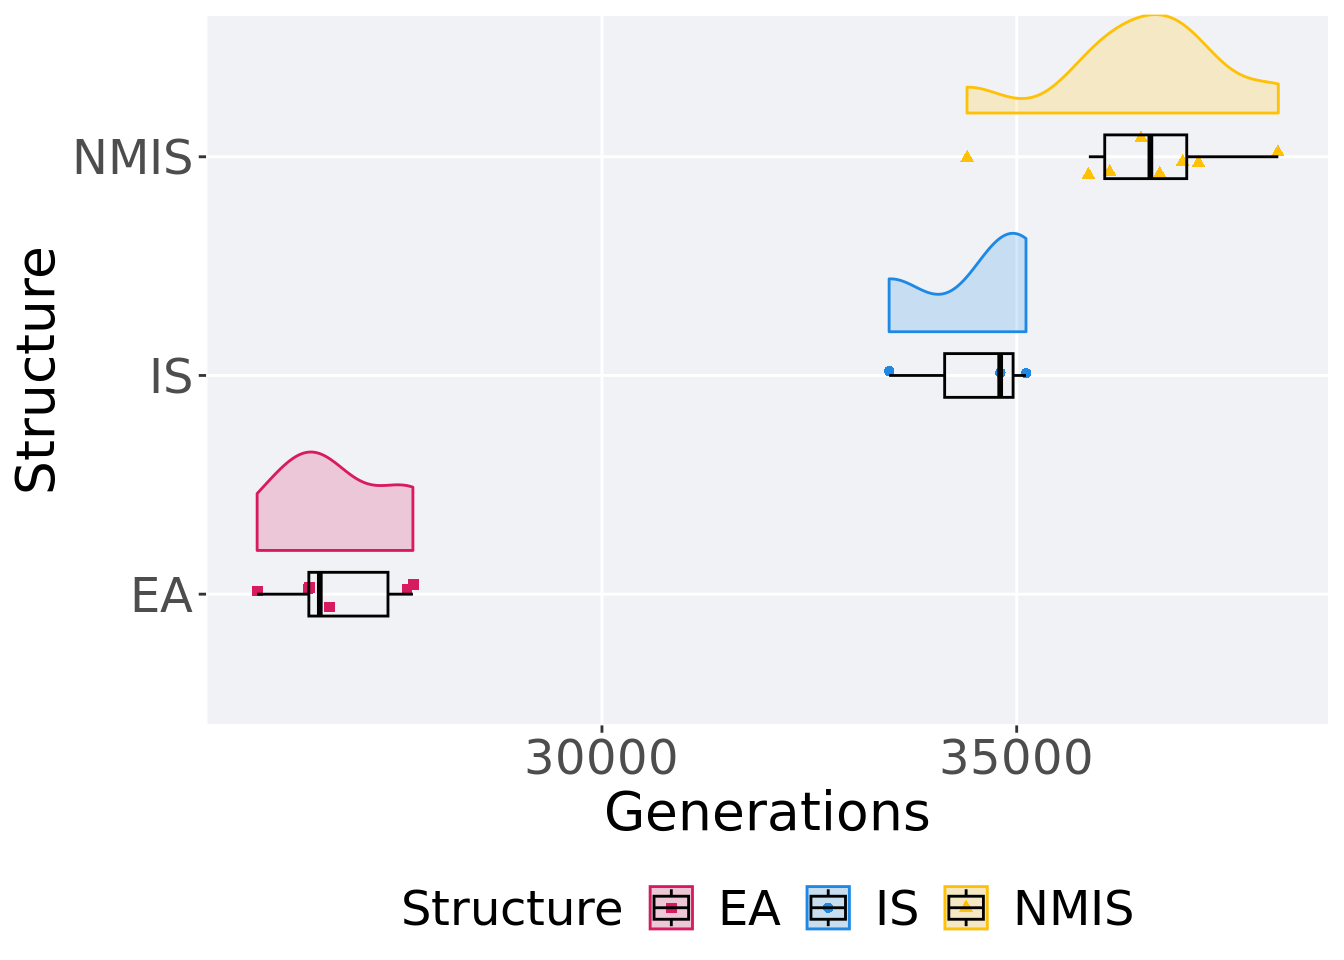
\includegraphics{demo_files/figure-latex/base-tor-mpe-ssf-1.pdf}

\hypertarget{stats-23}{%
\subsubsection{Stats}\label{stats-23}}

Summary statistics for the first generation a satisfactory solution is found.

\begin{Shaded}
\begin{Highlighting}[]
\NormalTok{ssf =}\StringTok{ }\KeywordTok{filter}\NormalTok{(base_ssf, Diagnostic }\OperatorTok{==}\StringTok{ 'MULTIPATH_EXPLORATION'} \OperatorTok{&}\StringTok{ `}\DataTypeTok{Selection}\CharTok{\textbackslash{}n}\DataTypeTok{Scheme}\StringTok{`} \OperatorTok{==}\StringTok{ 'TOURNAMENT'} \OperatorTok{&}\StringTok{ }\NormalTok{Generations }\OperatorTok{<}\StringTok{ }\DecValTok{60000}\NormalTok{)}
\NormalTok{ssf }\OperatorTok
\StringTok{  }\KeywordTok{group_by}\NormalTok{(Structure) }\OperatorTok
\StringTok{  }\NormalTok{dplyr}\OperatorTok{::}\KeywordTok{summarise}\NormalTok{(}
    \DataTypeTok{count =} \KeywordTok{n}\NormalTok{(),}
    \DataTypeTok{na_cnt =} \KeywordTok{sum}\NormalTok{(}\KeywordTok{is.na}\NormalTok{(Generations)),}
    \DataTypeTok{min =} \KeywordTok{min}\NormalTok{(Generations, }\DataTypeTok{na.rm =} \OtherTok{TRUE}\NormalTok{),}
    \DataTypeTok{median =} \KeywordTok{median}\NormalTok{(Generations, }\DataTypeTok{na.rm =} \OtherTok{TRUE}\NormalTok{),}
    \DataTypeTok{mean =} \KeywordTok{mean}\NormalTok{(Generations, }\DataTypeTok{na.rm =} \OtherTok{TRUE}\NormalTok{),}
    \DataTypeTok{max =} \KeywordTok{max}\NormalTok{(Generations, }\DataTypeTok{na.rm =} \OtherTok{TRUE}\NormalTok{),}
    \DataTypeTok{IQR =} \KeywordTok{IQR}\NormalTok{(Generations, }\DataTypeTok{na.rm =} \OtherTok{TRUE}\NormalTok{)}
\NormalTok{  )}
\end{Highlighting}
\end{Shaded}

\begin{verbatim}
## # A tibble: 3 x 8
##   Structure count na_cnt   min median   mean   max   IQR
##   <fct>     <int>  <int> <int>  <dbl>  <dbl> <int> <dbl>
## 1 EA            6      0 25843 26598. 26813  27721  954 
## 2 IS            3      0 33462 34801  34458. 35112  825 
## 3 NMIS          8      0 34401 36612. 36496. 38154  989.
\end{verbatim}

Kruskal--Wallis test provides evidence of no difference among selection schemes.

\begin{Shaded}
\begin{Highlighting}[]
\KeywordTok{kruskal.test}\NormalTok{(Generations }\OperatorTok{~}\StringTok{ }\NormalTok{Structure, }\DataTypeTok{data =}\NormalTok{ ssf)}
\end{Highlighting}
\end{Shaded}

\begin{verbatim}
## 
##  Kruskal-Wallis rank sum test
## 
## data:  Generations by Structure
## Kruskal-Wallis chi-squared = 12.797, df = 2, p-value = 0.001664
\end{verbatim}

\begin{Shaded}
\begin{Highlighting}[]
\KeywordTok{pairwise.wilcox.test}\NormalTok{(}\DataTypeTok{x =}\NormalTok{ ssf}\OperatorTok{$}\NormalTok{Generations, }\DataTypeTok{g =}\NormalTok{ ssf}\OperatorTok{$}\NormalTok{Structure, }\DataTypeTok{p.adjust.method =} \StringTok{"bonferroni"}\NormalTok{,}
                     \DataTypeTok{paired =} \OtherTok{FALSE}\NormalTok{, }\DataTypeTok{conf.int =} \OtherTok{FALSE}\NormalTok{, }\DataTypeTok{alternative =} \StringTok{'g'}\NormalTok{)}
\end{Highlighting}
\end{Shaded}

\begin{verbatim}
## 
##  Pairwise comparisons using Wilcoxon rank sum exact test 
## 
## data:  ssf$Generations and ssf$Structure 
## 
##      EA    IS   
## IS   0.036 -    
## NMIS 0.001 0.073
## 
## P value adjustment method: bonferroni
\end{verbatim}

\hypertarget{activation-gene-coverage-4}{%
\subsection{Activation gene coverage}\label{activation-gene-coverage-4}}

Activation gene coverage analysis.

\hypertarget{coverage-over-time-7}{%
\subsubsection{Coverage over time}\label{coverage-over-time-7}}

Activation gene coverage over time.

\begin{Shaded}
\begin{Highlighting}[]
\CommentTok{# data for lines and shading on plots}
\NormalTok{lines =}\StringTok{ }\KeywordTok{filter}\NormalTok{(base_over_time, Diagnostic }\OperatorTok{==}\StringTok{ 'MULTIPATH_EXPLORATION'} \OperatorTok{&}\StringTok{ `}\DataTypeTok{Selection}\CharTok{\textbackslash{}n}\DataTypeTok{Scheme}\StringTok{`} \OperatorTok{==}\StringTok{ 'TOURNAMENT'}\NormalTok{) }\OperatorTok
\StringTok{  }\KeywordTok{group_by}\NormalTok{(Structure, Generations) }\OperatorTok
\StringTok{  }\NormalTok{dplyr}\OperatorTok{::}\KeywordTok{summarise}\NormalTok{(}
    \DataTypeTok{min =} \KeywordTok{min}\NormalTok{(pop_act_cov),}
    \DataTypeTok{mean =} \KeywordTok{mean}\NormalTok{(pop_act_cov),}
    \DataTypeTok{max =} \KeywordTok{max}\NormalTok{(pop_act_cov)}
\NormalTok{  )}
\end{Highlighting}
\end{Shaded}

\begin{verbatim}
## `summarise()` has grouped output by 'Structure'. You can override using the
## `.groups` argument.
\end{verbatim}

\begin{Shaded}
\begin{Highlighting}[]
\KeywordTok{ggplot}\NormalTok{(lines, }\KeywordTok{aes}\NormalTok{(}\DataTypeTok{x=}\NormalTok{Generations, }\DataTypeTok{y=}\NormalTok{mean, }\DataTypeTok{group =}\NormalTok{ Structure, }\DataTypeTok{fill =}\NormalTok{ Structure, }\DataTypeTok{color =}\NormalTok{ Structure, }\DataTypeTok{shape =}\NormalTok{ Structure)) }\OperatorTok{+}
\StringTok{  }\KeywordTok{geom_ribbon}\NormalTok{(}\KeywordTok{aes}\NormalTok{(}\DataTypeTok{ymin =}\NormalTok{ min, }\DataTypeTok{ymax =}\NormalTok{ max), }\DataTypeTok{alpha =} \FloatTok{0.1}\NormalTok{) }\OperatorTok{+}
\StringTok{  }\KeywordTok{geom_line}\NormalTok{(}\DataTypeTok{size =} \FloatTok{0.5}\NormalTok{) }\OperatorTok{+}
\StringTok{  }\KeywordTok{geom_point}\NormalTok{(}\DataTypeTok{data =} \KeywordTok{filter}\NormalTok{(lines, Generations }\OperatorTok\StringTok{ }\DecValTok{2000} \OperatorTok{==}\StringTok{ }\DecValTok{0}\NormalTok{), }\DataTypeTok{size =} \FloatTok{1.5}\NormalTok{, }\DataTypeTok{stroke =} \FloatTok{2.0}\NormalTok{, }\DataTypeTok{alpha =} \FloatTok{1.0}\NormalTok{) }\OperatorTok{+}
\StringTok{  }\KeywordTok{scale_y_continuous}\NormalTok{(}
    \DataTypeTok{name=}\StringTok{"Coverage"}
\NormalTok{  ) }\OperatorTok{+}
\StringTok{  }\KeywordTok{scale_x_continuous}\NormalTok{(}
    \DataTypeTok{name=}\StringTok{"Generations"}\NormalTok{,}
    \DataTypeTok{limits=}\KeywordTok{c}\NormalTok{(}\DecValTok{0}\NormalTok{, }\DecValTok{50000}\NormalTok{),}
    \DataTypeTok{breaks=}\KeywordTok{c}\NormalTok{(}\DecValTok{0}\NormalTok{, }\DecValTok{10000}\NormalTok{, }\DecValTok{20000}\NormalTok{, }\DecValTok{30000}\NormalTok{, }\DecValTok{40000}\NormalTok{, }\DecValTok{50000}\NormalTok{),}
    \DataTypeTok{labels=}\KeywordTok{c}\NormalTok{(}\StringTok{"0e+4"}\NormalTok{, }\StringTok{"1e+4"}\NormalTok{, }\StringTok{"2e+4"}\NormalTok{, }\StringTok{"3e+4"}\NormalTok{, }\StringTok{"4e+4"}\NormalTok{, }\StringTok{"5e+4"}\NormalTok{)}

\NormalTok{  ) }\OperatorTok{+}
\StringTok{  }\KeywordTok{scale_shape_manual}\NormalTok{(}\DataTypeTok{values=}\NormalTok{SHAPE)}\OperatorTok{+}
\StringTok{  }\KeywordTok{scale_colour_manual}\NormalTok{(}\DataTypeTok{values =}\NormalTok{ cb_palette) }\OperatorTok{+}
\StringTok{  }\KeywordTok{scale_fill_manual}\NormalTok{(}\DataTypeTok{values =}\NormalTok{ cb_palette) }\OperatorTok{+}
\StringTok{  }\KeywordTok{ggtitle}\NormalTok{(}\StringTok{'Activation gene coverage over time'}\NormalTok{)}\OperatorTok{+}
\StringTok{  }\NormalTok{p_theme}
\end{Highlighting}
\end{Shaded}

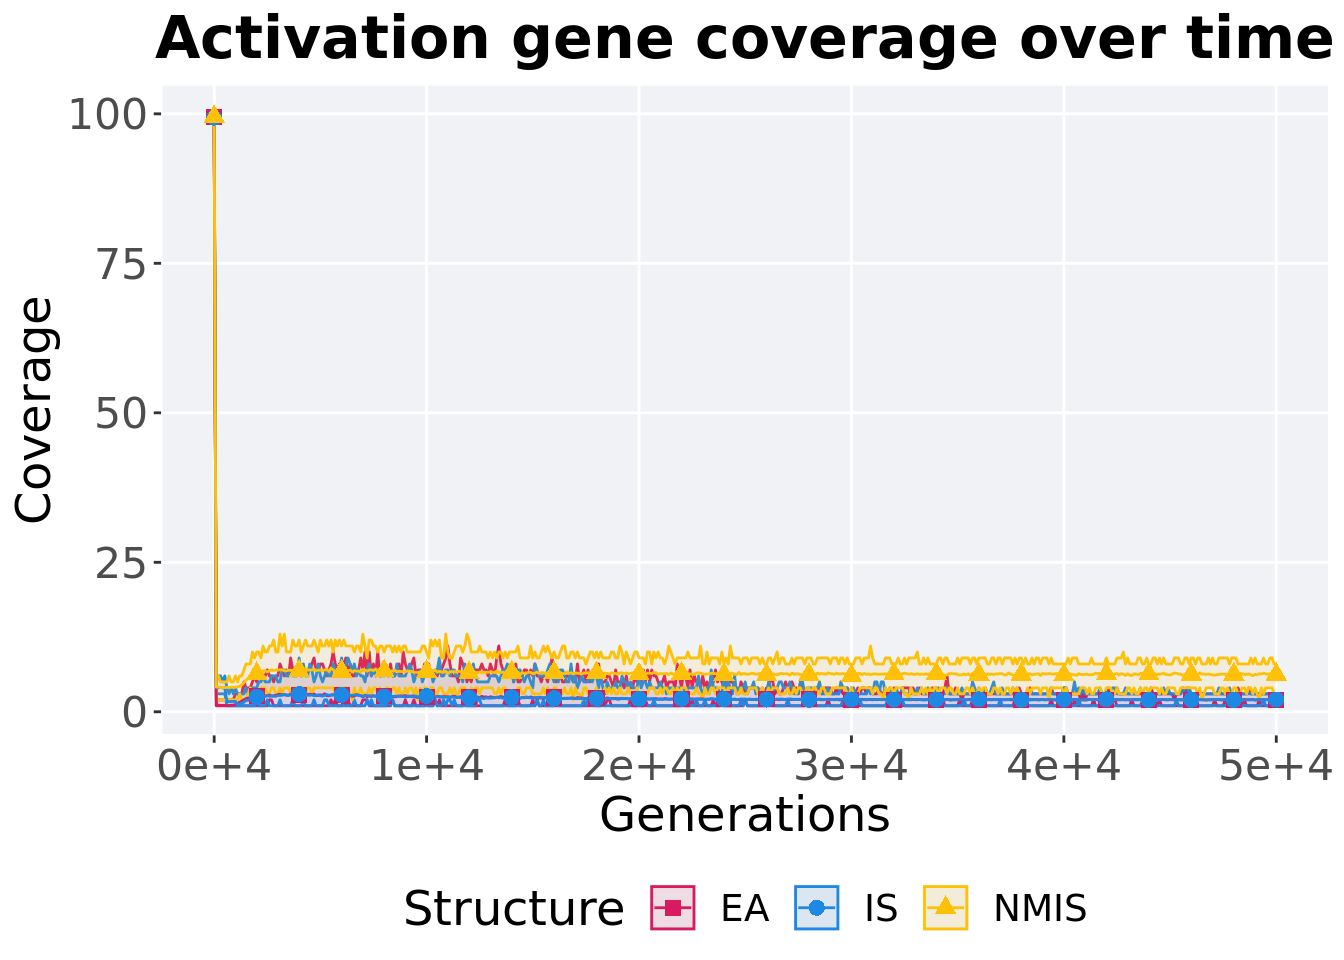
\includegraphics{demo_files/figure-latex/base-mpe-act-tor-ot-1.pdf}

\hypertarget{end-of-50000-generations-7}{%
\subsubsection{End of 50,000 generations}\label{end-of-50000-generations-7}}

Activation gene coverage in the population at the end of 50,000 generations.

\begin{Shaded}
\begin{Highlighting}[]
\CommentTok{### end of run}
\KeywordTok{filter}\NormalTok{(base_over_time, Diagnostic }\OperatorTok{==}\StringTok{ 'MULTIPATH_EXPLORATION'} \OperatorTok{&}\StringTok{ `}\DataTypeTok{Selection}\CharTok{\textbackslash{}n}\DataTypeTok{Scheme}\StringTok{`} \OperatorTok{==}\StringTok{ 'TOURNAMENT'} \OperatorTok{&}\StringTok{ }\NormalTok{Generations }\OperatorTok{==}\StringTok{ }\DecValTok{50000}\NormalTok{) }\OperatorTok
\StringTok{  }\KeywordTok{ggplot}\NormalTok{(., }\KeywordTok{aes}\NormalTok{(}\DataTypeTok{x =}\NormalTok{ Structure, }\DataTypeTok{y =}\NormalTok{ pop_act_cov, }\DataTypeTok{color =}\NormalTok{ Structure, }\DataTypeTok{fill =}\NormalTok{ Structure, }\DataTypeTok{shape =}\NormalTok{ Structure)) }\OperatorTok{+}
\StringTok{  }\KeywordTok{geom_flat_violin}\NormalTok{(}\DataTypeTok{position =} \KeywordTok{position_nudge}\NormalTok{(}\DataTypeTok{x =} \FloatTok{.2}\NormalTok{, }\DataTypeTok{y =} \DecValTok{0}\NormalTok{), }\DataTypeTok{scale =} \StringTok{'width'}\NormalTok{, }\DataTypeTok{alpha =} \FloatTok{0.3}\NormalTok{) }\OperatorTok{+}
\StringTok{  }\KeywordTok{geom_point}\NormalTok{(}\DataTypeTok{position =} \KeywordTok{position_jitter}\NormalTok{(}\DataTypeTok{height =} \FloatTok{.05}\NormalTok{, }\DataTypeTok{width =} \FloatTok{.05}\NormalTok{), }\DataTypeTok{size =} \FloatTok{1.5}\NormalTok{, }\DataTypeTok{alpha =} \FloatTok{0.5}\NormalTok{) }\OperatorTok{+}
\StringTok{  }\KeywordTok{geom_boxplot}\NormalTok{(}\DataTypeTok{color =} \StringTok{'black'}\NormalTok{, }\DataTypeTok{width =} \FloatTok{.2}\NormalTok{, }\DataTypeTok{outlier.shape =} \OtherTok{NA}\NormalTok{, }\DataTypeTok{alpha =} \FloatTok{0.0}\NormalTok{) }\OperatorTok{+}
\StringTok{  }\KeywordTok{scale_shape_manual}\NormalTok{(}\DataTypeTok{values=}\NormalTok{SHAPE)}\OperatorTok{+}
\StringTok{  }\KeywordTok{scale_y_continuous}\NormalTok{(}
    \DataTypeTok{name=}\StringTok{"Coverage"}
\NormalTok{  ) }\OperatorTok{+}
\StringTok{  }\KeywordTok{scale_x_discrete}\NormalTok{(}
    \DataTypeTok{name=}\StringTok{"Structure"}
\NormalTok{  ) }\OperatorTok{+}
\StringTok{  }\KeywordTok{scale_colour_manual}\NormalTok{(}\DataTypeTok{values =}\NormalTok{ cb_palette) }\OperatorTok{+}
\StringTok{  }\KeywordTok{scale_fill_manual}\NormalTok{(}\DataTypeTok{values =}\NormalTok{ cb_palette) }\OperatorTok{+}
\StringTok{  }\KeywordTok{ggtitle}\NormalTok{(}\StringTok{'Final activation gene coverage'}\NormalTok{)}\OperatorTok{+}
\StringTok{  }\NormalTok{p_theme }\OperatorTok{+}\StringTok{ }\KeywordTok{coord_flip}\NormalTok{()}
\end{Highlighting}
\end{Shaded}

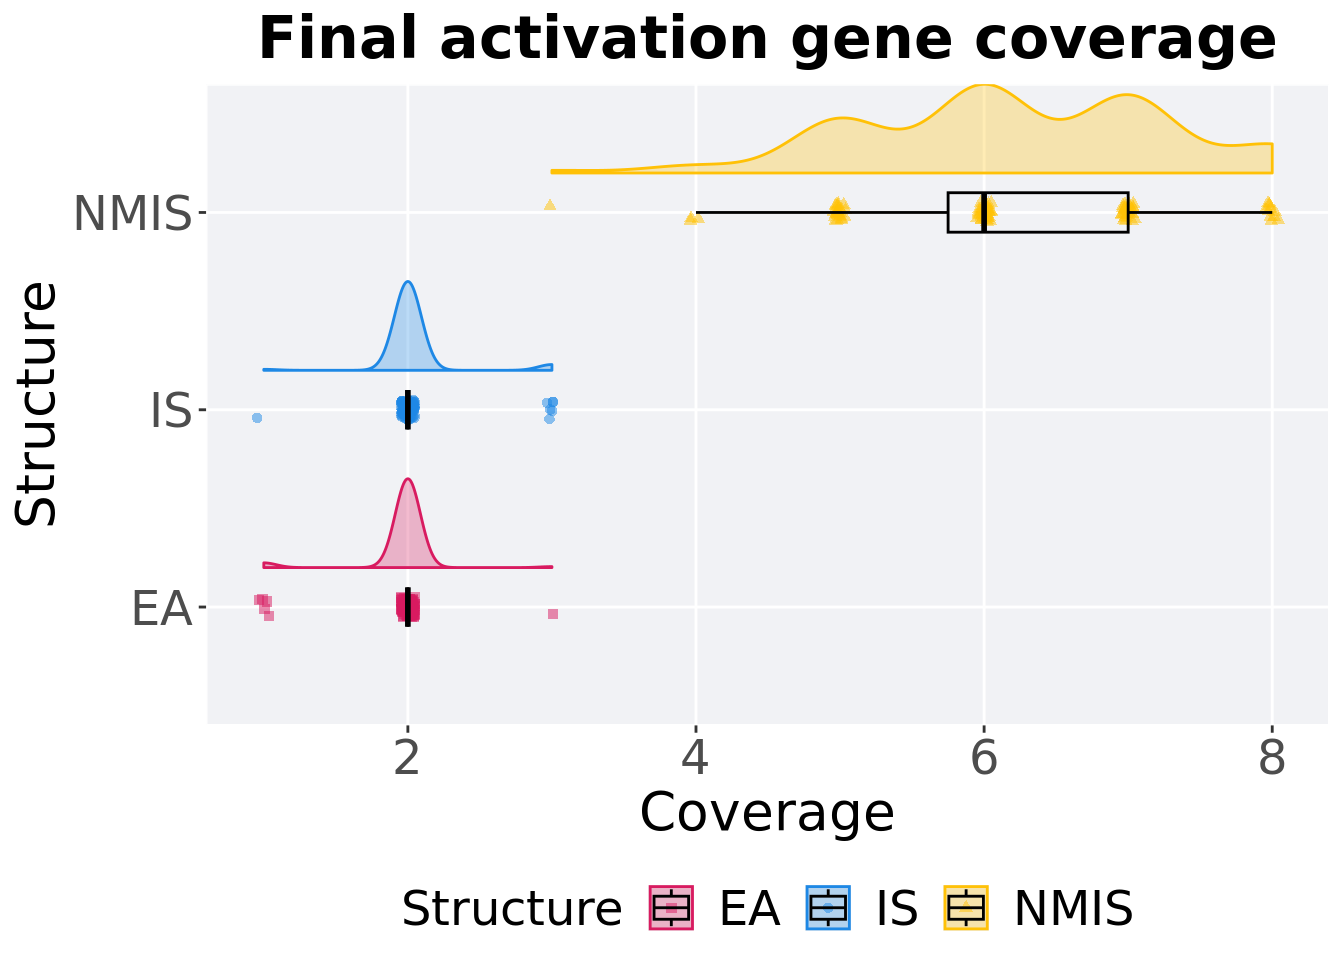
\includegraphics{demo_files/figure-latex/base-mpe-act-tor-end-1.pdf}

\hypertarget{stats-24}{%
\paragraph{Stats}\label{stats-24}}

Summary statistics for activation gene coverage.

\begin{Shaded}
\begin{Highlighting}[]
\NormalTok{coverage =}\StringTok{ }\KeywordTok{filter}\NormalTok{(base_over_time, Diagnostic }\OperatorTok{==}\StringTok{ 'MULTIPATH_EXPLORATION'} \OperatorTok{&}\StringTok{ `}\DataTypeTok{Selection}\CharTok{\textbackslash{}n}\DataTypeTok{Scheme}\StringTok{`} \OperatorTok{==}\StringTok{ 'TOURNAMENT'} \OperatorTok{&}\StringTok{ }\NormalTok{Generations }\OperatorTok{==}\StringTok{ }\DecValTok{50000}\NormalTok{)}
\NormalTok{coverage }\OperatorTok
\StringTok{  }\KeywordTok{group_by}\NormalTok{(Structure) }\OperatorTok
\StringTok{  }\NormalTok{dplyr}\OperatorTok{::}\KeywordTok{summarise}\NormalTok{(}
    \DataTypeTok{count =} \KeywordTok{n}\NormalTok{(),}
    \DataTypeTok{na_cnt =} \KeywordTok{sum}\NormalTok{(}\KeywordTok{is.na}\NormalTok{(pop_act_cov)),}
    \DataTypeTok{min =} \KeywordTok{min}\NormalTok{(pop_act_cov, }\DataTypeTok{na.rm =} \OtherTok{TRUE}\NormalTok{),}
    \DataTypeTok{median =} \KeywordTok{median}\NormalTok{(pop_act_cov, }\DataTypeTok{na.rm =} \OtherTok{TRUE}\NormalTok{),}
    \DataTypeTok{mean =} \KeywordTok{mean}\NormalTok{(pop_act_cov, }\DataTypeTok{na.rm =} \OtherTok{TRUE}\NormalTok{),}
    \DataTypeTok{max =} \KeywordTok{max}\NormalTok{(pop_act_cov, }\DataTypeTok{na.rm =} \OtherTok{TRUE}\NormalTok{),}
    \DataTypeTok{IQR =} \KeywordTok{IQR}\NormalTok{(pop_act_cov, }\DataTypeTok{na.rm =} \OtherTok{TRUE}\NormalTok{)}
\NormalTok{  )}
\end{Highlighting}
\end{Shaded}

\begin{verbatim}
## # A tibble: 3 x 8
##   Structure count na_cnt   min median  mean   max   IQR
##   <fct>     <int>  <int> <int>  <dbl> <dbl> <int> <dbl>
## 1 EA          100      0     1      2  1.96     3  0   
## 2 IS          100      0     1      2  2.05     3  0   
## 3 NMIS        100      0     3      6  6.22     8  1.25
\end{verbatim}

Kruskal--Wallis test provides evidence of difference among activation gene coverage.

\begin{Shaded}
\begin{Highlighting}[]
\KeywordTok{kruskal.test}\NormalTok{(pop_act_cov }\OperatorTok{~}\StringTok{ }\NormalTok{Structure, }\DataTypeTok{data =}\NormalTok{ coverage)}
\end{Highlighting}
\end{Shaded}

\begin{verbatim}
## 
##  Kruskal-Wallis rank sum test
## 
## data:  pop_act_cov by Structure
## Kruskal-Wallis chi-squared = 264.53, df = 2, p-value < 2.2e-16
\end{verbatim}

Results for post-hoc Wilcoxon rank-sum test with a Bonferroni correction on activation gene coverage.

\begin{Shaded}
\begin{Highlighting}[]
\KeywordTok{pairwise.wilcox.test}\NormalTok{(}\DataTypeTok{x =}\NormalTok{ coverage}\OperatorTok{$}\NormalTok{pop_act_cov, }\DataTypeTok{g =}\NormalTok{ coverage}\OperatorTok{$}\NormalTok{Structure, }\DataTypeTok{p.adjust.method =} \StringTok{"bonferroni"}\NormalTok{,}
                     \DataTypeTok{paired =} \OtherTok{FALSE}\NormalTok{, }\DataTypeTok{conf.int =} \OtherTok{FALSE}\NormalTok{, }\DataTypeTok{alternative =} \StringTok{'g'}\NormalTok{)}
\end{Highlighting}
\end{Shaded}

\begin{verbatim}
## 
##  Pairwise comparisons using Wilcoxon rank sum test with continuity correction 
## 
## data:  coverage$pop_act_cov and coverage$Structure 
## 
##      EA     IS    
## IS   0.019  -     
## NMIS <2e-16 <2e-16
## 
## P value adjustment method: bonferroni
\end{verbatim}

\hypertarget{lexicase-selection-3}{%
\section{Lexicase selection}\label{lexicase-selection-3}}

Here we analyze how the different population structures affect standard lexicase selection on the contradictory objectives diagnostic.

\hypertarget{performance-2}{%
\subsection{Performance}\label{performance-2}}

\hypertarget{performance-over-time-8}{%
\subsubsection{Performance over time}\label{performance-over-time-8}}

\begin{Shaded}
\begin{Highlighting}[]
\NormalTok{lines =}\StringTok{ }\KeywordTok{filter}\NormalTok{(base_over_time, Diagnostic }\OperatorTok{==}\StringTok{ 'MULTIPATH_EXPLORATION'} \OperatorTok{&}\StringTok{ `}\DataTypeTok{Selection}\CharTok{\textbackslash{}n}\DataTypeTok{Scheme}\StringTok{`} \OperatorTok{==}\StringTok{ 'LEXICASE'}\NormalTok{) }\OperatorTok
\StringTok{  }\KeywordTok{group_by}\NormalTok{(Structure, Generations) }\OperatorTok
\StringTok{  }\NormalTok{dplyr}\OperatorTok{::}\KeywordTok{summarise}\NormalTok{(}
    \DataTypeTok{min =} \KeywordTok{min}\NormalTok{(pop_fit_max) }\OperatorTok{/}\StringTok{ }\NormalTok{DIMENSIONALITY,}
    \DataTypeTok{mean =} \KeywordTok{mean}\NormalTok{(pop_fit_max) }\OperatorTok{/}\StringTok{ }\NormalTok{DIMENSIONALITY,}
    \DataTypeTok{max =} \KeywordTok{max}\NormalTok{(pop_fit_max) }\OperatorTok{/}\StringTok{ }\NormalTok{DIMENSIONALITY}
\NormalTok{  )}
\KeywordTok{ggplot}\NormalTok{(lines, }\KeywordTok{aes}\NormalTok{(}\DataTypeTok{x=}\NormalTok{Generations, }\DataTypeTok{y=}\NormalTok{mean, }\DataTypeTok{group =}\NormalTok{ Structure, }\DataTypeTok{fill =}\NormalTok{ Structure, }\DataTypeTok{color =}\NormalTok{ Structure, }\DataTypeTok{shape =}\NormalTok{ Structure)) }\OperatorTok{+}
\StringTok{  }\KeywordTok{geom_ribbon}\NormalTok{(}\KeywordTok{aes}\NormalTok{(}\DataTypeTok{ymin =}\NormalTok{ min, }\DataTypeTok{ymax =}\NormalTok{ max), }\DataTypeTok{alpha =} \FloatTok{0.1}\NormalTok{) }\OperatorTok{+}
\StringTok{  }\KeywordTok{geom_line}\NormalTok{(}\DataTypeTok{size =} \FloatTok{0.5}\NormalTok{) }\OperatorTok{+}
\StringTok{  }\KeywordTok{geom_point}\NormalTok{(}\DataTypeTok{data =} \KeywordTok{filter}\NormalTok{(lines, Generations }\OperatorTok\StringTok{ }\DecValTok{2000} \OperatorTok{==}\StringTok{ }\DecValTok{0}\NormalTok{), }\DataTypeTok{size =} \FloatTok{2.5}\NormalTok{, }\DataTypeTok{stroke =} \FloatTok{2.0}\NormalTok{, }\DataTypeTok{alpha =} \FloatTok{1.0}\NormalTok{) }\OperatorTok{+}
\StringTok{  }\KeywordTok{scale_y_continuous}\NormalTok{(}
    \DataTypeTok{name=}\StringTok{"Average trait score"}
\NormalTok{  ) }\OperatorTok{+}
\StringTok{  }\KeywordTok{scale_x_continuous}\NormalTok{(}
    \DataTypeTok{name=}\StringTok{"Generations"}\NormalTok{,}
    \DataTypeTok{limits=}\KeywordTok{c}\NormalTok{(}\DecValTok{0}\NormalTok{, }\DecValTok{50000}\NormalTok{),}
    \DataTypeTok{breaks=}\KeywordTok{c}\NormalTok{(}\DecValTok{0}\NormalTok{, }\DecValTok{10000}\NormalTok{, }\DecValTok{20000}\NormalTok{, }\DecValTok{30000}\NormalTok{, }\DecValTok{40000}\NormalTok{, }\DecValTok{50000}\NormalTok{),}
    \DataTypeTok{labels=}\KeywordTok{c}\NormalTok{(}\StringTok{"0e+4"}\NormalTok{, }\StringTok{"1e+4"}\NormalTok{, }\StringTok{"2e+4"}\NormalTok{, }\StringTok{"3e+4"}\NormalTok{, }\StringTok{"4e+4"}\NormalTok{, }\StringTok{"5e+4"}\NormalTok{)}

\NormalTok{  ) }\OperatorTok{+}
\StringTok{  }\KeywordTok{scale_shape_manual}\NormalTok{(}\DataTypeTok{values=}\NormalTok{SHAPE)}\OperatorTok{+}
\StringTok{  }\KeywordTok{scale_colour_manual}\NormalTok{(}\DataTypeTok{values =}\NormalTok{ cb_palette) }\OperatorTok{+}
\StringTok{  }\KeywordTok{scale_fill_manual}\NormalTok{(}\DataTypeTok{values =}\NormalTok{ cb_palette) }\OperatorTok{+}
\StringTok{  }\KeywordTok{ggtitle}\NormalTok{(}\StringTok{"Performance over time"}\NormalTok{) }\OperatorTok{+}
\StringTok{  }\NormalTok{p_theme}
\end{Highlighting}
\end{Shaded}

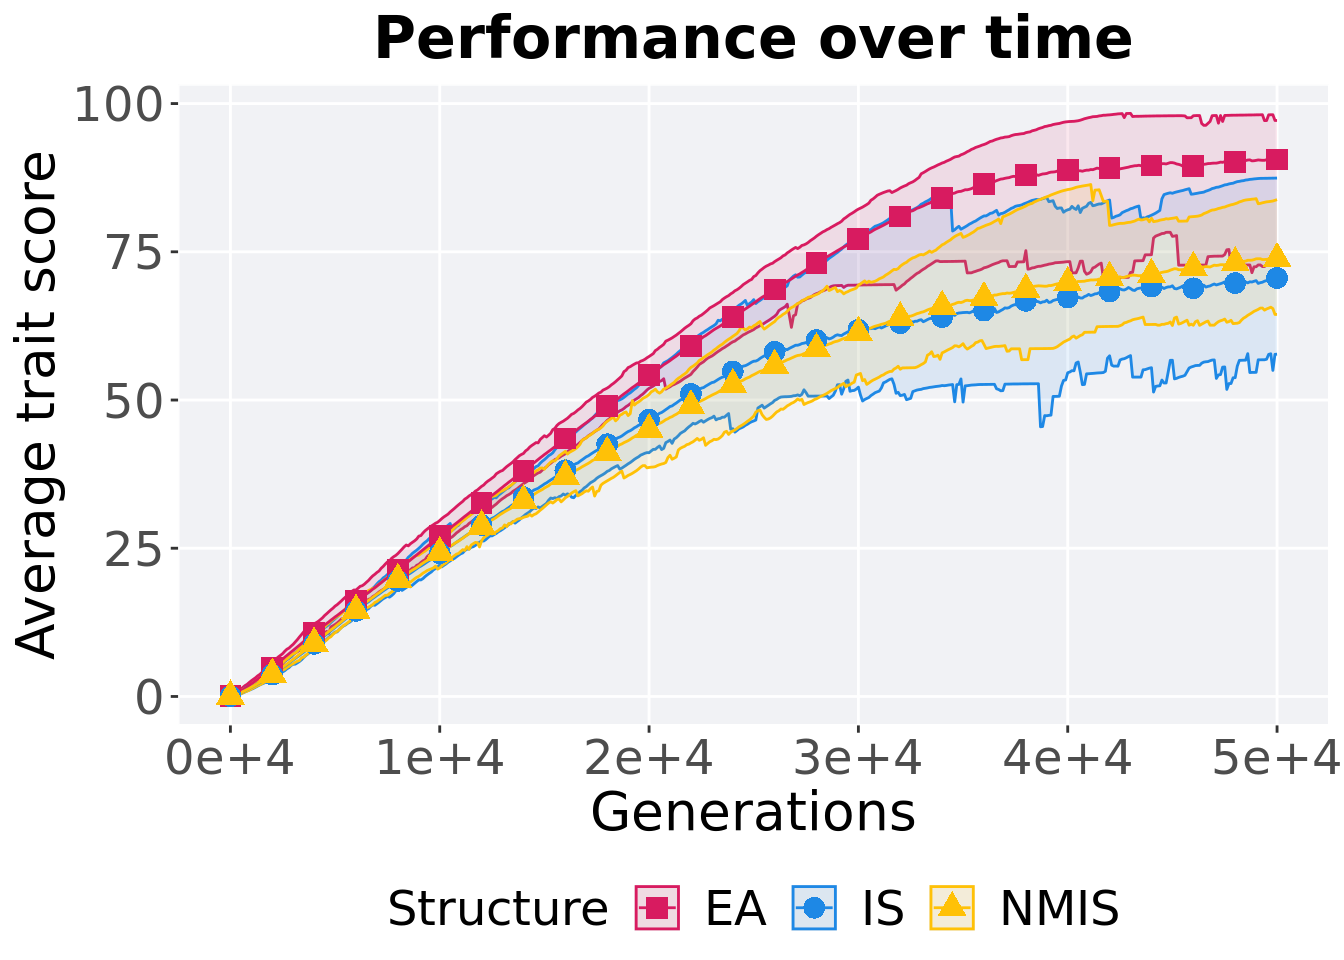
\includegraphics{demo_files/figure-latex/base-lex-mpe-perf-1.pdf}

\hypertarget{best-performance-3}{%
\subsubsection{Best performance}\label{best-performance-3}}

First generation a satisfactory solution is found throughout the 50,000 generations.

\begin{Shaded}
\begin{Highlighting}[]
\KeywordTok{filter}\NormalTok{(base_best, Diagnostic }\OperatorTok{==}\StringTok{ 'MULTIPATH_EXPLORATION'} \OperatorTok{&}\StringTok{ `}\DataTypeTok{Selection}\CharTok{\textbackslash{}n}\DataTypeTok{Scheme}\StringTok{`} \OperatorTok{==}\StringTok{ 'LEXICASE'} \OperatorTok{&}\StringTok{ }\NormalTok{VAR }\OperatorTok{==}\StringTok{ 'pop_fit_max'}\NormalTok{) }\OperatorTok
\StringTok{  }\KeywordTok{ggplot}\NormalTok{(., }\KeywordTok{aes}\NormalTok{(}\DataTypeTok{x =}\NormalTok{ Structure, }\DataTypeTok{y =}\NormalTok{ VAL }\OperatorTok{/}\StringTok{ }\NormalTok{DIMENSIONALITY, }\DataTypeTok{color =}\NormalTok{ Structure, }\DataTypeTok{fill =}\NormalTok{ Structure, }\DataTypeTok{shape =}\NormalTok{ Structure)) }\OperatorTok{+}
\StringTok{  }\KeywordTok{geom_flat_violin}\NormalTok{(}\DataTypeTok{position =} \KeywordTok{position_nudge}\NormalTok{(}\DataTypeTok{x =} \FloatTok{.2}\NormalTok{, }\DataTypeTok{y =} \DecValTok{0}\NormalTok{), }\DataTypeTok{scale =} \StringTok{'width'}\NormalTok{, }\DataTypeTok{alpha =} \FloatTok{0.2}\NormalTok{) }\OperatorTok{+}
\StringTok{  }\KeywordTok{geom_point}\NormalTok{(}\DataTypeTok{position =} \KeywordTok{position_jitter}\NormalTok{(}\DataTypeTok{width =} \FloatTok{.1}\NormalTok{), }\DataTypeTok{size =} \FloatTok{1.5}\NormalTok{, }\DataTypeTok{alpha =} \FloatTok{1.0}\NormalTok{) }\OperatorTok{+}
\StringTok{  }\KeywordTok{geom_boxplot}\NormalTok{(}\DataTypeTok{color =} \StringTok{'black'}\NormalTok{, }\DataTypeTok{width =} \FloatTok{.2}\NormalTok{, }\DataTypeTok{outlier.shape =} \OtherTok{NA}\NormalTok{, }\DataTypeTok{alpha =} \FloatTok{0.0}\NormalTok{) }\OperatorTok{+}
\StringTok{  }\KeywordTok{scale_y_continuous}\NormalTok{(}
    \DataTypeTok{name=}\StringTok{"Average trait score"}
\NormalTok{  ) }\OperatorTok{+}
\StringTok{  }\KeywordTok{scale_x_discrete}\NormalTok{(}
    \DataTypeTok{name=}\StringTok{"Structure"}
\NormalTok{  )}\OperatorTok{+}
\StringTok{  }\KeywordTok{scale_shape_manual}\NormalTok{(}\DataTypeTok{values=}\NormalTok{SHAPE)}\OperatorTok{+}
\StringTok{  }\KeywordTok{scale_colour_manual}\NormalTok{(}\DataTypeTok{values =}\NormalTok{ cb_palette, ) }\OperatorTok{+}
\StringTok{  }\KeywordTok{scale_fill_manual}\NormalTok{(}\DataTypeTok{values =}\NormalTok{ cb_palette) }\OperatorTok{+}
\StringTok{  }\KeywordTok{ggtitle}\NormalTok{(}\StringTok{'Best performance'}\NormalTok{)}\OperatorTok{+}
\StringTok{  }\NormalTok{p_theme }\OperatorTok{+}\StringTok{ }\KeywordTok{coord_flip}\NormalTok{()}
\end{Highlighting}
\end{Shaded}

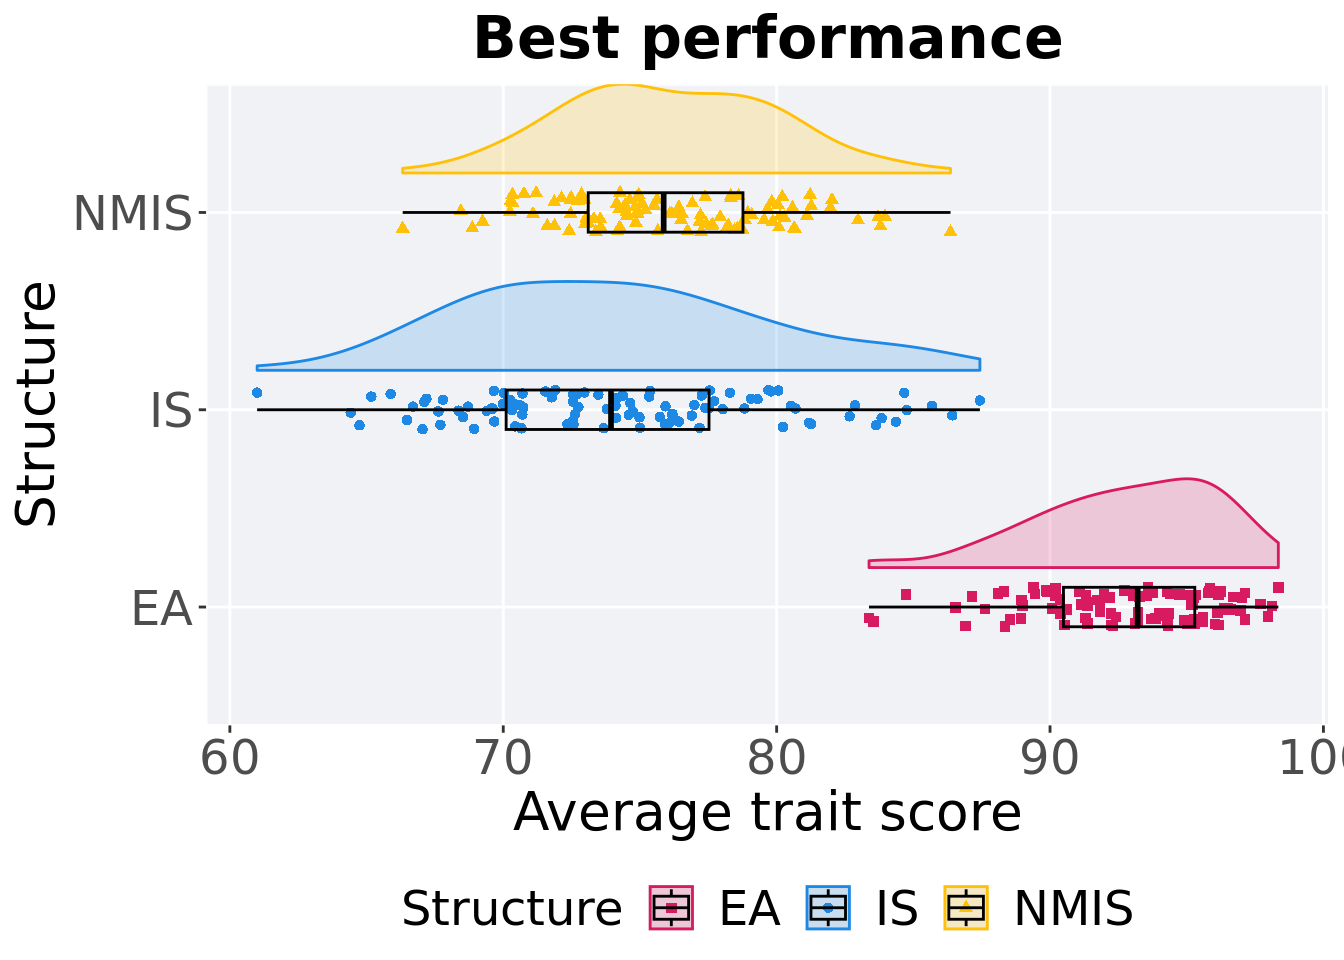
\includegraphics{demo_files/figure-latex/base-lex-mpe-per-bst-1.pdf}

\hypertarget{stats-25}{%
\paragraph{Stats}\label{stats-25}}

Summary statistics for the first generation a satisfactory solution is found.

\begin{Shaded}
\begin{Highlighting}[]
\NormalTok{performance =}\StringTok{ }\KeywordTok{filter}\NormalTok{(base_best, Diagnostic }\OperatorTok{==}\StringTok{ 'MULTIPATH_EXPLORATION'} \OperatorTok{&}\StringTok{ `}\DataTypeTok{Selection}\CharTok{\textbackslash{}n}\DataTypeTok{Scheme}\StringTok{`} \OperatorTok{==}\StringTok{ 'LEXICASE'} \OperatorTok{&}\StringTok{ }\NormalTok{VAR }\OperatorTok{==}\StringTok{ 'pop_fit_max'}\NormalTok{)}
\NormalTok{performance}\OperatorTok{$}\NormalTok{Structure =}\StringTok{ }\KeywordTok{factor}\NormalTok{(performance}\OperatorTok{$}\NormalTok{Structure, }\DataTypeTok{levels=}\KeywordTok{c}\NormalTok{(}\StringTok{'EA'}\NormalTok{,}\StringTok{'NMIS'}\NormalTok{,}\StringTok{'IS'}\NormalTok{))}
\NormalTok{performance }\OperatorTok
\StringTok{  }\KeywordTok{group_by}\NormalTok{(Structure) }\OperatorTok
\StringTok{  }\NormalTok{dplyr}\OperatorTok{::}\KeywordTok{summarise}\NormalTok{(}
    \DataTypeTok{count =} \KeywordTok{n}\NormalTok{(),}
    \DataTypeTok{na_cnt =} \KeywordTok{sum}\NormalTok{(}\KeywordTok{is.na}\NormalTok{(VAL)),}
    \DataTypeTok{min =} \KeywordTok{min}\NormalTok{(VAL, }\DataTypeTok{na.rm =} \OtherTok{TRUE}\NormalTok{) }\OperatorTok{/}\StringTok{ }\NormalTok{DIMENSIONALITY,}
    \DataTypeTok{median =} \KeywordTok{median}\NormalTok{(VAL, }\DataTypeTok{na.rm =} \OtherTok{TRUE}\NormalTok{) }\OperatorTok{/}\StringTok{ }\NormalTok{DIMENSIONALITY,}
    \DataTypeTok{mean =} \KeywordTok{mean}\NormalTok{(VAL, }\DataTypeTok{na.rm =} \OtherTok{TRUE}\NormalTok{) }\OperatorTok{/}\StringTok{ }\NormalTok{DIMENSIONALITY,}
    \DataTypeTok{max =} \KeywordTok{max}\NormalTok{(VAL, }\DataTypeTok{na.rm =} \OtherTok{TRUE}\NormalTok{) }\OperatorTok{/}\StringTok{ }\NormalTok{DIMENSIONALITY,}
    \DataTypeTok{IQR =} \KeywordTok{IQR}\NormalTok{(VAL, }\DataTypeTok{na.rm =} \OtherTok{TRUE}\NormalTok{) }\OperatorTok{/}\StringTok{ }\NormalTok{DIMENSIONALITY}
\NormalTok{  )}
\end{Highlighting}
\end{Shaded}

\begin{verbatim}
## # A tibble: 3 x 8
##   Structure count na_cnt   min median  mean   max   IQR
##   <fct>     <int>  <int> <dbl>  <dbl> <dbl> <dbl> <dbl>
## 1 EA          100      0  83.4   93.2  92.8  98.4  4.80
## 2 NMIS        100      0  66.3   75.9  76.1  86.4  5.66
## 3 IS          100      0  61.0   73.9  74.1  87.4  7.42
\end{verbatim}

Kruskal--Wallis test provides evidence of difference among selection schemes.

\begin{Shaded}
\begin{Highlighting}[]
\KeywordTok{kruskal.test}\NormalTok{(VAL }\OperatorTok{~}\StringTok{ }\NormalTok{Structure, }\DataTypeTok{data =}\NormalTok{ performance)}
\end{Highlighting}
\end{Shaded}

\begin{verbatim}
## 
##  Kruskal-Wallis rank sum test
## 
## data:  VAL by Structure
## Kruskal-Wallis chi-squared = 202.16, df = 2, p-value < 2.2e-16
\end{verbatim}

Results for post-hoc Wilcoxon rank-sum test with a Bonferroni correction.

\begin{Shaded}
\begin{Highlighting}[]
\KeywordTok{pairwise.wilcox.test}\NormalTok{(}\DataTypeTok{x =}\NormalTok{ performance}\OperatorTok{$}\NormalTok{VAL, }\DataTypeTok{g =}\NormalTok{ performance}\OperatorTok{$}\NormalTok{Structure, }\DataTypeTok{p.adjust.method =} \StringTok{"bonferroni"}\NormalTok{,}
                     \DataTypeTok{paired =} \OtherTok{FALSE}\NormalTok{, }\DataTypeTok{conf.int =} \OtherTok{FALSE}\NormalTok{, }\DataTypeTok{alternative =} \StringTok{'l'}\NormalTok{)}
\end{Highlighting}
\end{Shaded}

\begin{verbatim}
## 
##  Pairwise comparisons using Wilcoxon rank sum test with continuity correction 
## 
## data:  performance$VAL and performance$Structure 
## 
##      EA     NMIS  
## NMIS <2e-16 -     
## IS   <2e-16 0.0032
## 
## P value adjustment method: bonferroni
\end{verbatim}

\hypertarget{final-performance-3}{%
\subsubsection{Final performance}\label{final-performance-3}}

First generation a satisfactory solution is found throughout the 50,000 generations.

\begin{Shaded}
\begin{Highlighting}[]
\KeywordTok{filter}\NormalTok{(base_over_time, Diagnostic }\OperatorTok{==}\StringTok{ 'MULTIPATH_EXPLORATION'} \OperatorTok{&}\StringTok{ `}\DataTypeTok{Selection}\CharTok{\textbackslash{}n}\DataTypeTok{Scheme}\StringTok{`} \OperatorTok{==}\StringTok{ 'LEXICASE'} \OperatorTok{&}\StringTok{ }\NormalTok{Generations }\OperatorTok{==}\StringTok{ }\DecValTok{50000}\NormalTok{) }\OperatorTok
\StringTok{  }\KeywordTok{ggplot}\NormalTok{(., }\KeywordTok{aes}\NormalTok{(}\DataTypeTok{x =}\NormalTok{ Structure, }\DataTypeTok{y =}\NormalTok{ pop_fit_max }\OperatorTok{/}\StringTok{ }\NormalTok{DIMENSIONALITY, }\DataTypeTok{color =}\NormalTok{ Structure, }\DataTypeTok{fill =}\NormalTok{ Structure, }\DataTypeTok{shape =}\NormalTok{ Structure)) }\OperatorTok{+}
\StringTok{  }\KeywordTok{geom_flat_violin}\NormalTok{(}\DataTypeTok{position =} \KeywordTok{position_nudge}\NormalTok{(}\DataTypeTok{x =} \FloatTok{.2}\NormalTok{, }\DataTypeTok{y =} \DecValTok{0}\NormalTok{), }\DataTypeTok{scale =} \StringTok{'width'}\NormalTok{, }\DataTypeTok{alpha =} \FloatTok{0.2}\NormalTok{) }\OperatorTok{+}
\StringTok{  }\KeywordTok{geom_point}\NormalTok{(}\DataTypeTok{position =} \KeywordTok{position_jitter}\NormalTok{(}\DataTypeTok{width =} \FloatTok{.1}\NormalTok{), }\DataTypeTok{size =} \FloatTok{1.5}\NormalTok{, }\DataTypeTok{alpha =} \FloatTok{1.0}\NormalTok{) }\OperatorTok{+}
\StringTok{  }\KeywordTok{geom_boxplot}\NormalTok{(}\DataTypeTok{color =} \StringTok{'black'}\NormalTok{, }\DataTypeTok{width =} \FloatTok{.2}\NormalTok{, }\DataTypeTok{outlier.shape =} \OtherTok{NA}\NormalTok{, }\DataTypeTok{alpha =} \FloatTok{0.0}\NormalTok{) }\OperatorTok{+}
\StringTok{  }\KeywordTok{scale_y_continuous}\NormalTok{(}
    \DataTypeTok{name=}\StringTok{"Average trait score"}
\NormalTok{  ) }\OperatorTok{+}
\StringTok{  }\KeywordTok{scale_x_discrete}\NormalTok{(}
    \DataTypeTok{name=}\StringTok{"Structure"}
\NormalTok{  )}\OperatorTok{+}
\StringTok{  }\KeywordTok{scale_shape_manual}\NormalTok{(}\DataTypeTok{values=}\NormalTok{SHAPE)}\OperatorTok{+}
\StringTok{  }\KeywordTok{scale_colour_manual}\NormalTok{(}\DataTypeTok{values =}\NormalTok{ cb_palette, ) }\OperatorTok{+}
\StringTok{  }\KeywordTok{scale_fill_manual}\NormalTok{(}\DataTypeTok{values =}\NormalTok{ cb_palette) }\OperatorTok{+}
\StringTok{  }\KeywordTok{ggtitle}\NormalTok{(}\StringTok{'Final performance'}\NormalTok{)}\OperatorTok{+}
\StringTok{  }\NormalTok{p_theme }\OperatorTok{+}\StringTok{ }\KeywordTok{coord_flip}\NormalTok{()}
\end{Highlighting}
\end{Shaded}

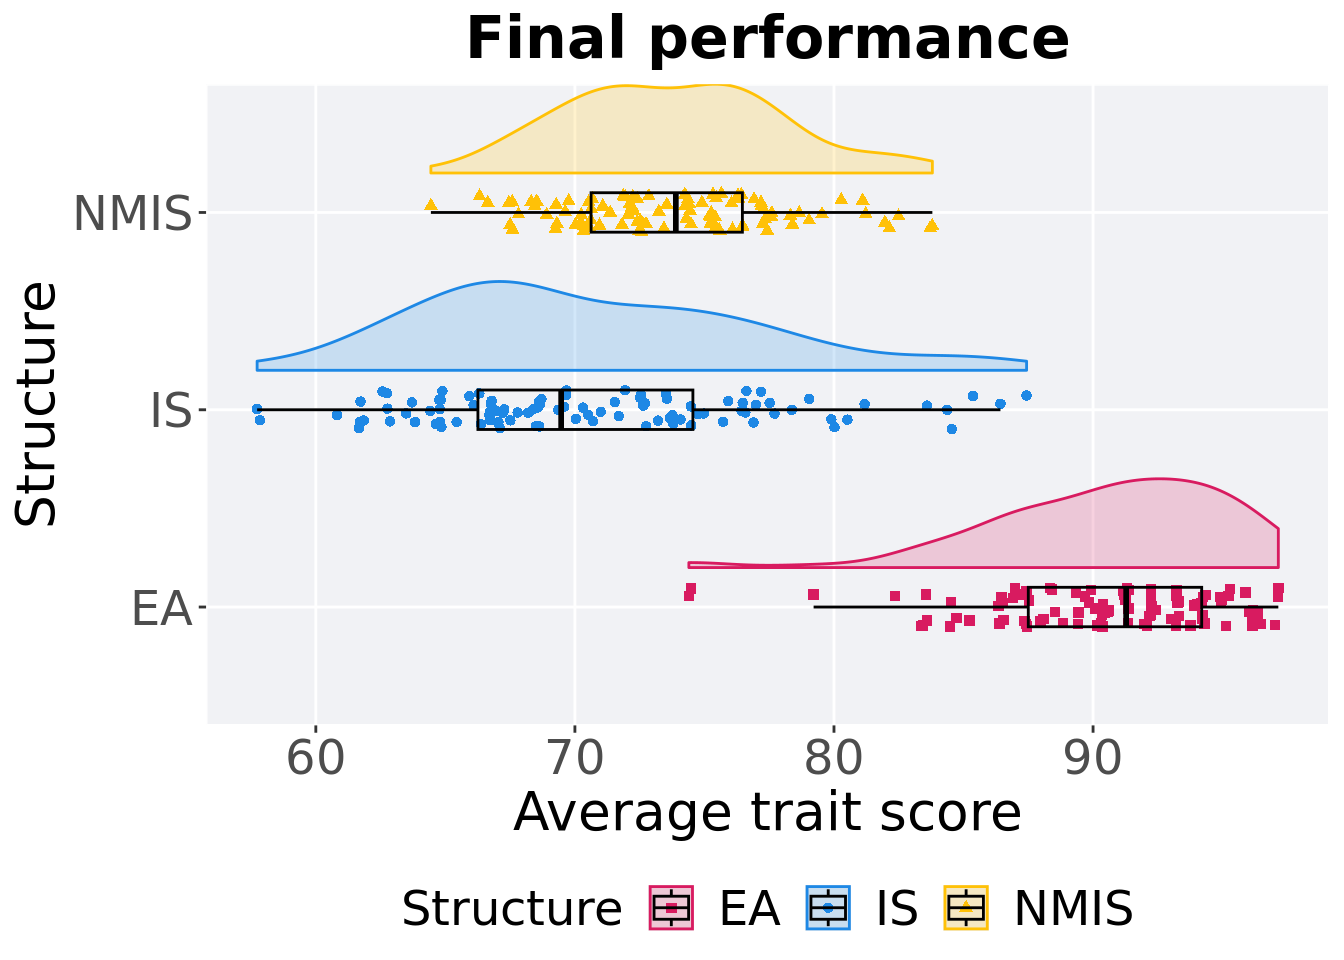
\includegraphics{demo_files/figure-latex/base-lex-mpe-per-end-1.pdf}

\hypertarget{stats-26}{%
\paragraph{Stats}\label{stats-26}}

Summary statistics for the first generation a satisfactory solution is found.

\begin{Shaded}
\begin{Highlighting}[]
\NormalTok{performance =}\StringTok{ }\KeywordTok{filter}\NormalTok{(base_over_time, Diagnostic }\OperatorTok{==}\StringTok{ 'MULTIPATH_EXPLORATION'} \OperatorTok{&}\StringTok{ `}\DataTypeTok{Selection}\CharTok{\textbackslash{}n}\DataTypeTok{Scheme}\StringTok{`} \OperatorTok{==}\StringTok{ 'LEXICASE'} \OperatorTok{&}\StringTok{ }\NormalTok{Generations }\OperatorTok{==}\StringTok{ }\DecValTok{50000}\NormalTok{)}
\NormalTok{performance}\OperatorTok{$}\NormalTok{Structure =}\StringTok{ }\KeywordTok{factor}\NormalTok{(performance}\OperatorTok{$}\NormalTok{Structure, }\DataTypeTok{levels=}\KeywordTok{c}\NormalTok{(}\StringTok{'EA'}\NormalTok{,}\StringTok{'NMIS'}\NormalTok{,}\StringTok{'IS'}\NormalTok{))}
\NormalTok{performance }\OperatorTok
\StringTok{  }\KeywordTok{group_by}\NormalTok{(Structure) }\OperatorTok
\StringTok{  }\NormalTok{dplyr}\OperatorTok{::}\KeywordTok{summarise}\NormalTok{(}
    \DataTypeTok{count =} \KeywordTok{n}\NormalTok{(),}
    \DataTypeTok{na_cnt =} \KeywordTok{sum}\NormalTok{(}\KeywordTok{is.na}\NormalTok{(pop_fit_max)),}
    \DataTypeTok{min =} \KeywordTok{min}\NormalTok{(pop_fit_max }\OperatorTok{/}\StringTok{ }\NormalTok{DIMENSIONALITY, }\DataTypeTok{na.rm =} \OtherTok{TRUE}\NormalTok{),}
    \DataTypeTok{median =} \KeywordTok{median}\NormalTok{(pop_fit_max }\OperatorTok{/}\StringTok{ }\NormalTok{DIMENSIONALITY, }\DataTypeTok{na.rm =} \OtherTok{TRUE}\NormalTok{),}
    \DataTypeTok{mean =} \KeywordTok{mean}\NormalTok{(pop_fit_max }\OperatorTok{/}\StringTok{ }\NormalTok{DIMENSIONALITY, }\DataTypeTok{na.rm =} \OtherTok{TRUE}\NormalTok{),}
    \DataTypeTok{max =} \KeywordTok{max}\NormalTok{(pop_fit_max }\OperatorTok{/}\StringTok{ }\NormalTok{DIMENSIONALITY, }\DataTypeTok{na.rm =} \OtherTok{TRUE}\NormalTok{),}
    \DataTypeTok{IQR =} \KeywordTok{IQR}\NormalTok{(pop_fit_max }\OperatorTok{/}\StringTok{ }\NormalTok{DIMENSIONALITY, }\DataTypeTok{na.rm =} \OtherTok{TRUE}\NormalTok{)}
\NormalTok{  )}
\end{Highlighting}
\end{Shaded}

\begin{verbatim}
## # A tibble: 3 x 8
##   Structure count na_cnt   min median  mean   max   IQR
##   <fct>     <int>  <int> <dbl>  <dbl> <dbl> <dbl> <dbl>
## 1 EA          100      0  74.4   91.3  90.6  97.2  6.69
## 2 NMIS        100      0  64.4   73.9  73.8  83.8  5.84
## 3 IS          100      0  57.7   69.5  70.6  87.4  8.30
\end{verbatim}

Kruskal--Wallis test provides evidence of difference among selection schemes.

\begin{Shaded}
\begin{Highlighting}[]
\KeywordTok{kruskal.test}\NormalTok{(pop_fit_max }\OperatorTok{~}\StringTok{ }\NormalTok{Structure, }\DataTypeTok{data =}\NormalTok{ performance)}
\end{Highlighting}
\end{Shaded}

\begin{verbatim}
## 
##  Kruskal-Wallis rank sum test
## 
## data:  pop_fit_max by Structure
## Kruskal-Wallis chi-squared = 198.85, df = 2, p-value < 2.2e-16
\end{verbatim}

Results for post-hoc Wilcoxon rank-sum test with a Bonferroni correction.

\begin{Shaded}
\begin{Highlighting}[]
\KeywordTok{pairwise.wilcox.test}\NormalTok{(}\DataTypeTok{x =}\NormalTok{ performance}\OperatorTok{$}\NormalTok{pop_fit_max, }\DataTypeTok{g =}\NormalTok{ performance}\OperatorTok{$}\NormalTok{Structure, }\DataTypeTok{p.adjust.method =} \StringTok{"bonferroni"}\NormalTok{,}
                     \DataTypeTok{paired =} \OtherTok{FALSE}\NormalTok{, }\DataTypeTok{conf.int =} \OtherTok{FALSE}\NormalTok{, }\DataTypeTok{alternative =} \StringTok{'l'}\NormalTok{)}
\end{Highlighting}
\end{Shaded}

\begin{verbatim}
## 
##  Pairwise comparisons using Wilcoxon rank sum test with continuity correction 
## 
## data:  performance$pop_fit_max and performance$Structure 
## 
##      EA      NMIS   
## NMIS < 2e-16 -      
## IS   < 2e-16 1.6e-05
## 
## P value adjustment method: bonferroni
\end{verbatim}

\hypertarget{activation-gene-coverage-5}{%
\subsection{Activation gene coverage}\label{activation-gene-coverage-5}}

Activation gene coverage analysis.

\hypertarget{coverage-over-time-8}{%
\subsubsection{Coverage over time}\label{coverage-over-time-8}}

Activation gene coverage over time.

\begin{Shaded}
\begin{Highlighting}[]
\CommentTok{# data for lines and shading on plots}
\NormalTok{lines =}\StringTok{ }\KeywordTok{filter}\NormalTok{(base_over_time, Diagnostic }\OperatorTok{==}\StringTok{ 'MULTIPATH_EXPLORATION'} \OperatorTok{&}\StringTok{ `}\DataTypeTok{Selection}\CharTok{\textbackslash{}n}\DataTypeTok{Scheme}\StringTok{`} \OperatorTok{==}\StringTok{ 'LEXICASE'}\NormalTok{) }\OperatorTok
\StringTok{  }\KeywordTok{group_by}\NormalTok{(Structure, Generations) }\OperatorTok
\StringTok{  }\NormalTok{dplyr}\OperatorTok{::}\KeywordTok{summarise}\NormalTok{(}
    \DataTypeTok{min =} \KeywordTok{min}\NormalTok{(pop_act_cov),}
    \DataTypeTok{mean =} \KeywordTok{mean}\NormalTok{(pop_act_cov),}
    \DataTypeTok{max =} \KeywordTok{max}\NormalTok{(pop_act_cov)}
\NormalTok{  )}
\end{Highlighting}
\end{Shaded}

\begin{verbatim}
## `summarise()` has grouped output by 'Structure'. You can override using the
## `.groups` argument.
\end{verbatim}

\begin{Shaded}
\begin{Highlighting}[]
\KeywordTok{ggplot}\NormalTok{(lines, }\KeywordTok{aes}\NormalTok{(}\DataTypeTok{x=}\NormalTok{Generations, }\DataTypeTok{y=}\NormalTok{mean, }\DataTypeTok{group =}\NormalTok{ Structure, }\DataTypeTok{fill =}\NormalTok{ Structure, }\DataTypeTok{color =}\NormalTok{ Structure, }\DataTypeTok{shape =}\NormalTok{ Structure)) }\OperatorTok{+}
\StringTok{  }\KeywordTok{geom_ribbon}\NormalTok{(}\KeywordTok{aes}\NormalTok{(}\DataTypeTok{ymin =}\NormalTok{ min, }\DataTypeTok{ymax =}\NormalTok{ max), }\DataTypeTok{alpha =} \FloatTok{0.1}\NormalTok{) }\OperatorTok{+}
\StringTok{  }\KeywordTok{geom_line}\NormalTok{(}\DataTypeTok{size =} \FloatTok{0.5}\NormalTok{) }\OperatorTok{+}
\StringTok{  }\KeywordTok{geom_point}\NormalTok{(}\DataTypeTok{data =} \KeywordTok{filter}\NormalTok{(lines, Generations }\OperatorTok\StringTok{ }\DecValTok{2000} \OperatorTok{==}\StringTok{ }\DecValTok{0}\NormalTok{), }\DataTypeTok{size =} \FloatTok{1.5}\NormalTok{, }\DataTypeTok{stroke =} \FloatTok{2.0}\NormalTok{, }\DataTypeTok{alpha =} \FloatTok{1.0}\NormalTok{) }\OperatorTok{+}
\StringTok{  }\KeywordTok{scale_y_continuous}\NormalTok{(}
    \DataTypeTok{name=}\StringTok{"Coverage"}
\NormalTok{  ) }\OperatorTok{+}
\StringTok{  }\KeywordTok{scale_x_continuous}\NormalTok{(}
    \DataTypeTok{name=}\StringTok{"Generations"}\NormalTok{,}
    \DataTypeTok{limits=}\KeywordTok{c}\NormalTok{(}\DecValTok{0}\NormalTok{, }\DecValTok{50000}\NormalTok{),}
    \DataTypeTok{breaks=}\KeywordTok{c}\NormalTok{(}\DecValTok{0}\NormalTok{, }\DecValTok{10000}\NormalTok{, }\DecValTok{20000}\NormalTok{, }\DecValTok{30000}\NormalTok{, }\DecValTok{40000}\NormalTok{, }\DecValTok{50000}\NormalTok{),}
    \DataTypeTok{labels=}\KeywordTok{c}\NormalTok{(}\StringTok{"0e+4"}\NormalTok{, }\StringTok{"1e+4"}\NormalTok{, }\StringTok{"2e+4"}\NormalTok{, }\StringTok{"3e+4"}\NormalTok{, }\StringTok{"4e+4"}\NormalTok{, }\StringTok{"5e+4"}\NormalTok{)}

\NormalTok{  ) }\OperatorTok{+}
\StringTok{  }\KeywordTok{scale_shape_manual}\NormalTok{(}\DataTypeTok{values=}\NormalTok{SHAPE)}\OperatorTok{+}
\StringTok{  }\KeywordTok{scale_colour_manual}\NormalTok{(}\DataTypeTok{values =}\NormalTok{ cb_palette) }\OperatorTok{+}
\StringTok{  }\KeywordTok{scale_fill_manual}\NormalTok{(}\DataTypeTok{values =}\NormalTok{ cb_palette) }\OperatorTok{+}
\StringTok{  }\KeywordTok{ggtitle}\NormalTok{(}\StringTok{'Activation gene coverage over time'}\NormalTok{)}\OperatorTok{+}
\StringTok{  }\NormalTok{p_theme}
\end{Highlighting}
\end{Shaded}

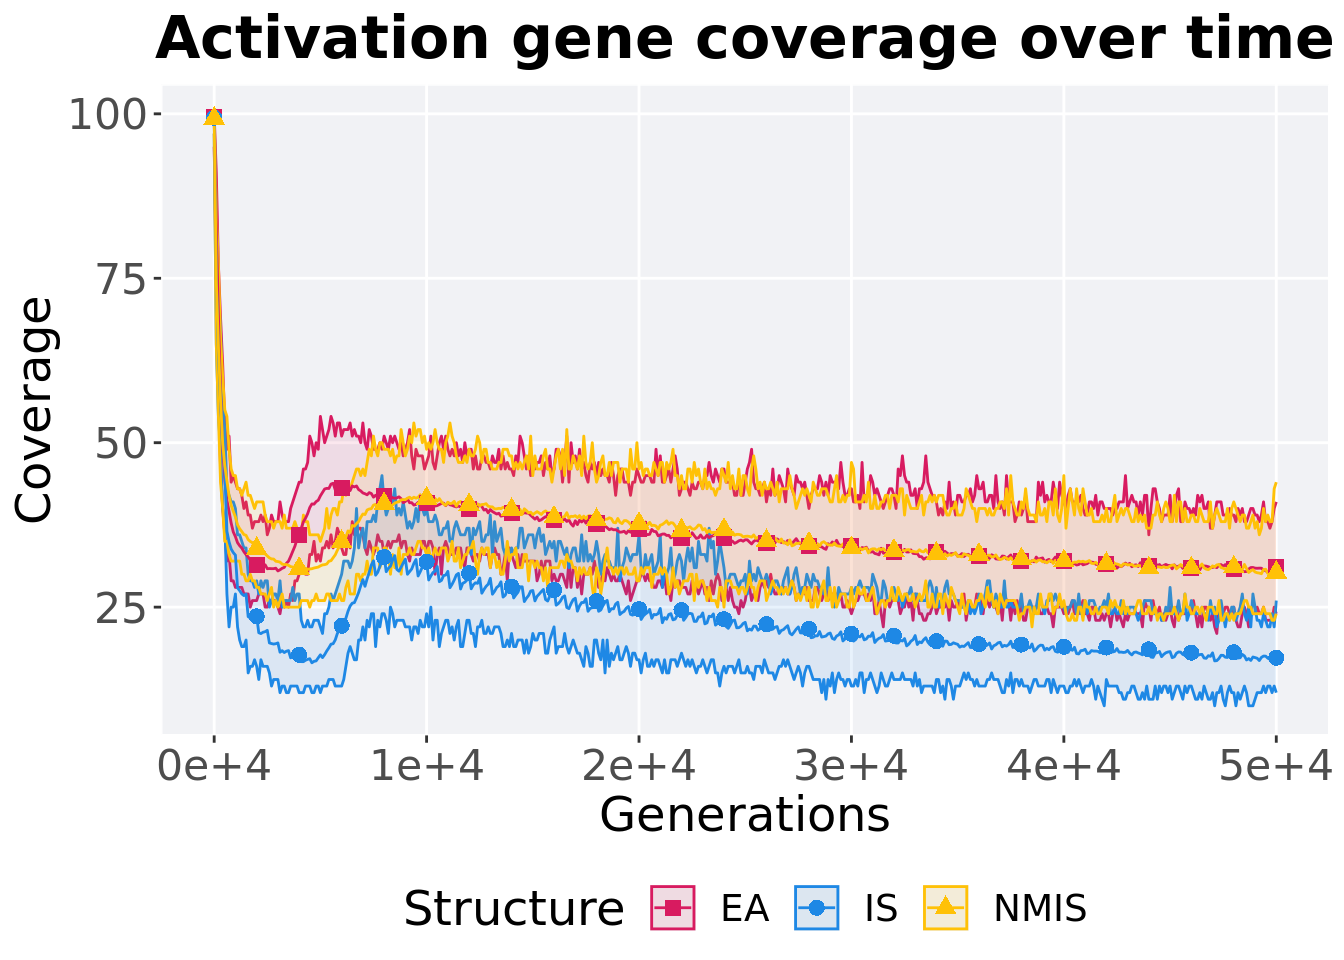
\includegraphics{demo_files/figure-latex/base-mpe-act-lex-ot-1.pdf}

\hypertarget{end-of-50000-generations-8}{%
\subsubsection{End of 50,000 generations}\label{end-of-50000-generations-8}}

Activation gene coverage in the population at the end of 50,000 generations.

\begin{Shaded}
\begin{Highlighting}[]
\CommentTok{### end of run}
\KeywordTok{filter}\NormalTok{(base_over_time, Diagnostic }\OperatorTok{==}\StringTok{ 'MULTIPATH_EXPLORATION'} \OperatorTok{&}\StringTok{ `}\DataTypeTok{Selection}\CharTok{\textbackslash{}n}\DataTypeTok{Scheme}\StringTok{`} \OperatorTok{==}\StringTok{ 'LEXICASE'} \OperatorTok{&}\StringTok{ }\NormalTok{Generations }\OperatorTok{==}\StringTok{ }\DecValTok{50000}\NormalTok{) }\OperatorTok
\StringTok{  }\KeywordTok{ggplot}\NormalTok{(., }\KeywordTok{aes}\NormalTok{(}\DataTypeTok{x =}\NormalTok{ Structure, }\DataTypeTok{y =}\NormalTok{ pop_act_cov, }\DataTypeTok{color =}\NormalTok{ Structure, }\DataTypeTok{fill =}\NormalTok{ Structure, }\DataTypeTok{shape =}\NormalTok{ Structure)) }\OperatorTok{+}
\StringTok{  }\KeywordTok{geom_flat_violin}\NormalTok{(}\DataTypeTok{position =} \KeywordTok{position_nudge}\NormalTok{(}\DataTypeTok{x =} \FloatTok{.2}\NormalTok{, }\DataTypeTok{y =} \DecValTok{0}\NormalTok{), }\DataTypeTok{scale =} \StringTok{'width'}\NormalTok{, }\DataTypeTok{alpha =} \FloatTok{0.3}\NormalTok{) }\OperatorTok{+}
\StringTok{  }\KeywordTok{geom_point}\NormalTok{(}\DataTypeTok{position =} \KeywordTok{position_jitter}\NormalTok{(}\DataTypeTok{height =} \FloatTok{.05}\NormalTok{, }\DataTypeTok{width =} \FloatTok{.05}\NormalTok{), }\DataTypeTok{size =} \FloatTok{1.5}\NormalTok{, }\DataTypeTok{alpha =} \FloatTok{0.5}\NormalTok{) }\OperatorTok{+}
\StringTok{  }\KeywordTok{geom_boxplot}\NormalTok{(}\DataTypeTok{color =} \StringTok{'black'}\NormalTok{, }\DataTypeTok{width =} \FloatTok{.2}\NormalTok{, }\DataTypeTok{outlier.shape =} \OtherTok{NA}\NormalTok{, }\DataTypeTok{alpha =} \FloatTok{0.0}\NormalTok{) }\OperatorTok{+}
\StringTok{  }\KeywordTok{scale_shape_manual}\NormalTok{(}\DataTypeTok{values=}\NormalTok{SHAPE)}\OperatorTok{+}
\StringTok{  }\KeywordTok{scale_y_continuous}\NormalTok{(}
    \DataTypeTok{name=}\StringTok{"Coverage"}
\NormalTok{  ) }\OperatorTok{+}
\StringTok{  }\KeywordTok{scale_x_discrete}\NormalTok{(}
    \DataTypeTok{name=}\StringTok{"Structure"}
\NormalTok{  ) }\OperatorTok{+}
\StringTok{  }\KeywordTok{scale_colour_manual}\NormalTok{(}\DataTypeTok{values =}\NormalTok{ cb_palette) }\OperatorTok{+}
\StringTok{  }\KeywordTok{scale_fill_manual}\NormalTok{(}\DataTypeTok{values =}\NormalTok{ cb_palette) }\OperatorTok{+}
\StringTok{  }\KeywordTok{ggtitle}\NormalTok{(}\StringTok{'Final activation gene coverage'}\NormalTok{)}\OperatorTok{+}
\StringTok{  }\NormalTok{p_theme }\OperatorTok{+}\StringTok{ }\KeywordTok{coord_flip}\NormalTok{()}
\end{Highlighting}
\end{Shaded}

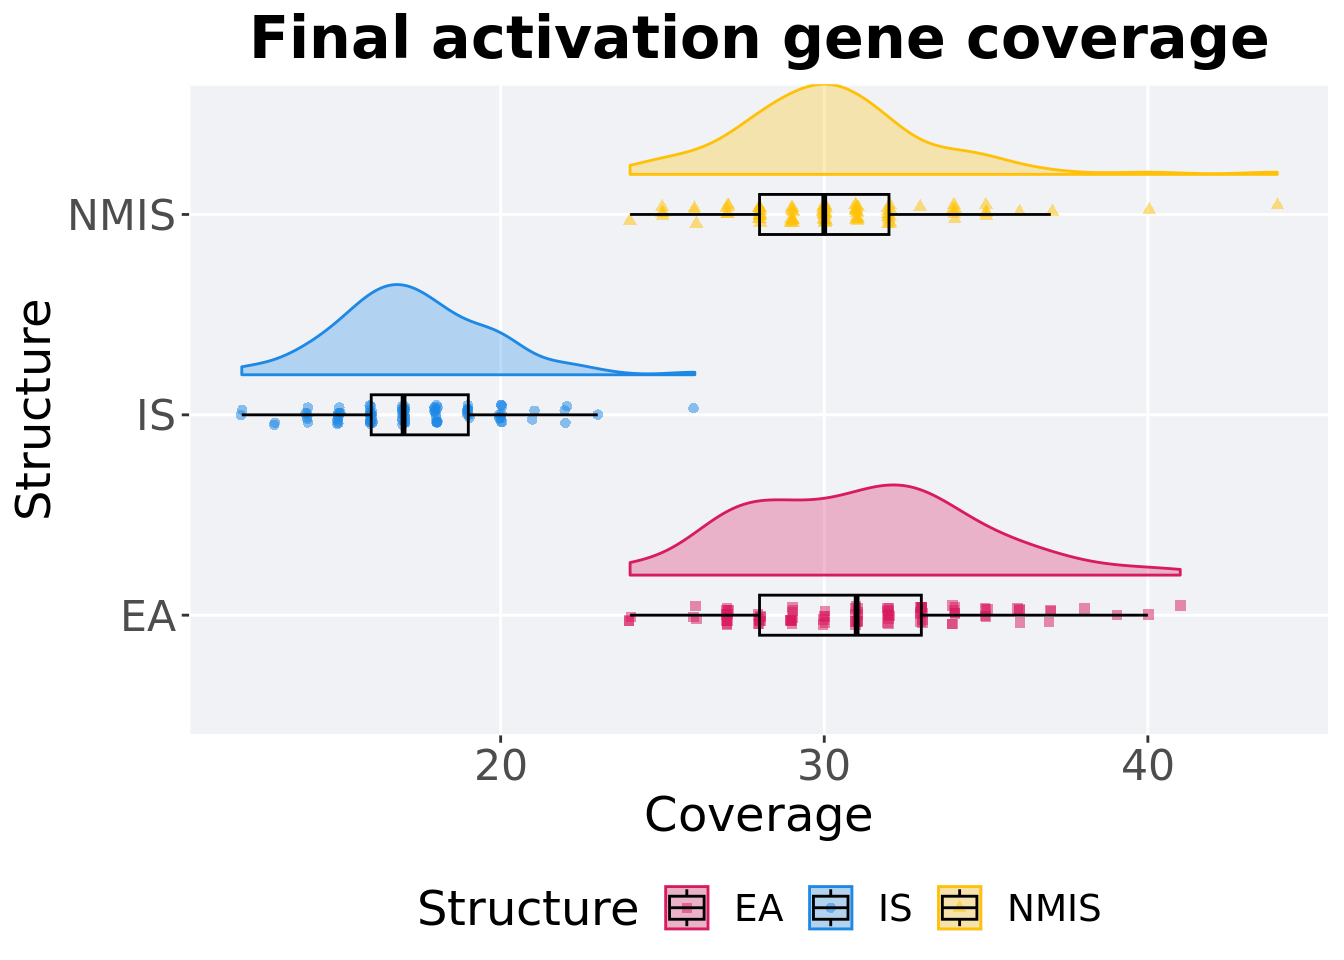
\includegraphics{demo_files/figure-latex/base-mpe-act-lex-end-1.pdf}

\hypertarget{stats-27}{%
\paragraph{Stats}\label{stats-27}}

Summary statistics for activation gene coverage.

\begin{Shaded}
\begin{Highlighting}[]
\NormalTok{coverage =}\StringTok{ }\KeywordTok{filter}\NormalTok{(base_over_time, Diagnostic }\OperatorTok{==}\StringTok{ 'MULTIPATH_EXPLORATION'} \OperatorTok{&}\StringTok{ `}\DataTypeTok{Selection}\CharTok{\textbackslash{}n}\DataTypeTok{Scheme}\StringTok{`} \OperatorTok{==}\StringTok{ 'LEXICASE'} \OperatorTok{&}\StringTok{ }\NormalTok{Generations }\OperatorTok{==}\StringTok{ }\DecValTok{50000}\NormalTok{)}
\NormalTok{coverage}\OperatorTok{$}\NormalTok{Structure =}\StringTok{ }\KeywordTok{factor}\NormalTok{(coverage}\OperatorTok{$}\NormalTok{Structure, }\DataTypeTok{levels=}\KeywordTok{c}\NormalTok{(}\StringTok{'EA'}\NormalTok{,}\StringTok{'NMIS'}\NormalTok{,}\StringTok{'IS'}\NormalTok{))}
\NormalTok{coverage }\OperatorTok
\StringTok{  }\KeywordTok{group_by}\NormalTok{(Structure) }\OperatorTok
\StringTok{  }\NormalTok{dplyr}\OperatorTok{::}\KeywordTok{summarise}\NormalTok{(}
    \DataTypeTok{count =} \KeywordTok{n}\NormalTok{(),}
    \DataTypeTok{na_cnt =} \KeywordTok{sum}\NormalTok{(}\KeywordTok{is.na}\NormalTok{(pop_act_cov)),}
    \DataTypeTok{min =} \KeywordTok{min}\NormalTok{(pop_act_cov, }\DataTypeTok{na.rm =} \OtherTok{TRUE}\NormalTok{),}
    \DataTypeTok{median =} \KeywordTok{median}\NormalTok{(pop_act_cov, }\DataTypeTok{na.rm =} \OtherTok{TRUE}\NormalTok{),}
    \DataTypeTok{mean =} \KeywordTok{mean}\NormalTok{(pop_act_cov, }\DataTypeTok{na.rm =} \OtherTok{TRUE}\NormalTok{),}
    \DataTypeTok{max =} \KeywordTok{max}\NormalTok{(pop_act_cov, }\DataTypeTok{na.rm =} \OtherTok{TRUE}\NormalTok{),}
    \DataTypeTok{IQR =} \KeywordTok{IQR}\NormalTok{(pop_act_cov, }\DataTypeTok{na.rm =} \OtherTok{TRUE}\NormalTok{)}
\NormalTok{  )}
\end{Highlighting}
\end{Shaded}

\begin{verbatim}
## # A tibble: 3 x 8
##   Structure count na_cnt   min median  mean   max   IQR
##   <fct>     <int>  <int> <int>  <dbl> <dbl> <int> <dbl>
## 1 EA          100      0    24     31  31.2    41     5
## 2 NMIS        100      0    24     30  30.3    44     4
## 3 IS          100      0    12     17  17.3    26     3
\end{verbatim}

Kruskal--Wallis test provides evidence of difference among activation gene coverage.

\begin{Shaded}
\begin{Highlighting}[]
\KeywordTok{kruskal.test}\NormalTok{(pop_act_cov }\OperatorTok{~}\StringTok{ }\NormalTok{Structure, }\DataTypeTok{data =}\NormalTok{ coverage)}
\end{Highlighting}
\end{Shaded}

\begin{verbatim}
## 
##  Kruskal-Wallis rank sum test
## 
## data:  pop_act_cov by Structure
## Kruskal-Wallis chi-squared = 201.31, df = 2, p-value < 2.2e-16
\end{verbatim}

Results for post-hoc Wilcoxon rank-sum test with a Bonferroni correction on activation gene coverage.

\begin{Shaded}
\begin{Highlighting}[]
\KeywordTok{pairwise.wilcox.test}\NormalTok{(}\DataTypeTok{x =}\NormalTok{ coverage}\OperatorTok{$}\NormalTok{pop_act_cov, }\DataTypeTok{g =}\NormalTok{ coverage}\OperatorTok{$}\NormalTok{Structure, }\DataTypeTok{p.adjust.method =} \StringTok{"bonferroni"}\NormalTok{,}
                     \DataTypeTok{paired =} \OtherTok{FALSE}\NormalTok{, }\DataTypeTok{conf.int =} \OtherTok{FALSE}\NormalTok{, }\DataTypeTok{alternative =} \StringTok{'l'}\NormalTok{)}
\end{Highlighting}
\end{Shaded}

\begin{verbatim}
## 
##  Pairwise comparisons using Wilcoxon rank sum test with continuity correction 
## 
## data:  coverage$pop_act_cov and coverage$Structure 
## 
##      EA     NMIS  
## NMIS 0.077  -     
## IS   <2e-16 <2e-16
## 
## P value adjustment method: bonferroni
\end{verbatim}

\bibliography{book.bib,packages.bib}

\end{document}
